% \usepackage{siunitx}
\setlength\parskip{\smallskipamount}

% LS, runs, phases, Tier, to ease conventions
\newcommand{\ns}{\ensuremath{\,\text{ns}}\xspace}
\newcommand{\COTwo}{$\text{CO}_2$\xspace}
\newcommand{\LSTwo}{LS~$2$\xspace}
\newcommand{\LSThree}{LS~$3$\xspace}
\newcommand{\LSFour}{LS~$4$\xspace}
\newcommand{\LSFive}{LS~$5$\xspace}
\newcommand{\RunOne}{Run~$1$\xspace}
\newcommand{\RunTwo}{Run~$2$\xspace}
\newcommand{\RunThree}{Run~$3$\xspace}
\newcommand{\RunFour}{Run~$4$\xspace}
\newcommand{\RunFive}{Run~$5$\xspace}
\newcommand{\RunSix}{Run~$6$\xspace}
\newcommand{\PhaseOne}{Phase~$1$\xspace}
\newcommand{\PhaseTwo}{Phase~$2$\xspace}
\newcommand{\TierZero}{Tier-$0$\xspace}
\newcommand{\TierOne}{Tier-$1$\xspace}
\newcommand{\TierTwo}{Tier-$2$\xspace}
\newcommand{\TierThree}{Tier-$3$\xspace}

\newcommand{\ROOT}{\textsc{ROOT}}

%Odd page for section;
\let\oldsection\section   % save original
\renewcommand{\section}{%
  \cleardoublepage
  \oldsection
}

% from https://design-guidelines.web.cern.ch/guidelines/ppt-colours
\definecolor{myblue}{RGB}{0,51,160} % Pantone 286C
\definecolor{myorange}{RGB}{225,94,50}
\definecolor{mycyan}{RGB}{97,197,211}
\colorlet{tableheader}{myblue!60}
\colorlet{tablerowheader}{myblue!20}
\newcommand{\trh}{\cellcolor{tablerowheader}}
\colorlet{tablerowhighlight}{myblue!5}
\newcommand{\trl}{\cellcolor{tablerowhighlight}}

%\hypersetup{%
%pdfauthor={D. Elvira, F. Ferri, et al.},%
%pdftitle={CMS Offline Software and Computing for HL-LHC CDR},%
%pdfsubject={CMS},%
%pdfkeywords={CMS, computing}
%}

%Phat: Put the cover file separately, so it will print on a full-color page, and not part of the page counting
%\thispagestyle{empty}
%\includepdf{figs/CoverIllustration-CDR.pdf}
%\cleardoublepage


\includegraphics[width=0.15\textwidth]{figs/CMSlogo_outline_black_nolabel_May2014}

\vspace*{-25mm}

{\large\sffamily
\hspace*{\fill}\parbox{55mm}
{\sffamily\bfseries {CERN-LHCC-2026-003} \\[2mm]
{\sffamily\bfseries {LHCC-G-186}}         \\[2mm]
{\sffamily\bfseries {March 24, 2026}}     \\[2mm] 
}}

\vspace{2cm}

\begin{center}
{\Large\sffamily\bfseries CMS Offline Software and Computing for HL-LHC}\\[5mm]
{\Large\sffamily\bfseries Conceptual Design Report}\\[10mm]
{\Large\sffamily CMS Collaboration}
\end{center}

\vspace{1cm}

\begin{center}
\textbf{\Large Abstract}
\end{center}

This Conceptual Design Report outlines a plan for an Offline Software \& Computing system to enable the physics program of the CMS experiment during the High-Luminosity LHC era, due to start in 2030. Challenges are driven by the increase in detector complexity and data volumes, while emerging computing technologies offer opportunities, though at a high cost of adaptation. Projections of CMS’s computing resource needs for the 2030--2039 period are provided, as well as a high-level technical roadmap for the 2026--2030 preparation period. 

\vspace*{\fill}

\cleardoublepage


%\title{CMS Offline Software and Computing for HL-LHC\\[.5cm] Conceptual Design Report}
%\author{}
%\abstract{
%This Conceptual Design Report outlines a plan for an Offline Software \& Computing system to enable the physics program of the CMS experiment during the High-Luminosity LHC era, due to start in 2030. Challenges are driven by the increase in detector complexity and data volumes, while emerging computing technologies offer opportunities, though at a high cost of adaptation. 
%Projections of CMS’s computing resource needs for the 2030--2039 period are provided, as well as a high-level technical roadmap for the 2026--2030 preparation period. 
%}
%\date{\today}

%%%%%%%%%%%%%%%%%%%%%%%%%%%%%%%%%%%%%%%%%%%%%%%%%%%%%%%%%%%%%%%%%%%%%%%%%%%%%%%%
% \begin{document}\cmsNoteHeader{TDR-24-001}

%\maketitle
\pagestyle{fancy}

%%%%%%%%%%%%%%%%%%%%%%%%%%%%%%%%%%%%%%%%%%%%%%%%%%%%%%%%%%%%%%%%%%%%%%%%%%%%%%%%
%
% List of editors: Comment out later please
%
%%%%%%%%%%%%%%%%%%%%%%%%%%%%%%%%%%%%%%%%%%%%%%%%%%%%%%%%%%%%%%%%%%%%%%%%%%%%%%%%

%\textbf{List of Initial Editors}
%\begin{itemize}
%    \item Main Editors: D. Elvira, F. Ferri, L. Sexton-Kennedy, P. Srimanobhas, J. Letts, Nick Smith
%    \item Special readers (ARC members): M. Klute, L. Bauerdick, D. Piparo, O. Gutsche, G. Hamel de Monchenault
%\end{itemize}

%\begin{enumerate}
%      \item Executive Summary: D. Elvira
%      \item Introduction: J. Letts, K. Ellis, D. Elvira; J. Martins, S. Rappoccio (physics - now a section
%    \item Management Framework: L. Sexton-Kennedy, J. Letts, K. Ellis, D. Elvira
%    \item computing model (combination of old Section 4, 5, and 7): T. Boccali, O. Gutsche, B. Jayatilaka, C. Wissing, J. Letts, D. Elvira
%    \item Core Software: M. Kortelainen, L. Sexton-Kennedy
%    \item Event Generation: S. Bhattacharya, B. Bilin, M. Lu
%    \item Detector Simulation: S. Bein, V. Ivantchenko, K. Pedro
%    \item Data Reconstruction: J. Fernández, M. Nguyen
%    \item workflow management: D. Ciangottini, A. Perez-Calero Yzquierdo, L. Sexton-Kennedy
%    \item End-User Analysis: L. Gray, P. Lenzi, L. Sexton-Kennedy
    %\item Workflow management: A. Perez Calero, D. Ciangottini, L. Sexton-Kennedy % Duplicate
%    \item Evolution of the Computing Infrastructure (combination of old Section 5, 7, 8, and 11): T. Boccali, O. Gutsche, B. Jayatilaka, C. Wissing, A. Melo, M. Giffels, D. Hufnagel, D. Spiga, J. Letts, N. Smith
%    \item Testing and Validation (new chapter): J-R. Vlimant, H. Brandao Malbouisson, D. Kovalskyi, P. Srimanobhas, F. Ferri, A. Di Florio
%    \item Computing resource estimates and projections: J. Flix, D. Lange, D. Elvira, F. Ferri, J. Letts; Hardware Evolution Trends (now a subsection): D. Hufnagel, D. Spiga
%    \item technical roadmapmap (new chapter for the detailed tables, timelines):  P. Srimanobhas, D. Elvira
%    \item Summary: D. Elvira
    
%\end{enumerate}

\clearpage

%\textbf{Editorial notes, 2024-11-11}
%\begin{itemize}
%    \item This version of the document is the first iteration after receiving the early readers comments:
%    \begin{itemize}
%        \item a major refactoring has been made to make the structure clearer;
%        \item a significant number of early readers comments have been implemented;
%        \item those that have not yet been implemented are in progress.
%    \end{itemize}
%    \item A first set of results for the baseline scenario has been presented at the O\&C week \href{https://indico.cern.ch/event/1460070/#33-resource-estimations-and-pr} and is included in this document; the text of the corresponding sections is being edited;
%    \begin{itemize}
%        \item the variation on the baseline scenario are being computed
%        \item the final resource projections including the effect of the R\&D activities, and an estimate of the 
%    \end{itemize}
%    \item Chapter 10 ``End-user analysis'' is under revision
%    \item Chapter 11 ``Evolution of the computing infrastructure'' is being worked on
%    \item As there will be no document from PPD detailing the plans for \PhaseTwo, a chapter/section on the PPD subjects is being included in this document, with emphasis on the alignment and calibration (and related infrastructure and services) and testing and validation of offline software and physics simulation.
%\end{itemize}

%\textbf{Editorial notes, September 2024}

%\begin{itemize}

%\item This document was a refactoring of the draft CDR document as it was on May 20, 2024. 
%Subsequent changes to that document have not been included, of which there are changes to the Generator and possibly Reconstruction chapters.

%\item Each major offline software and computing area (core software, generators, simulation, reconstruction, workflow management, and end-user analysis) has been given its own chapter and the style made more similar, with a summary table of major R\&D lines given at the end, with any impact especially on computing resources or \gls{GPU} offload. 

%\item The chapters on the computing model and its simulation have been edited extensively, with a new Chapter~\ref{sec:Model} describing the high-level computing model while simulations of the computing model based on particular LHC and CMS-specific scenarios and their variations is moved to Chapter~\ref{sec:EvilPlots}.

%\item Chapter~\ref{sec:Infrastructure} is still undergoing editing. The idea behind the chapter is that the various offline software R\&D activities (especially offload to \glspl{GPU}), analysis requirements, and data transfer and I/O bandwidth to storage requirements (yet to be written down in Chapter~\ref{sec:Bandwidth}) will place boundary conditions on what is possible and what will not scale. However, the reordering of the text from various chapters of the original document can give one a sense of how this chapter could flow.

%\item Two new chapters are proposed, one Chapter~\ref{sec:Validation} on Testing and Validation and another Chapter~\ref{sec:Roadmap} on the technical roadmap. 

%\end{itemize}

%\textbf{Editorial notes, April 2025}

%\begin{itemize}

%\item \textbf{Executive summary} added.

%\item \textbf{Introduction} chapter significantly updated to include a short summary of how the physics program triggers computing needs, previously discussed in a physics overview chapter (removed).

%\item \textbf{Management framework} chapter updated to explain the role of the new Project Office and \gls{CB} subgroup

%\item \textbf{Offline software} chapters significantly updated: computing performance measurements, R\&D tables.

%\item \textbf{Computing model}. Completed content, added/updated parameter values.

%\item \textbf{Computing Infrastructure} chapter completely re-written, R\&D activities introduced and described. 

%\item \textbf{Computing resources and projections} chapter has been written from scratch. it contains a description of the compound R\&D scenarios, the mathematical expression used in the simulation of the computing model to predict resource needs, and the plots with the \gls{CPU}, disk, tape resource needs during the \PhaseTwo period for the baseline and several R\&D scenarios. 

%\item \textbf{Validation and Testing} chapter is mostly complete, contributed by PPD in collaboration with O\&C computing operations. Sections on software performance and computing infrastructure scalability for testing and validation are still missing, and some additions and corrections are pending throughout the chapter.

%\item \textbf{Technical roadmap} chapter written from scratch, contains a table with a high-level description of a schedule with deliverables and milestones, including the \gls{CSA} challenge.

%\item \textbf{Summary} chapter has been added with a short paragraph that needs to evolve as we digest the resource projections further.

%\end{itemize}

%\textbf{Editorial notes, November 6, 2025}

%\begin{itemize}

%\item \textbf{ARC questions and comments} on CDR v2 were addressed. Answers are available through CADI.

%\item \textbf{Executive summary} was significantly modified following ARC comments. Missing chapters were added.

%\item \textbf{Computing model}. LHC and CMS running conditions were updated. Storage policy was significantly revised.

%\item \textbf{Computing resources and projections}. Compound R\&D scenarios were updated and so were resource needs projections. The WLCG prediction for price/performance-capacity evolution was updated.

%\item \textbf{Validation and Testing}. Missing sections were added.

%\item \textbf{Summary}. The placeholder text was replaced by statements consistent with the outcome of the result projections exercise.

%\end{itemize}

%\textbf{Editorial notes, November 27, 2025}

%\begin{itemize}

%\item \textbf{Language tools} were used to enforce compliance with CMS publication committee rules (CMS-LLM) and grammar rules (Grammarly).

%\end{itemize}

%\textbf{List of FIXMEs}

%Here is list of FIXMEs that still need to be implemented.

%\FIXME{GENERAL: Some R\&D lines are out of order in the text relative to the summary tables in each section. This will be fixed at the end of the review process.}

%\FIXME{GENERAL: A small section on data preservation will be added to the post April 2025 version. ESK:I've condensed the DPOA group's document to a page and a 1/2.}

%\FIXME{EXECSUM, Testing and validation: to be added when the corresponding chapter is implemented by PPD in collaboration with O\&C Computing Operations.}

%\FIXME{WORKFLOW MGMT: Need to answer overleaf comments and improve the connection between the WorkMgmt.x activities and the many efforts mentioned as ''desired'' or that ''should be undertaken'' in the text which do not seem to have an ''activity home'' or even be part of the plan.}

%\FIXME{WORKFLOW MGMT: What are the unified tools employed by P\&R? What's P\&R?}

%\FIXME{ANALYSIS: All the tools mentioned must be referenced.}

%\FIXME{ANALYSIS: Are Jupyter and iPython referenced before?}


%\FIXME{ANALYSIS:Missing text in ''During, and''} 

%\FIXME{ANALYSIS: CITATIONS NEEDED FOR DASK AND COLUMNFLOW.} 

%\FIXME{ANALYSIS: I don't understand what you mean by share columns of an output that are available to anyone anyway.}

%\FIXME{ANALYSIS: CITATIONS NEEDED FOR SERVICE-X, SKYHOOK, AND TILED.} 

%\FIXME{ANALYSIS: ADD MOTIVATION FOR THIS POINT.}

%\FIXME{ANALYSIS: What's a likelihood distribution? Do you mean likelihood approximations / simplified likelihoods?}

%\FIXME{ANALYSIS: CITATIONS NEEDED FOR PARSL, WORKQUEUE, SPARK.}

%\FIXME{ANALYSIS: Why do you pick 1-d to develop in a subsection and not other requirements?}

%\FIXME{ANALYSIS: CITATION NEEDED FOR CITATION FOR PARTICLENET.}

%\FIXME{ANALYSIS: CITATION FOR for pyhf and z-fit.}

%\FIXME{ANALYSIS: The description of the visualization plan is very good but the level of detail is probably too much as compared with other tools elsewhere in the document. Should we reduce it to concepts, feature justification, risk analysis, etc. for the CDR? Should there be a visualization activity in the summary R\&D table for analysis?}

%\FIXME{ANALYSIS: Add reference to Fireworks.}

%\FIXME{ANALYSIS: Check if \gls{AAA} is referenced before this mention.}

%\FIXME{ANALYSIS: Add reference to REve.}

%\FIXME{ANALYSIS: It is not clear what is the organization in CMS that plans and leads this work. Is it the Common Analysis Tools group, which does not live in O\&C? We say many times that CMS should collaborate or work with this or the other group but we do not say who ''we'' (the people writing this plan) are. This needs to be clear. If it is the \gls{CAT}, do they know that they have to execute the plan described here? Were they active participants in writing the content of this Chapter? Have they endorsed it?}

%\FIXME{ANALYSIS: Daniel quantified impact of activities in tables. Pleases verify.}

% \FIXME{COMP INFRAS: What does ''weakly defined'' mean in this case}

% \FIXME{COMP INFRAS: Add reference to \gls{ESCAPE}.}

% \FIXME{COMP INFRAS: Do you mean table 1? Please add the reference}

% \FIXME{COMP INFRAS: We may consider adding the activities to the table (if critical) and explicitly mention in the text that they are external. Then, we can add a paragraph on the impact of computing infrastructure R\&D in Chapter 13 and mention external risks and dependencies.}

% \FIXME{COMP INFRAS: Add black horizontal lines separating activities, in description, skip it in impact if it is a common impact.}

%\FIXME{(RECONSTRUCTION: the number of CMS channels requiring some form of correction, be it calibration or synchronization, will be of the order of 30 millions - TBC)}

%\FIXME{TESTING AND VALIDATION: Corrections and additions are pending and indicated with red text. Sections on software performance and computing infrastructure scalability for testing and validation are still missing.}

%\FIXME{RESOURCES: Pie charts with the post-R\&D time shares will be added to the post-April version.}

% \FIXME{RESOURCES: Here we should discuss, at least, qualitatively how the R\&D described in the computing infrastructure chapter improves it. We should also discuss how R\&D in other areas (software, data formats) would affect the use of computing infrastructure. (One example is the impact of data formats on networking needs.) In cases for which it is possible to make quantitative assessments, we may think of the possibility to add this information as an input to the estimation of computing resources. We would even think about the possibility to add more resource types to the estimations (beyond tape, disk, \gls{CPU}), such as networking.}

%\FIXME{RESOURCES: Need to add mention to R\&D for event mixing}

%\FIXME{CONCLUSIONS AND OUTLOOK: Awaiting finalization of results and interpretation.}

\clearpage

\section*{Editors}

D.~Elvira, F.~Ferri, J.~Letts, E.~Sexton-Kennedy.

\oldsection*{Chapter editors}

S.~Bhattacharya, S.~Bein, B.~Bilin, T.~Boccali, T.~Bose, H.~Brandao Malbouisson, D.~Ciangottini, A.~Di Florio, K.~Ellis, J.~Fernández,  J.~Flix, M.~Giffels, L.~Gray, O.~Gutsche, D.~Hufnagel, V.~Ivantchenko, B.~Jayatilaka, C.~Koraka, M.~Kortelainen,  D.~Kovalskyi, D.~Lange, P.~Lenzi, M.~Lu, J.~Martins, A.~Melo, M.~Nguyen, K.~Pedro, A.~Pérez-Calero Yzquierdo, D.~Piparo, S.~Rappoccio, N.~Smith, D.~Spiga, P.~Srimanobhas, J-R.~Vlimant, C.~Wissing.  

\oldsection*{Cover Page}

S.~Cittolin.

\oldsection*{Acknowledgements}

This document is the result of years of work by many colleagues within the CMS offline software and computing organization, and across most CMS coordination areas. Consultation with software development teams and computing organizations external to CMS were also priceless. We want to thank everyone involved for their contributions, which included discussions and decision-making sessions, as well as the text and numerical estimates presented in this report. In particular, we would like to thank James Letts and Danilo Piparo, who started the conceptual design process and recruited the initial team of editors while serving as coordinators of the offline and computing area. Our appreciation is also extended to Lothar Bauerdick, Oliver Gutsche, Gautier Hamel de Monchenault, Markus Klute, and Danilo Piparo, who served as internal readers of evolving drafts, offering their invaluable experience and wisdom through the process.

\clearpage
\tableofcontents

%%%%%%%%%%%%%%%%%%%%%%%%%%%%%%%%%%%%%%%%%%%%%%%%%%%%%%%%%%%%%%%%%%%%%%%%%%%%%%%%
%
% EXECUTIVE SUMMARY AND OVERVIEW
%
%%%%%%%%%%%%%%%%%%%%%%%%%%%%%%%%%%%%%%%%%%%%%%%%%%%%%%%%%%%%%%%%%%%%%%%%%%%%%%%%
% \clearpage
% \input{tex/00_executive_summary.tex}
\section*{Executive summary}
\addcontentsline{toc}{section}{Executive summary}
\label{sec:execsum}

The High-Luminosity LHC (HL-LHC) will define the forefront of particle physics in the 2030s, enabling the CMS experiment to pursue a uniquely rich and ambitious physics program. With an integrated luminosity of up to 3000 fb$^{-1}$ and instantaneous luminosities reaching 5–7.5 $\times10^{34} $cm$^{-2}$s$^{-1}$, CMS will perform precision studies of the Higgs sector, including measurements of the Higgs boson self-coupling and total width, extend sensitivity to rare standard model processes, and significantly broaden its discovery reach for physics beyond the standard model. Searches for dark matter, long-lived particles, and other exotic signatures will particularly benefit from the large data sets and enhanced trigger capabilities. Realizing this physics potential critically depends on the ability of the CMS software and computing system to record, process, simulate, and analyze data of unprecedented volume and complexity in a timely and sustainable manner.

The HL-LHC operating conditions and the CMS detector upgrades pose exceptional challenges for offline software and computing. Average pileup levels of 150--200 simultaneous proton–proton interactions per bunch crossing\footnote{Pileup running conditions were updated in July 2025 from 140--200 to 150--200 upon a recommendation from the LHC Program Coordination Group, and an agreement with WLCG and the other LHC experiments} lead to substantially larger event sizes and sharply increased CPU requirements for simulation and reconstruction. In addition to pileup, the upgraded detector introduces a significant rise in intrinsic event complexity, with an order-of-magnitude increase in readout channels driven primarily by the new tracker and high-granularity calorimeter, together with the inclusion of precision timing information. These effects act in combination to increase processing time, data volumes, and pressure on storage and network infrastructure well beyond those experienced in previous LHC runs.

In parallel, the HL-LHC era offers new opportunities at the level of data acquisition and triggering that are explored to maximize the CMS physics reach. The upgraded Level-1 and high-level trigger systems enable higher accept rates and more sophisticated selections, including extensive use of data scouting. Scouting at both trigger levels allows CMS to record very high-rate samples with reduced event content, opening sensitivity to signatures that would otherwise be inaccessible within conventional trigger bandwidths. While these approaches significantly enhance physics potential, they introduce additional challenges for downstream computing and, in particular, for storage, as scouting data sets may constitute a substantial fraction of the total recorded data volume.

The CMS \gls{OANDC} strategy is developed assuming a flat or near-flat funding profile over the HL-LHC period. In earlier LHC phases, this assumption was viable due to sustained gains in computing price-to-performance, which absorbed much of the growth in resource requirements. Recent trends, however, show a clear slowdown in these improvements, especially for disk storage. When combined with order-of-magnitude increases in data volumes and multi-fold increases in processing time, this evolution makes it increasingly difficult to deliver the HL-LHC computing program within constant resources. This tension is most pronounced for storage, where projected disk and tape needs exceed expected available capacity even under optimistic assumptions.

Meeting these challenges requires a comprehensive and sustained research and development program. While some components of the current CMS software and computing infrastructure scale adequately, others do not and must be significantly redesigned. R\&D is therefore essential to reduce CPU time per event, control event and data format sizes, and enable efficient use of heterogeneous computing resources, including GPUs and high-performance computing facilities. Key elements include algorithmic and software optimizations, fast and machine-learning-based simulation techniques, performance-portable frameworks, and new models for workflow, data management, and analysis that can operate effectively in a heterogeneous and increasingly centralized computing landscape.

This \gls{CDR} describes the CMS HL-LHC offline software and computing system and the associated R\&D program in detail. It defines a baseline computing model and a set of alternative scenarios incorporating the anticipated impact of R\&D activities, together with assessments of technical risk and likelihood of adoption. Quantitative projections of CPU, disk, and tape resource needs over the HL-LHC lifetime are presented, and the extent to which R\&D can mitigate the gap between required and available resources is evaluated. A high-level technical roadmap outlines milestones and decision points guiding the evolution of the system toward readiness for HL-LHC data-taking.

The conclusion of this study is that sustained and successful R\&D is indispensable for enabling the full CMS HL-LHC physics program under realistic budget constraints. While advances in software performance, heterogeneous computing, and fast simulation can substantially alleviate the pressure for processing, storage (both disk and tape) remains the most critical and least tractable challenge. Even assuming broad success of the planned R\&D program, projected disk and tape needs are expected to exceed available resources. Addressing this gap will require continued innovation in data reduction, storage technologies, and data management strategies, as well as coordinated action across the CMS Collaboration and the wider LHC computing community.

The \gls{CDR} process in CMS involved many people and groups over the years. Some elements were completed earlier, while others were finalized or updated at the end of 2025. Recent developments in computing technologies, computational, and
experimental techniques are bringing opportunities that are not fully
explored by CMS yet. Most notably, major breakthroughs in \gls{AI} made during the CDR process, demand continuous updates to the CMS \gls{AI} strategy, which are not fully represented in this document. 
 
%%%%%%%%%%%%%%%%%%%%%%%%%%%%%%%%%%%%%%%%%%%%%%%%%%%%%%%%%%%%%%%%%%%%%%%%%%%%%%%%
%
% INTRODUCTION
%
%%%%%%%%%%%%%%%%%%%%%%%%%%%%%%%%%%%%%%%%%%%%%%%%%%%%%%%%%%%%%%%%%%%%%%%%%%%%%%%%
% \clearpage
% \input{tex/01_introduction.tex}
\glsresetall
\clearpage
\section{Introduction}
\label{sec:Introduction}

This document presents a conceptual design for the \gls{OANDC} system of the upgraded CMS detector, intended to start operating at CERN's LHC in 2030.

The LHC upgrade during the third long shutdown (\LSThree), currently scheduled to begin in July 2026 and last until the end of 2029, will enable the collider to deliver much higher luminosity to the experiments. The current baseline planning assumes that the \gls{HL-LHC} will provide instantaneous luminosities between $5\times10^{34}\mathrm{cm}^{-2}\mathrm{s}^{-1}$ and $7.5\times10^{34}\mathrm{cm}^{-2}\mathrm{s}^{-1}$, compared to about $2\times10^{34}\mathrm{cm}^{-2}\mathrm{s}^{-1}$ during \RunThree. This luminosity range corresponds to an average number of interactions per beam crossing, or ``pileup'', in the 150--200 range.

Throughout the document \RunOne refers to the first LHC period of data taking, when the LHC was operated at a proton-proton center-of-mass energy of $\sqrt{s}$ = 7~TeV (2010--2011) and 8~TeV (2012). \RunTwo and \RunThree correspond to the 2015--2018 and 2023--2026 periods at  $\sqrt{s}$ = 13~TeV and 13.6~TeV respectively, while \RunFour and \RunFive define the \gls{HL-LHC} era in 2030--2033 at $\sqrt{s}$ = 13.6~TeV and in 2036--2041 at $\sqrt{s}$ = 14~TeV. 
The LHC running conditions are the key factor in determining the values of input parameters to the CMS computing model. Conservatively, CMS considers a baseline scenario with 150 pileup interactions in \RunFour and 200 in \RunFive. Variations within this range are used to assess sensitivity and evaluate risk, which will be discussed in succeeding chapters.

% http://lhc-commissioning.web.cern.ch/schedule/LHC-long-term.htm

During \LSThree, the CMS detector, including its \gls{OANDC} component, will undergo many upgrades from its current configuration~\cite{CMS:2023gfb} to take advantage of the increased data volume.
The term \PhaseTwo CMS detector or experiment defines the upgraded version to take data in the \gls{HL-LHC} era. \PhaseOne refers to the 2017 upgrade, which consisted of a new pixel detector, as well as improvements to the \gls{HCAL} backend electronics and \gls{L1T}. Major components of the \PhaseTwo experiment include upgraded tracker~\cite{CMS:2017TrackTDR,Ceccarelli:2024mev}, muon~\cite{CMS:2017MuonTDR}, and luminosity~\cite{CMS:2021BRTDR} detectors, a high-granularity electromagnetic endcap calorimeter~\cite{CMS:2017HGCalTDR} (\gls{HGCAL}), a timing (\gls{MIP}) detector~\cite{CMS:2019MIPTDR}, as well as improvements to the \gls{DAQ}~\cite{CMS:2021DAQTDR} and the \gls{L1T} systems~\cite{CMS:2020L1TTDR}.

The planned LHC machine and detector upgrades for \PhaseTwo demand significant enhancements to the CMS \gls{OANDC} system. The larger number of detector readout channels contribute mainly by the \gls{HGCAL}, along with the higher instantaneous luminosity and trigger rates, will expand the discovery potential of the CMS experiment. They will also increase the data volume by about one order of magnitude, which will bring challenges to the scalability of the software, computer processing, storage, and network utilization. 

The goal of this \gls{CDR} is to design and describe, at the conceptual level, a computing model that fulfills the demands of the HL-LHC physics program in the context of the collider and CMS detector scenarios. The \gls{CDR} process involved many people and groups within CMS over the years. Some chapters were completed earlier, e.g., detector simulation in the fall of 2024, while others were finalized or updated at the end of 2025, such us the resource projections.
Recent progress in software and computing technologies will impact system operations and data processing in ways that are not fully evaluated yet. For instance, the acceleration in the rate of advance within the field of \gls{AI}, \gls{ML}, and heterogeneous computing during the CDR process promises transformational change in productivity and physics potential, which CMS must harvest with effort-intensive investments in infrastructure and software adaptation. 
Additionally, techniques such as Level-1 trigger scouting and other forms of real-time data reduction enable the recording of high-rate, reduced event information, that would otherwise be inaccessible within the traditional trigger and storage model. Although these topics are not fully
integrated to the baseline described in this document, they represent active areas of research and development and will influence future iterations of the CMS computing architecture and model design for the \gls{HL-LHC} era.

%Resources must be utilized efficiently by means of highly-performant software applications and minimal operational effort, as well as by completing computing requests in short and predictable time periods. Flexibility to adapt to this evolving technology landscape is the core design attribute of the computing model CMS is developing for \PhaseTwo. The computing model must enable the use of heterogeneous and high-performance computing hardware, disk, and tape storage, and networks in a flexible manner, while maintaining a unified code base that fulfills the goals mentioned above. Heterogeneous computing refers to a paradigm shift signaling a departure from traditional \gls{CPU} systems and the usage of computer systems that mix a diverse set of architectures based on a main processor and other co-processors such as \glspl{GPU}, \glspl{TPU}, and \glspl{FPGA}. The computing model must also enable the use of artificial intelligence techniques, which are permeating every component of the experiment, and benefit from dedicated software and computing infrastructure.

%This hybrid system performs tasks more efficiently in the context of a world where further growth of transistor density in traditional \gls{CPU}-based architectures brings an increase in power consumption and heat generation due to the breakdown of Dennard scaling. Heterogeneity comes, however, with added complexity, as different co-processor flavors and vendors require the use of specialized software. The development of ``performance portability'' software layers to handle hybrid systems seamlessly is one of the main challenges faced by the \gls{HL-LHC} computing program.   

\subsection{A computationally intensive physics program}

The \gls{HL-LHC} provides the opportunity to seek answers to outstanding questions in particle physics. This includes a detailed investigation of the Higgs boson sector of the \gls{SM}, precision measurements of \gls{SM} properties, and searches for rare processes including \cPqb\ quark physics signatures, searches for physics \gls{BSM}, such as dark matter, and investigations into states of matter present in the primordial universe, such as the quark-gluon plasma.  
Examples of flagship analyses that will be pursued at the \gls{HL-LHC} include the measurement of the Higgs boson self-coupling, the total width of the Higgs boson  (sensitive to its decays or invisible particles), and \gls{BSM} searches for long-lived and heavy particles. 

The detector and its readout electronics will undergo substantial refurbishment during \LSThree to improve physics performance and withstand the radiation environment of the high-luminosity, enabling higher trigger rates.
%The upgraded CMS detector will have an improved tracking system, a paradigm-changing forward calorimeter, a novel detector to measure the arrival time of minimum-ionizing particles, and a groundbreaking trigger system. 
Dominated by the tracking detector, the total number of channels to be read out will increase by about a factor of~15 compared to the \PhaseOne detector.
The upgraded computing system must be able to collect, process, analyze, and simulate the resulting data sets to deliver physics results in a timely manner.
In \RunThree, CMS budgeted resources to reconstruct at least 30\% of the data promptly. The availability of additional compute resources, however, enabled CMS to reconstruct the full \gls{RAW} data set promptly. The baseline plan for \PhaseTwo aims to maintain prompt reconstruction at 100\%. Anything less would jeopardize the ability to quickly identify and address potential problems in the data, as well as the fast delivery of physics-analysis-quality data sets for discovery.

The strict demands of the physics program on the computing system will therefore require innovative strategies and a continuous effort in the years to come. The system design must also adhere to the sustainability principles of a minimal footprint and operational costs. Computing resources must be utilized efficiently through highly performant software applications and minimal operational effort, and computing requests must be completed in short, predictable time periods. Flexibility to adapt to this evolving technology landscape is the core design attribute of the computing model CMS has designed for \PhaseTwo. The computing model must enable the use of heterogeneous and high-performance computing hardware, disk and tape storage, and networks in a flexible manner, while maintaining a unified code base that fulfills the goals mentioned above. Heterogeneous computing refers to a paradigm shift signaling a departure from traditional \gls{CPU} systems and the usage of computer systems that mix a diverse set of architectures based on a main processor and other co-processors such as \glspl{GPU}, \glspl{TPU}, and \glspl{FPGA}. The computing model must also facilitate the use of techniques based on \gls{ML} and \gls{AI} in general, which are permeating every corner of the experiment. While promising a revolution in how CMS performs both operational and data-processing tasks, these techniques pose a challenge for software and computing infrastructure planning.

\subsection{A conceptual design of the CMS O\&C upgrade for HL-LHC}

This \gls{CDR} for CMS \PhaseTwo \gls{OANDC} builds on prior experience. Planning for the \PhaseTwo upgrade of O\&C began many years ago with projections of computing resource requirements based on the \RunTwo computing model. Early estimates from 2017~\cite{Sexton-Kennedy:2018bbg} and 2018~\cite{CMSCompResults} projected the resource needs to be several times greater than the expected CMS \PhaseTwo computing budget, assuming a flat profile. Building on an internal CMS report from the CMS task force on the evolution of the computing model (ECoM2X)~\cite{ecom2x}, these estimates were updated in the documents presented during the \gls{LHCC} computing model reviews in May 2020~\cite{Software:2751565} and November 2021~\cite{Software:2815292}. Given ongoing global budget uncertainties, the continued reliance on a flat budget model may no longer be a viable long-term strategy, thus introducing substantial risk. This underscores the critical role of strategic R\&D investments in mitigating emerging risks and serves as a foundational element of our planning process, providing a clear rationale for the advancements detailed later in this document.

The scope of this document is defined by the goal to provide enough detail to show that the proposed computing model satisfies, with high probability, the demands of the physics program under the expected collider and detector running scenarios. This includes a description of the elements of the computing model and how they are integrated in a coherent and sustainable system, a baseline scenario defined by a set of parameters and their values, a simulation of the computing model to estimate the baseline resource needs, as well as a comprehensive list of R\&D tasks to bridge the gap between needed and available resources. This \gls{CDR} should enable the CMS Collaboration, external review committees, and funding agencies to evaluate the model’s viability at the conceptual design stage. Publication of this document will be followed by the creation of a roadmap and a detailed work plan, which will include a list of research, development, integration, deployment, and testing milestones for the various system components, to be delivered within a well-defined timeline. The roadmap will also include decision points, effort estimates, and an evolved version of the known dependencies and risks. The roadmap may be the prelude to a possible \gls{TDR}, which would describe the technology choices and approaches for building every element of the system, based on the outcomes of various exploration efforts, within an uncertainty allowance proper to a rapidly evolving field such as computing. A \gls{TDR} would allow reviewers and funding agencies to evaluate the component and integration milestones in the context of a budget profile. 

Beyond a flexible, scalable computing model that bridges potential gaps between computing needs and available resources, a computing system for CMS must include other elements which are enumerated subsequently: a policy for pledging computing resources for analysis, a data preservation plan, a user-friendly software and documentation, an environmental impact evaluation of computing operations, and a strategy for recruitment, training, and retention of a workforce with rare and expensive skills.

\subsection{Outline}

Chapter~\ref{sec:Management} describes the organization and management of CMS and the O\&C area in the context of the process to develop, implement, and deploy the design described in this \gls{CDR}. The design choices, components, and parameters of the CMS computing model are presented in Chapter~\ref{sec:Model}.
Succeeding chapters step through various areas of O\&C, including the plans to evolve the core software stack (Chapter~\ref{sec:coresoft}), and the different components of offline workflows: event generation (Chapter~\ref{sec:Generators}), detector simulation (Chapter~\ref{sec:Simulation}), data reconstruction (Chapter~\ref{sec:Reconstruction}), workflow management (Chapter~\ref{sec:Workflow}), and end-user analysis (Chapter~\ref{sec:Analysis}). 
The computing model and the demands of offline workflows define the scale and design of the computing infrastructure (Chapter~\ref{sec:Infrastructure}), as well as the testing and validation procedures (Chapter~\ref{sec:Validation}). 
A high-level summary of the current and planned R\&D activities in each area is given in tables at the end of each chapter. 
%A more comprehensive listing of the high-level milestones, risks, decision points and required effort as they are known at the time of this writing is given in the Appendix. 
%Finer-grained planning of each activity is beyond the scope of this \textit{conceptual} planning document and will be compiled, tracked, and updated periodically by the O\&C  Upgrade Project Office; it will include milestones, timelines, decision points, effort needs, and a comprehensive risk registry. 
Chapter~\ref{sec:EvilPlots} presents the LHC and CMS running conditions in detail, and describes the mathematical method used to simulate the computing model and predict resource needs. %Input parameters are varied within reasonable expectations to study the sensitivity of the predictions. Three scenarios are considered to study the impact of the R\&D program on resource utilization, based on the success or adoption probability of individual efforts. The overall impact of each scenario is quantitatively evaluated for \gls{CPU} time, storage, and \gls{GPU} offload potential. Total \gls{CPU} compute time, disk, and tape needs for the 2030--2038 period are presented for the baseline and the three compound R\&D scenarios.
Finally, a high-level version of the CMS O\&C \PhaseTwo technical roadmap is presented in Chapter~\ref{sec:Roadmap}. It contains delivery timelines in the 2026--2030 period for milestones associated with critical infrastructure and software products.

\clearpage

%%%%%%%%%%%%%%%%%%%%%%%%%%%%%%%%%%%%%%%%%%%%%%%%%%%%%%%%%%%%%%%%%%%%%%%%%%%%%%%%
%
% MANAGEMENT FRAMEWORK
%
%%%%%%%%%%%%%%%%%%%%%%%%%%%%%%%%%%%%%%%%%%%%%%%%%%%%%%%%%%%%%%%%%%%%%%%%%%%%%%%%
% \clearpage
% \input{tex/02_management.tex}
\section{Management framework}
\label{sec:Management}

CMS \gls{OANDC} is one of six coordination areas in the CMS experiment's management structure, responsible for the development, deployment, and maintenance of the CMS offline software and associated computing infrastructure. The other areas are Physics Coordination, Run Coordination, Trigger Coordination, (detector) Upgrade Coordination, and \gls{PPD}. 
Two Level-1 (L1) co-coordinators manage each area.

The detector efforts within the CMS experiment are organized as projects within the Upgrade Coordination area. They have Institutional Boards which approve all major decisions and appointments. The detector upgrades are also organized into upgrade projects, with well-defined budgets and detailed roadmaps outlined in \glspl{TDR}. 
As a coordination area, \gls{OANDC} is not organized as a project and does not have an Institutional Board. Consensus is fostered within the experiment for all major strategic decisions, communicating across coordination areas.

Internally, \gls{OANDC} coordination is currently composed of 18 Level-2 (L2) groups covering various aspects of offline software development and computing activities. The full organization chart is shown in Fig.~\ref{fig:organigram}. Each O\&C L2 area is led by two co-conveners who coordinate the work and facilitate decision-making. Many areas also have Level-3 (L3) conveners, responsible for specific development or operational activities within a L2 group.
Generators and Machine Learning are areas shared with Physics Coordination, while \gls{L1T} Offline Software is shared with the \gls{DPG}, and \gls{DPOA} is coordinated jointly with the CMS \gls{CB}, the governing body of the collaboration where all institutes are represented.

\begin{figure}[tbph]
    \centering
    \fbox{\includegraphics[width=0.7\textwidth]{figs/3 Management Framework/260204-O&C-Organigram.jpg}}
    \caption{The management organization of \gls{OANDC}. The team of two Level-1 co-coordinators is shown in an orange box, the Level-2 software (computing) working groups in dark (light) blue boxes, and management areas in green boxes. Groups shared with other coordination areas are indicated with asterisk marks.}
    \label{fig:organigram}
\end{figure}

The Resource Management L2 group prepares the annual computing resource requests and utilization reports, as well as the resource projections for \gls{HL-LHC} in documents such as this \gls{CDR}. The reconstruction team coordinates and approves changes to the reconstruction code base in consultation with \glspl{DPG} and \glspl{POG}. The Offline Release Planning team is charged with the technical task of organizing the release schedule of the experiment's software stack, \gls{CMSSW}, in consultation with \gls{PPD}, Trigger Coordination, and \glspl{DPG}.
The other L2 areas are focused primarily on offline software development or computing operations.
Working closely with the \gls{OANDC} organization, the Computing Resources Board (CRB) comprises representatives from countries that provide computing resources to CMS. 

Communication in and between L2 groups is achieved via several methods. At the \gls{OANDC} general weekly meeting, news and updates are shared. More detailed reports are presented and analyzed at the biannual \gls{OANDC} weeks, and management matters are discussed at the annual \gls{OANDC} management meeting. Individual L2 groups coordinate their own meeting schedule. Community platforms for teamwork, such as CERN e-groups and CMS Talk~\cite{discourse}, are used for announcements and technical discussions. Additionally, a large number of Mattermost channels are heavily used, particularly for discussing operational issues.

The asymmetry between the detector and the computing upgrade organizations stems from different funding models. While detector components are defined as projects supported by well-defined contributions from science agencies in different countries, the \gls{OANDC} area is not a project, and the cost-sharing among countries and funding agencies is not defined. This creates a significant challenge since, in modern \gls{HEP} experiments, \gls{OANDC} has grown to become a sub-system commensurable in complexity, hardware cost, and effort to a detector component. As with every detector subsystem, \gls{OANDC} management involves design, R\&D, development, module and prototype stress testing, as well as the deployment and commissioning of software and hardware components into an integrated system.
To mitigate the impact of the funding and organization asymmetry, the CMS Collaboration has created two management structures that introduce project management practices: an \gls{OANDC} Upgrade Office (the Office) and an \gls{OANDC} Upgrade Collaboration Board Sub-group (the CB-Sub-Group).  

The Office consists of two Upgrade Project Planning Officers who are tasked to assist L1 coordinators with project planning, work coordination, progress tracking, and communication. Project planning includes developing a technical roadmap in collaboration with the other CMS coordination areas. This roadmap will contain a timeline with milestones, deliverables, and effort estimates. It will also identify internal and external dependencies, decision points, and risks. The Office coordinates \gls{OANDC} upgrade work and monitor progress across organization boundaries within CMS, communicate and negotiate needs with external collaborations, e.g., generator, detector simulation, and analysis tools teams.

The Office will work closely with the \gls{CB} Sub-Group, which is charged to function as a forum where \gls{CB} representatives or their delegates from interested institutions discuss, plan, and commit effort for \gls{OANDC} \PhaseTwo upgrade and operations, taking on some of the functions of a detector Institutional Board to help with the challenges in recruiting and retaining effort for computing and software development activities in CMS.

% Katy's text about the internal organization of \gls{OANDC}, reproduced and somewhat edited above:

%The CMS experiment is managed within coordination areas, each led by two ''Level 1'' (L1) coordinators. The \gls{OANDC} area is composed of 20 ''Level 2'' groups, such as ''Core software'', ''Computing Operations’’, and individual areas for code relating to \gls{MC} generators, simulation, and reconstruction. A full list is shown in Figure~\ref{fig:organigram}. Due to the overlap, some of these areas are co-managed with other coordination areas, for example, the generator group is within both \gls{OANDC} and Physics. In addition, offline code releases are planned with Joint Operations.

% Each Level 2 area has two coordinators, who facilitate decision-making within the group and report to the L1s. Many areas also have Level 3 coordinators, who are responsible for specific sub-areas of development or operational activities. No changes to this organization are planned for Phase 2. (Katy - won't Upgrade software become Software?)

%The Computing Resources Board (CRB) and a new \gls{CB} Sub-Group are charged with engaging the contributing institutes which provide the computing hardware and person-power respectively for CMS DevOps. It was observed that attracting new personnel to \gls{OANDC} activities was not straightforward, and it was rare that PhD students, for example, were involved in development. This was viewed as critical to the current and future success of \gls{OANDC}, and hence the success of the whole CMS experiment. For this reason, the \gls{CB} Sub-Group for Phase 2 planning in \gls{OANDC} was created.

%The following text from Katy was moved to the Section on the technical roadmapmap:

%Project management for the significant changes required for Phase 2 is achieved via a 'roadmap' with projected milestones. These milestones are reviewed regularly to ensure that the most important developments are keeping to schedule and that all stakeholders are aware of progress so they can plan accordingly. A risk registry maps out anticipated liabilities that may impact the project, alongside their estimated possibility of occurrence. 

%When it comes to R\&D, a weighted probability method is used, to balance between relative impact of the work, and the likelihood of success. The ''R\&D tables'' summarise planned and ongoing activities. During \LSTwo and Run 3, emphasis was placed on the automation of operations in order to give developers time to consider the major challenges of Phase 2. Where scalability issues were anticipated, early research into new technologies and alternative methods is encouraged. 

\clearpage

%%%%%%%%%%%%%%%%%%%%%%%%%%%%%%%%%%%%%%%%%%%%%%%%%%%%%%%%%%%%%%%%%%%%%%%%%%%%%%%%
%
% COMPUTING MODEL
%
%%%%%%%%%%%%%%%%%%%%%%%%%%%%%%%%%%%%%%%%%%%%%%%%%%%%%%%%%%%%%%%%%%%%%%%%%%%%%%%%
% \clearpage
% \input{tex/03_computing_model.tex}
\section{Computing model}
\label{sec:Model}

A computing model is a description of the data formats and flows, including transfer, processing, and storage, that is consistent with the collider and detector design specifications and running conditions, and satisfies the requirements and policies of the experiment physics program. Flexibility for adaptation to the new computing paradigms is a vital ingredient of the CMS \PhaseTwo computing model.

Various realistic scenarios are described in Chapter~\ref{sec:EvilPlots} for the computing model, including a baseline with variations around central values. A CMS \gls{OANDC} R\&D program for \gls{HL-LHC} is in place to mitigate risks by reducing the gap between required and available resources. The elements of this program are described in Chapters~\ref{sec:coresoft}--\ref{sec:Infrastructure} and used to define a number of compound R\&D scenarios that depend on the degree of success of various lines of research. In turn, these scenarios are fed into the simulation of the computing model to generate estimates of compute and storage needs, as shared in Chapter~\ref{sec:EvilPlots}, and to guide the collaboration in choosing hardware deployment options. It should be noted that the results from the Next Generation Trigger (NGT) project, if integrated and accepted by CMS, could have a large impact on this model and projections shown in Chapter~\ref{sec:EvilPlots}.

This chapter defines the CMS data processing tasks, lists the associated data formats, describes the tier architecture of computing resources, outlines the main data flows of CMS, and discusses the various processing, storage, and networking technologies, procedures, and policies in place at the moment, as well as how they might evolve for \RunFour and beyond.

\subsection{Data processing tasks}
\label{sec:processing tasks}

CMS executes a variety of tasks on its distributed computing infrastructure to process both detector data and simulation. 
As the first step in simulating collision data, the generation task uses \gls{MC} event generators, software
packages provided by the theory community to generate events from proton-proton collisions.
The detector simulation task takes the output of the generation task and models the energy deposition of particles propagating through magnetic fields and interacting with the CMS detector material. It also models the electronic signals and the effect of pileup interactions within the same (in-time) or neighboring (out-of-time) bunch crossings. 
The reconstruction task executes all algorithms used to translate electronic signals (experimental or simulated) into particles that hit the detector, for both simulation and real-data workflows.
The last step in the chain is the analysis task, which reduces the size of the reconstruction output by removing information not required for a specific physics measurement. Specific event properties are calculated, and information is reduced to histograms or graphs, which are used to produce the final results. 

\subsection{Data formats and event sizes}
\label{sec:dataformats}

% Old Section 4.1 and 4.1.1; parts of 5.1, Section 7.2

The initial and \PhaseOne CMS detector data is organized in tiers, where one tier usually is an output of a specific step of the processing. Data tiers with collection subsets are stored and used as input for physics analyses. 

As of \RunThree, the \textbf{RAW} data tier comprises detector data after online formatting and includes \gls{L1T} and \gls{HLT} information. 

The \textbf{RECO} data tier is the full set of physics object collections that are produced by the reconstruction software. The full \gls{RECO} tier is usually treated as a transient data product that is not written out for permanent storage. 

The \textbf{AOD} data tier contains only a smaller fraction of objects in order to alleviate storage requirements. An AOD event contains fully reconstructed event information: vertices, tracks, energy clusters, detector- and generator-level physics objects (for simulation), and trigger and calibration objects. Since the precision of measured quantities is limited by detector capabilities, the event size can be reduced by storing lower-precision formats. This is referred to as ``packing'' the objects to achieve ``packed candidates''. 

A \textbf{MiniAOD} data tier is also produced as a reduced, or ``slimmed-down'', version of the corresponding AOD. It is created after applying analysis-level calibration (e.g., energy and momentum corrections), and contains only high-level reconstructed physics objects with basic identification information (e.g., heavy-flavor tagging, jet substructure, tau leptons, secondary vertices) as well as the ``packed candidates''. 

The \textbf{NanoAOD} is the smallest of CMS data tiers. it contains only the final selection list of physics objects and their associated summary-level quantities. 
%It is stored as a flat ROOT Ntuple and does not require a CMSSW software distribution to interpret the data.

While AOD samples have enough information to re-run reconstruction and re-derive calibration factors, MiniAOD samples are general-purpose data set for physics analysis but do not allow for full reprocessing. NanoAOD samples are the most used data format for physics analysis.
In \RunThree, 90\% of physics analyses can be performed with the MiniAOD or NanoAOD data tiers, since most use only a small fraction of the information in the MiniAOD. 
Objects in AOD and MiniAOD samples are stored as aggregate C++ objects in the \textsc{ROOT} format.
The NanoAOD analysis data tier is stored as flat C arrays in \textsc{ROOT} and can be processed by \textsc{ROOT} without requiring additional shared libraries to support more complex classes. This data tier is in a columnar format, amenable to modern, efficient analysis techniques and processing styles.

As of the end of 2024, CMS produced NanoAOD samples for the full prompt-reconstruction data set, as well as for several other data sets for physics-object studies. The latter samples together are approximately the same size as the full prompt reconstruction one. In \PhaseTwo, the number of NanoAOD types is expected to remain approximately the same as in 2024.

Simulation workflows include additional data from the \textbf{GEN}, \textbf{SIM}, and \textbf{DIGI} processing steps. The GEN data contains information from the generation task, while the SIM data contains the detector simulation task’s output. The DIGI data includes signal electronics modeling and serves as input to the reconstruction algorithms. Reconstruction-level data tiers for the simulated data have the extension ``SIM'' in their names to distinguish them from detector data sets.  

Event sizes for the various data formats and steps are given in Table~\ref{tab:event-sizes}.
The current estimated \gls{RAW} event sizes in \RunFour, after compression, are 6.5\unit{MB} (8.4\unit{MB}) for 150 (200) pileup interactions, assuming a linear interpolation from values reported in the CMS \gls{DAQ} \gls{TDR}~\cite{CMS:2021DAQTDR}. Real-time data compression (online) is expected to reduce the \gls{RAW} event size to 4.6 (5.9)~MB on average for the same pileup conditions. The size of data tiers depends strongly on the number of pileup interactions, except for the NanoAOD, which stores only a few summary pileup variables and drops detailed detector hit and energy-deposit information. The reported sizes are computed after \gls{HLT} objects are added and the objects compressed into a streaming file format based on \textsc{ROOT}.
Higher compression could be achieved at a later stage, as described in Section~\ref{sec:AUP}. Express streams, such as \gls{FEVT} and AlCaRECO (not shown in the table), are created to make data available without delay and add only a small fraction to total storage needs. \gls{RECO} events are large but will not be stored in large quantities or for long in \PhaseTwo. Event sizes for HL-LHC simulated data are expected to scale proportionally to those of the detector data.

\begin{table}[tbhp]
    \centering
    \caption{
    %\FIXME{COMP MODEL: L1Scout event sizes for 140 and 200 pileup are missing in Table 1.} -- DL added what is in the model, I am not aware of any assessment of how this evolves
    Detector data event sizes in kB for \RunThree (average pileup of 62), and the projected event sizes for average pileup of 150 and 200, using a linear interpolation from 140 and 200. The \gls{RAW} event size for \PhaseTwo is taken from~\cite{CMS:2021DAQTDR}, while derived data format sizes come from~\cite{Software:2815292}. \gls{RAW} event sizes are estimated after \gls{HLT} objects are added and compressed into a streaming file format based on \textsc{ROOT}. Simulation data format sizes are given in parentheses for derived data tiers.}
    \begin{tabular}{|l|c|c|c|}
    \hline
    \rowcolor{tableheader} 
           Data Formats Size (kB/evt.) & PU=62    & PU=150  & PU=200  \\ \hline
    \cellcolor{tablerowheader}
           RAW                   &  1\,200        & 4\,600        &  5\,900  \\
    \cellcolor{tablerowheader}
           RECO                  &  4\,300        &  15\,000      & 20\,000        \\
%    \cellcolor{tablerowheader}
%   Express \gls{FEVT}                 &                &               &         \\
%    \cellcolor{tablerowheader}
%   Express AlCaRECO                   &                &               &         \\
    \cellcolor{tablerowheader}
           AOD(SIM)              & \,565 (605)    & 1\,500        &  2\,000  \\
    \cellcolor{tablerowheader}
           MiniAOD(SIM)                & 64 (86)        & 190           &  250    \\
    \cellcolor{tablerowheader}
           NanoAOD(SIM)                & 1.5 (1.5)      &  4            &  4      \\
    \cellcolor{tablerowheader}
           HLTScout                    &   12           &  25           &  32     \\
    \cellcolor{tablerowheader}
           L1Scout                     &  360           &  450          & 450     \\ \hline       
    \end{tabular}
    \label{tab:event-sizes}
\end{table}

%%%%%%%%%%%%%%%%%%%%%%%%%%%%%%%%%%%%%%%%
\subsection{Tier architecture of computing resources}
\label{sec:tiers}

The computing centers currently available to CMS worldwide are distributed and configured in a tiered architecture that functions as a single coherent system, and is part of the \gls{WLCG}. They were originally designed following the \gls{MONARC}~\cite{Aderholz:2000nk}, although deviations from that model emerged as technological advances and increased resources became available at different tier levels. Originally, each of the three tier levels was designed to provide different resources and services, as described below: 

\begin{itemize}
\item \textbf{\TierZero}: A single site at CERN that accepts \gls{RAW} data from the \gls{DAQ} and trigger system, repacks it into primary data sets based on trigger information, archives it to tape, and distributes data sets among the next tier stage resources (\TierOne). The \TierZero also performs prompt first-pass calibration and reconstruction.
\item \textbf{\TierOne}: Multiple sites distributed among collaborating institutions and used for large-scale, centrally organized tasks. They provide data to and receive data from all \TierTwo sites. They also provide archive storage space for part of the \gls{RAW} data received from the \TierZero. Tasks include re-reconstruction, skimming, calibration, \gls{AOD} extraction, and, more recently, contributions to prompt reconstruction, simulation, and user analysis. They store a complete copy of the \gls{AOD} data tier.
\item \textbf{\TierTwo}: A more numerous set of centers is located at universities and research institution. Tier-2 centers provide limited disk space and no tape archiving, but substantial \gls{CPU} resources, with capacity for user analysis, calibration studies, and MC production. Recently, a small number of Tier-2 centers have deployed non-custodial tape resources.
\end{itemize}

A detailed description of the technical requirements the different Tiers need to fulfill, along with the minimum levels of service, such as availability and maximum delay in responding to operational problems, is available in the Annex 3 of the \gls{WLCG} memorandum of understanding~\cite{wlcg-mou-a3}.

The \gls{MONARC} model has evolved since the start of CMS to incorporate flexibility. Scaling to the next frontier, however, is expected to pose additional challenges that will require more radical changes, including the introduction of new facilities and strategies. These include dedicated analysis facilities and easy access to heterogeneous infrastructure. Modifications to the current model to add more flexibility and adapt to modern infrastructure will be discussed in Chapter~\ref{sec:Infrastructure}.

%%%%%%%%%%%%%%%%%%%%%%%%%%%%%%%%%%%%%%%%
\subsubsection{Data flow from the CMS site to the \TierZero}

% Old Section 5.1, 5.1.1, part of 5.1.2, 5.1.5 (scouting), 5.1.6 (\gls{PCL} delay), part of 7.1 (beginning)

An overview of the \TierZero workflow is sketched in Fig.~\ref{fig:Tier-0}~\cite{Amado:2024uiy}. Physics data arrives from the storage manager at the CMS site (Point 5 or P5 location within the LHC) and is stored in streamer files. These files are intermediate data products immediately repacked in the \gls{RAW} data format and split into different \gls{PD}, categorized on the basis of a common selection or trigger criteria.
%During \RunThree, the \gls{RAW} data is categorized at the \gls{HLT} into different primary data sets (PDs), depending on the trigger list. In \RunFour, this splitting will take place in the repacking step itself, as described in Section~\ref{sec:AUP}.
% Maybe a shorter version?
% High-rate PDs need to be treated specially as described in Section~\ref{sec:AUP}
In parallel, express processing is carried out for alignment and calibration (Express AlCaRECO) and \gls{DQM} purposes (Express \gls{FEVT}). The \gls{DQM} tier is a set of histograms used for data quality assurance. Time-dependent calibration conditions from AlCaRECO products are uploaded to a database, which is used to promptly reconstruct the \gls{RAW} data within 48 hours, the so-called \gls{PCL}, which outputs data in \gls{RECO} format. The 48-hour time window is an adjustable parameter of the computing model, with potential implications on the storage needed at the \TierZero. For \gls{HL-LHC}, the baseline is 48 hours, with potential variation through optimization extending up to three weeks.

In \RunTwo, only certain \glspl{PD} were promptly reconstructed; the remainder of the \gls{RAW} data were ``parked'' on tape storage for processing at a later time. The \gls{RECO} data tier has not been used for analysis nor permanently stored since 2016. The \TierZero workflow also produces the derived data formats for physics analysis, i.e., \gls{AOD}, MiniAOD, and NanoAOD, in decreasing order of event size.

\begin{figure}[tbph]
    \centering
    \fbox{
\includegraphics[width=0.7\textwidth]{{figs/4 Computing Model/overview-Tier-0}.jpg}}
    \caption{Overview of the \TierZero workflow~\cite{Amado:2024uiy}.}
    \label{fig:Tier-0}
\end{figure}

The repacking stage is where further \gls{RAW} data compression could be achieved in \PhaseTwo, though at the cost of \gls{CPU} as decompression time increases.
%~\cite{Collaboration:2759072}. 
Strategies to achieve this R\&D goal are discussed in Section~\ref{sec:rawprime}.

\subsubsection{The LuminosityBlock and primary data set splitting}
\label{sec:AUP}
% Old Section 5.2 for the Processing Unit
The current atomic unit of data-taking for CMS is the luminosity section mapped to a LuminosityBlock, defined for \PhaseOne as $2^{18}$ full LHC orbits, corresponding to $\approx 23.31$~seconds of data recording. 
The \gls{OANDC} area is planning to
%In 2024, it was agreed with the \gls{DAQ}, \gls{L1T}, and \gls{BRIL} groups that, 
map an indivisible luminosity unit, a lumi nibble, to the CMSSW framework's LuminosityBlock in \PhaseTwo. The currently planned length of a lumi nibble of about 1 second by the \gls{DAQ} and \gls{BRIL} groups should work well for \PhaseTwo.

%A lumi nibble corresponds to about 1\unit{s} of data-taking, and it is being used by the \gls{BRIL} group as the fixed time interval for online recording of integral luminosity. 
% Both \gls{BRIL} and DAQ see this as a simplification relative to \PhaseOne.  
%A nibble corresponds to $2^{12}$ full LHC orbits, which is of the order of one third of a second.

While this change will not affect the computation of integrated luminosity for analysis, it will affect other uses of the framework's LuminosityBlock.
It is used:
\begin{itemize}
\item to define the minimal \gls{IOV} for accelerator and detector conditions. CMS assumes that the running conditions for the LHC machine and the detector, including the instantaneous luminosity, are stable within a luminosity section time interval. Using a smaller time interval will make this more accurate; however, downstream clients will have to integrate over a larger \emph{number} of LuminosityBlocks. LuminosityBlocks are discussed further in~\ref{sec:dataprocessingswframework}.
\item to define the quantum of data accepted or rejected for physics analyses, 
\item to define the smallest amount of data that the workflow management and the \gls{CMSSW} framework guarantee to be processed in its entirety.
\end{itemize}

Although it would be easiest to require the data of each luminosity section of a \gls{PD} to be fully contained in one file, file size limits may prevent it.
%, the \gls{WLCG} experience with data processing favors \gls{RAW} data files not larger than 20\unit{GB}. 
Some high-rate PDs have already exceeded the \PhaseOne file size limit in \RunTwo and \RunThree, and were therefore split at the \gls{HLT} into several separate data sets in order to yield files not larger than 20\unit{GB}. This artificial splitting in the \gls{HLT} menu is labor-intensive. The proposal is therefore to split PDs at a later stage, during repacking, when the data is converted from the custom streamer file format to \textsc{ROOT} files. The splitting will still be part of the \TierZero data processing stage and implemented similarly to the way it is presently used in the \gls{HLT}. Given our intention to change the target file size to 25\unit{GB} (with a maximum size of 50\unit{GB}) we expect this to be rarely needed, however special datasets like the heavy ion minimum bias PD will still need this capability in the \TierZero.

\subsubsection{L1T and HLT scouting techniques}

The \gls{HLT} limitations can be addressed with data-scouting techniques that efficiently record events at high rates with reduced event size, allowing physicists to explore regions of phase space that would otherwise be inaccessible due to trigger, compute, or data storage limitations. Scouting bypasses the full reconstruction sequence by sending only HLT-reconstructed objects --- in a reduced data format --- to permanent storage and dropping the \gls{RAW} data.

Started as a stream dedicated to specific signatures (multijet and dimuon events), scouting has become a multipurpose stream in \RunThree, used for searches and measurements that would be otherwise limited by the thresholds of the trigger selections~\cite{CMS:2019buh,CMS:2018mgb,CMS:2018ikp,CMS:2019mcu,CMS:2021sch,CMS:2023thf}.

\textbf{L1T and HLT scouting}
\label{sec:scouting}

In anticipation of a full deployment of a \gls{L1T} scouting system for the \gls{HL-LHC}, a \gls{L1T} scouting demonstrator was commissioned in 2023. At 40\unit{MHz} and before a \gls{L1T} decision is made, this system collects and processes all data from the \gls{L1T} boards at all crossings within an orbit, producing physics objects usable for analysis.
Content may include metadata (e.g., orbit and bunch crossing number), calorimeter and muon trigger primitives, and \gls{L1T} objects.
With 3\,564 bunch slots per $\approx$89\mus, orbits separated by 25\ns, and a 5\unit{GB/s} cap on the \gls{L1T} scouting bandwidth set for \RunFour, the upper limit of the \gls{L1T} scouting data size is 445\unit{kB} per orbit. Since this number translates into approximately 10\% of the \gls{RAW} data for \RunFour, it would pose a significant strain on storage resources.

During \RunThree, \gls{HLT} scouting (HLTScout) events reconstructed with the online version of the particle-flow algorithm~\cite{CMS:2017yfk} are collected at a rate of 30\unit{kHz}, with an event size of approximately 12\unit{kB}, corresponding to a highly optimized object-oriented data format. Only minimal post-processing of the scouting data set is performed offline to improve the quality of the reconstructed physics objects and to produce a smaller NanoAOD-like format. In addition, ML-based data scouting, based on \gls{L1T} anomalies~\cite{CMS-DP-2024-059,CMS-DP-2024-121}, was introduced in 2025 to detect unexpected or rare physics signatures, especially those that might be missed by traditional, model-driven triggers.

Since 2024, HLT scouting information has been included in the MiniAODSIM, increasing the average event size to 84\unit{kB} while enabling searches to move away from AODSIM.
For \PhaseTwo, the plan is to store HLT data at a 150\unit{kHz} (225\unit{kHz}) rate for \RunFour (\RunFive), corresponding to 30\% of the \gls{L1T} rate.

\subsection{Data storage strategy}
\label{sec:datastorage}

Due to its large volume, the \gls{RAW} data can only be kept on disk for a limited amount of time. The default storage policy of the \TierZero during \RunThree is to write a copy of all \gls{RAW} data to tape at CERN and export one copy of the data sets guaranteed to be promptly reconstructed (i.e., not parked) to the \TierOne sites' tape storage. In 2024, approximately 30\% of the total \gls{RAW} data volume has a second copy on \TierOne tape.

The baseline storage strategy for \gls{HL-LHC} is summarized in Tables~\ref{tab:storagepolicy1} and~\ref{tab:storagepolicy2} for tape and disk, respectively.
It eliminates ``data parking’’, a strategy introduced in \RunOne to record and store \gls{RAW} data, which was not immediately processed, awaiting availability of compute resources. Instead, 100\% of the data will be promptly reconstructed.
One full copy of the \gls{RAW} data will be stored on tape at CERN and a second copy will be stored for 50\% at \TierOne sites in \PhaseTwo, up from 30\% in \RunThree.

The motivation for having a second tape copy is twofold: the most important reason is to minimize the probability of loss of detector data that cannot be restored, the second is for performance reasons in reprocessing campaigns when \gls{RAW} data need to be staged to disk so as not to overload the CERN tape system. For data sets with low trigger rates, if they are stored on single tape cartridges, the loss of any single cartridge would have a greater impact than for a data set with a high trigger rate (as was the case for the parking data sets in \RunThree) spread over many more tapes. For this reason, low-rate triggers are at a higher risk of losing significant luminosity and would therefore have a second copy stored at \TierOne sites. \gls{RAW} data will not be available on disk, but space will be budgeted for \TierZero buffer, cache, staging, and operations.
Express FEVT samples for data monitoring will be kept on disk for three months, and AlCaRECO samples for alignment and calibration will be available on disk for one year.
The full \gls{AOD} and AODSIM samples will be produced and stored on tape, although production of AODSIM would be reduced to 50\% if R\&D to limit AODSIM to background and selected signal samples succeeds.

\gls{AOD} and AODSIM data sets can be recalled to disk at the request of analysis users and will be marked with a 6-month lifetime in Rucio~\cite{Barisits2019}. At a given time, about 10\% of the AOD(\gls{SIM}) samples will be available on disk, a fraction that would increase to 20\% for AODSIM if the above-mentioned R\&D succeeds, since the total sample would halve while the number of events on disk would be kept the same.
One full copy of MiniAOD(SIM) samples for analysis will be stored permanently on tape, and two on disk, while one full copy of the NanoAOD(SIM) data tier will be stored on tape, and three replicas of each one of the five data flavors will be kept on disk.
HLTScout data will be produced and one copy stored both on tape and disk, while a policy for \gls{L1T} scouting data will depend on the priority assigned to this sample within the physics program. 

Skims are filtered data subsets created to streamline data analysis; they are smaller in size but produced in growing quantities. The plan is to produce and store one copy on both tape and disk, but to explore reducing their numbers through prioritization. 
Pileup libraries are collections of simulated minimum-bias events used to model pileup in simulation and will be stored at 100\% on tape. Since they are very large, a full copy will be stored on disk for two years, and reduced to 30\% thereafter.

\begin{table}[tbph]
    \centering
	\caption{Tape storage policy proposed for different data tiers in \RunFour, including sample fraction to be stored, lifetime, number of replicas, and motivation. R\&D will be performed to reduce AODSIM production by 50\%, limiting AODSIM to background and selected signal events. The \gls{L1T} scouting is currently not accounted for in tape resource projections. Pileup libraries will not need to be produced if R\&D to generate pileup interactions on-the-fly succeeds.}
    \begin{tabular}{|l|c|c|c|c|}
    \hline
    \rowcolor{tableheader} \hline
       Data Tier on tape   & Fraction    & Lifetime           & Replicas & Purpose                  \\ \hline
    \cellcolor{tablerowheader}
       RAW           & 100\%       & Permanently        & 1.5      & (Re)reconstruction  \\
    \cellcolor{tablerowheader}
    Express FEVT     & 0           & 0                  & 0        & Monitoring  \\
    \cellcolor{tablerowheader}
    AlCaRECO               & 100\%       & 5 years            & 1        & Alignment/Calibration   \\
    \cellcolor{tablerowheader}
    AOD              & 100\%       & Most recent        & 1        & (Re)MiniAOD/Validation  \\
    \cellcolor{tablerowheader}
                           &             & Permanently        &          & \\
    \cellcolor{tablerowheader}
        AODSIM             & 100\%       & Most recent        & 1        & (Re)MiniAOD/Validation   \\
    \cellcolor{tablerowheader}
                           &             & Permanently        &          & \\
    \cellcolor{tablerowheader}
        MiniAOD(SIM) & 100\%       & Most recent        & 1        & Analysis, Nano creation  \\
    \cellcolor{tablerowheader}
                           &             & Permanently        &          & \\
    \cellcolor{tablerowheader}
    NanoAOD(SIM)     & 100\%       & Most recent        & 1        & Analysis    \\ 
    \cellcolor{tablerowheader}
                           &             & Permanently        &          & Analysis                 \\ 
    \cellcolor{tablerowheader}
    HLTScout               & 100\%       & Most recent        & 1        & Analysis    \\
    \cellcolor{tablerowheader}
                           &             & Permanently        &          &    \\
    %\cellcolor{tablerowheader}
    %L1Scout               & tape        & Latest on disk     &    1     & Analysis                 \\
    \cellcolor{tablerowheader}
     Skims                 &  100\%      & Most recent        & 1        & Analysis    \\
    \cellcolor{tablerowheader}
                           &             & Permanently        &          &   \\
    \cellcolor{tablerowheader}
Pileup libraries           & 100\%       & Most recent        & 1        & MC production   \\
\cellcolor{tablerowheader}
                           &             & Permanently        &          & \\ \hline
\end{tabular}
\label{tab:storagepolicy1}
\end{table}

\begin{table}[tbph]
    \centering
	\caption{Disk storage policy proposed for different data tiers in \RunFour, including sample fraction to be stored, lifetime, number of replicas, and motivation. RAW data will not be stored on disk, but space will be budgeted for \TierZero buffer, cache, staging, and operations. AOD and AODSIM will be produced and stored on disk on demand and represent, at a given time, about 10\% of the whole AOD(\gls{SIM}) sample. 
	R\&D to reduce the AODSIM production by 50\%, storing only background and selected signal events, would increase the percentage of AODSIM on disk from 10\% to 20\% while keeping the number of events the same. Three replicas of NanoAOD(\gls{SIM}) samples will be produced for the standard and five other flavors.
	Although the interest on the \gls{L1T} scouting option is growing, it is currently not accounted for in disk resource projections until it is integrated and prioritized within the physics program. The process of selecting skims to produce will be optimized to reduce storage needs. Pileup libraries will not need to be produced if R\&D succeeds in generating pileup interactions on the fly.}
    \begin{tabular}{|l|c|c|c|c|}
    \hline
    \rowcolor{tableheader} \hline
       Data Tier on disk   & Fraction     & Lifetime           & Replicas & Purpose                  \\ \hline
    \cellcolor{tablerowheader}
       RAW           & 0            & 0                  & 0        & (Re)reconstruction  \\
    \cellcolor{tablerowheader}
    Express FEVT     & 100\%        & 3 months           & 1        & Monitoring  \\
    \cellcolor{tablerowheader}
    AlCaRECO               & 100\%        & 1 year             & 1        & Alignment/Calibration   \\
    \cellcolor{tablerowheader}
    AOD              & 10\%         & On demand          & 1        & (Re)MiniAOD/Validation  \\
    \cellcolor{tablerowheader}
        AODSIM             & 10\%         & On demand          & 1        & (Re)MiniAOD/Validation   \\
    \cellcolor{tablerowheader}
        MiniAOD(SIM) & 100\%        & Most recent        & 2        & Analysis, Nano creation  \\
    \cellcolor{tablerowheader}
                           &              & Permanently        &          & \\  
    \cellcolor{tablerowheader}
    NanoAOD(SIM)     & 100\%        & Most recent        & 3        & Analysis \\
    \cellcolor{tablerowheader}
                           &              & Permanently        &          & \\ 
    \cellcolor{tablerowheader}
    HLTScout               & 100\%        & Most recent        & 1        & Analysis \\
    \cellcolor{tablerowheader}
                           &              & Permanently        &          &  \\
    \cellcolor{tablerowheader}
    %L1Scout               & tape         & Latest on disk     &    1     & Analysis                 \\
    \cellcolor{tablerowheader}
     Skims                 &  100\%       & Most recent        & 1        & Analysis \\
    \cellcolor{tablerowheader}
                           &              & Permanently         &          & \\
    \cellcolor{tablerowheader}
	Pileup Libraries           & 100\% (30\%) & 2 years (after)    & 1        & MC production   \\ \hline
\end{tabular}
\label{tab:storagepolicy2}
\end{table}

\subsection{Data processing strategy}
\label{sec:dataprocessing}

The current prompt reconstruction policy, discussed above, is based on PDs, with about 30\% of the \gls{RAW} data guaranteed to be promptly reconstructed during \RunThree. In practice, CMS has been able to leverage additional computing resources at CERN and nearby \TierOne sites to promptly reconstruct the entire \RunThree \gls{RAW} data set. The \RunThree computing model also includes an end-of-year reconstruction campaign for the entirety of that year's \gls{RAW} data, performed with updated alignment and calibration constants. 

Previously, CMS proposed a strategy to serve as an ``emergency brake'', called ``Partial Prompt Reconstruction'' (see Table 7, Row 5 in \cite{Software:2815292}). This approach could reduce overall \gls{CPU} requirements by one-third, potentially leading to delays in producing physics results. Further consideration, however, led to a decision to reconstruct 100\% of the \gls{RAW} data set promptly to quickly identify and correct potential data-quality issues and deliver the reconstructed data sets in time for the experiment to remain competitive in discovery physics publications. Insufficient resources to achieve this goal would cause delays in delivering physics results or a reduction in the program’s scope. The detector and simulated data may also be re-reconstructed at the end of the year or at the end of a run, using improved algorithms and calibration input.

After \RunTwo, CMS performed a legacy reconstruction of the \RunTwo data using the best available detector alignment and calibration, and based on the latest simulation and reconstruction code. Campaigns of this type are also foreseen after the future \gls{HL-LHC} runs. Detailed assumptions on data processing and reprocessing are discussed in Section~\ref{compmod-simulation}.

Table~\ref{tab:event-timing-simulation} shows the event processing timing per step for detector and simulated data, measured in HEPScore seconds 
(HS23-seconds)~\cite{Giordano:2023vnv} under different pileup conditions. The contribution of algorithms to matching reconstructed and generated objects increases the \gls{RECO} time for simulation relative to detector data. The repacking, HLTScout post-processing, and L1Scout post-processing steps require negligible compute resources and can be ignored in resource estimations.

%\begin{table}[tbhp]
%    \centering
%    \begin{tabular}{|l|c|c|c|}
%    \hline
%    \rowcolor{tableheader} 
%           Processing Step (detector data) & \gls{PU}=62   & \gls{PU}=140  & \gls{PU}=200  \\ \hline
%    \cellcolor{tablerowheader}
%               Repacking   &    25   &         &         \\
%    \cellcolor{tablerowheader}
%          Reconstruction   &    315   &   944   & 1728  
%          \\
%    \cellcolor{tablerowheader}
%HLTScout post-processing   &    10   &         &         \\
%    \cellcolor{tablerowheader}
% L1Scout post-processing   &   400   &         &         \%\ \hline
%    \end{tabular}
%    \caption{Event processing timing per step in HS23-seconds for detector data during \RunThree (average pileup of 62) and \gls{PU}=140 and \gls{PU}=200 as measured on a reference machine. \FIXME{Missing numbers for pileup 140 and 200.}}
    % \label{tab:event-timing}
%\end{table}

\begin{table}[tbhp]
    \centering
    \caption{Event processing timing per step in HS23-seconds (single-core score) for detector and simulated data during \RunThree (average pileup of 62) and also for the expected \gls{PU} = 150 and \gls{PU} = 200 in \PhaseTwo}
    \begin{tabular}{|l|c|c|c|}
    \hline
    \rowcolor{tableheader} 
           Processing Step (MC data) & PU=62       & PU=150  & \gls{PU}=200  \\ \hline
    \cellcolor{tablerowheader}
               GEN                   & \multicolumn{3}{c|}{523}    \\ \hline
    \cellcolor{tablerowheader}
               SIM                   & \multicolumn{3}{c|}{543}    \\ \hline
    \cellcolor{tablerowheader}
               DIGI                  &  376               &  460          & 573  \\ \hline 
    \cellcolor{tablerowheader}
               RECO (MC)       &  320    & 1\,086        & 1\,745   \\ \hline
    \cellcolor{tablerowheader}
       RECO (detector)               &    315         &   1\,075      & 1\,728    \\ \hline
    \end{tabular}
    \label{tab:event-timing-simulation}
\end{table}

\subsection{Network flows}
\label{sec:Bandwidth}

Along with processing and storage, the network is the third foundational component of efficient computing. 
Reliable, high-bandwidth network connections enable computing jobs to access data flexibly and effectively, and are key to the CMS computing model. The capability to transfer data has not previously been part of the official resource request. However, this resource has been increasingly treated as finite in recent years. \gls{WLCG} sites request information on experiments’ needs to plan equipment purchases in advance; consideration must be given to both internal Local Area Networks and external Wide Area Networks.

CMS conducts various data transfer workflows, including archiving \gls{RAW} data produced at CERN at \TierOne sites, staging \gls{RAW} data from tape to disk for reprocessing, and placing input and output data for \gls{MC} simulation production and user analysis. The outbound bandwidth from CERN to archive copies of the \gls{RAW} and derived detector data formats is quite straightforward to calculate, as are the needs for reprocessing campaigns, based on known data volumes and target completion times.
%(See Tabs.~\ref{tab:promprecoflow} and~\ref{tab:reprocessing}.) 

While the contribution from \gls{MC} simulation production remains quite significant in \RunThree, local and inter-site data transfers have been reduced significantly through the use of ``StepChain'' workflows. Each of the processing steps (\gls{GEN}, \gls{SIM}, \gls{DIGI}, \gls{HLT}, \gls{RECO}, and MiniAOD production) is executed sequentially on the same machine, eliminating the need for transferring and storing intermediate data sets, although at the cost of local scratch storage usage. In addition, to save storage at sites, minimum-bias events, which are added during the \gls{DIGI} step, are streamed directly to the job using the CMS federated \textsc{XRootD}~\cite{CMS:2014cof} system, known as \gls{AAA}~\cite{Bloom:2015poa}, from premixed pileup libraries which are kept online at only a small number of very large sites. The bandwidth requirements are primarily driven by the data logging rate, the total number of required simulation events, the replication factor of the generated events, and the sizes of the various data tiers.

\subsection{Required number of simulated events}
\label{sec:rnse}

The required number of fully simulated (\GEANTfour-based) events for \RunThree is estimated with a two-term heuristic formula that includes a fixed number of events plus a bulk of events proportional to the amount of accumulated data: 

\begin{equation}\label{eq:phase1nroMC}
        % N \, \text{[B evts.]} = K \, \text{[B evts.]} \, + S^{\prime} [\text{B evts./\fbinv}] \times L \, [\fbinv] \, .
        N = K + S^{\prime} \times L,
\end{equation}

where $N$, $K$, and $S^{\prime}$ are expressed in billion of events, and $L$ is the integrated luminosity, expressed in \fbinv. CMS resource request estimates up until 2023 were based on $K=9$~B events, generated at \gls{LO} precision for physics signal and detector studies, while $S^{\prime}$ was set to 0.2\unit{B events/\fbinv}. Starting in 2024, $S^{\prime}$ was increased to 0.4\unit{B events/\fbinv} in order to reduce \RunThree simulation uncertainties in precision-physics measurements. Based on historical trends and precision needs, the proposal agreed with the CMS physics area is to increase $S^{\prime}$ to 0.5 in \PhaseTwo. 
Since negatively weighted events in \gls{NLO} calculations, such as \textsc{Madgraph\_aMC@NLO}, are processed through the \gls{SIM} and \gls{RECO} steps as regular events, contributing to the bulk of the reconstructed simulated samples, $S^{\prime}$ includes a number of extra events per \fbinv to compensate for this effect.

For \PhaseTwo, the formula is slightly modified to describe more clearly the effect of negative weights. A factor $R$ in $S^{\prime}=R \times S$ accounts for the extra events needed, with $S$ the integrated luminosity proportionality factor corresponding to the ideal case for which negative weights are not present:

\begin{equation}\label{eq:phase1R}
         R = f \times NW + (1-f)  \, .
\end{equation}

As described in Section~\ref{sec:Negative}, $f=0.15$ is the estimated fraction of \textsc{Madgraph\_aMC@NLO} events needed in \RunFour if negative weights were not present, and $NW=3.4$ is the factor of extra \textsc{Madgraph\_aMC@NLO} events needed in real life because the effect is present. The estimate $NW$ is based on \textsc{Madgraph\_aMC@NLO}~\cite{Frederix:2012ps,Alwall:2007fs} \ttbar events, a sample that yields a fraction of negatively weighted events larger than the mean of the \textsc{Madgraph\_aMC@NLO} \RunFour process mix. \textsc{Madgraph\_aMC@NLO} provides an upper limit estimation because, in case \textsc{Sherpa} replaced some of \textsc{Madgraph\_aMC@NLO} samples, it would yield about half the fraction of negatively weighted events. 

Using Eqs.~\eqref{eq:phase1nroMC} and~\eqref{eq:phase1R}, the equation to estimate the number of required fully simulated events for \PhaseTwo can be written as follows:

\begin{equation}\label{eq:phase2nroMC}
        N = K + f \times NW \times S \times L + (1-f) \times S \times L,
\end{equation}

where the term proportional to the integrated luminosity is split into two, one associated with the generators that produce events with negative weights, and a second for the generators that produce events with only positive weights.
$K$ is still 9\unit{B} (\gls{LO}) events, $S=0.35$\unit{B events/\fbinv} is the proportionality factor for samples with no negative weights, and $R=1.4$ accounts for the additional number of needed \textsc{Madgraph\_aMC@NLO} events.

During \RunTwo, CMS generated 46.5\unit{B} pre-legacy and 113.3\unit{B} legacy fully simulated events for 150.78\fbinv of detector data, or 1.06\unit{B} events per inverse femtobarn of detector data, though the production campaigns were spread out over the course of \RunTwo, \LSTwo, and even into the beginning of \RunThree. As indicated in Eq.~\eqref{eq:phase2nroMC}, a baseline proportionality constant of 350\unit{M} of fully simulated events per inverse femtobarn of integrated luminosity during \RunFour seems appropriate to meet the physics analysis demand. For 260\fbinv of detector data accumulated per year in \RunFour, and 330\fbinv in \RunFive, this would translate into 90 and 115\unit{B} fully simulated events per year, respectively. Once negative weights are considered, the number of required events grows to 125 (160)~B events per year in \RunFour (\RunFive); these extra events are all \textsc{Madgraph\_aMC@NLO} events.
Consequently, the estimated total number of fully simulated events required per inverse femtobarn in \RunFour and \RunFive is 480\unit{M} (350\unit{M} if the effect of negative weights could be eliminated). Section~\ref{sec:Negative} describes an active line of research within the generators community to mitigate the impact of negative weights and save computing resources.

Although the baseline scenario does not include the use of fast simulation events in \PhaseTwo, there are a number of research activities, described in Section~\ref{sec:RDDetSim}, that aim to replace full simulation events with faster detector simulation applications, including parametrized and \gls{ML}-based options.

\subsection{Summary of input parameters to the computing model}

The LHC and CMS design and running conditions are defined by a set of parameters with values agreed upon during the LHC Program Coordination process. LHC machine parameters are the number of LHC live seconds in proton-proton data collection, the integrated luminosity target per year, and the average pileup. CMS controlled parameters are the \gls{HLT}, and \gls{L1T} rates, including scouting data, and the event size of the \gls{RAW} (or \gls{RAW}$^\prime$, see Section~\ref{sec:rawprime}) data. The specific scenarios for the computing model input parameter set are discussed in Chapter~\ref{sec:EvilPlots} in the context of a simulation to estimate computing resource needs.  
For this document, the assumption is that the average pileup, $\langle\text{PU}\rangle$, will be in the range of 150--200 events during \PhaseTwo.  During \RunThree, the CMS \gls{HLT} trigger rates have already surpassed the target rates specified in the \gls{DAQ} \gls{TDR}~\cite{CMS:2021DAQTDR}.  At the higher instantaneous luminosity of \gls{HL-LHC}, it will be necessary to provide offline resources for a rate of 10\unit{kHz} (\RunFour) and 15\unit{kHz} (\RunFive) to support the desired physics program of CMS.

For \gls{HL-LHC} heavy-ion data collection, computing resource requirements are also driven by the live seconds of data-taking and LHC machine parameters. Plans are to accumulate up to 30\% more integrated luminosity than in \RunThree. The PbPb interaction rate at the LHC center-of-mass energy is about 50\unit{kHz}, and the average PbPb interaction corresponds to a proton-proton collision with $\langle\text{PU}\rangle = 100$. There is a strong physics interest in the heavy-ion community to store and analyze all minimum-bias events, which will be very challenging, as described in the \gls{DAQ} \gls{TDR}~\cite{CMS:2021DAQTDR}, Section~1.2.3.

Most inputs to the computing model for processing requirements scale linearly with increasing pileup. For example, the \gls{RAW} data size, while growing due to the increase in the number of readout channels from the \PhaseTwo detector, scales linearly with pileup between 150 and 200 (and 100 for PbPb). The sizes of the derived data formats \gls{AOD} and MiniAOD also scale linearly with increasing pileup, relative to their present values. Event generation and detector simulation processing times are independent of pileup, which only enters at the \gls{DIGI} step and beyond. The time budget of the \gls{RECO} step grows strongly with pileup in the 150--200 range due to increased occupancy in a more complex \PhaseTwo detector.
The total number of fully simulated events per \fbinv, estimated at 480\unit{M} in \RunFour, and the computing performance of offline software, are dominant inputs to the \PhaseTwo computing model. Other critical elements include 
platform portability, data processing policies, network and storage technologies, and physics analysis tools. Examples are the number of processing passes per year, the length of the \gls{PCL} delay, data tier sizes, the use of reduced detector information (\gls{RAW}$^\prime$), and the fraction of code offloaded to \glspl{GPU}. A \gls{PCL} delay would impact disk storage needs at CERN, but could deliver higher-quality, promptly reconstructed data and may render end-of-year reprocessing unnecessary. The size of data tiers can be tuned to promote the wider adoption of smaller formats, even if that means making them larger.

\subsection{Environmental aspects}

A large international project, like the CMS high-luminosity upgrade, necessarily has an environmental impact, which the CMS Collaboration is committed to minimizing as much as possible. For the offline software and computing of \gls{HL-LHC}, this means primarily efficient reconstruction and simulation to minimize required compute resources, and the effective use of heterogeneous computing architectures to perform the required computing with the lowest power usage. Deep machine learning may replace time-consuming, detailed detector simulation algorithms with neural network inference. If successful, the computing needs for simulation will be significantly reduced. This is an area of ongoing research and development. Current R\&D activities in this area need to be expanded and supplemented to realize the computing resource budgets for simulation in the three scenarios presented in this CDR.

Accounting of \COTwo emissions is in an early stage, partial, and not always transparent. \COTwo reduction has different priorities in the countries participating in the CMS \gls{HL-LHC} offline software and computing project. The focus on algorithmic efficiency and the use of new technologies seeks to reduce power consumption on the collaboration side, leaving detailed \COTwo optimization to each facility contributing to the CMS computing Grid.

\clearpage

%%%%%%%%%%%%%%%%%%%%%%%%%%%%%%%%%%%%%%%%%%%%%%%%%%%%%%%%%%%%%%%%%%%%%%%%%%%%%%%%
%
% CORE SOFTWARE
%
%%%%%%%%%%%%%%%%%%%%%%%%%%%%%%%%%%%%%%%%%%%%%%%%%%%%%%%%%%%%%%%%%%%%%%%%%%%%%%%%
% \clearpage
% \input{tex/04_core_software.tex}
\section{Core software}
\label{sec:coresoft}

Core software comprises the \gls{CMSSW} framework, the data model implementation, software development tools, and release technical infrastructure. Examples of the latter are the build machines and their hardware configuration (e.g., use of computer accelerators), code versioning, and continuous integration. Core software also includes compilers and core external packages that are part of the CMS software stack.

The main element of the CMS core software system is the \gls{CMSSW} framework. The evolution of this framework, the data formats, and the formatting of data into files will be discussed in this chapter in the context of the demands of the \gls{HL-LHC} physics program and the increasingly complex and heterogeneous nature of computer systems. The chapter starts with a description and evolution of the build tools and the continuous integration system.

\subsection{Evolution of build tools and continuous integration}
\label{sec:buildandintegration}

The \gls{CMSSW} software stack consists of the framework itself, its build system, Scram~\cite{scram:paper,scram:code}, and the necessary third-party external libraries. Scram converts user-defined requirements from high-level \gls{XML} files to low-level ``make build'' rules. In addition, Scram sets up the necessary environment for \gls{CMSSW} and the external shared libraries, and runs a set of unit tests. The CMS experiment performs the necessary Scram maintenance, tailoring the build rules to its needs, initially using \gls{GPU} code with \gls{CUDA}, and now with the Alpaka~\cite{worpitz:2015,zenker:2016,matthes:2017,bocci_2025_17986429} portability tool. With Alpaka, a single codebase can be compiled for both \glspl{CPU} and various \glspl{GPU}, ensuring performance portability.
Another benefit of local maintenance is a much faster build configuration phase when compared to widely used build tools such as CMake~\cite{cmake}.

CMS uses a custom toolchain to manage third-party libraries. Custom scripts are used in the build phase to manage dependencies, while the \gls{RPM} handles package distribution and deployment.
\gls{CMSSW} releases are built twice a day as \glspl{IB}, which are used for bleeding-edge developments. Development releases are generated every three weeks, while production releases are issued as required. These releases, along with associated third-party libraries, are deployed in \gls{CernVM-FS}. A repository of \gls{RPM} packages is provided for use cases where \gls{CernVM-FS} cannot be used. The integration builds are produced in many flavors, e.g., for different \gls{CPU} architectures, operating systems, compiler versions, and \textsc{ROOT}/\GEANTfour versions.

Code in \gls{CMSSW} and in CMS build tools, as well as the third-party library build recipes, are versioned with git. Changes are managed in public GitHub repositories and proposed as pull requests, each tested separately against the most recent \gls{IB}. Testing includes compilation, unit tests, and a small set of physics workflows whose results are compared to those from the baseline \gls{IB}. The pull-request tests thus act as a front line for physics validation. However, they provide limited information because they rely on a small number of events and are susceptible to random fluctuations from non-reproducible algorithms, as discussed further in Section~\ref{sec:heteroarchi}. The software changes are later subjected to a detailed validation campaign for each \gls{CMSSW} development release, as discussed in Section~\ref{sec:Validation}.

These capabilities to uncover software problems early in development have benefited CMS tremendously. The build tools and continuous integration system will only need small-scale evolution towards \PhaseTwo, mainly driven by changes in external technologies; no specific R\&D will be needed.

% Earlier text

\subsection{Evolution of the data processing software framework}
\label{sec:dataprocessingswframework}

The CMS data processing software, \gls{CMSSW}, consists of about 3.7 million lines of C++ and 1.7 million lines of Python code, the latter mainly related to job configuration. Although C++ is the optimal choice to minimize overall maintenance costs, a potential reduction of the pool of C++ experts poses a risk which will be mitigated through a training program. If a strong use case arose, support for additional languages could be added at the cost of a more complex software stack.

The \gls{CMSSW} framework organizes algorithms as modules that it schedules according to their data dependencies. The framework consists of two major subsystems. The data processing system is hierarchical, consisting of Runs that contain multiple LuminosityBlocks, which, in detector data, are collections of temporally consecutive events. In simulated data, the luminosity block is set by the workflow management system. How LuminosityBlocks are used in simulated data in both the workflow management and generator interface systems will be reassessed for \PhaseTwo. Each hierarchy level also functions as a container for an arbitrary number of data products. The calibration data system consists of an arbitrary number of records, each with its own \gls{IOV}, and each record holds an arbitrary number of data products. The framework is multi-threaded, uses oneAPI Threading Building Blocks (oneTBB)~\cite{onetbb}, and utilizes tasks as the concurrent units of work. 

The framework provides generic support for offloading computations outside the \gls{CPU} worker threads, allowing the worker threads to continue other computations in the meantime. The framework configuration system provides generic customization points that allow expressing job behavior across all supported platforms. Data sets produced with different hardware can therefore be combined, if necessary. Support for specific offloading technologies, such as for the Alpaka portability library (see Section~\ref{sec:portability}), is implemented on top of the framework's generic features. This intermediate layer supports asynchronous execution, Alpaka work queues sharing between modules via events, and minimizes data movement.

CMS will continue to develop and maintain the framework (see \textbf{CoreSoft.2} in Table~\ref{tab:fwk-improvements}). The foundational libraries, such as oneTBB and \textsc{ROOT}~\cite{BRUN199781}, continue to evolve, and the framework must keep up with these changes. Evolving applications, increased thread counts per job, and new-generation performance monitoring tools will most likely reveal new performance bottlenecks that need to be addressed. Each application may exhibit different scaling behavior as a function of the number of threads per job~\cite{Jones:2023ujn}, and it is challenging to achieve efficient I/O scaling.

The expectation is for the \textsc{ROOT} Project to continue improving its I/O capabilities, but only for the new RNTuple storage format (see Section~\ref{sec:rntuple}). In addition, as CMS gains more experience with heterogeneous computing systems and their increased utilization, the framework’s capabilities will need to evolve. The projected impact of framework development, however, is challenging to quantify. Improvements mostly enable big-impact transitions to modern hardware and the use of novel software technology, while they have less to do with performance improvements in the framework code itself.


\subsubsection{RNTuple adoption}
\label{sec:rntuple}

The \textsc{ROOT} Project plans to deploy RNTuple~\cite{rntuple:chep19,rntuple:chep23} as the main storage format, replacing TTree, in time for \RunFour. Improvements in RNTuple include a higher compression ratio (by assembling the data of deep object structures into separate columns in storage), higher read/write throughput (by dropping some features available in TTree), and a seamless interface to object stores. As part of the activity \textbf{CoreSoft.6} (Table~\ref{tab:fwk-improvements}), CMS will develop an RNTuple-based source and output module into the framework, and evolve the RNTuple-based NanoAOD output prototype to production quality. CMS will also provide feedback to the \textsc{ROOT} Project on the performance of RNTuple-based I/O and work with the \textsc{ROOT} Project to identify improvement opportunities.

Dynamic polymorphism, a widely used C++ feature for persistent data types in the CMS software, will not be supported natively in RNTuple. While objects that use dynamic polymorphism can be stored in RNTuple without splitting their inner structure into more fine-grained columns, the data would compress better if such splitting were possible. Therefore, CMS will pursue activity \textbf{CoreSoft.1} (Table~\ref{tab:fwk-improvements}) to simplify its persistent data types, removing dynamic polymorphism. Re-engineering these data types will have a significant impact on the algorithms that use them. Given that the high-level data types used in MiniAOD rely on dynamic polymorphism, these changes will be widespread throughout the \gls{CMSSW} codebase and, therefore,  data types will be migrated one-by-one, reading the old data types and converting them into the new ones on the fly. This approach allows to start a gradual migration now and continue through the long shutdown. CMS will first prototype the schema evolution options using a mix of \textsc{ROOT} and \gls{CMSSW} features, and verify if the conversion for all data types is possible.

\subsubsection{Evolution of the data model}

The data model will undergo a more radical evolution to be more flexible and granular, which should lead to better overall performance. Currently, associating new data with an existing data type can be achieved with inheritance or additional data types, whereas excluding parts of a data type is difficult. These approaches present a few problems: the leaf classes of a class hierarchy are fat; data members must be stored even if downstream consumers do not need them; the associations of data are not visible in the system. To overcome these challenges, activity \textbf{CoreSoft.7} (see Table~\ref{tab:fwk-improvements}) will explore an evolution of the data model in which algorithms declare their interfaces in terms of ``views’’ that specify the associated data they need. The view's data would come from one or more stored data types that own the data’s memory. Such a model would make it easy to add new or exclude existing associated data, and these associations would be clearly visible in the framework. The data model would also work very well with data types implemented as \gls{SoA}, facilitating vectorization and improving efficiency in \glspl{GPU}.

\subsubsection{Performance portability}
\label{sec:portability}

The \gls{GPU} vendors provide different \glspl{API} and libraries to interact with their devices. While the different \gls{GPU} \glspl{API} have some commonalities, they are generally incompatible, and differ from those to program \glspl{CPU}. To develop \gls{GPU} code for the \gls{HLT}, CMS chose Alpaka~\cite{worpitz:2015,zenker:2016,matthes:2017} as a portability tool. Alpaka allows CMS to implement its physics algorithms with a single code and compile them for \glspl{CPU} and different \glspl{GPU}. The decision was based on a thorough evaluation~\cite{kortelainen:2021a,bocci:2023} using the CMS heterogeneous pixel tracking as a testbed~\cite{Bocci:2020pmi}. It included metrics such as computing performance, suitability for the CMS software stack, and algorithmic programming experience. The field of compute accelerators and portability technologies continues to evolve rapidly, with different vendors following different directions. As part of the \textbf{CoreSoft.5} activity listed in Table~\ref{tab:fwk-improvements}, CMS will track the evolution of the most promising technologies, and consider switching the portability layer if a more suitable option emerges. Better suitability translates into more concise code to implement physics algorithms, easier programming models, a stronger ecosystem with libraries, and vendor support. Alpaka is expected to satisfy \RunFour needs. Although a piece-by-piece migration could be performed while taking data, migrating during the long shutdown would reduce risk.

\subsubsection{Batching data from multiple events}

Another challenge in utilizing compute accelerators like \glspl{GPU} occurs when the amount of data to be processed by one kernel call for one event is not necessarily enough to effectively utilize all the compute units of the \gls{GPU}. The current approach in \gls{CMSSW} is to process independent work, e.g., from separate events, concurrently on the \gls{GPU} using multiple work queues (or \gls{CUDA} streams for NVIDIA \glspl{GPU}). Downsides of this approach include the overheads and cross-\gls{CPU}-thread synchronization costs of the \gls{GPU} \gls{API} calls, and the fact that some computer accelerators may not support concurrent operations in the future. A commonly used alternative in high-performance computing software would aggregate or batch data from many chunks (events, in the case of CMS) into a single \gls{GPU} operation. The \textbf{CoreSoft.4} activity in Table~\ref{tab:fwk-improvements} includes the development of a prototype to test at least one approach to batch data from multiple events to assess whether \gls{GPU} \gls{API} call overheads can be reduced.

\subsection{Heterogeneous microarchitectures}
\label{sec:heteroarchi}

There is uncertainty about the mix of computing architectures CMS will use for \gls{HL-LHC}. This will depend on the hardware evolution, and is discussed in Chapter~\ref{sec:Infrastructure}. The wide variety of architectures and vendors may require specific instruction sets and bring different limitations.
CMS is evaluating a specialized \gls{CMSSW} build that compiles all CMS code and selects performance-critical libraries for multiple microarchitectures and vector instruction sets.
This approach was successfully introduced during \RunThree, when for a short period of time the \gls{HLT} and offline reconstruction used different microarchitectures. Currently all releases for x86-64 are built for multiple micro-architectures, to be compatible with the largest possible variety of nodes. This comes with a moderate increase in the size of the \gls{CMSSW} software distribution, as well as additional validations for the different variants.
This is due to potential bit-level differences in algorithm results across different microarchitectures, so results can only be compared statistically.

Another notable source of non-reproducibility, in addition to different architectures, is the parallel algorithms themselves and the fact that floating-point arithmetic operations are not associative. While CMS strives to minimize differences between runs of the same application, there may be cases where fully preserving reproducibility would entail significant effort and computational cost. 

Mixing computer architectures requires upgrades to the tools and protocols for building, integrating, testing, and validating software, as described in Section~\ref{sec:buildandintegration}. Since it is unrealistic to expect CERN to provide all hardware technologies for integration testing, CMS will develop the necessary flexibility to run validation tests on specific worker nodes at different sites to cover all technologies. During 2024--2025, CMS has already been using the LUMI HPC external resources to perform the daily validation of the \glspl{IB} and pull requests, on AMD \glspl{GPU}.

Another challenge arises from how the various compute elements are used. As ``multi-use'' platforms, \glspl{CPU} and general-purpose \glspl{GPU} allow many different algorithms to operate on data stored in the compute element memory. More specialized platforms may target only one or a few algorithms, requiring data movement between different compute elements. Examples of ``single-use'' hardware include FPGAs (long reprogramming time), and large \gls{ML} models on \glspl{GPU} (only one model fits in the memory of one \gls{GPU}). Orchestrating the use of single-use hardware would require significant effort in workflow management and operational support from the sites.  A possible solution to this issue would be to use \gls{SONIC}~\cite{CMS:2024twn}, described below.

Integrating support for several \gls{GPU} vendors into a monolithic software stack, where several third-party libraries make use of the \glspl{GPU}, is also challenging. \gls{ML} inference frameworks are complex to manage because they are not typically designed to be part of large applications. Third-party libraries may have conflicting requirements for other libraries, or even for the vendor \gls{GPU} runtime libraries. Support for some inference frameworks and hardware combinations might be provided only as pre-built containers, which are challenging to integrate into a monolithic software stack. Additionally, different \gls{ML} models may require specific versions of a particular inference framework, in which case a single application would need access to two or more different versions of the same inference framework. A possible solution would be to isolate the code that uses compute accelerators into separate processes, each built with a different software stack. This approach would, however, make applications slower due to additional communication or data movement, and make debugging and reliable error reporting more difficult. CMS already uses a process-isolation technique, such as running multiple copies of thread-unsafe event generators concurrently. 

A process-isolation approach for using heterogeneous resources, \gls{SONIC}, is under development within the \textbf{CoreSoft.3} activity, as shown in Table~\ref{tab:fwk-improvements}. \gls{SONIC} abstracts heterogeneous resources behind a service, and has already been tested for various algorithms by CMS~\cite{Duarte:2019fta,Rankin:2020usv,Krupa:2020bwg,CMS:2024twn} and other experiments~\cite{Wang:2020fjr,Cai:2023ldc}. \gls{SONIC} focuses primarily on accelerating \gls{ML} inference algorithms, but can be used for rule-based algorithms as well. The connection between the \gls{CPU} application and the compute accelerator is abstracted, allowing seamless communication with local or remote resources. Communication latency is hidden mainly by asynchronous, non-blocking calls, as long as the \gls{CPU} application is busy with other tasks. The service approach allows fine-tuning the accelerator-to-\gls{CPU} ratio, even on a per-algorithm basis, and eliminates the need to integrate complex \gls{ML} frameworks with the CMS software and other external packages. The impact of the additional complexity required to handle separate inference server processes and the increased network bandwidth needed to transmit input and output data will be evaluated in the context of the R\&D activity. The service-based approach is conceptually similar to, and shares some components with, the microservice-based O2~\cite{Buncic:2011297} and AliECS~\cite{Mrnjavac:2020axm} software frameworks used by the ALICE experiment; this provides an opportunity to learn from others’ experience before full deployment. Practical and operational details relevant to the \gls{SONIC} approach are discussed in Chapter~\ref{sec:Infrastructure}.

\subsection{Core software-related risks}

\subsubsection{Backward compatibility}

An important CMS core software requirement is the preservation, in operational condition, of past CMS workflows that use a variety of past versions of internal and external packages. This is an essential feature for recreating samples to compare results across different software versions. Currently, the CMS approach is to reuse the exact same code that produced the original samples. 
Unfortunately, this model needs a 5- to 10-year support cycle for legacy releases. CMS generally does not update external (third-party) libraries for past workflows after the beginning of each production release cycle. This is labor-intensive, particularly if framework changes need to be back-ported. The inability to update third-party libraries in past production releases could become a hurdle to efficiently using \gls{HPC} centers in production. These challenges are directly related to the monolithic nature of the CMS software stack. The enhancements in \gls{CMSSW} to support the migration to RNTuple will also allow CMS to perform MiniAOD and NanoAOD processing in production using a release newer than the one used to produce the \gls{AOD}. 

\subsubsection{Multi-process efficiency}

Batch job systems on \gls{HPC} centers schedule many compute nodes simultaneously. Even with full-node pilots and full-node \gls{CMSSW} processes, jobs running on different nodes will not finish simultaneously due to event-to-event differences in processing time. This dispersion leads to \gls{CPU} time inefficiencies on the nodes where the jobs terminate early. The situation is similar to multicore pilots running \gls{CMSSW} jobs with fewer threads than the \gls{CPU} cores available in the pilot. \gls{CPU} utilization could be improved, for example, by using a workflow scheduler that distributes event chunks across many \gls{CMSSW} processes on several compute nodes, handling the aggregation of the output data. Pursuing this approach further would need additional effort spent on the framework and workflow management.

\subsection{Summary of core software-related R\&D activities} 

Table~\ref{tab:fwk-improvements} lists the various R\&D activities discussed in this chapter related to this core software chapter, with estimates of the potential impacts on computing resources, ability to efficiently use heterogeneous architectures, and improve throughput. Our estimation of the probability of success on the timescale of the beginning of \RunFour is also given. 
%In our previous documentation on planning for offline software and computing for Phase 2~\cite{Software:2815292} published in 2022, 
%Table 4, Row 2 corresponds to CoreSoft.1 and
%Table 8, Rows 1-4 correspond to CoreSoft.2-CoreSoft.5.

\begin{table}[tbph]
    \centering
    \caption{Summary of software framework-related R\&D activities with estimated impacts and probabilities of success on the timescale of the beginning of \RunFour. The impacts of \textbf{CoreSoft} activities with an (*) are included in the impacts of \textbf{DataF} reported in Table~\ref{tab:reco-improvements}.}      \label{tab:fwk-improvements}
    \begin{tabular}{|c|c|c|c|}
    \hline
    \rowcolor{tableheader} 
           &                          &                           & Prob. of \\ 
    \rowcolor{tableheader}
           & Description              &       Impact              & Success or \\  
    \rowcolor{tableheader}
           &                          &                           & Adoption   \\ \hline
    \cellcolor{tablerowheader}
CoreSoft.1 & Simplification         & Event size reduction      & Medium \\
    \cellcolor{tablerowheader}
           & of  data types           & for pp of 0--10\%$^*$         &        \\ \hline
    \cellcolor{tablerowheader}
           & Framework                & Increase thread count  &        \\
    \cellcolor{tablerowheader}
CoreSoft.2 & development and          & in jobs, throughput &  High  \\
    \cellcolor{tablerowheader}
           & maintenance              & Support heterogeneous computing &        \\ \hline
    \cellcolor{tablerowheader}
           &                          & Enable heterogeneous resources  &        \\
    \cellcolor{tablerowheader}
CoreSoft.3 &  SONIC                   & Seamless access to &  Medium  \\
    \cellcolor{tablerowheader}
           &                          & local/remote GPU for ML &          \\ \hline
    \cellcolor{tablerowheader}
           & Batching event data      & 2x throughput increase on &          \\
    \cellcolor{tablerowheader}
CoreSoft.4 & in the framework         & \glspl{GPU} without concurrent   & Medium   \\
    \cellcolor{tablerowheader}
           &                          & kernel support            &          \\ \hline
    \cellcolor{tablerowheader}
           & Alternative              & Enable GPU algorithm dev- &          \\
    \cellcolor{tablerowheader}
CoreSoft.5 & Performance              & delopment by improving     &   Low    \\
    \cellcolor{tablerowheader}
           & Portability Tools        & productivity              &          \\ \hline
    \cellcolor{tablerowheader}
           &                          & Event size reduction      &          \\
    \cellcolor{tablerowheader}
CoreSoft.6 & RNTuple I/O              & for pp of 5--15\%$^*$,       &   High    \\
    \cellcolor{tablerowheader}
           &                          & possibly more             &          \\ \hline
    \cellcolor{tablerowheader}
           & Flexible                 & Event size reduction      &          \\
    \cellcolor{tablerowheader}
CoreSoft.7 & and granular             & for pp of 5--10\%$^*$       &   Medium    \\
    \cellcolor{tablerowheader}
           &  data model              &                           &          \\ \hline
    \end{tabular}
\end{table}

\clearpage

%%%%%%%%%%%%%%%%%%%%%%%%%%%%%%%%%%%%%%%%%%%%%%%%%%%%%%%%%%%%%%%%%%%%%%%%%%%%%%%%
%
% EVENT GENERATORS
%
%%%%%%%%%%%%%%%%%%%%%%%%%%%%%%%%%%%%%%%%%%%%%%%%%%%%%%%%%%%%%%%%%%%%%%%%%%%%%%%%
% \clearpage
% \input{tex/05_event_generators.tex}
\section{Event generators}
\label{sec:Generators}

High precision measurements to probe the \gls{SM} and search for new physics beyond it are at the core of the \PhaseTwo CMS program. Therefore, it is imperative that \gls{MC} generators provide significantly improved physics predictions. Even in \PhaseOne, the precision of physics measurements requires \gls{NNLO} QCD calculations at higher jet multiplicities and \gls{NLO} corrections to electroweak couplings for physics analyses that lie at the precision frontier. While the theory community has already delivered N$^3$\gls{LO} calculations, both for Higgs boson processes~\cite{Mistlberger:2018etf} and for \gls{SM} standard candles such as Drell-Yan~\cite{Duhr:2020sdp}, event generators do not exist at N$^3$\gls{LO} accuracy yet. Although the \gls{HL-LHC} physics program would benefit from these 1\% precision-level calculations, delivery within that timescale is uncertain.

The generators currently in use in CMS include perturbative calculations at different orders. 
Sorted by the number of events produced for CMS to date, they are:
\textsc{POWHEG}~\cite{Nason:2004rx},
\textsc{Madgraph\_aMC@NLO}~\cite{Frederix:2012ps, Alwall:2007fs},
\textsc{PYTHIA}~\cite{Sjostrand:2014zea}, 
\textsc{POWHEG}-\textsc{MiNLO}~\cite{Monni:2020nks},
\textsc{EvtGen}~\cite{Lange:2001uf},
\textsc{Sherpa}~\cite{Sherpa:2019gpd},
\textsc{MCFM}~\cite{Campbell:2011bn},
\textsc{HERWIG}~\cite{Bahr:2008pv, Bellm:2015jjp},
\textsc{Phantom}~\cite{Ballestrero:2007xq}. 
While the use of \textsc{Sherpa} remains low in CMS, continuous improvements to its software and physics processes~\cite{gen2, gen3, gen4, gen6, gen7, gen8} is expected to allow for a significant increase in the use of \textsc{Sherpa} in CMS during \gls{HL-LHC}. %New event generators, such as~\textsc{PEPPER}~\cite{gen1}, an acronym for Portable Engine for the Production of Parton-level Event Records, will also be explored. 
A complete breakdown of the usage of each generator as a percentage of the total number of events is shown in Fig.~\ref{fig:MCUsageComposition}, including the actual numbers during \PhaseOne and the expected usage in \PhaseTwo. In the \PhaseTwo projections, the assumption is that all \gls{LO} \textsc{Madgraph} samples will be replaced with \gls{NLO} \textsc{Madgraph\_aMC@NLO} ones. The use of \gls{NNLO} tools is expected to increase in the \gls{HL-LHC} era to support precision measurements, from 10\% to 24\% of the total number of events, as illustrated in Table~\ref{tab:gen-timing}.

Achieving the required level of physics precision in generated events is computationally intensive. 
Since most of the compute-intensive components of the event generation module of the simulation chain are developed by external collaborations to CMS, partnerships are established for CMS to provide feedback on physics and computing performance within \gls{CMSSW}. Additionally, the experiment is investing effort to reduce the consumption of computing resources through optimization of CMS-owned generator code. Both external and CMS-specific activities to improve computing performance while preserving or improving physics accuracy are described in Section~\ref{sec:gen-rnd}.

\begin{figure}[!htb]
\centering
% \begin{tabular}{cc}
% 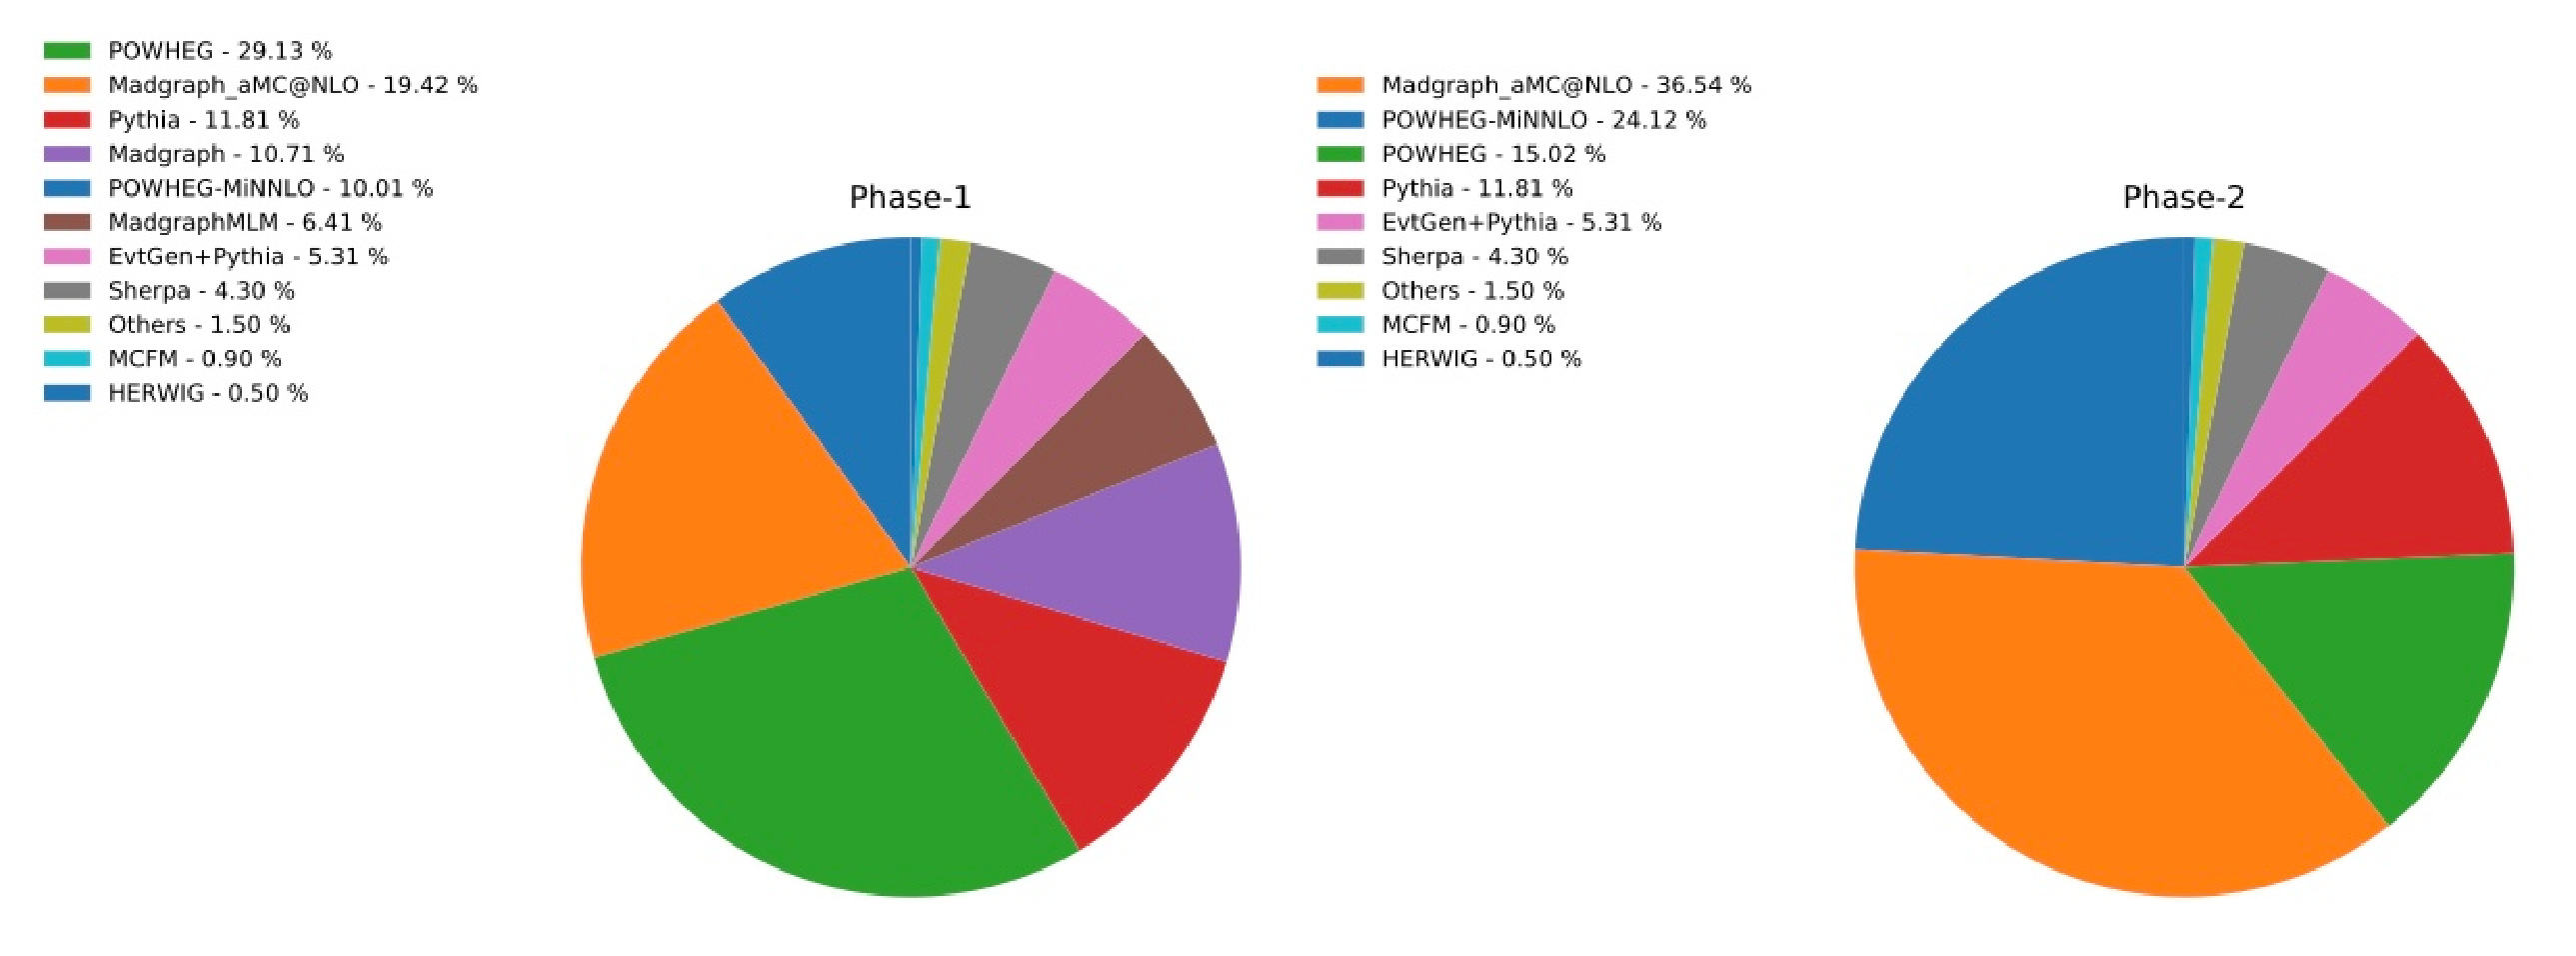
\includegraphics[width=16cm]{figs/6 Generators/generatorfraction_update.pdf} &
%\hspace{-0.1in}
%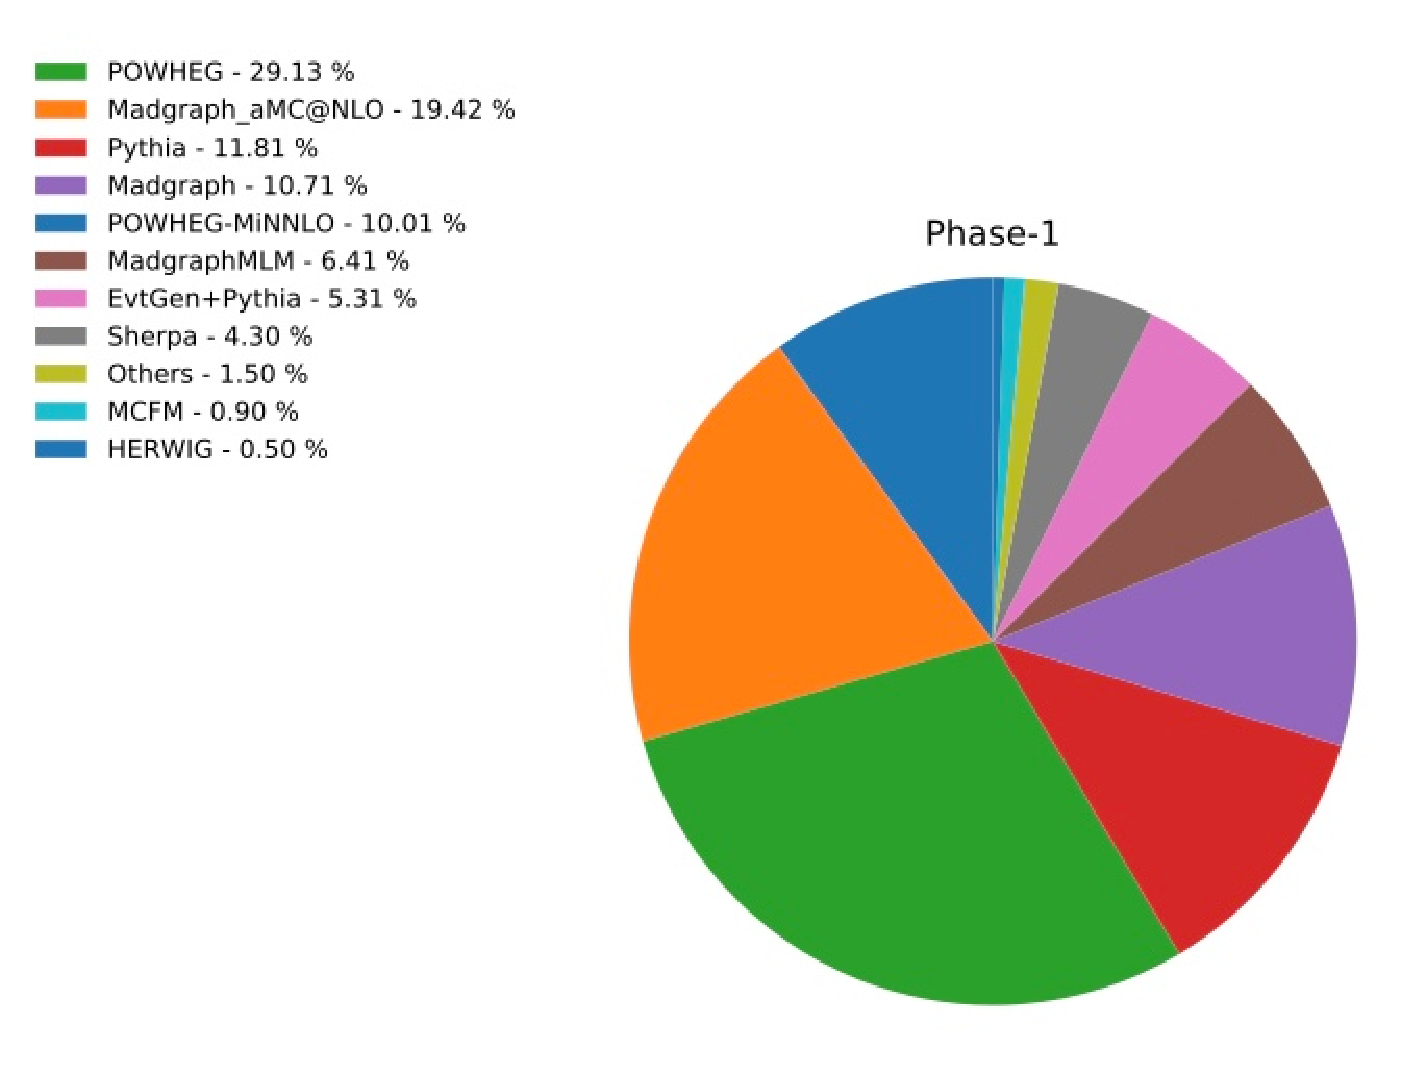
\includegraphics[width=8cm]{figs/6 Generators/generatorfraction_phase1_update.pdf} &
%\hspace{-0.2in}
%\vspace{0in}
%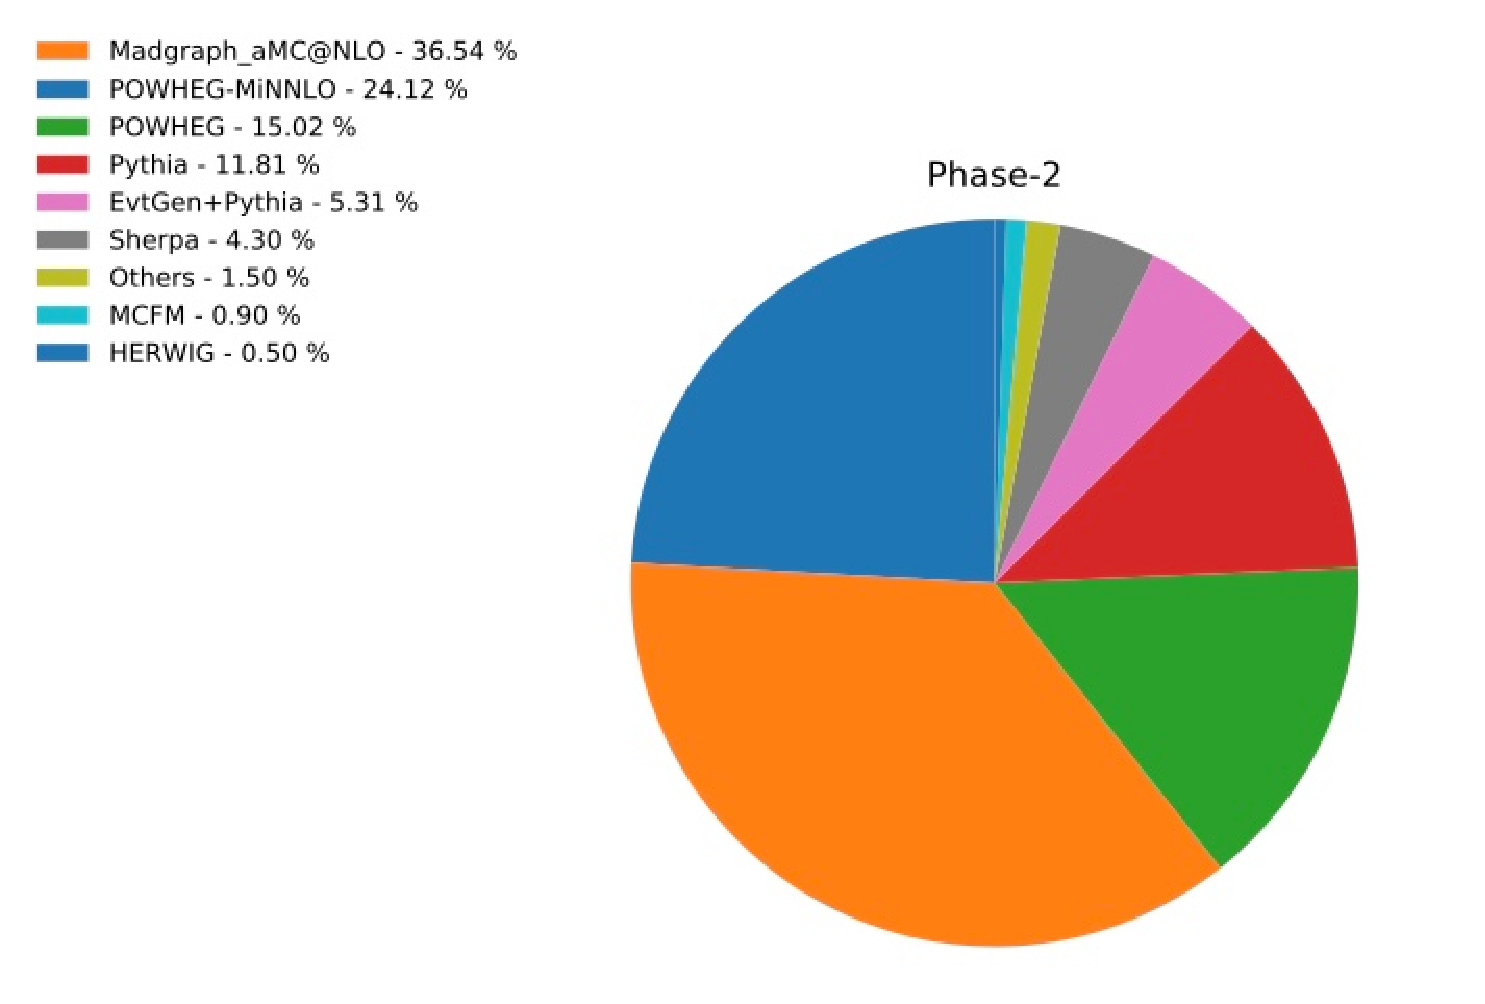
\includegraphics[width=8.5cm]{figs/6 Generators/generatorfraction_phase2_update.pdf}
% \end{tabular}
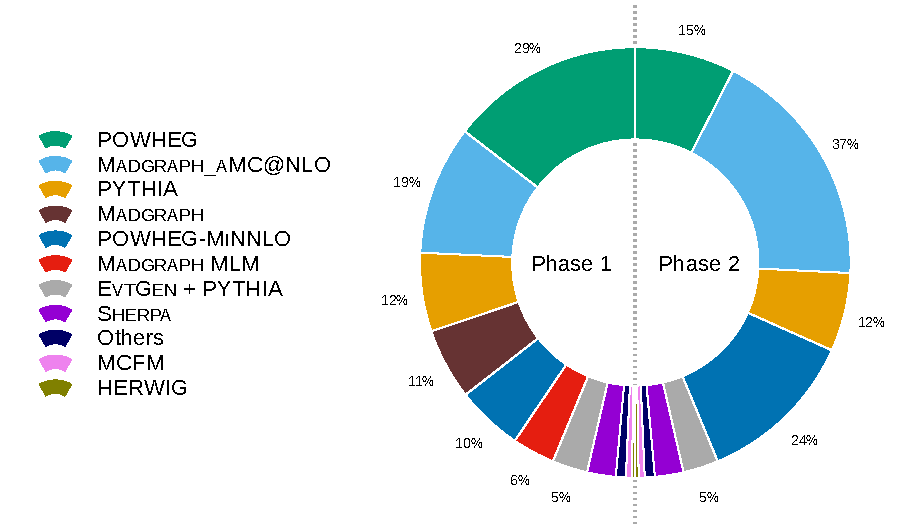
\includegraphics[width=.75\textwidth]{figs/6 Generators/out_gen_frac.pdf}
\caption{Usage of physics generators by CMS during \PhaseOne (left half) and expected usage during \PhaseTwo (right half), expressed as a fraction of the total events in each half of the plot.}
\label{fig:MCUsageComposition}
\end{figure}

\subsection{Time performance estimates}

Time performance benchmarks are based on workflows used to generate \PhaseOne simulated samples with current generator versions.
Since the generation step simulates the physics processes before the final-state particles enter the detector, the computational time does not depend on the detector geometry, the technical complexity of the upgraded detectors, nor the level of pileup. Table~\ref{tab:gen-timing} shows the \gls{CPU} time per event measured for different precision levels, as well as the fractions of events corresponding to each precision category. The bottom row shows the mean \gls{CPU} time per event for the \PhaseOne and \PhaseTwo generator mix. The pie charts in Fig.~\ref{fig:timeperevent} display the fraction of events produced (expected) at different levels of precision in perturbation theory in \PhaseOne (\PhaseTwo). It also shows the fraction of the total \gls{CPU} time spent on (projected for) event generation at different precision levels in \PhaseOne (\PhaseTwo). Note that the inclusion of NNLO processes in \PhaseOne was driven by the need for precise theoretical calculations of the $\PW$-boson production cross-sections and decays used in the \PW mass measurements.

\begin{table}[tbph]
    \centering
    \caption{Mean \gls{CPU} time per generated event for various levels of precision in perturbation theory, and fractions of events produced (projected) in each precision category for \PhaseOne (\PhaseTwo). The bottom row includes the mean \gls{CPU} time per generated event for the \PhaseOne and \PhaseTwo mix.}
    \begin{tabular}{|c|c|c|c|}
    \hline
    \rowcolor{tableheader} 
        Precision & \gls{CPU}/evt. & \multicolumn{2}{c}{Fraction of events} \\ 
    \rowcolor{tableheader} 
                  & HS23-s   & \PhaseOne    & \PhaseTwo    \\ \hline
    \cellcolor{tablerowheader}
        LO        &  150     & 36\%       & 14\%       \\ \hline
    \cellcolor{tablerowheader}
        LO (EvtGen) & 1\,500 & 5\%           & 5\%        \\\hline
    \cellcolor{tablerowheader}
        NLO       &  200     & 49\%       & 57\%       \\ \hline
    \cellcolor{tablerowheader}
        NNLO      &  1\,300   & 10\%       & 24\%       \\ \hline
    \rowcolor{tableheader} 
    \multicolumn{2}{c|}{Total \gls{CPU}/evt.}   & 356 HS23-s & 523 HS23-s \\ \hline
    \end{tabular}
    \label{tab:gen-timing}
\end{table}

\begin{figure}[!htb]
\centering
%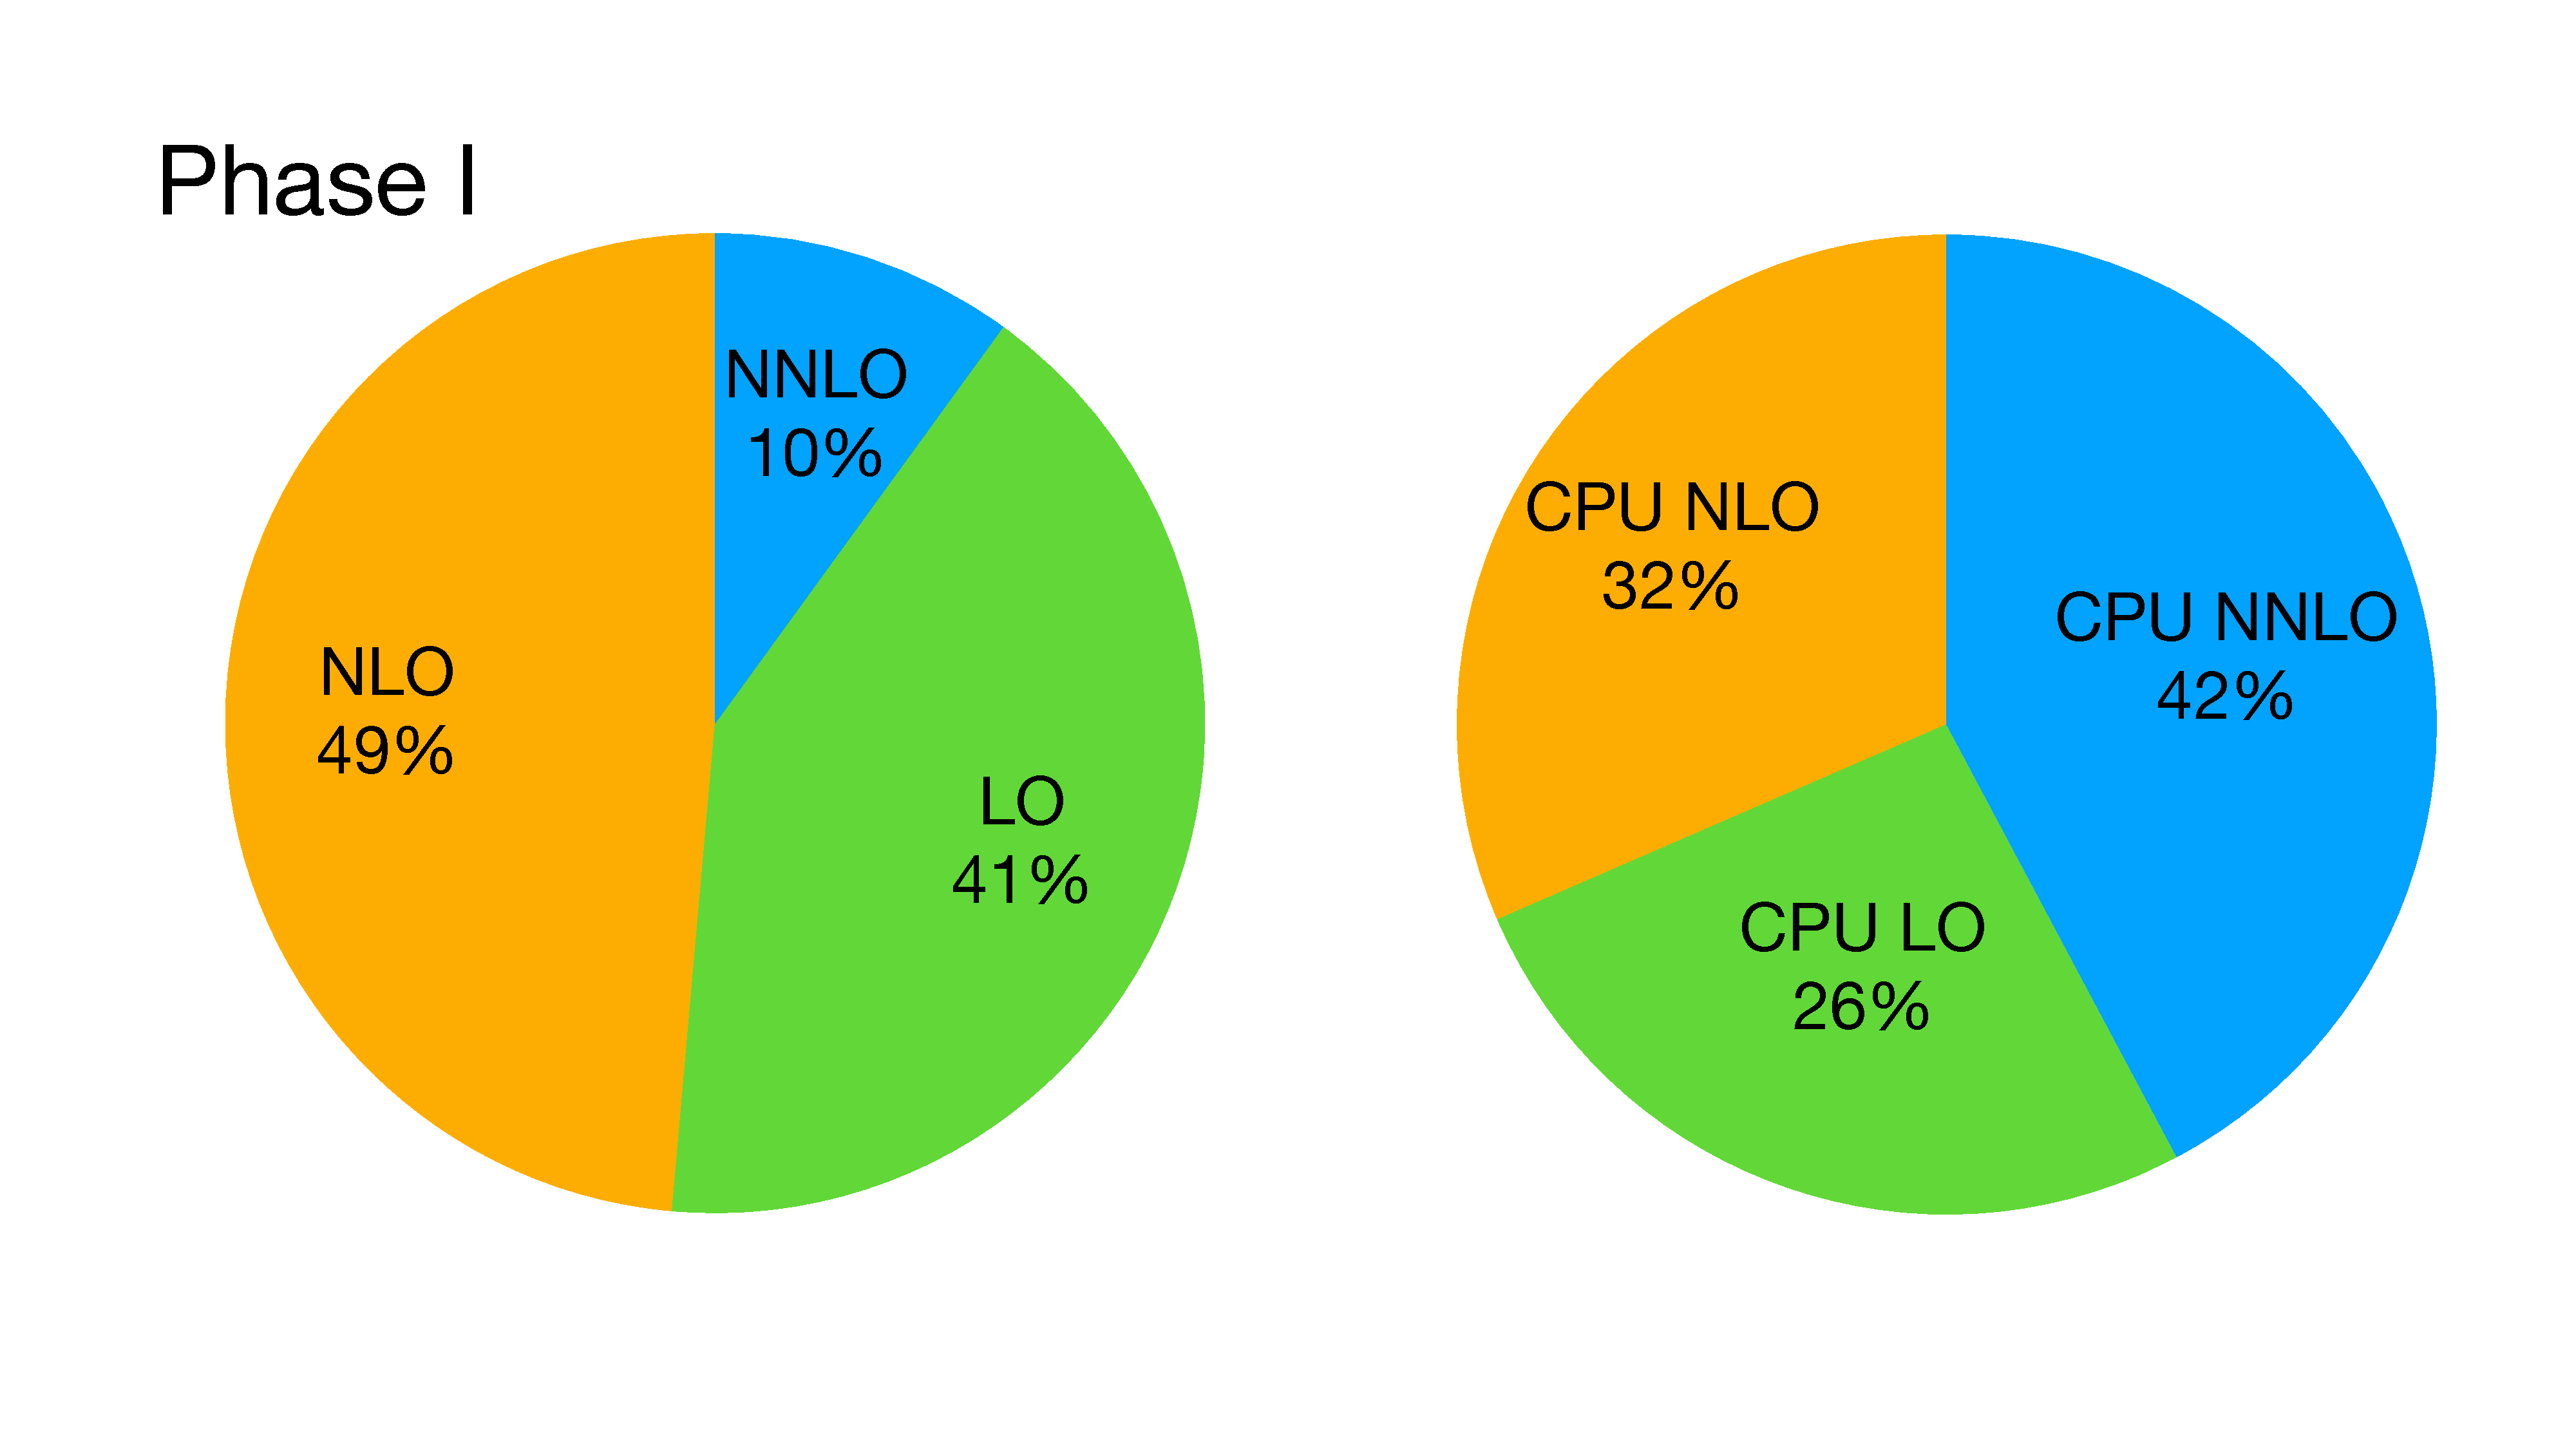
\includegraphics[width=12cm]{figs/generators/PhaseI_Plots.pdf}
%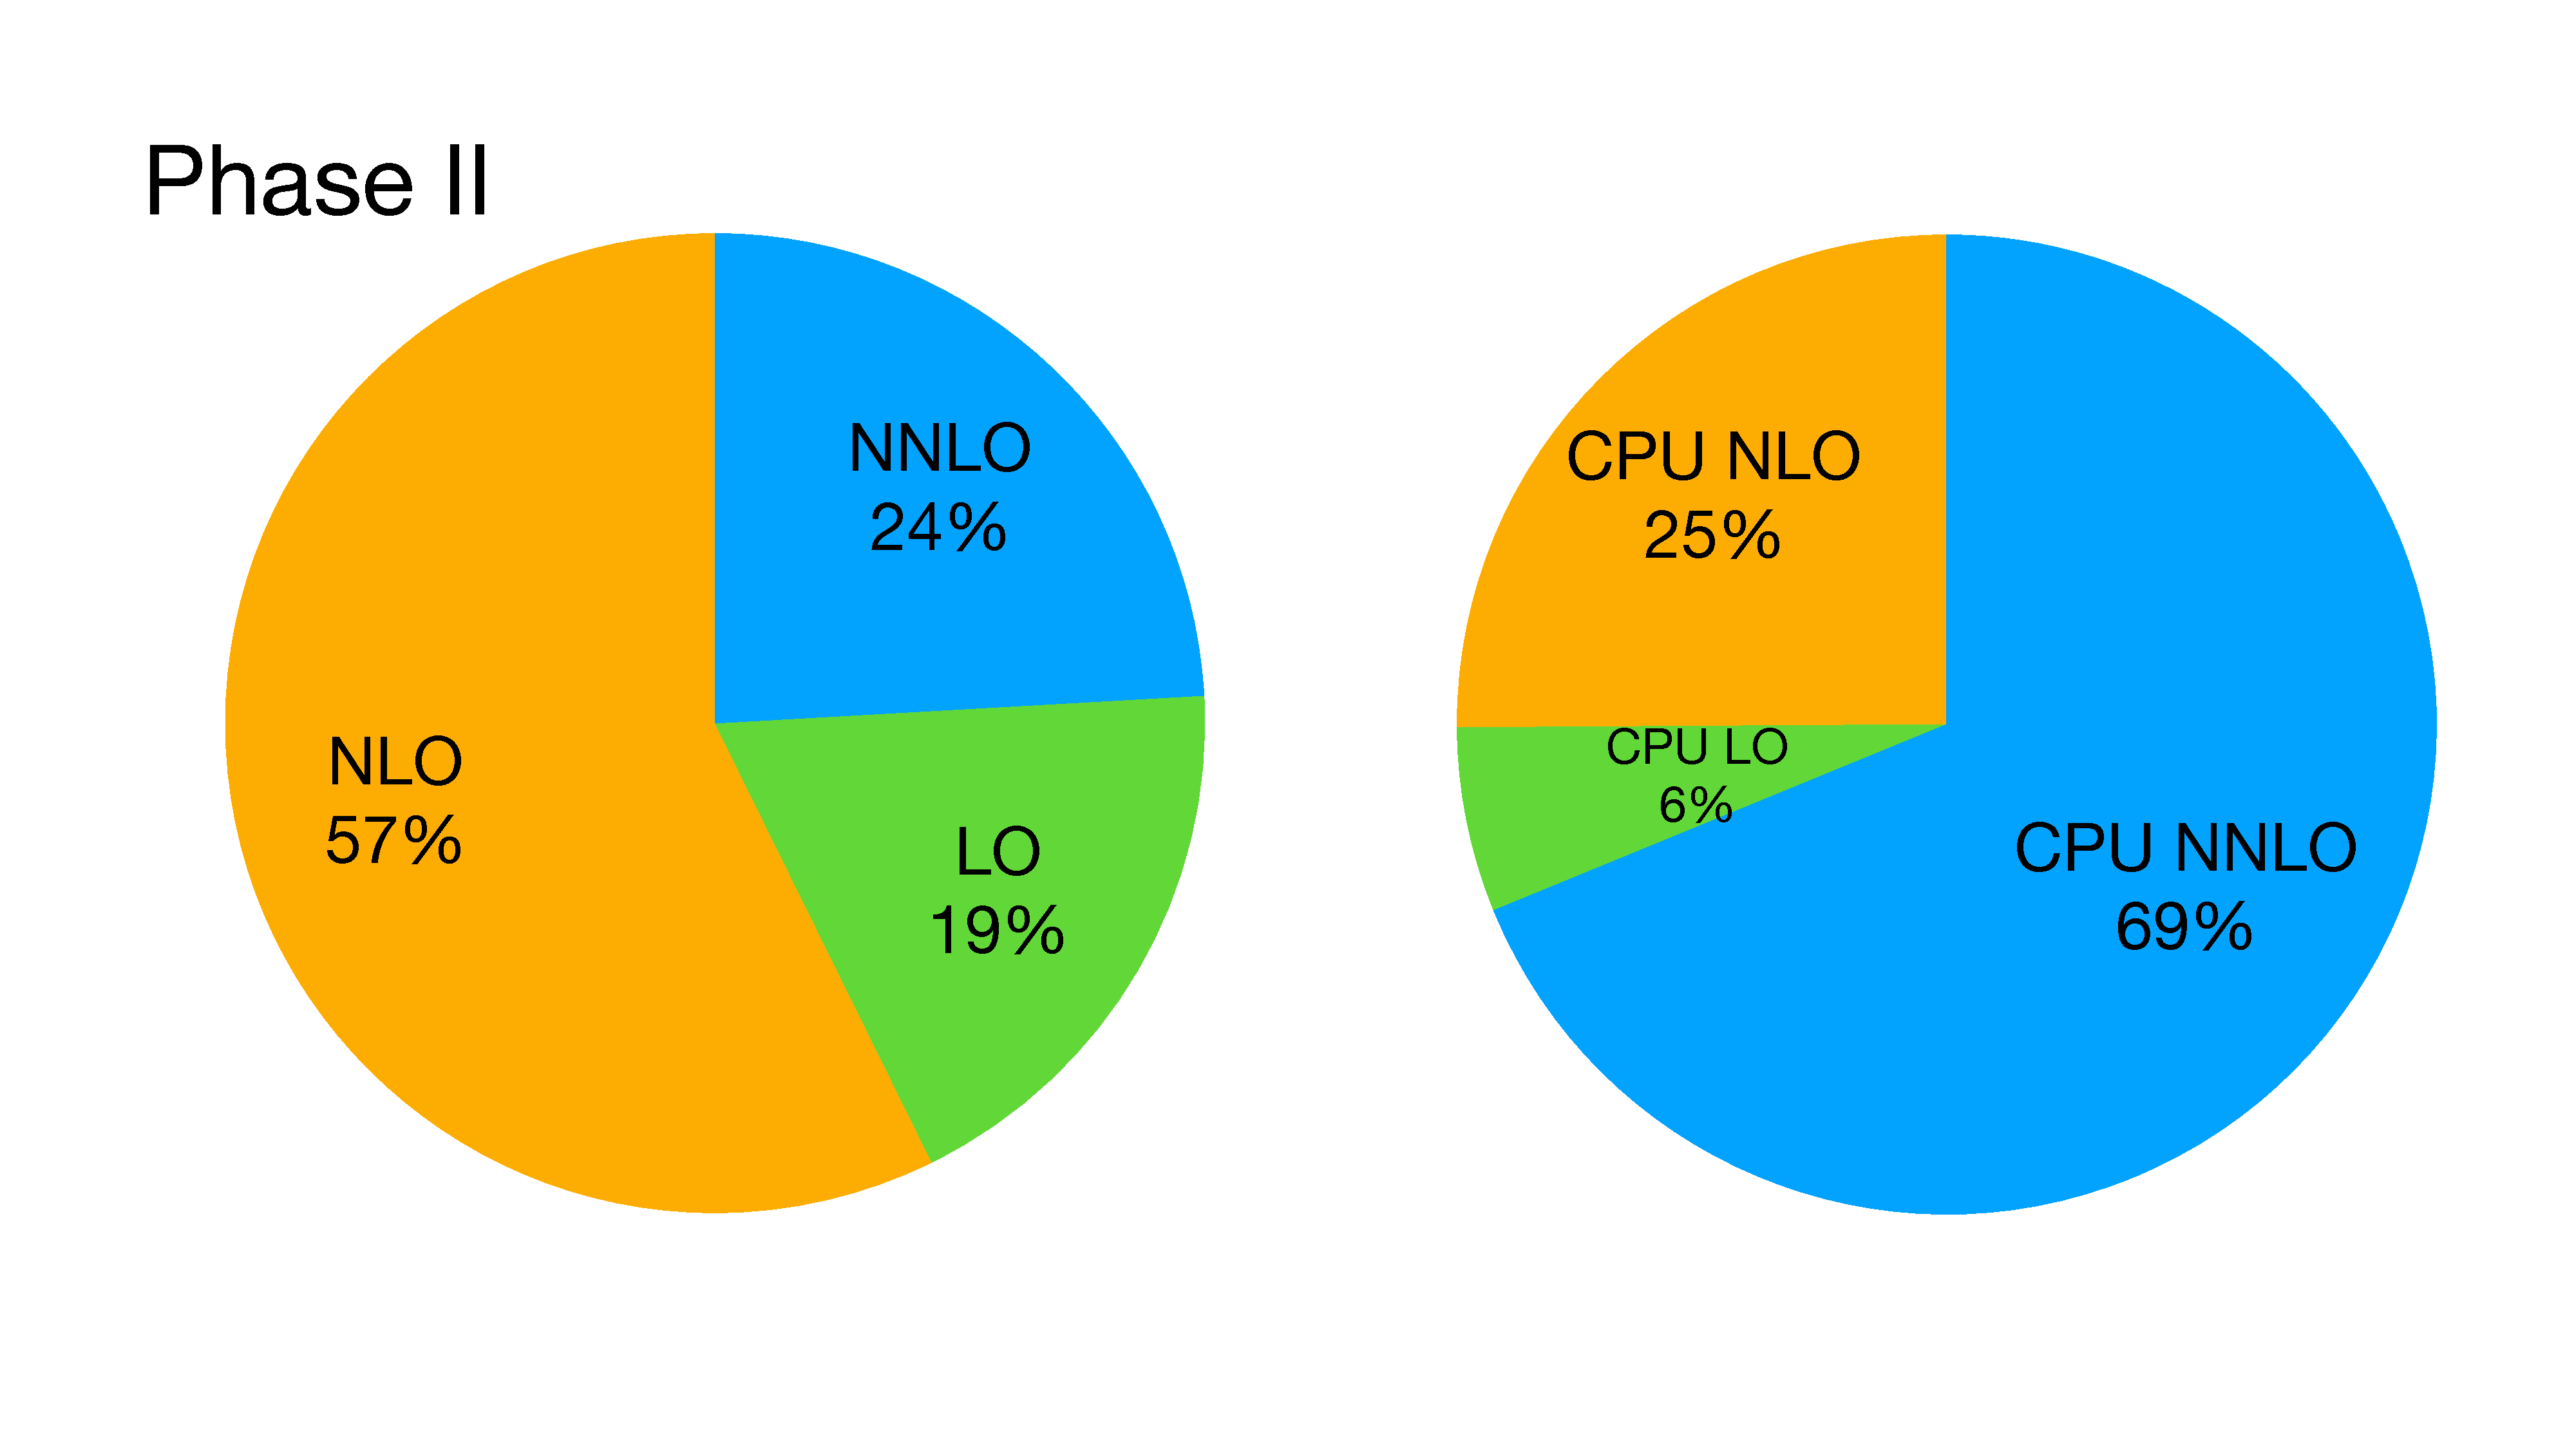
\includegraphics[width=12cm]{figs/generators/PhaseII_Plots.pdf}
% 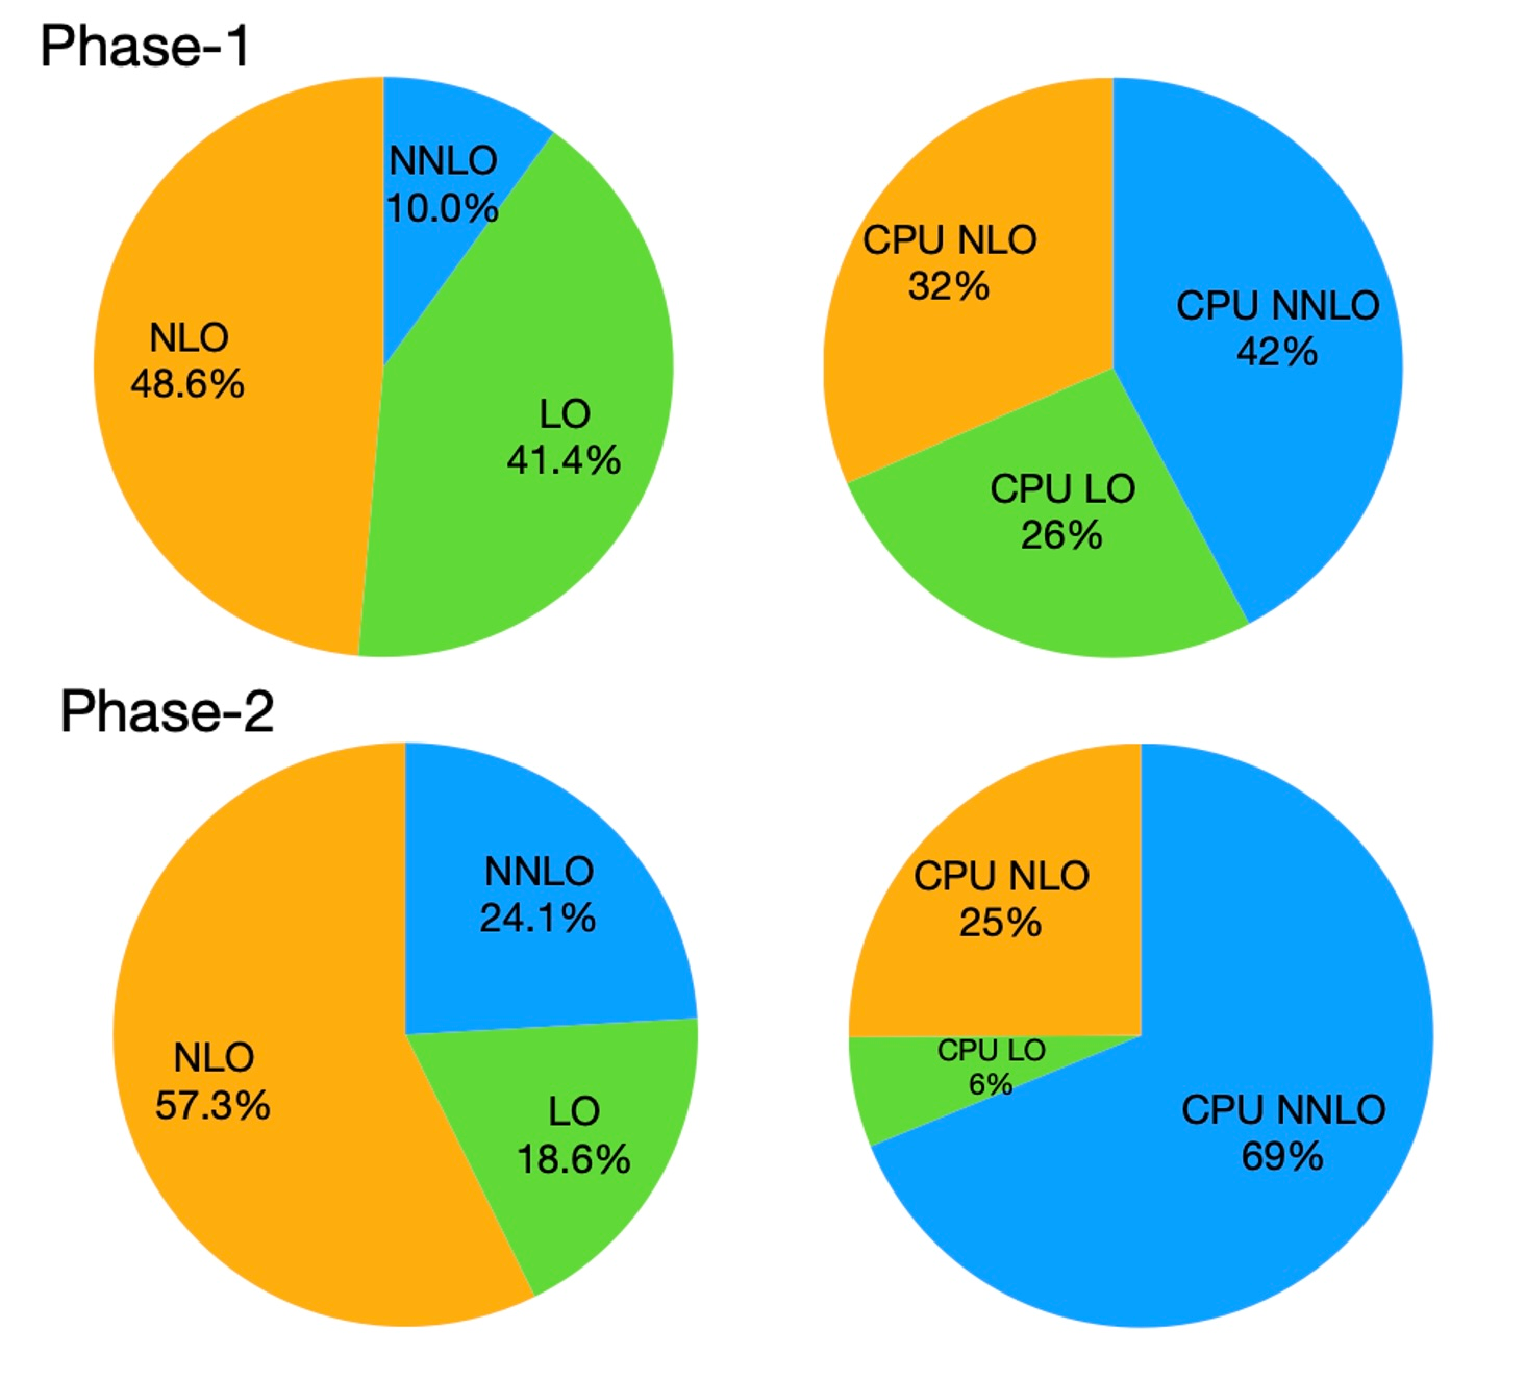
\includegraphics[width=12cm]{figs/6 Generators/Gen-Precision-Plots.pdf}
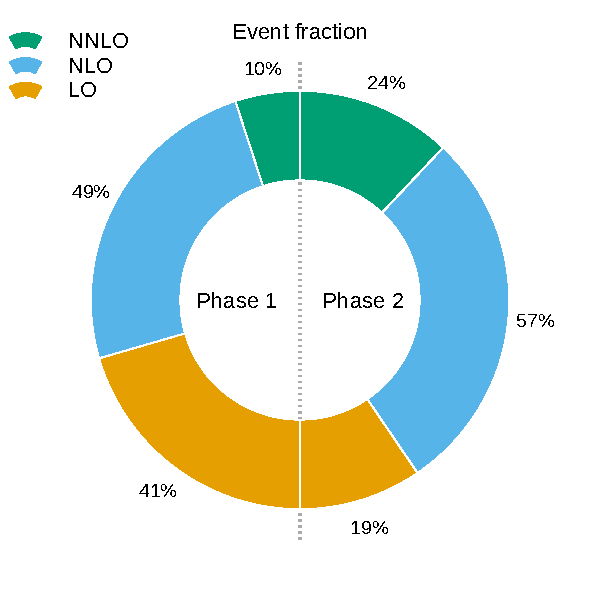
\includegraphics[width=0.45\textwidth]{figs/6 Generators/out_order_frac.pdf}
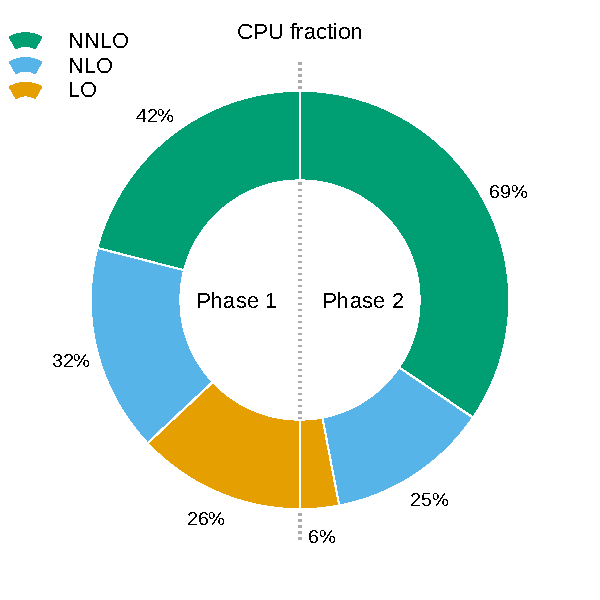
\includegraphics[width=0.45\textwidth]{figs/6 Generators/out_order_cpu_frac.pdf}
\caption{Fraction of generated events categorized by precision level in perturbation theory (left), and \gls{CPU} fraction utilized for each of these categories (right). The left halves of the charts represent the \PhaseOne generator mix, while the right halves illustrate the anticipated mix for \PhaseTwo.}
\label{fig:timeperevent}
\end{figure} 
\begin{figure}
\end{figure}


%\begin{table}[htb]
%\begin{center}
%\begin{tabular}{cc}
%\toprule
%Accuracy & HS06  \\
%\midrule
%{\cellcolor{blue!25} \gls{LO}} & {\cellcolor{blue!25} 150 } \\
%{\cellcolor{orange!25} \gls{NLO}} &  {\cellcolor{orange!25} 200}\\
%{\cellcolor{green!15} \gls{NNLO}} &  {\cellcolor{green!15} 1300}\\
%{\cellcolor{pink!25} N$^3$\gls{LO}} & {\cellcolor{pink!25} 13000}\\
%\hline\hline
%{\cellcolor{blue!05} Total time/event (\PhaseOne)} & {\cellcolor{blue!05} 289} \\
%{\cellcolor{blue!05} Total time/event (\PhaseTwo) } & {\cellcolor{blue!05} 456} \\
%{\cellcolor{blue!05} 152} \\
%{\cellcolor{blue!05} Total time/event (Phase \gls{II}) with $\alpha_s$ scaling} & {\cellcolor{blue!05}1847}\\%{\cellcolor{blue!05}1016} \\
%\bottomrule
%\end{tabular}
%\caption{\textcolor{cyan}{Mean \gls{CPU} time per event for various levels of precision in perturbative theory. The last two rows show the time per event computed as the mean for the generators mix used in \PhaseOne and the projected mix in \PhaseTwo.}}   
%\label{tab:time}
%\end{center}
%\end{table}


\subsection{R\&D to improve computing performance}
\label{sec:gen-rnd}

R\&D planning for generators includes projects external to CMS, carried out by generator development teams, as well as internal CMS activities. Some activities described in the following paragraphs aim to reduce \gls{CPU} time consumption by optimizing algorithms and code. In contrast, others aim to perform certain tasks with \gls{ML} or to offload computationally expensive tasks to \glspl{GPU}.

\subsubsection{Continuous improvements to event generators}

The \textbf{Gene.1} activity in Table~\ref{tab:gen-improvements} refers to the expectation of continuous code performance improvements of \gls{MC} generators used by CMS. Most of these developments are external to CMS and performed by the generator theory community. To estimate the \gls{CPU} time performance improvement per year for an average event in the CMS generators mix, the assumptions are that usage or time performance improvements to high-precision generators other than \textsc{Madgraph\_aMC@NLO} are negligible and that \textsc{Madgraph\_aMC@NLO} will continue to improve at the 6\% per year level measured by CMS during the last four years. For example, since the matrix element computation is the most compute-intensive part of a generator workflow, the expected 20--30\% total reduction in \textsc{PYTHIA} \gls{CPU} time per event through the start of \RunFour would have a negligible effect in the generator mix.
These assumptions yield a 2\% per-event-per-year time performance improvement for the CMS generator mix, as presented in Table~\ref{tab:gen-improvements}.

\subsubsection{Optimization of CMS-specific generators code}

The \textbf{Gene.2} activity in Table~\ref{tab:gen-improvements} refers to improvements and optimization of CMS-specific code. In particular, one activity aims to reduce \textsc{POWHEG}-\textsc{MiNLO}'s \gls{CPU} consumption by removing some of the \gls{PDF} choices available in the generated samples.
\textsc{POWHEG}-\textsc{MiNLO} is expected to be the most compute expensive generator in \PhaseTwo, and the only generator with a \gls{ME} computation for each different \gls{PDF} set. The reduction in the number of \gls{PDF} choices in \textsc{POWHEG}-\textsc{MiNLO} would lower \gls{CPU} needs by approximately 20\%, yielding a one-time 15\% \gls{CPU} time improvement for the average event in the generators’ mix.

\subsubsection{Negative weights in NLO calculations}
\label{sec:Negative}

Negative weights are a severe source of inefficiency in \gls{MC} event generation. They are an artifact of the matching scheme of partons produced through \gls{NLO} calculations with parton showers, such as those modeled in \textsc{Madgraph\_aMC@NLO}. If $f_{\text{neg}}$ is the fraction of negatively contributing events, a factor of~$\frac{1}{(1-2\times f_{\text{neg}})^2}$ more events will need to be produced to compensate. As mentioned in Section~\ref{sec:rnse}, the fraction of events with negative weights in \textsc{Madgraph\_aMC@NLO} \ttbar production~\cite{NegWeight}, $f_{\text{neg}}=23\%$, is taken as an upper limit of $f_{\text{neg}}$ for the \PhaseTwo physics process mix generated with \textsc{Madgraph\_aMC@NLO}.

The \textbf{Gene.3} activity in Table~\ref{tab:gen-improvements} aims to mitigate the deleterious effect of negatively weighted events for the generation of processes relevant to CMS. It refers to R\&D within the generator theory community~\cite{Andersen:2023cku, Andersen:2021mvw, Shyamsundar:2025arcane}, based on a technique that removes negatively weighted events by redistributing weights without biasing observables. Success of this effort would reduce the number of events produced with \textsc{Madgraph\_aMC@NLO} by a factor of~3.4~\cite{NegWeight}, bringing the fraction of \textsc{Madgraph\_aMC@NLO} events from 37\% (Fig.~\ref{fig:MCUsageComposition}) to 15\%.
%for generating the average event in the \PhaseTwo mix. Other than Madgraph\_aMC@NLO, \gls{NLO} events are produced with \textsc{POWHEG}, which, by design, does not produce negatively weighted events, \textsc{Sherpa}, and other generators.

\subsubsection{Code vectorization and porting to \gls{GPU}}

Physics generator teams, e.g.,  \textsc{Madgraph\_aMC@NLO} and \textsc{Sherpa}, are working to adapt their code to run on \glspl{GPU}. The authors of \textsc{Madgraph\_aMC@NLO} plan to deliver a fully vectorized version on time for \gls{HL-LHC}. They have demonstrated that efficient vectorization of matrix element computation would enable the calculation of complex processes on \glspl{GPU}. The vectorized code, when run on \glspl{CPU}, would speed up these physics generators by a factor of~3. The impact on the average event in the \PhaseTwo generators mix would be approximately 15\% (\textbf{Gene.4} in Table~\ref{tab:gen-improvements})

In addition to code vectorization, the \textbf{Gene.4} activity in Table~\ref{tab:gen-improvements} also refers to R\&D to port and offload generator tasks to \glspl{GPU}. Using a \gls{GPU}- compatible version of \textsc{Madgraph\_aMC@NLO} would yield a time performance improvement of several orders of magnitude for tasks offloaded to \glspl{GPU}~\cite{madgraph4gpu1, madgraph4gpu2, madgraph4gpu3}. \textsc{Madgraph} authors estimate that 80--95\% (50--70\%) of the \gls{CPU} time spent on \gls{LO} (\gls{NLO}) \gls{ME} calculations would be offloaded to \glspl{GPU}. A 30--45\% effective reduction in generation time for the average generated event in the \PhaseTwo mix is to be expected from \textsc{Madgraph} and \textsc{Sherpa} task offloading to \glspl{GPU}. It must be noted that the source of this potential time savings is not algorithm re-engineering that would yield a time performance gain per (\gls{CPU}) node, but would come at the expense of adding \gls{GPU} computing resources. The CMS generator group will adopt a co-development model, actively collaborating with the generator theory community to integrate, test, and validate the \gls{GPU} prototypes as they become available.

\subsubsection{Machine learning algorithms}

The \textbf{Gene.5} activity in Table~\ref{tab:gen-improvements} refers to the potential introduction of neural network techniques to calculate the matrix elements in the event generation process. The options under consideration are based on an end-to-end \gls{ML} approach to event generation. The neural network method shows favorable time scaling with additional partons~\cite{Moodie:2022flt, Aylett-Bullock:2021hmo}, where numerical calculations with state-of-the-art tools are insufficient. 
%The specific problem of diphoton production~\cite{Moodie:2022flt, Aylett-Bullock:2021hmo} arising from gluon fusion offers unique challenges associated with infrared divergences from soft and collinear emissions, where a naive neural network model struggles and an ensemble is used with one network for each divergent structure of the process. 
While this work is exploratory, it shows that the generator theory community is actively seeking creative solutions to circumvent the most \gls{CPU}-intensive part of the event generation workflow. If successful, these \gls{ML}-based methods would allow the elimination of the need to perform the matrix element calculations. By offloading close to 90\% of the inference \gls{CPU} time to \glspl{GPU}, the time per event for the event generation step would be negligible with respect to the rest of the simulation chain. 
Other areas in which \gls{ML} techniques may be used are the unweighting procedure to transform generator outputs to closely resemble those observed  in the detector. The latter is explored for processes with high parton multiplicity~\cite{gen5, Danziger:2021eeg}, which would yield speed-up factors of up to 10. The use of \gls{ML} techniques for the hadronization step is also under study~\cite{Ilten:2022jfm} in the context of the \textsc{PYTHIA} event generator.

\begin{table}[tbph]
    \centering
    \caption{Summary of generator-related R\&D activities with estimated impacts and probabilities of success on the timescale of the beginning of \RunFour. \gls{CPU} time savings or offloaded to \glspl{GPU} are expressed as a fraction of the total \gls{GEN} time.}
    \begin{tabular}{|c|c|c|c|}
    \hline
    \rowcolor{tableheader} 
           &                               &                            & Prob. of \\ 
    \rowcolor{tableheader}
           & Description                   &       Impact               & Success or \\  
    \rowcolor{tableheader}
           &                               &                  (Fraction of total GEN CPU time)          & Adoption   \\ \hline
    \cellcolor{tablerowheader}
  Gene.1   &  {Continuous improvements}    &  {2\% CPU speed-up}         &   High   \\
    \cellcolor{tablerowheader}
           &   {to event generators}       &      { (Per year)}         &          \\ \hline
    \cellcolor{tablerowheader}
  Gene.2   &   {Optimizations of CMS-specific} &  {15\% one time CPU savings} &   High   \\
    \cellcolor{tablerowheader}
           &   {generators code}           &   {(Removal of PDF choices)}&          \\ \hline
    \cellcolor{tablerowheader}
  Gene.3   &   {Eliminate Negatively}      &  {3.4 times less \textsc{Madgraph}-NLO events}                   &  Medium   \\
\cellcolor{tablerowheader}       &    {weighted events}                           &  Reduction from 37\% to 15\% of total &   \\ \hline
    \cellcolor{tablerowheader}
  Gene.4   &  Code vectorization and       &  {15\% one time CPU savings}  &   High  \\
    \cellcolor{tablerowheader}
           & offload to GPU                &  {(Avg. event in mix on CPU)}   &          \\ 
               \cellcolor{tablerowheader}
           &    &    &   \\
    \cellcolor{tablerowheader}
           &    &   {80--95\% LO \textsc{Madgraph} CPU }      &   {High} \\ 
    \cellcolor{tablerowheader}
           &    &   {time offloaded to GPU}      &   \\ 
    \cellcolor{tablerowheader}
           &    &    &   \\
    \cellcolor{tablerowheader}
           &    &   {50--70\% NLO \textsc{Madgraph} CPU }      &   {Medium} \\
     \cellcolor{tablerowheader}
           &    &   {time offloaded to GPU}      &   \\
           \hline
    \cellcolor{tablerowheader}
  Gene.5   &   {ML for expensive} &   {90\% inference CPU time} & Low     \\
    \cellcolor{tablerowheader}
           &   {generator tasks (e.g., MEs)}  &   {offloaded to GPU} &         \\ \hline
    \end{tabular}
    \label{tab:gen-improvements}
\end{table}

\clearpage

%%%%%%%%%%%%%%%%%%%%%%%%%%%%%%%%%%%%%%%%%%%%%%%%%%%%%%%%%%%%%%%%%%%%%%%%%%%%%%%%
%
% DETECTOR SIMULATION
%
%%%%%%%%%%%%%%%%%%%%%%%%%%%%%%%%%%%%%%%%%%%%%%%%%%%%%%%%%%%%%%%%%%%%%%%%%%%%%%%%
% \clearpage
% \input{tex/06_detector_simulation.tex}
\section{Detector simulation}
\label{sec:Simulation}

Detector simulation is essential to \gls{HEP} collaborations as a tool to accomplish different goals, such as making the physics case for an experiment, designing detector components, developing and optimizing software algorithms, stress-testing computing infrastructure, developing methods for data analysis, and interpreting the results in the context of theoretical calculations. The development of detector simulation tools is a large-scale community effort~\cite{HEPSoftwareFoundation:2018fmg,Apostolakis:2022nnf}.

Two primary software applications for detector simulation are in production during \PhaseOne. \textbf{Full simulation (\textsc{FullSim})}~\cite{Lange:2015sba, Hildreth:2015kps, Hildreth:2017vpw, CMS:2021dly, Srimanobhas:2024nmy} begins with a  \GEANTfour-based module~\cite{GEANT4:2002zbu,Allison:2016lfl} that simulates particle transport and interaction with matter (``\gls{SIM}'' step), followed by a second module to model the electronic signal (``\gls{DIGI}'' step). In CMS, the \textsc{FullSim} application benefits from numerous technical improvements and physics-preserving approximations that allow it to run more than five times faster than \GEANTfour with default settings~\cite{Pedro:2018jqu,Srimanobhas:2024nmy}. A ``MIXING'' step overlays the pileup interactions at the \gls{DIGI} level. The last step in the \textsc{FullSim} chain is standard reconstruction, which uses the same algorithms as in real data.

\textbf{Fast simulation (\textsc{FastSim})}~\cite{Sekmen:2016iql} uses parametric modeling and fast reconstruction algorithms, achieving a 10--20 speed-up over \textsc{FullSim}. The speed-up increases with pileup multiplicity~\cite{CMS-DP-2023-063}, and most physics observables are modeled within a 10\% accuracy.
\textsc{FastSim} is part of \gls{CMSSW} and provides a complete simulation of low-level objects (hits and clusters) tuned to match \textsc{FullSim}. Pileup is modeled in \textsc{FastSim} in the same way as in \textsc{FullSim}, with the exception that tracks, rather than tracker \gls{DIGI} objects, are mixed together.
Tracking reconstruction is accelerated by using generator-level information rather than standard algorithms, while other reconstruction sequences are preserved.

In addition to \textsc{FullSim} and \textsc{FastSim}, machine learning approaches are being explored. Generative \gls{ML} (\textbf{ML4Sim}) may be employed to replace or augment specific simulation components to increase the \textsc{FullSim} processing speed while maintaining output quality (\textbf{\textsc{MLFullSim}}), or to increase the \textsc{FastSim} output quality while maintaining the processing speed (\textbf{\textsc{MLFastSim}}). Separately, \textbf{an ultra-fast approach, \textsc{FlashSim}}~\cite{Vaselli:2024hml}, uses \gls{ML} to directly generate end-stage event products for analysis (NanoAOD), based on event-level input information. The fraction of \PhaseTwo simulation generated with any of these approaches is still to be determined.

This section describes how the CMS geometry model and simulation applications will evolve towards \gls{HL-LHC}, as well as R\&D activities to improve computational performance while maintaining or improving the physics fidelity of the simulation.

\subsection{Evolution of the geometry model}

The detector geometry and material descriptions are core components of particle transport modeling. Detector Description for \gls{HEP} (\textsc{DD4hep})~\cite{Gaede:2020tui}, a community-developed detector description software tool initially targeting future collider studies, was adopted by CMS in \RunThree and is already utilized to model the \PhaseTwo CMS detector. Input parameter values are stored in and read from \gls{XML} files and used to build both the \textsc{FullSim} and reconstruction geometries; \textsc{FastSim} uses a simplified version of the \textsc{FullSim} geometry and the same reconstruction geometry. \textsc{DD4hep} enables the construction of internal model representations independent of the geometry modeler back-end and provides interfaces for importing geometry representations from many sources~\cite{Vuosalo:2020bwn, CMS:2021dly}.

\subsection{Electronic signal simulation and pileup event mixing}

Pileup interactions, representing multiple hard interactions taking place either within the same bunch crossing (in-time), or in neighboring bunch crossings (out-of-time), deserve their own section, given their impact on \PhaseTwo reconstruction computing performance. The pileup contribution is added to the signal event by the mixing module~\cite{Lange:2015sba}. \textsc{FullSim} or \textsc{FastSim} simulated hits are grouped into readout channels to construct a \gls{DIGI} object, which includes the electronic signal modeling. The signal-plus-pileup event overlay is performed at the \gls{DIGI} level for both \textsc{FullSim} and \textsc{FastSim}.

There is a ``classical'' approach to event overlay, used in \RunOne, and a ``premixing''~\cite{Hildreth:2017vpw} approach, which was used in \RunTwo and \RunThree, and will be optimized for \gls{HL-LHC}. In classical mixing, pileup interactions are read from a sample of simulated minimum-bias events and added to the signal event one by one, resulting in a high I/O cost; the method worked well in \RunOne but does not scale in \RunTwo. As pileup increases, the network’s read rate to obtain the required minimum-bias events per signal event grows too rapidly. Instead, premixed pileup libraries are prepared in advance and contain single events that are an overlay of a predetermined number of minimum-bias events, with each event representing ``pure pileup'' at a given instantaneous luminosity. 
Premixed events are stored in a custom, digitized format for compression, which requires specific development for each subdetector system.
This circumvents the need to handle a large number of input files of minimum-bias events for pileup simulation. It scaled well into \RunThree, reducing I/O by 90\% and the \gls{CPU} time required to digitize and reconstruct events by a factor of~2 relative to classical mixing. 
However, the size of the premixed input samples grew to O(10\unit{PB}) due to increasing pileup and the number of detector channels from the \PhaseOne upgrades, requiring limits on the fraction of these samples hosted on disk.

\subsection{Time performance estimates for \textsc{FullSim} and \textsc{FastSim}}

Table~\ref{tab:fullsim_time_per_event} shows a measurement of the time it takes to process a \ttbar event through the \PhaseTwo \gls{SIM} (\GEANTfour) and \gls{DIGI} steps, taken as an estimator of the average processing time per event for the generator mix. As noted before, the \gls{SIM} time does not depend on the number of pileup interactions because their contributions are added later in the chain.
The premixed pileup library is produced once and reused for all samples in a given simulation campaign, so the computing time to produce it is effectively amortized and therefore not included here.

Table~\ref{tab:fastsim_time_per_event} compares all \gls{MC} simulation production steps for \textsc{FullSim} and \textsc{FastSim} using the \PhaseOne configuration, which is the latest currently available in \textsc{FastSim}. Note that the time for the \gls{SIM} step is reduced by a factor of~75 with respect to \textsc{FullSim}.

\begin{table}[tbhp]
    \centering
	\caption{Estimated average time per event for the simulation steps using \textsc{FullSim} with the \PhaseTwo detector configuration for various \gls{PU} scenarios.
	All estimates are derived in \gls{CMSSW}\_14\_0\_X by processing 500 events across four threads on a dedicated machine with all cores fully loaded, yielding a per-core HS23 score of 14.55. Values marked with * are estimated via linear interpolation from the surrounding values.}
    \begin{tabular}{|r|r|r|}
    \hline
    \rowcolor{tableheader} 
    $\langle \text{PU} \rangle$         & SIM (HS23) & DIGI (HS23) \\ \hline
    \cellcolor{tablerowheader} 0        & 543        & 132 \\
    \cellcolor{tablerowheader} * 100    & 543        & 350 \\
    \cellcolor{tablerowheader} 140      & 543        & 433 \\
    \cellcolor{tablerowheader} * 150    & 543        & 460 \\
    \cellcolor{tablerowheader} * 180    & 543        & 526 \\
    \cellcolor{tablerowheader} 200      & 543        & 573 \\
    \hline
    \end{tabular}
	\label{tab:fullsim_time_per_event}
\end{table}

\begin{table}[tbhp]
    \centering
	\caption{Estimated average time per event for \textsc{FullSim} (upper) and \textsc{FastSim} (lower) for all steps using the \PhaseOne detector configuration for various \gls{PU} scenarios. All estimates are derived in \gls{CMSSW}\_14\_0\_X by processing 500 events across four threads on a dedicated machine with all cores fully loaded, yielding a per-core HS23 score of 14.55. \textsc{FullSim} is limited to lower pileup values due to limitations in the \PhaseOne tracker. Values marked with * are estimated via linear (\gls{DIGI}) or quadratic (\gls{RECO}) interpolation from the surrounding values.}
    \begin{tabular}{|r|r|r|r|r|}
    \multicolumn{5}{c}{FullSim}\\
    \hline
     \rowcolor{tableheader} 
     $\langle \text{PU} \rangle$   & SIM (HS23) & DIGI (HS23) & RECO (HS23) & Total (HS23) \\ \hline
     \cellcolor{tablerowheader} 0  & 249        & 29          & 21          & 299 \\
     \cellcolor{tablerowheader} 20 & 249        & 66          & 63          & 378 \\
     \cellcolor{tablerowheader} 40 & 249        & 105         & 141         & 495 \\
     \cellcolor{tablerowheader} 60 & 249        & 144         & 282         & 675 \\
    \hline
    \multicolumn{5}{c}{\textsc{FastSim}}\\
    \hline
    \rowcolor{tableheader} 
    $\langle \text{PU} \rangle$    & SIM (HS23) & DIGI (HS23) & RECO (HS23) & Total (HS23) \\ \hline
    \cellcolor{tablerowheader}   0   & 3.1        & 13          & 12          & 28.1 \\
    \cellcolor{tablerowheader}   20  & 3.1        & 23          & 23          & 49.1 \\
    \cellcolor{tablerowheader}   40  & 3.1        & 33          & 38          & 74.1 \\
    \cellcolor{tablerowheader}   60  & 3.1        & 43          & 53          & 99.1 \\
    \cellcolor{tablerowheader}   80  & 3.1        & 55          & 74          & 132.1 \\
    \cellcolor{tablerowheader}   100 & 3.1        & 64          & 98          & 165.1 \\
    \cellcolor{tablerowheader}   140 & 3.1        & 82          & 165         & 250.1 \\
    \cellcolor{tablerowheader} * 150 & 3.1        & 86          & 187         & 250.1 \\
    \cellcolor{tablerowheader} * 180 & 3.1        & 101         & 254         & 250.1 \\
    \cellcolor{tablerowheader}   200 & 3.1        & 108         & 304         & 415.1 \\
    \hline
    \end{tabular}
\label{tab:fastsim_time_per_event}
\end{table}

\subsection{R\&D to improve physics models and computing performance}
\label{sec:RDDetSim}

%The accuracy of the physics models in \GEANTfour was not a limiting factor to the precision and sensitivity of most CMS physics measurements during \PhaseOne~\cite{HEPSoftwareFoundation:2018fmg}. 

The \GEANTfour module within the CMS full simulation workflow uses more than 30\% of the total CMS \gls{CPU} allocation in \RunThree. In itself, this fact calls for the \GEANTfour Collaboration to undertake an ambitious R\&D program to reduce \gls{CPU} consumption while preserving its physics performance.
The emphasis of the \PhaseTwo physics program on precision measurements demands, however, improvements to the \GEANTfour physics models, a requirement that is computationally expensive. Improving physics models is particularly important to fully exploit the novel materials and high granularity of the \gls{HGCAL}~\cite{CMS:2019MIPTDR, Apostolakis:2022nnf}. Furthermore, the increase in complexity and granularity of the CMS \PhaseTwo detector adds a high computational cost to geometry modeling and particle propagation in the simulation. CMS responds to this challenge with an R\&D plan for \PhaseTwo that includes continuous optimization of algorithms and code, the use of \gls{ML} tools, and the porting of simulation tasks to \glspl{GPU}. 

During \RunTwo, approximately 13\% of simulation events were produced using \textsc{FastSim}, while the rest were produced using \textsc{FullSim}. \textsc{FastSim} was primarily used to produce signal samples for supersymmetry (SUSY) searches. 
Ongoing R\&D activities therefore target improvements in the physics accuracy of \textsc{FastSim} to make it capable of delivering 50--75\% of the total number of simulation events used in analysis without loss of precision or sensitivity in the measurements. \gls{ML} techniques may play a significant role in helping CMS to achieve this goal.
% The break-down of \gls{MC} events requested by PAG is shown in Figure~\ref{fig:simple}. 
%As of today, the CMS physics organization reports that the \RunThree physics program can be carried out with a negligible loss in precision or reach with up to 50\% of the needed Monte Carlo events produced via FastSim 
%The upper limit projected for \gls{HL-LHC}, dependent on the success of activities to improve FastSim physics accuracy, is 75\%. 
%In a scenario where FlashSim R\&D evolves into a tool that achieves a physics performance comparable to FastSim, a fraction of these events may be produced with FlashSim in \RunFour.
%where not only sustainability goals could be achieved, but also an increase in the quantity of interpretation material provided by analyses. 

In a scenario where successful R\&D evolves \textsc{MLFullSim}, \textsc{MLFastSim}, and/or \textsc{FlashSim} into a tool that delivers physics performance comparable to or better than \textsc{FastSim}, a fraction of the simulation events may be produced with these \gls{ML}-based simulations in \RunFour, reducing the consumption of computing resources even further.
\textsc{MLFullSim}, if sufficiently accurate, would be used for almost all \textsc{FullSim} production.
\textsc{MLFastSim} would increase the \textsc{FastSim} fraction from the initial 50\% target up to 75\%.
\textsc{FlashSim} is expected to be used for 25\% of events, primarily for signal models and minor backgrounds, where only NanoAOD-level variables would be needed.

\subsubsection{Incremental improvements to \GEANTfour physics and software}

The \textbf{Simu.1} activity in Table~\ref{tab:sim-improvements} is external to CMS and would result in a 5\% annual reduction in the \gls{CPU} time per event, while achieving the goal to improve physics capabilities. This conservative estimate is based on \GEANTfour's benchmarking studies as a function of release version using a CMS standalone application. The \GEANTfour Collaboration plans to continue delivering versions of the toolkit every year with incremental improvements to physics and software. Following a co-development model with the \GEANTfour team, CMS timely integrates, tests, and validates the latest \GEANTfour releases~\cite{CMS:2021dly} within \gls{CMSSW}. 

\subsubsection{Optimization of the CMS \GEANTfour-based module}

The \textbf{Simu.2} activity in Table~\ref{tab:sim-improvements} represents CMS internal efforts to achieve a projected 50\% \gls{CPU} time performance gain in the \gls{CMSSW} \GEANTfour module through the adoption and optimization of the latest software compilers, algorithm improvements, and physics-preserving approximations~\cite{Hildreth:2015kps, Srimanobhas:2024nmy}. As an example, the \textbf{Simu.1} and \textbf{Simu.2} activities combined delivered a 40\% decrease in the \gls{CPU} time per event in the 2019--2024 period, as illustrated in Fig.~\ref{fig:SIM-timing}.

\begin{figure}[tbh]
    \centering
    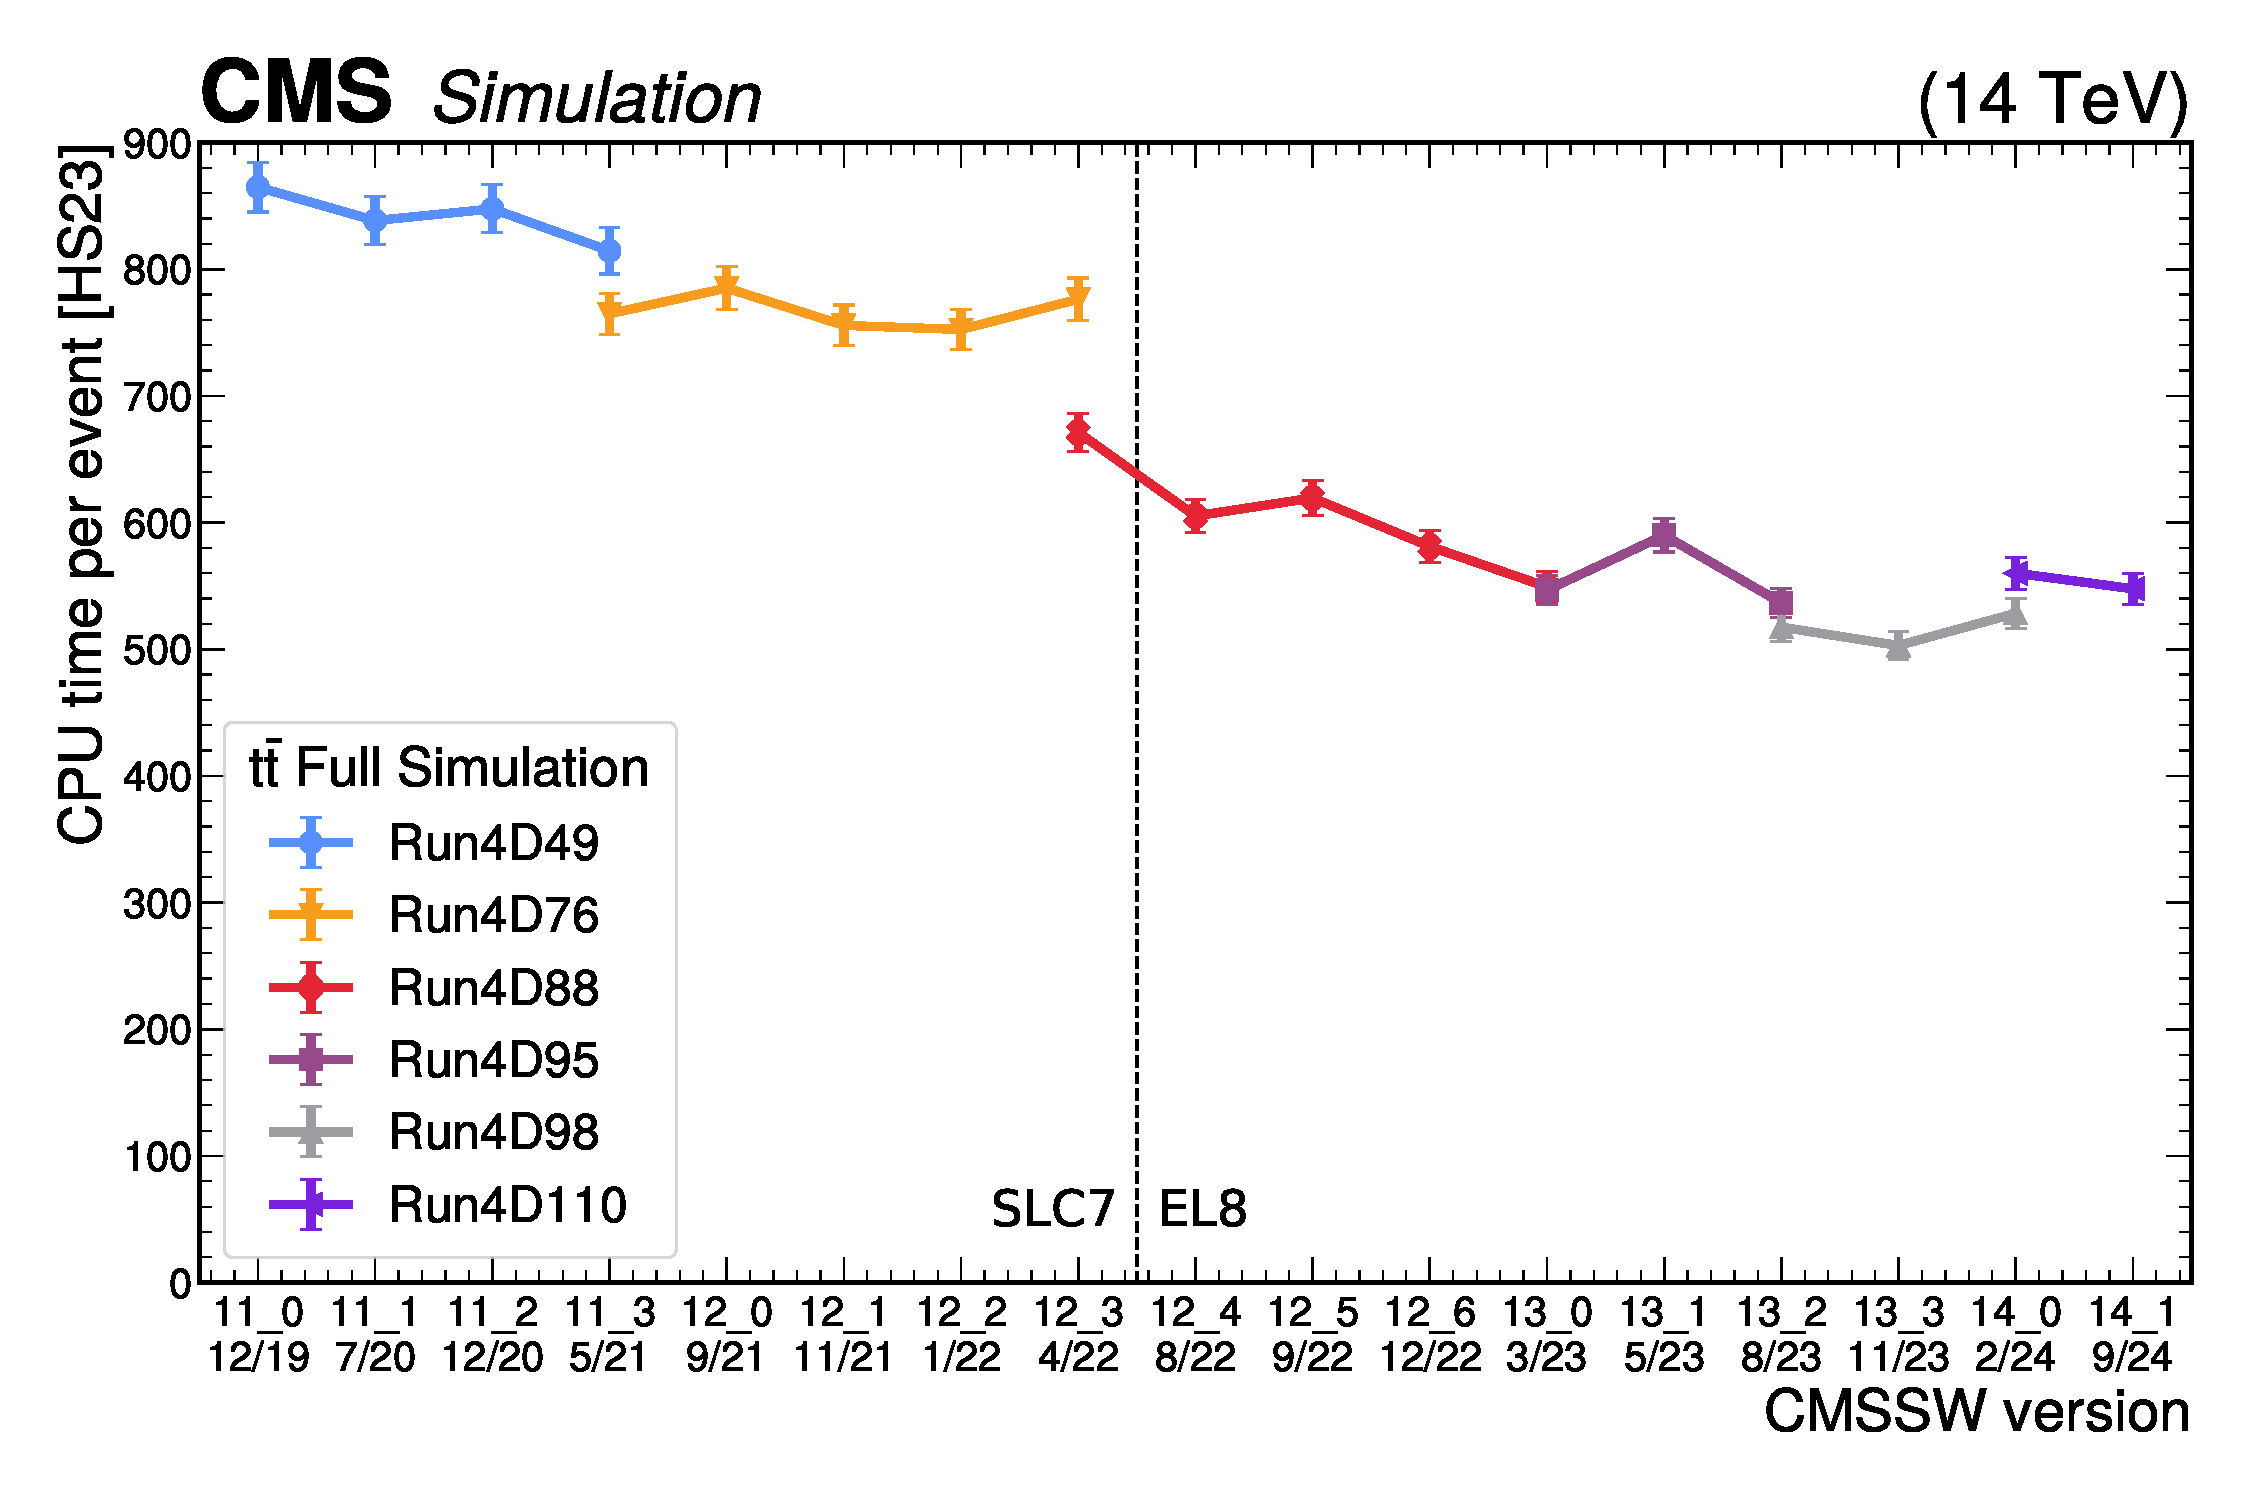
\includegraphics[width=1\textwidth]{figs/7 Simulation/Summary_Plots_CMSSW_history_CPU_time_SIM_1_thread_phase-2_FullSim_v4b.pdf}
    \caption{Improvement in the \PhaseTwo timing per event (arbitrary units) for the \GEANTfour-based module of \textsc{FullSim} from 2019 to 2024. The legend denotes different simulated versions of the \PhaseTwo detector upgrades, with more realistic geometries as the ``D'' number increases.}
    \label{fig:SIM-timing}
\end{figure}

\subsubsection{Offload \GEANTfour tasks to \glspl{GPU}}
\label{sec:SimulationGeant4GPU}
 Porting selected \GEANTfour tasks to \glspl{GPU} requires intensive R\&D efforts by external collaborations and by CMS. Two research teams, AdePT~\cite{Amadio:2022mqi} and Celeritas~\cite{Johnson:2024qqt}, are working within \GEANTfour to achieve the goal. The \textbf{Simu.3} activity in Table~\ref{tab:sim-improvements} describes the effort to offload \GEANTfour \gls{EM} shower simulation to \glspl{GPU} at the start of \RunFour. This task accounts for 50--75\% of the \gls{CPU} time associated with the \gls{SIM} step. \textbf{Simu.4} in Table~\ref{tab:sim-improvements} refers to the goal to offload neutron interactions, in addition to \gls{EM} showers, to \glspl{GPU} by the start of \RunFive. The amount of code offloaded would represent 75--95\% of the \gls{CPU} time of the \gls{SIM} step. Although these activities are the responsibility of teams external to CMS, the experiment needs to invest effort in early integration, testing, and validation of evolving prototypes.

\subsubsection{Event mixing for pileup modeling}

The size of the premixed pileup library is driven by the complexity of the events and scales with the pileup and the number of simulation events required for the most significant tasks, to avoid event duplication. Both the premixed sample and the minimum-bias sample used to build it must be at least 2.5 times larger than the event sample used in a physics analysis. Given the large size of these libraries, they are hosted only in the largest storage systems, e.g., at CERN and \gls{FNAL}, and data is served remotely to simulation workflows at nearby sites. Optimizing the size of these libraries is an active area of R\&D  with potential implications for disk storage requirements (\textbf{Simu.10} in Table~\ref{tab:sim-improvements}).

Alternatively, CMS may explore generating and simulating the minimum-bias (MinBias) events used for pileup mixing on the fly, rather than precomputing MinBias samples as done for both classical mixing and premixing. This would lead to two increases in the \gls{CPU} usage of the \gls{DIGI} step: the additional \gls{GEN}-\gls{SIM} step for $n_{\text{MinBias}} = n_{\text{BX}}n_{\text{\gls{PU}}}$ MinBias events per signal event (where $n_{\text{BX}}$ is the number of bunch crossings), and the return to classical mixing rather than premixing, where more simulated hits must be processed per event (as opposed to premixing, where the processing of simulated MinBias hits is amortized because the premixed library is prepared in advance).
Table~\ref{tab:on_the_fly_pileup} provides inputs to estimate the \gls{CPU} impact from both sources.
The scaling of classical mixing with pileup is approximately a factor of three worse than premixing.
The \PhaseTwo simulation currently includes three out-of-time bunch crossings on either side, so $n_{\text{BX}} = 7$ and $n_{\text{MinBias}} = 980\text{--}1\,400$ for $n_{\text{\gls{PU}}} = 140\text{--}200$. Three scenarios are considered but not \textsc{FullSim} MinBias, which is prohibitive even with \gls{GPU} simulation engines:
\begin{enumerate}
\item \textsc{FastSim} MinBias: the \gls{CPU} time in the \gls{DIGI} step would increase by a factor of~11--13 for signals simulated with the \PhaseTwo \textsc{FullSim} (bounded by the \textsc{FastSim} \PhaseOne performance and the extrapolated \PhaseTwo performance). Optimizations may be found to reduce this increase. The physical validity of the output will also need to be confirmed, as the quality of \textsc{FastSim} tracker hits for this purpose has not been studied.
\item Premix \gls{GEN}: as an intermediate option, noting that the generator uses 90\% of the total \gls{GEN}-\gls{SIM} time for MinBias events in the \textsc{FastSim} case, the generator output (HepMC) particles, 25\unit{kB/event}) could be premixed, with just the \textsc{FastSim} \gls{SIM} step running on the fly to provide simulated hits for mixing. This would lead to only a factor of~4.4 increase in the \gls{DIGI} step \gls{CPU} time, while reducing the disk usage of premixed samples by more than a factor of~10.
\item \gls{ML} MinBias: the generative models in Section~\ref{subsubsec:genml} target a particular detector and simulate each particle independently. For the MinBias pileup simulation, a model conditioned only on $n_{\text{\gls{PU}}}$ would have constant-time inference scaling. Hits would need to be generated for every subdetector, beyond the \gls{HGCAL}-oriented case in Section~\ref{subsubsec:genml}. A sufficiently sophisticated model, able to learn details such as the tracker alignment on a per-event basis, could potentially be trained on data, actually improving the physical validity of the pileup simulation. This is the best option in terms of \gls{CPU} time, especially if the model inference is performed on \gls{GPU}; however, it also requires the most R\&D.
\end{enumerate}
While this approach necessarily entails some additional computational time, it would largely or entirely eliminate the disk and network usage of the premixing approach. This resource trade-off will need to be carefully considered, depending on the convergence of either of the R\&D approaches above (\textsc{FastSim} or generative \gls{ML}). This activity is summarized as \textbf{Simu.12} in Table~\ref{tab:sim-improvements}.

\begin{table}[htbp]
    \centering
	\caption{Upper: the \gls{GEN}-\gls{SIM} time per MinBias event for different simulation engines and detector configurations. The \textsc{FastSim} \PhaseTwo value, marked with *, is extrapolated from the other values in the table (noting that 90\% of the \RunThree value is \gls{GEN}). Middle: the classical mixing time for \textsc{FullSim} with different detector configurations and pileup values. Lower: the same for premixing (from Tables~\ref{tab:fullsim_time_per_event} and~\ref{tab:fastsim_time_per_event}). The scaling of classical mixing with pileup can be seen to be roughly a factor of~3 worse than classical mixing, consistently for both \PhaseOne and \PhaseTwo.}
    \begin{tabular}{|r|r|r|}
    \multicolumn{3}{c}{MinBias}\\
    \hline
     \rowcolor{tableheader} 
     Type & Phase & GEN-SIM (HS23) \\ \hline
     \cellcolor{tablerowheader} \textsc{FullSim} & 1 & 51\hphantom{.5*} \\
     \cellcolor{tablerowheader} \textsc{FullSim} & 2 & 94\hphantom{.5*} \\
     \cellcolor{tablerowheader} \textsc{FastSim} & 1 & 4\hphantom{.5*} \\
     \cellcolor{tablerowheader} \textsc{FastSim} & 2 & 4.5* \\
    \hline
    \end{tabular}\\
    \begin{tabular}{|r|r|r|r|}
    \multicolumn{4}{c}{Classical mixing (\textsc{FullSim})}\\
    \hline
    \rowcolor{tableheader} 
    $\langle \text{PU} \rangle$ & Phase & DIGI (HS23) & Slope (HS23/\gls{PU}) \\ \hline
    \cellcolor{tablerowheader} 0   & 1 & 29   & \NA \\
    \cellcolor{tablerowheader} 60  & 1 & 445  & 6.9 \\
    \cellcolor{tablerowheader} 0   & 2 & 132  & \NA \\
    \cellcolor{tablerowheader} 140 & 2 & 1\,090 & 6.8 \\
    \hline
    \multicolumn{4}{c}{Premixing (\textsc{FullSim})}\\
    \hline
    \rowcolor{tableheader} 
    $\langle \text{PU} \rangle$ & Phase & DIGI (HS23) & Slope (HS23/\gls{PU}) \\ \hline
    \cellcolor{tablerowheader} 0   & 1 & 29  & \NA \\
    \cellcolor{tablerowheader} 60  & 1 & 144 & 1.9 \\
    \cellcolor{tablerowheader} 0   & 2 & 132 & \NA \\
    \cellcolor{tablerowheader} 140 & 2 & 433 & 2.1 \\
    \hline
    \end{tabular}
\label{tab:on_the_fly_pileup}
\end{table}

\subsubsection{DIGI step offloaded to \glspl{GPU}}
The \gls{DIGI} step processes the parameters needed to model signal smearing, cross-talk, dead channels, and calibration. A challenge for \gls{HL-LHC} is the management of the large memory load caused by the new \gls{MTD} detector and the large number of \gls{HGCAL} channels.
Porting the \gls{DIGI} step to \glspl{GPU} also offers an excellent opportunity to increase event throughput, because the code is amenable to vectorization with instances of single instructions applied to multiple \gls{DIGI} objects. The success of the \textbf{Simu.11} activity in Table~\ref{tab:sim-improvements} would allow for up to 50\% of the \gls{DIGI} \gls{CPU} time to be offloaded to \glspl{GPU}.

%In parallel with the development and optimization of the \GEANTfour-based FullSim application, there is the development and use of the Fast Monte Carlo chain, or ''FastSim''. FastSim is part of the \gls{CMSSW} core framework and provides a complete simulation of low-level objects (hits and clusters) tuned to match FullSim. FastSim also performs reconstruction and production of high-level modules, such as those for identifying leptons and jets.

\subsubsection{Incremental physics improvements in \textsc{FastSim}}

Work is needed to update the geometry representations in \textsc{FastSim} to account for the new detectors in the \PhaseTwo upgrade. The geometry and particle-interaction models for the \PhaseTwo tracker, \gls{MTD}, \gls{GEM}, and \gls{HGCAL} are currently under development using the modular framework for detector geometry in \textsc{FastSim}, with the aim of converging by the end of \RunThree. This work also incorporates incremental upgrades that will improve the physics fidelity and increase the number of simulation events that can use \textsc{FastSim}, from the current \RunFour baseline of none (\textbf{Simu.5} in Table~\ref{tab:sim-improvements}).
%For example, dedicated pixel resolution histograms for the Phase-1 and Phase-2 tracker implementations will improve tracking and vertexing accuracy in FastSim. 
%Efficiency and resolution effects seen for high-\pt tracks ($\pt>1100\GeV/c$) will be addressed, allowing FastSim to be used by \PZpr-related analyses.  

\subsubsection{\textsc{FastSim} accuracy improvements with ML}
The \textbf{Simu.6} activity in Table~\ref{tab:sim-improvements} pursues the use of \gls{ML} methods to improve the accuracy of \textsc{FastSim} with respect to \textsc{FullSim}. The goal is to achieve a physics fidelity level that allows 50\% of the simulated samples to be produced with \textsc{FastSim} without compromising the quality of CMS physics measurements. In one of the leading approaches, identical event samples corresponding to various physics processes are generated and independently fed into the Full and fast simulation production workflows. The final collections in \textsc{FastSim} are then regressed using neural networks on an object-by-object basis to better match the equivalent \textsc{FullSim} objects~\cite{Banerjee:2022gkg,Bein:2023ylt,NIPS1987_a87ff679}. A large sector of analysis-level variables should be covered by the start of \RunFour, with the difference between \textsc{FastSim} and \textsc{FullSim} reduced to levels as low as 1--5\%.
%A recent prototype~\cite{bib:moritz} has been trained using the modified differential method of multipliers~\cite{NIPS1987_a87ff679} to learn the optimal combination of multiple loss terms enforcing both per-event and ensemble accuracy. This dramatically improves the accuracy of the DeepJet flavor-tagging observables and their correlations with each other and with other jet-based observables, reducing the FastSim-FullSim differences from 10\% to 1\% or less. It may be possible to extend the idea of refinement to the lower-level simulated hits, further improving the accuracy of FastSim, as initially explored in~\cite{Banerjee:2022gkg}. Our plan is to expand this approach to cover a large sector of NanoAOD variables in time for readiness during Run 3.

\subsubsection{Generative ML model for \gls{HGCAL} offloaded to \glspl{GPU}}
\label{subsubsec:genml}
Generative \gls{ML} models (\textbf{Simu.7} in Table~\ref{tab:sim-improvements}) can entirely replace either \textsc{FullSim} or \textsc{FastSim} components, leading to \textsc{MLFullSim} or \textsc{MLFastSim} applications as hybrids of the existing classical techniques and \gls{ML}.
The primary motivation is to achieve fast, accurate simulation of the \gls{HGCAL}, which is the most time-consuming \PhaseTwo subdetector.
Generative \gls{ML} can be deployed on \gls{GPU} to accelerate its inference, leading to substantially faster particle shower simulation than \GEANTfour, even for large \gls{ML} models.
Generative \gls{ML} may also achieve accuracy at the 1\% level, higher than that of a classical \textsc{FastSim} approach that uses a simplified geometry and parametrized shower models. Numerous possibilities are currently under investigation~\cite{Adelmann:2022ozp,Hashemi:2023rgo}, including the standard taxonomy of generative adversarial networks (GANs)~\cite{Scham:2023usu}, variational autoencoders (VAEs), and normalizing flows (NFs)~\cite{Schnake:2024mip}, as well as newer architectures such as diffusion models~\cite{Amram:2023onf,Buhmann:2023kdg} and autoregressive transformers.
%The ease of development and maintenance, computing performance, and physics accuracy for MLFullSim and MLFastSim remain to be assessed and should be compared to higher-level augmentations of the CMS FastSim (\textbf{Simu.6} above).
Optimistically, it is expected that \textsc{MLFullSim} could be accurate enough to replace nearly all classical \textsc{FullSim} usage. At the same time, \textsc{MLFastSim} could be accurate enough to be used for up to 75\% of events (likely in combination with \textbf{Simu.6}).
%In particular, graph-based message passing~\cite{Kansal:2021cqp} or point clouds~\cite{Buhmann:2023bwk}, as well as other geometric adaptation techniques, are being developed to handle the \gls{HGCAL} geometry, which does not neatly fit into the regular grid data formats used by industry generative \gls{ML}.

%Another alternative would be directly interfacing \gls{ML} algorithms with \GEANTfour; the ease of development and maintenance, computing performance, and physics accuracy of this approach, compared to augmentations of the CMS FastSim, remain to be assessed. In either case, \gls{ML} algorithm inference can naturally be accelerated on GPUs (see \textbf{Simu.10} in Table~\ref{tab:sim-improvements}, providing another path to exploit new computing resources for more efficient simulation.

\subsubsection{ML-based \textsc{FlashSim} physics fidelity}

Machine learning algorithms would be employed to transform generator-level physics events into final data products usable in analyses by directly mapping generator-level objects to analysis-level NanoAOD collections. 
If successful, the \textbf{Simu.8} activity in Table~\ref{tab:sim-improvements} could deliver physics accuracy similar to \GEANTfour-based \textsc{FullSim} with orders of magnitude speed-up. 
%If FlashSim is successful (e.g., by demonstrating optimal physics performance already in Run 3), 
The target goal would be to replace 25\% of events, half of the 50\% \textsc{FastSim} events, by \textsc{FlashSim} events at the start of \RunFour.
This target is motivated by the percentage of simulation events, estimated from \RunThree, for specific searches (signals and minor backgrounds) that could be conducted using only NanoAOD-level variables.
The \textbf{Simu.9} activity in Table~\ref{tab:sim-improvements} acknowledges the fact that \gls{ML} algorithm inference can naturally be accelerated on \glspl{GPU}.

\subsection{Summary of detector simulation-related R\&D activities} 

The relative computational and physics performance of \textsc{FullSim}, \textsc{FastSim}, and \textsc{FlashSim} will ultimately determine their future utilization proportions. Adoption of \textsc{FastSim} during \RunTwo was at the 13\% level in terms of the numbers of events, mainly to model signal samples associated with \gls{BSM} searches. The baseline scenario for \RunFour is to use \GEANTfour-based \textsc{FullSim} for all simulation needs and to incorporate fast simulation options when their physics accuracy makes them suitable.

Table~\ref{tab:sim-improvements} lists the various detector simulation R\&D activities discussed in this chapter. The list includes estimates of the potential impacts on the physics fidelity, code performance, or resource requirements. Our estimation of the probability of success on the timescale of the beginning of \RunFour (unless indicated otherwise) is also given. 

\begin{table}[tbph]
    \centering
    \caption{Summary of simulation-related R\&D activities with estimated impacts and probabilities of success on the timescale of the beginning of \RunFour (unless indicated otherwise). \gls{CPU} time savings or offloaded to \glspl{GPU} is expressed as a fraction of the total \gls{SIM} time.}
    \begin{tabular}{|c|c|c|c|}
    \hline
    \rowcolor{tableheader} 
            &                              &                                                            & Prob. of   \\ 
    \rowcolor{tableheader}
            & Description                  &  Impact                                                    & Success or \\  
    \rowcolor{tableheader}
            &                              &  (Fraction of total SIM CPU time)              & Adoption   \\ \hline
    \cellcolor{tablerowheader}
            & \GEANTfour incremental       & 5\%/year CPU time/event                              &  High      \\
    \cellcolor{tablerowheader}
    Simu.1  & improvements in physics and  & and physics fidelity                                       &            \\
    \cellcolor{tablerowheader}
            & software                     & improvements                                               &            \\ \hline
    \cellcolor{tablerowheader}
            &   Optimization of CMS        & 50\% per-event                                             &  High      \\
    \cellcolor{tablerowheader}
    Simu.2  &  \GEANTfour-based            & CPU time improvement                                 &            \\
    \cellcolor{tablerowheader}
            &       module                 &                                                            &            \\ \hline
    \cellcolor{tablerowheader}
            &  AdePT/Celeritas - offload   & 50\%-75\% of CPU time                                &  Medium    \\
    \cellcolor{tablerowheader}
    Simu.3  &  EM showers            & offloaded to GPU by the                            &            \\
    \cellcolor{tablerowheader}
            &  to GPU              & start of \RunFour                                          &            \\ \hline
    \cellcolor{tablerowheader}
            &  Celeritas - also            & 75\%-95\% of CPU time                                &  Medium    \\
    \cellcolor{tablerowheader}
    Simu.4  &  offload of neutron inter-   & offloaded to GPU by the                            &            \\
    \cellcolor{tablerowheader}
            &  actions to GPU      & start of \RunFive                                          &            \\ \hline
    \cellcolor{tablerowheader}
            &  Incremental physics         & Increase number of \textsc{FastSim}                                 &   High     \\
    \cellcolor{tablerowheader}
    Simu.5  &  improvements                & events from none to 15\%                                   &            \\
    \cellcolor{tablerowheader}
            &  in \textsc{FastSim}                  & (replaces \textsc{FullSim})                                         &            \\ \hline
    \cellcolor{tablerowheader}
            &  \textsc{FastSim} accuracy            & Increase number of                                         &   Medium   \\
    \cellcolor{tablerowheader}
    Simu.6  &  improvements                & \textsc{FastSim} events to 50\%                                     &            \\
    \cellcolor{tablerowheader}
            &  using ML              &   (replaces \textsc{FullSim})                                       &            \\ \hline
    \cellcolor{tablerowheader}
            &  Generative ML model   & \textsc{MLFullSim}:       &  Medium    \\
    \cellcolor{tablerowheader}
    Simu.7a &  for HGCAL in \textsc{FullSim}  & Physics agreement of $\approx$1\%                          &            \\
    \cellcolor{tablerowheader}
            &  offloaded to GPU    & 65\% of \textsc{FullSim} to GPU                               &            \\ \hline
    \cellcolor{tablerowheader}
            &  Generative ML model   &  \textsc{MLFastSim}: 75\% evts.             &  Medium    \\
    \cellcolor{tablerowheader}
    Simu.7b &  for HGCAL in \textsc{FastSim}  &  Physics agreement of $\approx$1\%                         &            \\
    \cellcolor{tablerowheader}
            &  offloaded to GPU    & 50\% of \textsc{FastSim} to GPU                               &            \\ \hline
    \cellcolor{tablerowheader}
            &  \textsc{FlashSim} physics fidelity   & 25\% of MC production                                &  Low       \\
    \cellcolor{tablerowheader}
    Simu.8  &  sufficiency                 & uses \textsc{FlashSim}                                              &            \\
    \cellcolor{tablerowheader}
            &                              &   (replaces \textsc{FastSim})                                       &            \\ \hline
    \cellcolor{tablerowheader}
            &    \textsc{FlashSim}                  & 90\% of \textsc{FlashSim}                                           &  Low       \\
    \cellcolor{tablerowheader}
    Simu.9 &    offloaded                 & \gls{CPU} time                                             &            \\
    \cellcolor{tablerowheader}
            &         to GPU       &    offloaded to GPU                                &            \\ \hline
    \cellcolor{tablerowheader}
            &  Premix Library Optimization & Reduce disk                                                &   High     \\
    \cellcolor{tablerowheader}
    Simu.10  &                              & storage needs                                              &            \\
    \cellcolor{tablerowheader}
            &                              &                                                        &            \\ \hline
    \cellcolor{tablerowheader}
            &  DIGI step             & 50\% of CPU time &   Low      \\
    \cellcolor{tablerowheader}
    Simu.11 &  offloaded                   & of the DIGI step                                     &            \\
    \cellcolor{tablerowheader}
            &     to GPU           & offloaded to GPU                                   &            \\ \hline
    \cellcolor{tablerowheader}
            &    On-the-fly                & CPU time penalty                                     &  Low       \\
    \cellcolor{tablerowheader}
    Simu.12 &    pileup generation         & \textsc{FastSim}: 4--13$\times$ CPU time for DIGI       &            \\
    \cellcolor{tablerowheader}
            &         and mixing           & ML: ${\approx}3{\times}$ CPU time for DIGI  &            \\ \hline
    \end{tabular}
    \label{tab:sim-improvements}
\end{table}

\clearpage

%%%%%%%%%%%%%%%%%%%%%%%%%%%%%%%%%%%%%%%%%%%%%%%%%%%%%%%%%%%%%%%%%%%%%%%%%%%%%%%%
%
% DATA RECONSTRUCTION
%
%%%%%%%%%%%%%%%%%%%%%%%%%%%%%%%%%%%%%%%%%%%%%%%%%%%%%%%%%%%%%%%%%%%%%%%%%%%%%%%%
% \clearpage
% \input{tex/07_data_reconstruction.tex}
\section{Data reconstruction}
\label{sec:Reconstruction}

The reconstruction of \gls{HL-LHC} detector data and the generation of simulated data are expected to consume a larger share of compute resources than in \PhaseOne, due to the strong dependence of compute time on pileup. Additionally, better vertexing and tracking, greater calorimeter granularity, and newly incorporated timing information make the \PhaseTwo CMS detector more computationally intensive to simulate and reconstruct.

These challenges make the reconstruction of the CMS \PhaseTwo data an area of active R\&D. Improvements to computing hardware alone are not projected to deliver the required resources within the expected budget profile. Instead, reconstruction algorithms are being re-engineered or adapted with parallel computing in mind, while preserving or improving their physics performance. This strategy enables the exploitation of heterogeneous architectures, in general, and high-performance computing, in particular. 

The CMS \gls{HLT} \gls{GPU}-enabled farm deployed for \RunThree has led the way, with the most time-consuming \gls{HLT} algorithms ported or rewritten in \gls{CUDA} in order to run efficiently on NVIDIA \glspl{GPU}. Compared to a \gls{CPU}-only configuration, an increase in event throughput of +80\%, with a 30\% reduction in power consumption and at the same cost, was measured at the \gls{HLT}~\cite{CMS-DP-2023-004,alpaka:bocci}.  

In addition to heterogeneous computing, \gls{ML} is another important area of R\&D effort, as this technology is expected to play a major role in both data modeling and reconstruction, exploiting opportunities enabled by novel algorithms and specialized hardware.

\subsection{Time performance estimates}

The \gls{CPU} times measured for the \PhaseTwo reconstruction packages are shown in Table~\ref{tab:recoTiming}, together with their shares of the total reconstruction time. This benchmark \gls{RECO} workflow was run on a \ttbar sample and includes the algorithms to reconstruct simple final-state particles such as electrons, photons, and muons from energy depositions and tracks. Measurements were also made for more complex physics objects such as hadrons, jets, b-tagged jets, $\tau$-leptons, missing transverse momentum, as well as particles reconstructed using the \gls{PFlow} algorithm~\cite{CMS:2017yfk}.

Most of these objects have their own category in the list, while smaller contributions, e.g., from b-tagged jets, missing transverse momentum, event setup, and some idle time, are lumped into the miscellaneous category. Reconstruction of top quarks (top quark taggers) and heavy bosons is not included in the workflow. Production of \gls{AOD}\gls{SIM}, Mini\gls{AOD}\gls{SIM}, Nano\gls{AOD}\gls{SIM} data tiers are grouped into the I/O category.

The measurements were performed for samples with 0, 140, and 200 pileup interactions. The value for 100 pileup interactions has been interpolated using a quadratic fit to the 0, 140, and 200 measurements, while the value for 150 has been interpolated using a linear fit to the 140 and 200 measurements.

Time measurements of \RunTwo and \RunThree workflows indicate that the reconstruction of displaced vertices from long-lived particles (LLPs) takes between 35 and 50\% of the total tracking \gls{CPU} time, depending on how a displaced vertex is defined. This translates into a factor 1.5--2 increase in the tracking time when the general displaced tracking feature is added to the prompt track reconstruction algorithm. An estimate of a factor of $\approx$2 increase in the \PhaseTwo tracking time for adding ``global displaced tracking'' is on the conservative side. The latter is true, however, if the enhanced algorithm only runs on the specific data sets where displaced signatures have been identified, rather than as a default option on every sample.

The evolution of the execution time of the \PhaseTwo CMS reconstruction for recent \gls{CMSSW} software versions is shown in Fig.~\ref{fig:reco_major_release_timing}. The time performance gains achieved during the 2019--2022 period were driven by improvements to the vertex and \gls{HGCAL} reconstruction algorithms. It is a fact that most time performance gains come in steps defined by breakthroughs, the optimization strategy, and the release schedule. This explains the steps and the plateau regions in Fig.~\ref{fig:reco_major_release_timing}. Based on the present state of the \PhaseTwo reconstruction code, previous experience, and the promise of the plan of work, it is reasonable to expect an average reduction of the \PhaseTwo reconstruction time of 5\% per year. Continuous optimization of the reconstruction code is the first activity, \textbf{Reco.1}, listed in Table~\ref{tab:reco-improvements}. 

\begin{figure}
    \centering
    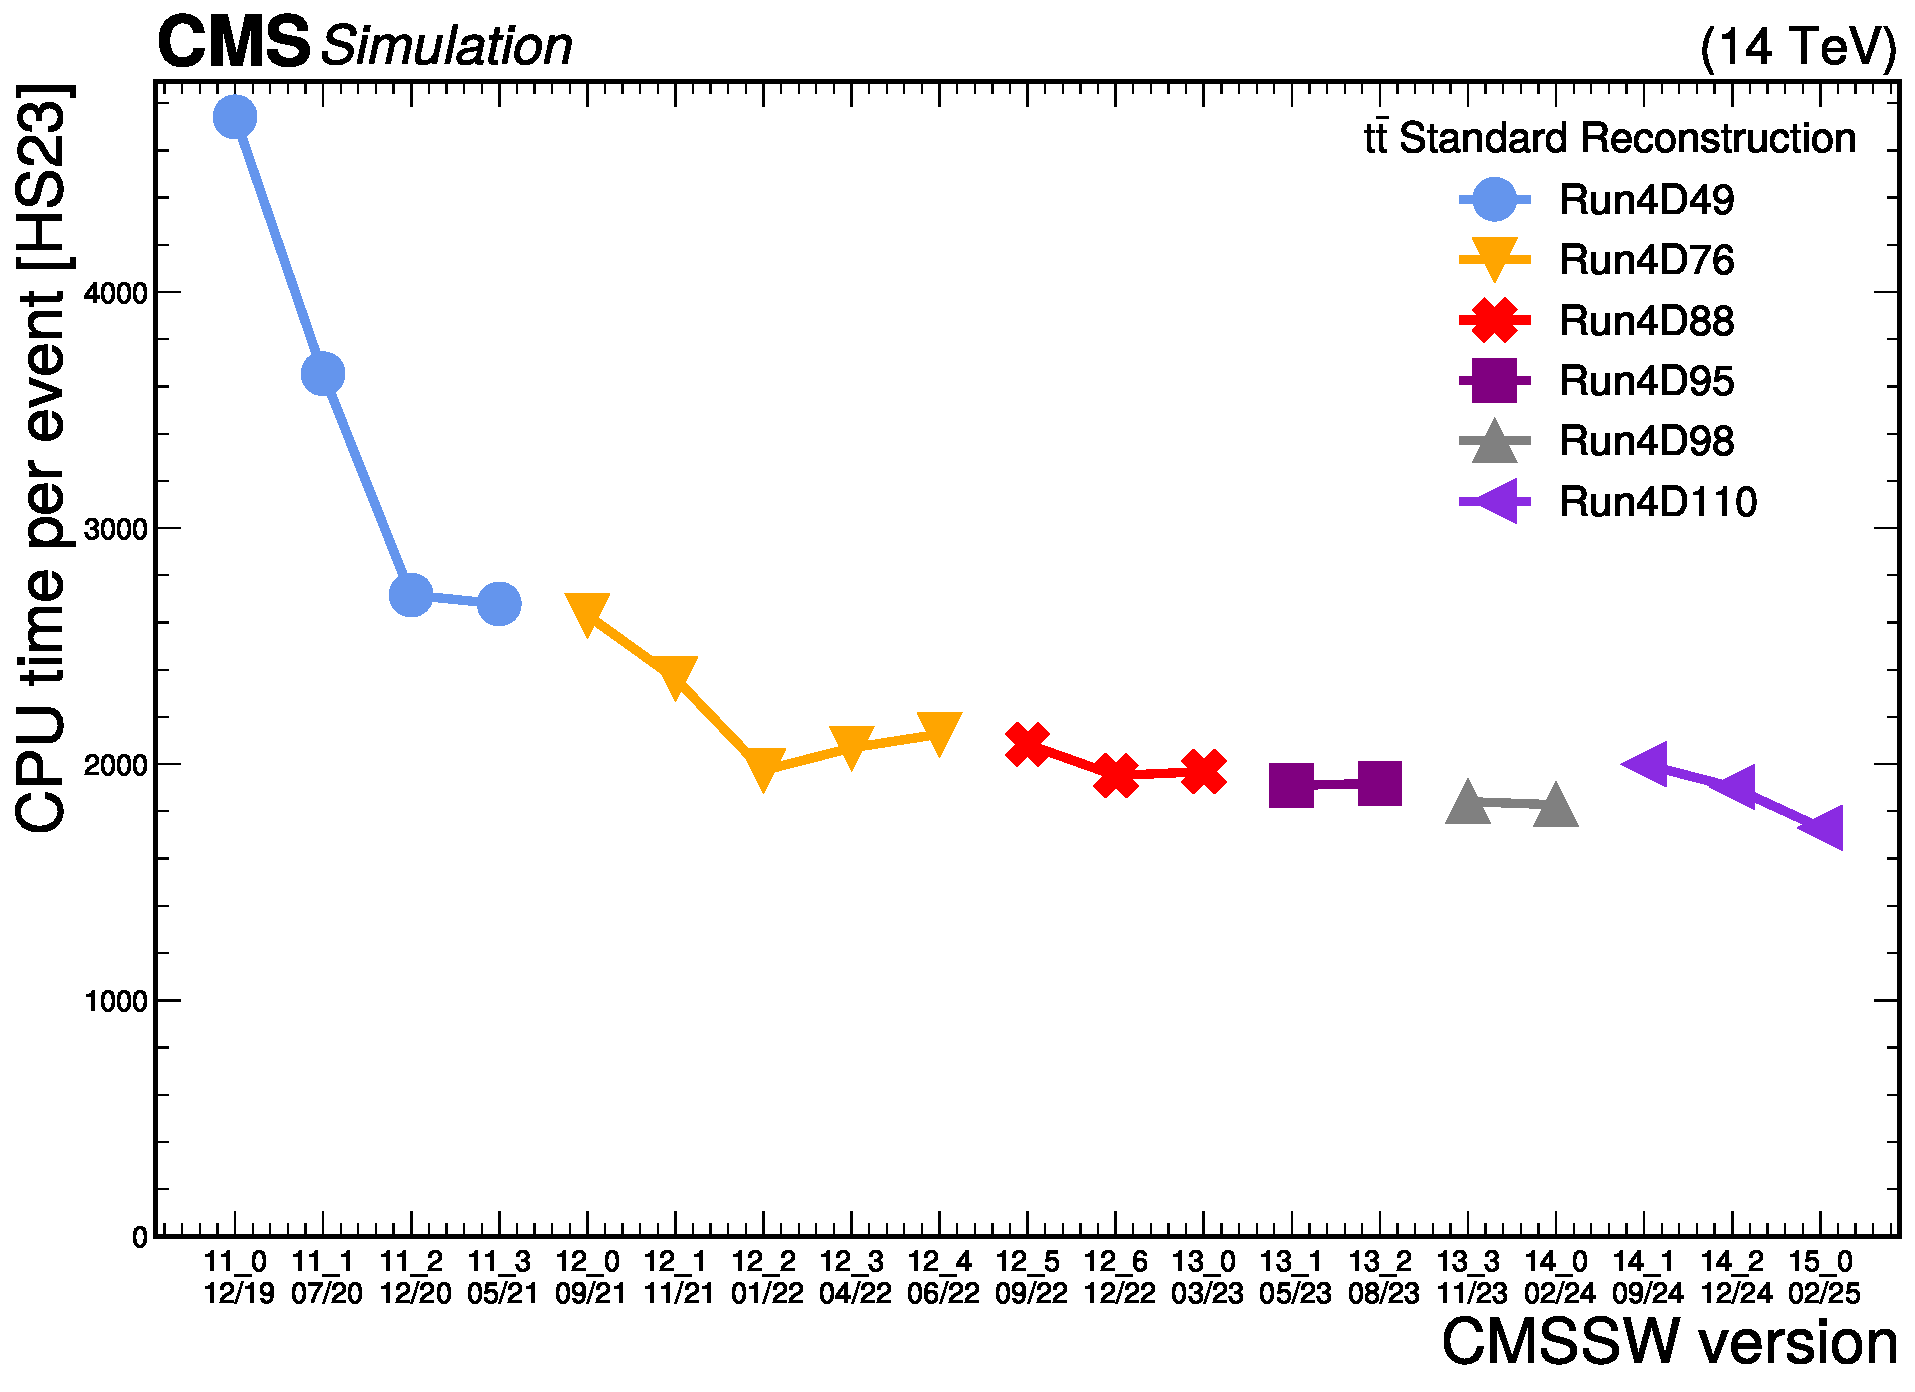
\includegraphics[width=0.95\textwidth]{figs/8 Reconstruction/major_release_timingCDR_colors (1).pdf}
    \caption{Absolute and relative reconstruction time per event for a \ttbar sample consumed by a \PhaseTwo CMS reconstruction workflow, as a function of the release version of the CMSSW software.}
    \label{fig:reco_major_release_timing}
\end{figure}

\begin{table}[tbhp]
    \footnotesize
    \centering
    \caption{\gls{CPU} time for \PhaseTwo reconstruction using the \gls{CMSSW}\_14\_0\_10 version from Feb. 2024. The time is measured for each reconstruction software package.
    The \gls{CPU} time assigned to the tracking package has been doubled to conservatively account for the computational cost of reconstructing displaced vertices. The Calorimeter package does not include the \gls{HGCAL}, which is run separately.}
    \begin{tabular}{|c|c|c|c|c|c|c|c|c|c|c|}
    \hline
    \rowcolor{tableheader} 
    & \multicolumn{5}{c}{Timing Fraction (\%)} & \multicolumn{5}{c}{Time (HS23-s)} 
    \\ \hline
    \rowcolor{tableheader}     
    Module                 &   PU100 & PU140 & PU150 & PU180 & PU200 & PU100 & PU140  & PU150    & PU180    & PU200    \\ \hline
    \cellcolor{tablerowheader}
    Tracking               &   42.2  & 50.4  & 52.2  & 55.5  &  56.9 & 244.1 &  481.1 & 566.5    & 822.8    & 993.6    \\ \cellcolor{tablerowheader}
    Pflow                  &   5.2   & 5.8   & 5.9   & 6.1   &  6.2  & 30.2  &  55.0  & 63.7     & 89.9     & 107.3    \\ \cellcolor{tablerowheader}
    Vertexing              &   6.0   & 5.9   & 5.8   & 5.7   &  5.7  & 34.6  &  56.4  & 63.4     & 84.5     & 98.6     \\ \cellcolor{tablerowheader}
    Muon                   &   4.4   & 4.6   & 4.5   & 4.2   &  4.1  & 25.7  &  43.5  & 48.4     & 62.8     & 72.4     \\ \cellcolor{tablerowheader}
    Elec./Phot.            &   4.9   & 4.3   & 4.3   & 4.2   &  4.1  & 28.3  &  41.4  & 46.6     & 62.1     & 72.4     \\ \cellcolor{tablerowheader}
    \gls{HGCAL}            &   3.8   & 3.2   & 3.0   & 2.7   &  2.6  & 22.2  &  30.7  & 33.1     & 40.2     & 44.9     \\ \cellcolor{tablerowheader}
    Jets                   &   2.7   & 2.5   & 2.4   & 2.3   &  2.2  & 15.4  &  23.6  & 26.1     & 33.6     & 38.7     \\ \cellcolor{tablerowheader}
    \gls{MTD}              &   3.0   & 2.6   & 2.5   & 2.3   &  2.2  & 17.1  &  25.0  & 27.3     & 34.1     & 38.7     \\ \cellcolor{tablerowheader}
    Tau                    &   1.8   & 1.7   & 1.7   & 1.7   &  1.6  & 10.3  &  16.4  & 18.5     & 24.6     & 28.7     \\ \cellcolor{tablerowheader}
    Calorimeter            &   0.9   & 0.5   & 0.5   & 0.5   &  0.5  & 5.2   &  5.0   & 5.6      & 7.5      & 8.7      \\ \cellcolor{tablerowheader}
    I/O                    &   17.0  & 14.1  & 13.3  & 11.7  & 11.0  & 98.3  & 134.9  & 144.5    & 173.1    & 192.2    \\ \cellcolor{tablerowheader}
    Misc                   &   8.2   & 4.3   & 3.9   & 3.1   &  2.8  & 47.5  &  41.4  & 42.6     & 46.3     & 48.7     \\ \cellcolor{tablerowheader}
    Total                  &   100.0 & 100.0 & 100.0 & 100.0 & 100.0 & 579.0 & 954.4  & 1\,086.1 & 1\,481.5 & 1\,745.0 \\ \hline
    \end{tabular}           
    \label{tab:recoTiming}
\end{table}

\subsection{R\&D to improve computing performance}

R\&D activities target improvements in the \gls{CPU} time performance and adaptation of reconstruction algorithms to run on \glspl{GPU}. Most of the effort is focused on reconstruction in new detectors, such as the \gls{MTD} and the \gls{HGCAL}, or on computationally intensive algorithms developed for precise reconstruction of vertices and trajectories in the tracker system and of particle showers in the calorimeters.

\subsubsection{Charged-particle tracking and vertexing}

The processing of charged particles in the tracker detector into particle trajectories is the most time-consuming component of the CMS reconstruction.  The association of hits to a given charged-particle trajectory becomes more complex with increasing pileup.  
The \PhaseTwo CMS tracker~\cite{CMS:2017TrackTDR} will cope with the high pileup and harsh radiation environment through an increased forward acceptance, improved radiation hardness, higher granularity, added capabilities to handle higher data rates, and a longer trigger latency than in \PhaseOne. The upgraded tracker device consists of an inner tracker, based on silicon pixel modules, and an outer tracker, made of silicon modules with strip and macro-pixel sensors.   

In the current scheme, the iterative tracking algorithm associates sets of hits, e.g., charged-particle energy deposits,  to form ``seeds'' from which an initial charged-particle trajectory is determined. This association, or pixel seeding, is performed using a \gls{CA} algorithm, which accounts for 10\% of the total reconstruction time. The \gls{CA} algorithm presently runs on \glspl{GPU}~\cite{Bocci:2020pmi} at the \gls{HLT}, while, for offline reconstruction, tuning the pixel seeding parameters and evaluating the physics performance achieved with this algorithm are ongoing work. The \textbf{Reco.3} activity in Table~\ref{tab:reco-improvements} is expected to deliver a \gls{CA} algorithm that runs 60\% faster on \glspl{CPU}, yielding an 8\% time performance improvement in the total reconstruction time. 

Although the algorithm is designed to run on \glspl{GPU}, there is a potential risk of a reduced fraction of \gls{CPU} time offloaded to \glspl{GPU}. The reason is that the algorithm runs over a collection of input data stored in a \gls{SoA} that needs to be transferred from a \gls{CPU} to a \gls{GPU}. As the pileup increases, the size of this \gls{SoA} may become too large for storage on the \gls{GPU}. Once the porting and optimization for offline use are completed, the goal is to offload up to 90\% of the \gls{CPU} workload to the \gls{GPU}. This 90\% offload figure accounts for any potential data transfers or conversions to the \gls{SoA} format. 

This applies to all algorithms currently being offloaded to the \gls{GPU}, as well as those that will be in the future. There is still potential to improve this offload percentage further and achieve 100\% \gls{GPU} offload if the data structures are designed with the \gls{SoA} paradigm in mind. Additionally, if subsequent steps of the reconstruction process, which produce collections consumed by the next step, are also run on the \gls{GPU}, the \gls{SoA} will reside entirely on the \gls{GPU}, eliminating the need for data transfers.
Extending the \gls{CA} algorithm to the first layers of the \PhaseTwo outer tracker is currently under consideration.

The next track building step, based on the \gls{CKF}~\cite{CMS:2014pgm}, propagates the seed trajectory through subsequent layers of the tracker.
The mkFit~\cite{Lantz:2020yqe} algorithm is a recent implementation of the \gls{CKF} that uses vectorized operations and a lightweight representation of the tracker geometry. In \RunThree, this algorithm has, so far, achieved a factor of~6 speed-up while retaining comparable physics performance~\cite{CMS-DP-2022-018}. The objective of the \textbf{Reco.4a} activity in Table~\ref{tab:reco-improvements} is to implement mkFit for track building and final fitting within \PhaseTwo reconstruction, where it should yield a similar speed-up factor, resulting in a 65\% total tracking time reduction and 7\% savings in total reconstruction time. 

Concurrently with this work, complementary track-finding algorithms amenable to parallelization are under design. The most advanced is the \gls{LST} algorithm, listed as \textbf{Reco.4b} in Table~\ref{tab:reco-improvements}, which takes advantage of the outer tracker ``\pt-modules'' design to reduce the combinatorics in the track building. The pairs of local hits detected in this configuration of two parallel sensors separated by a few millimeter gap are combined to form ``segments''.  Segments can then be combined with other segments or with inner tracker seeds to create progressively longer tracks. A standalone implementation of the \gls{LST} algorithm demonstrates that good performance, in terms of efficiency and misreconstruction rate, can be achieved while efficiently using multiple streams on \glspl{GPU}. 

The integration of the \gls{LST} algorithm in \gls{CMSSW} has already started; \gls{LST} can be run either as a standalone track finder or used to reduce the complexity of the pattern recognition as input to the \gls{CKF}. The impact of \gls{LST} on computing performance depends on how it is combined with mkFit. In parallel with the above-mentioned algorithm development work, ML replacements for track building based on \glspl{GNN} are under study to achieve better physics accuracy while preserving or improving \gls{GPU} offload capabilities.

Two conditions must be satisfied to use \gls{GPU}-enabled algorithms in the track-building step. The first requires that 50\% of the track building is done by the \gls{LST}, while the remaining 50\% is done using mkfit; the second requires that 100\% of the track building currently performed by \gls{CPU}-based mkfit is carried out by the \gls{LST} or a yet-to-be-developed \gls{GPU} based algorithm. These two assumptions will enter the medium and low-probability compound R\&D scenarios, respectively, summarized in Table~\ref{tab:effects-of-rnd-scenarios-gpu}.

It should be noted that reconstruction of highly displaced tracks has not yet been implemented in the context of the \PhaseTwo.  As a ``placeholder'' value, and until an accurate estimate becomes possible, displaced tracks double the ``Tracking'' time component, as reflected in Table~\ref{tab:recoTiming}. Developments such as \gls{LST} may, however, significantly improve this projection. 

Additionally, several components of the tracking chain have not yet had their potential for \gls{GPU} offloading fully explored. This remains an active area of R\&D that could result in further optimizations, potentially reducing the total \gls{CPU} time by an additional 5\%. This assumption is incorporated in \textbf{Reco.9a} of Table~\ref{tab:reco-improvements} and will enter the low-probability compound R\&D scenario summarized in Table~\ref{tab:effects-of-rnd-scenarios-gpu}.

The reconstruction of electrons is also being upgraded to take advantage of \glspl{GPU}. The goal of the \textbf{ Reco.6} activity in Table~\ref{tab:reco-improvements} is to achieve a reduction in the number of tracker seeds used in the electron track reconstruction, which currently takes approximately 50--70\% of the overall electron reconstruction time. It will also leverage the track seed collection already generated by the \gls{CA} algorithm and available on the \gls{GPU}. This reduced collection is then propagated to the electron track reconstruction algorithm, the \gls{GSF} tracking, which takes up the majority of the remaining electron reconstruction time. 

Finally, the reconstruction of primary collision vertices has also been re-engineered to profit from \glspl{GPU} (\textbf{Reco.2} activity in Table~\ref{tab:reco-improvements}). The track clustering is performed regionally, in blocks of tracks, which are subsequently merged. The vertex position fit has been replaced by a weighted mean algorithm that uses the track impact-parameter error as a weight.  The vectorized vertexing algorithm achieves an 80\% reduction in time per event consumption when run on \glspl{CPU} (6\% in the total reconstruction time), while delivering comparable physics performance. 
It is predicted that, once performance portability work is completed and the code is optimized and validated, the offload of the algorithm to \gls{GPU} would result in a potential throughput increase of a factor of~10. 

In \PhaseTwo, a novel \gls{MIP} Timing Detector will provide a time measurement for charged tracks in front of the calorimeters with a $\pm$30--40\unit{ps} uncertainty at startup, degrading to $\pm$50--60\unit{ps} by the end of the detector's life. 
Although its algorithms are not large consumers of \gls{CPU} resources, only 3\% of the total reconstruction time per event (see Table~\ref{tab:recoTiming}), it is worth describing them in some detail because the \gls{MTD} is a new detector type within the \PhaseTwo configuration. 

Charged particle tracks, reconstructed in the silicon tracker, are linked to the clusters measured by the \gls{MTD} layers, and the corresponding measured times are back-extrapolated to the point of closest approach to the beam line. This extrapolation is clearly dependent on the mass assigned to the track, since only its momentum is reconstructed. The \gls{MTD} apparatus behaves as a time-of-flight detector once tracks are clustered into primary vertices, exploiting the constraint of equal time at the vertex within uncertainties for all tracks associated with it.

The determination of the optimal mass hypothesis is made at the time of vertex reconstruction, requiring the best possible compatibility of back-extrapolated times within their uncertainties. In this way, the vertex time reconstruction and track particle identification become intimately connected. 

An iterative procedure is used for a 4D vertex reconstruction, i.e., a fit of vertices using both the space and time measurements simultaneously: a time for vertices is computed from tracks clustered using the standard 3D vertex reconstruction based on pure spatial information, and this is used for an initial assignment of the mass hypothesis to each charged track associated with the vertex. Then, the vertex reconstruction is repeated by exploiting also the time information and the corresponding estimated uncertainty in the track clustering. The optimal mass hypothesis is again determined from this final output. Further improvements to this strategy are actively pursued, also to make the procedure computationally more efficient, which could be of interest for the stringent speed requirements of \gls{HLT} reconstruction.

The computationally most intensive part of the track timing reconstruction is the cluster-track matching and time extrapolation algorithm, which currently consumes 2\% of the total \gls{CPU} reconstruction time.
Although the offloading of the \gls{MTD} algorithm to \glspl{GPU} has not yet been explored, it remains an active area of R\&D that may enable the full offloading of the \gls{MTD} reconstruction algorithm, potentially reducing the total \gls{CPU} time by an additional 3\%. 

In parallel, ML algorithms based on GravNet, a type of \gls{GNN} with an object condensation loss function, are under study to improve the physics performance of the 4D vertex algorithm while producing code amenable to \gls{GPU}.
These options are incorporated in \textbf{Reco.9b} of Table~\ref{tab:reco-improvements} and will enter the low-probability compound R\&D scenario summarized in Table~\ref{tab:effects-of-rnd-scenarios-gpu}.


\subsubsection{Calorimeter clustering and linking}

The CMS endcap calorimeters will be completely replaced by the \gls{HGCAL} in \PhaseTwo. This upgrade will allow CMS to study particle showers and boosted objects in much more detail, while coping with the harsh radiation environment and the high levels of pileup at the \gls{HL-LHC}. Processing the large number of individual signals in this highly segmented apparatus will, however, be computationally expensive.

The \gls{HGCAL} reconstruction is currently based on \gls{TICL} approach, which uses the time, position, and energy of each detector channel to reconstruct final-state physics particles, assigning them a particle type probability and calculating their kinematics.
\gls{TICL} has been designed to run on heterogeneous platforms, with data structures optimized for \glspl{GPU}.
A first version of the \gls{HGCAL} \gls{TICL} full reconstruction takes about 2\% of total \PhaseTwo reconstruction time on a traditional single \gls{CPU} core using a sample with 200 pileup interactions. 

While the \gls{CPU} execution time is not expected to be reduced significantly before \RunFour, the layer-level energy clustering (CLUE) and the 3D pattern recognition (CLUE3D) algorithms represent approximately 90\% of the \gls{CPU} time and are highly parallelizable, with early prototypes achieving an event throughput increase of a factor of~10--15 when offloaded to \glspl{GPU}. This is the focus of the  \textbf{Reco.5a} activity in Table~\ref{tab:reco-improvements}, with a goal to maintain this computing performance, while improving physics precision. The extension of the \gls{TICL} framework to the barrel calorimeters is the goal of the \textbf{Reco.5b} activity in Table~\ref{tab:reco-improvements}. 

Multiple complementary ML-based R\&D lines are being actively studied to scale up ML use in \gls{HGCAL} reconstruction, including GNN-based linking, transformer-based approaches, and MLPF-inspired techniques within the \gls{TICL} framework. These efforts aim to improve specific reconstruction stages while preserving the modularity, robustness, and transparency of the overall reconstruction. The ML efforts are generically represented as \textbf{Reco.8} in Table~\ref{tab:reco-improvements}. Depending on the solution implemented, up to 90\% of the \gls{HGCAL} reconstruction code would be offloaded to \glspl{GPU}.

Once the basic detector-level objects have been reconstructed, CMS relies on a particle-flow algorithm to combine information from the various subdetectors~\cite{CMS:2017yfk} into an optimal event reconstruction based on individual particles. The current rules-based implementation of this algorithm consumes about  10\% of the reconstruction time. \textbf{Reco.7} in Table~\ref{tab:reco-improvements}~\cite{Pata:2021oez}, is an approach based on a transformer architecture (\gls{GNN}) that could result in offloading up to 90\% of the particle-flow code to \glspl{GPU}, for a potential speed-up of up to an order of magnitude.

In addition to the previously discussed algorithms, there are other components of the reconstruction process that have not yet been fully explored in terms of \gls{GPU} offloading but present promising opportunities for future R\&D. This includes muon reconstruction, which currently consumes up to 5\% of the total \gls{CPU} time. Additionally, smaller algorithms used for the reconstruction of higher-level objects, such as jets and taus, which often rely on machine learning techniques, contribute another 10\% of the total \gls{CPU} time. 

Ongoing developments may enable the offloading of the muon reconstruction, potentially reducing \gls{CPU} time by up to 5\%. Furthermore, partial offloading of some of these smaller algorithms could lead to an additional reduction in \gls{CPU} time of approximately 2\%. These assumptions are incorporated respectively in \textbf{Reco.9c} and \textbf{Reco.9d} of Table~\ref{tab:reco-improvements} and will enter the low-probability compound R\&D scenario summarized in Table~\ref{tab:effects-of-rnd-scenarios-gpu}.

\subsection{Data format size reduction}
\label{sec:rawprime}

A novel compression algorithm was used in 2023 for all hadronic events in heavy-ion collisions, including the minimum-bias \gls{RAW} data samples. By reducing the information stored per silicon-strip cluster and applying stronger lossless \textsc{ROOT} compression, CMS saved a factor of~2 in the \gls{RAW} data size per event, enabling the collection of a larger minimum-bias event sample while staying within network limitations from P5. Called the \gls{RAW}$^\prime$ data format, this could potentially be used for certain PDs in proton-proton collisions (see Table 11, Row 1 in~\cite{Software:2815292}).

In \RunThree, the total compression factor achieved for proton-proton events when performing online reduction and applying lossless algorithms (offline) to a full \gls{RAW} data file is approximately 60\%. The plan for \PhaseTwo, however, is to perform some of the data reduction at the hardware level. 

While the inner tracker read-out chip will use a form of binary tree encoding to reduce the \gls{RAW} data size (see Section~6, Fig. 47 in Ref.~\cite{ITcomp}), the outer tracker will be read out in digital form and rely on a \gls{RAW}$^\prime$ data reduction strategy at the hardware level. In both cases, lossless compression algorithms should perform less efficiently. Conversely, only the fast \gls{HGCAL} readout used at the \gls{L1T} level includes data compression, while data at the \gls{DAQ} and \gls{HLT} level is not further reduced.

Conservatively, based on an event size comparison after online and offline compression in \RunThree, the \gls{RAW} event sizes presented in Table~\ref{tab:event-sizes} could be reduced by approximately 15\%.

The \textbf{DataF.1} research line aims to verify the 15\% offline compression reduction already achieved in \RunThree and explore how to further reduce the \gls{RAW} data size to a total target of 30\%. For example, although the \gls{RAW}$^\prime$ technique at the hardware level is not applicable to the \gls{HGCAL} (ASIC cannot be further modified), data reduction may be achieved by raising hit thresholds, or applying filters after local reconstruction in the HLT. More efficient offline algorithms can also be used across all subdetectors, albeit at the expense of \gls{CPU}. 

Simultaneously, the \textbf{DataF.2} activity will target size reductions on the order of 15\% for derived data formats (\gls{AOD}, miniAOD, and NanoAOD) using more effective data compression algorithms, as well as core software improvements that include removal of dynamic polymorphism from data types, integration of an RNTuple-based source and output module into \gls{CMSSW}, and migration to a columnar data format by subdetector at the preprocessing level.
A \textbf{DataF.3} activity will focus on reducing AODSIM production by 50\%, limiting the data sets to background and selected signal samples, and saving tape and disk resources.

\subsection{Detector alignment, calibration, and synchronization}
\label{sec:pcl}

\subsubsection{The prompt calibration loop in \RunThree}

The \gls{PCL} is an automated procedure for deriving new calibration and alignment constants while collecting LHC data, in order to make them available for prompt reconstruction. It takes as input the data from the express stream, which is typically reconstructed within seven to eight hours, and uses it for the various calibration and alignment workflows. 

Once the new calibration constants are derived and validated, they are automatically uploaded to the conditions database for use in event reconstruction. In order to allow for sufficient time to derive and validate these constants, the prompt reconstruction at \TierZero is delayed by 48 hours.

There are currently about 15 workflows that entail aligning the tracker, measuring the beamspot position, measuring response corrections for the \gls{ECAL}, and performing additional measurements, such as gains and pedestals, for a number of subsystems.

A general \gls{PCL} workflow consists of a series of consecutive, chained steps. First, an AlcaReco data set is created from express data. Then an AlCaSkimming is run on the AlCaReco, producing an AlCaPrompt output that includes histograms for deriving conditions. An AlCaHarvesting step produces, from the AlCaPrompt, a local database containing the resulting calibrations or alignment constants, along with their intervals of validity (IOVs). Finally, a daemon monitors the output of the AlCaHarvesting step and, in the central database used for prompt reconstruction, deploys the conditions from the local database.

For workflows that require more than 48 hours to execute, a Jenkins-based automated framework was developed during \LSTwo and deployed for \RunThree. It takes the promptly reconstructed data sets as input and uses the accumulated data to derive the alignment and calibration constants that require a sizable sample. Typical workflows use a few inverse femtobarns of data to derive the conditions for future (prompt) reconstructions.

\subsubsection{The prompt calibration loop for \PhaseTwo}

The fundamentals of the \RunThree workflows are expected to remain unchanged for \PhaseTwo operations. Although the number of detector channels will increase, the algorithms for aligning and calibrating the current detectors are anticipated to scale effectively with \PhaseTwo computing resources.

One of the most resource-intensive workflows is tracker alignment. The number of free parameters to determine during the alignment process is not expected to increase significantly in complexity in \PhaseTwo, because while the total number of sensors in the inner and outer trackers will be larger, the overall number of modules to be aligned will be similar to that in \PhaseOne. A source of uncertainty, however, comes from the tilted modules in the outer tracker, which may demand a more complex procedure to avoid misalignment in weak modes leading to significant tracking errors.


The number of channels in the calorimeters will increase substantially due to the higher granularity of forward calorimetry. However, feasibility studies for the \gls{HGCAL} calibration, which is performed with minimum-ionizing particles, have already been successful, and the calibration is expected to remain manageable within \PhaseTwo resources.

A new aspect will be the synchronization workflows, introduced to monitor and correct time alignment, clock phase shifts, readout delays, and detector latency mismatches. Currently limited to a few subsystems, but in \PhaseTwo will be expanded to cover most of CMS and reach a new level of precision. The complexity of these algorithms is low, and the resources required to process them will not pose any issues.

\subsubsection{Payload handling}

In the context of applying the conditions to data, the key metrics are the size of each condition payload and the duration of the IOVs for each condition. These factors determine the size of the database hosting the conditions, the data flow required to access them, and the memory footprint of the jobs that apply them.

In \PhaseTwo, the number of CMS channels requiring some form of correction, be it calibration or synchronization, will be of the order of 30 million. The size of a typical payload is expected to be of the order of a few hundreds megabytes.

While the alignment and energy calibration are not expected to evolve on a timescale particularly different from \PhaseOne, despite the increased radiation, synchronization may require frequent delivery of corrections. From preliminary tests of the first prototypes for the upgraded electronics, it seems reasonable to assume that this frequency will not exceed that of the reconfiguration of the boards, which is expected to happen at most once per run, that is, once every $\mathcal{O}(\text{1 hour})$.

The amount of condition data to hold in a database corresponds then to some 100\unit{MB/hour}, which seems a reasonable number to handle with today’s technologies and will not constitute a challenge for \PhaseTwo computing resources.

A number of tests are planned to confirm these estimates based on more accurate simulations. This will take place within dedicated \gls{CSA} exercises, which will provide additional insights for the main supporting infrastructures for the \gls{PCL}. These include the \TierZero, responsible for the reconstruction of express and physics streams, the production of AlCaRecos, AlCaPrompt, and the upload of the conditions to the condition database; the condition database itself, Oracle-based; the Frontier middle tier, which stores the results of the database queries in a hierarchical set of Squid proxies, to provide an efficient load-balanced caching system.

\subsection{Summary of reconstruction-related and data formats R\&D activities} 

Table~\ref{tab:reco-improvements} lists the various R\&D activities discussed in this section related to reconstruction and data formats, with estimates of the potential impacts and our estimation of the probability of success or adoption on the timescale of the beginning of \RunFour. 
%In our previous documentation on planning for offline software and computing for Phase 2~\cite{Software:2815292} published in 2022, 
%Table 7, Row 1 corresponds to Reco.1, 
%Table 7, Row 2 no status,
%Table 7, Row 3 corresponds to Reco.4a, 
%Table 7, Row 4 was achieved,
%Table 9, Row 2 corresponds to Reco.3,
%Table 9, Row 3 no status,
%Table 9, Row 4 corresponds to Reco.6,
%Table 9, Row 5 corresponds to Reco.5,
%Table 9, Row 6 corresponds to Reco.8, and
%Table 9, Row 7 corresponds to Reco.7,
% and Reco.2 and Reco.4b are new.


% Edited by Charis 25.2.2025
\begin{table}[tbph]
    \centering
    \caption{Summary of reconstruction-related R\&D activities with estimated impacts and probabilities of success on the timescale of the beginning of \RunFour. The impact of the \textbf{DataF} activities marked with an (*) include the contributions from \textbf{CoreSoft.1}, \textbf{CoreSoft.6} and \textbf{CoreSoft.7} displayed in Table~\ref{tab:fwk-improvements}. \gls{CPU} time savings or offloaded to \glspl{GPU} is expressed as a fraction of the total \gls{RECO} time.}
    \begin{tabular}{|c|c|c|c|}
    \hline
    \rowcolor{tableheader} 
              &                                  &                                                   & Probability      \\ 
    \rowcolor{tableheader}
              & Description                      &       Impact                                      & of Success       \\ 
    \rowcolor{tableheader}
              &                                  &   (Fraction of total RECO CPU time)   & and/or Adoption  \\ \hline
    \cellcolor{tablerowheader}
              & Continuous Code                  & 5\% CPU speed-up                             &                  \\
    \cellcolor{tablerowheader}
    Reco.1    & Optimization                     & (per year for avg. evt.)                          & Success: High    \\ \hline
    \cellcolor{tablerowheader}
              & Vertex algorithms:               & Takes 6\% of total time/evt.                      &                  \\
    \cellcolor{tablerowheader}
    Reco.2    & {code vectorization }            & 80\% {speed-up on CPU}                       & Adoption: High   \\
    \cellcolor{tablerowheader}
              & {GPU porting}              &     {($>$90\% of CPU time }                 &                  \\ 
    \cellcolor{tablerowheader}
              &                                  &  offloaded to GPU)                        &                  \\ \hline
    \cellcolor{tablerowheader}
              & Pixel-track seeding:             & Takes 12\% of total time/evt.                     &                  \\
    \cellcolor{tablerowheader}
    Reco.3    & GPU-targeted               & 60\% {speed-up on CPU}                       & Adoption: High   \\
    \cellcolor{tablerowheader}
              & algoritms                        &  {($>$90\% of CPU time }                    &                  \\ 
    \cellcolor{tablerowheader}
              &                                  &  offloaded to GPU)                        &                  \\ \hline
    \cellcolor{tablerowheader}
              &  Tracking: mkFit                 & Takes 10\% of total time/evt.                     & Success: High    \\
    \cellcolor{tablerowheader}
   Reco.4a    &  algorithm + ML                  & 65\% {speed-up on CPU}                       & Adoption: Medium \\ \hline
    \cellcolor{tablerowheader}
              &  {Tracking: mkFit/LST}     & {50\% mkFit CPU time done by LST}     & Success: High    \\
    \cellcolor{tablerowheader}
   Reco.4b    &  combination + ML                & {($>$90\% of LST offloaded to GPU}) & Adoption: High   \\ \hline
    \cellcolor{tablerowheader} 
              & {HGCAL: TICL}        & Takes 2\% of total time/evt.                      & {Success: High}  \\
    \cellcolor{tablerowheader}
    Reco.5a   & framework on GPU         & {($>$90\% time/evt. }                             & (focusing on     \\
    \cellcolor{tablerowheader}
              &                                  &  offloaded to GPU)                        & physics gains)   \\ \hline
    \cellcolor{tablerowheader} 
              & {Calorimeters: TICL}       & Takes 1.7\% of total time/evt.                    &                  \\
    \cellcolor{tablerowheader}
    {Reco.5b} & {for the barrels }               & {($>$90\% time of calorimeter}                    & {Success: High}  \\
    \cellcolor{tablerowheader}
              &       on GPU             &   {barrels offloaded to GPU})             &                  \\ \hline
    \cellcolor{tablerowheader}
              & Electrons: GPU-            & {Takes 3.5\% time/evt.}       &                  \\
    \cellcolor{tablerowheader}
    Reco.6    & targeted seeding                 & {($>$90\% time }                                  & Success: Medium \\
    \cellcolor{tablerowheader}
              & algorithms                       & offloaded to GPU)                         & Adoption: Medium \\ \hline
    \cellcolor{tablerowheader}
              & particle flow:                   &  {Takes 10\% total time/evt.}                     &                  \\
    \cellcolor{tablerowheader}
    Reco.7    & GPU-targeted recon-        &    {($>$90\% time }                               & Success: Medium  \\
    \cellcolor{tablerowheader}
              & struction with ML          &   offloaded to GPU)                       &                  \\ \hline
    \cellcolor{tablerowheader}
              &  HGCAL: ML           &  Takes 3\% of total time/evt.                     &                  \\
    \cellcolor{tablerowheader}
    Reco.8    &  reconstruction                  &  {($>$90\% time }                                 &  Success: Medium \\
    \cellcolor{tablerowheader}
              &                                  &    offloaded to GPU)                      &                  \\ \hline
    \cellcolor{tablerowheader}
              &  Tracking: Only LST        & Takes 15\% of total time/evt    &               \\ 
    \cellcolor{tablerowheader}
    Reco.9a   &  and other GPU-based       &  plus an additional 5\%                           &  Success: Low    \\
    \cellcolor{tablerowheader}    
              & algorithms                       &  for other tracking steps                         &                  \\\hline
    \cellcolor{tablerowheader}    
    Reco.9b   & MTD: GPU-based + ML &  Takes 3\% of total time/evt                      & Success: Low     \\\hline
    \cellcolor{tablerowheader}
    Reco.9c   & Muon: GPU-based            & Takes 5\% of total time/evt                       & Success: Low     \\\hline
    \cellcolor{tablerowheader}
              & Other: GPU-based           & Up to 2\% of total time/evt comb-                 &                  \\  
    \cellcolor{tablerowheader}
    Reco.9d   & algorithms                       & ing several small (in terms of                    & Success: Low     \\ 
    \cellcolor{tablerowheader}
              &       &  CPU time) offloaded to GPU           &                  \\ \hline
    \cellcolor{tablerowheader}
              &                                  &  Reduction with respect                           &                  \\
    \cellcolor{tablerowheader}
    DataF.1   &  RAW event size            &  to Table~\ref{tab:event-sizes}  by 30\%$^*$      & Success: Medium  \\  \hline
    \cellcolor{tablerowheader}
        \cellcolor{tablerowheader}
              &  Derived data                    &  Reduction with respect                           &                  \\
    \cellcolor{tablerowheader}
    DataF.2   &  event size                      &  to Table~\ref{tab:event-sizes} by 15\%$^*$       & Success: High    \\ \hline
    \cellcolor{tablerowheader}
    DataF.3   &  AOD data set               &  reduction by 50\%                                & Success: High    \\ \hline

    \end{tabular}
    \label{tab:reco-improvements}
\end{table}

\clearpage

%%%%%%%%%%%%%%%%%%%%%%%%%%%%%%%%%%%%%%%%%%%%%%%%%%%%%%%%%%%%%%%%%%%%%%%%%%%%%%%%
%
% WORKFLOW MANAGEMENT
%
%%%%%%%%%%%%%%%%%%%%%%%%%%%%%%%%%%%%%%%%%%%%%%%%%%%%%%%%%%%%%%%%%%%%%%%%%%%%%%%%
% \clearpage
% \input{tex/08_workflow_management.tex}
\section{Workflow management}
\label{sec:Workflow}

A \gls{WM} system for a \gls{HEP} experiment, such as CMS, consists of a set of central services and a pool of distributed agents that execute computing workflows built to satisfy requests for different types of data sets utilized in data analysis. The central services perform actions such as workflow management and monitoring, workflow decomposition into work elements, and automatic placement of input and output data. The \gls{SI} completes the system, providing resources for all CMS computing tasks.

CMS has concluded a review of its \gls{WM} system to re-examine its long-term sustainability and challenges, including collaborative, for the lifetime of the \gls{HL-LHC} program. Motivations are internal effort shortfalls within the current system and external forces requiring significant change, such as the full adoption of heterogeneous resources. The next sections describe the current \gls{WM} system and its possible evolution to address the challenges. 

During \RunThree, LHCb, ATLAS, and ALICE all have their own \gls{WM} systems. However, LHCb and ATLAS also share their solution with non-LHC experiments and therefore have some multi-virtual-organization capabilities. CMS's submission infrastructure is common to many experiments and the Open Science Grid. Although Rucio serves as the backbone of CMS data management and is shared with ATLAS and other non-LHC experiments, the workflow management system remains experiment-specific. Given that many technological challenges are common across all LHC experiments, it is important to consider even revolutionary approaches to \gls{WM} that consolidates the systems of all LHC experiments.

\subsection{The current workflow management and system integration}

\label{sec:wm_sys_integration}
The role of the CMS \RunThree \gls{WM} and \gls{SI} systems, shown schematically in Fig.~\ref{fig:prod_chain} and described in Ref.~~\cite{wm_description}, is to efficiently manage prioritized requests and orchestrate storage and compute resources in order to deliver the requested data sets to the collaboration. 

\begin{figure}[htbp]
    \centering
    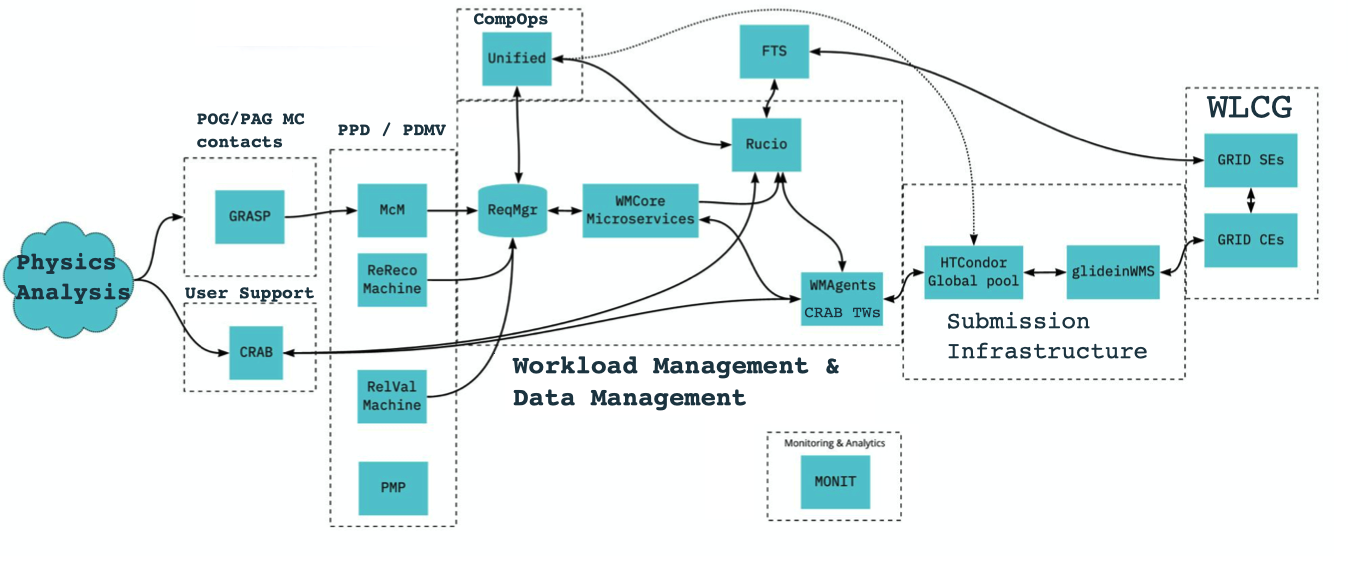
\includegraphics[width=\textwidth]{figs/workflow_management/production_chain_and_WM.png}
    \caption{CMS production chain, including the \gls{WM} and \gls{SI} systems described in the main text.}
    \label{fig:prod_chain}
\end{figure}

The pool of agents, called WMAgents, acquires and processes fragments of the workflow, materializing them into compute jobs and performing all tasks related to data dependencies and bookkeeping. The \gls{SI}, described in Ref.~\cite{SI_description}, consists of a number of federated HTCondor~\cite{htcondor} pools, aggregating resources mainly from the \gls{WLCG}, as well as increasingly from high-performance computing and cloud providers. Compute jobs, commonly referred to as payload jobs, are submitted by the WMAgents to the \gls{SI} HTCondor scheduler agents' execution point queues. 
Resource provisioning in the \gls{SI} is performed by the GlideinWMS components~\cite{ISfiligoi_2008,glidein_wms}. Pilot jobs, acting as resource requests, are submitted to the resource providers \glspl{CE}, which are compatible with payload jobs' requirements. Once acquired, these resources join the HTCondor pools as dynamically partitionable slots, which are subsequently matched to suitable payload jobs according to their resource requests and priorities.  

The CMS \gls{WM} system supports two main workflow configuration modes: StepChain and TaskChain. In StepChain workflows, multiple processing steps are executed sequentially as part of a single payload job. This mode is mainly used when multiple steps (e.g., digitization and reconstruction) can be handled within a single job, reducing overhead by avoiding the need to create separate payload jobs and manage intermediate output files. A StepChain workflow, therefore, might include all \gls{MC} simulation steps (\gls{GEN}-\gls{SIM}-\gls{DIGI}-\gls{RECO}-\gls{AOD}-MINI/NanoAOD) in a single batch job.

In the case of TaskChain Workflows, separate payload jobs are created for each step in multi-task processing. Compared to StepChain, this is a more flexible yet complex workflow model with increased overhead, as it allows \gls{WM} to apply different configurations (e.g., compute resource requirements such as memory) to each task in the chain, as well as to define complex dependencies between steps. TaskChain workflows also allow executing tasks that require different environments at each step.

\subsection{Interplay between workflow and data management systems}

In managing central production workflows, the CMS \gls{WM} system reads and produces hundreds of Terabytes every day. In order to efficiently supervise operations such as data set transfers, replication, deletion, and data locality, the CMS experiment relies on a \gls{DM} system (Sec.~\ref{sec:data-management}) built on Rucio. The \gls{WM} system therefore interfaces with the \gls{DM} in a number of ways, namely
\begin{itemize}
    \item verifying the current location for a given data set,
    \item requesting the data transfer and replication to disk and/or tape endpoints,
    \item creating identifiers for data sets under production,
    \item securing data to avoid data loss.
\end{itemize}

A strong and efficient interplay between \gls{DM} and \gls{WM} is critical for efficiently using compute resources, maximizing event throughput, and delivering useful data to the collaboration. 

From the diverse levels of data granularity supported by Rucio, \gls{WM} relies on three: container, data set and file replica. These three layers are compatible with the data hierarchy used in CMS and supported by the \gls{DBS}~\cite{Afaq_2008}. To maintain a manageable data system, the \gls{WM} typically handles the container and data set levels, leaving the lower file-replica level to the actual \gls{DM} system. 

In addition to Rucio, \gls{DBS} is another critical component of the CMS \gls{DM} system, dealing with metadata. The \gls{DBS} helps the collaboration understand the data composition, how it was produced, the workflow configuration, and the \gls{CMSSW} releases used. Data is structured into the data set, block, and file layers, which are directly equivalent to the Rucio container, data set, and file replica. Additionally, \gls{DBS} stores the actual content type of each file, tracking metadata even deeper than the file level, including run number, luminosity block, and event count.

Another hybrid tool commonly used by CMS \gls{WM} for data lookup is called the \gls{DAS}~\cite{KUZNETSOV_2010}, which has the capability of interfacing with many different \gls{WM} and \gls{DM} web-services, such as \gls{DBS}, Rucio, and a request manager. Note, however, that given its nature of data aggregation, \gls{DAS} does not own any data itself. Instead, \gls{DAS} fetches metadata from the actual web services, enriching it with aggregation and caching. 

\subsection{Results of the 2025 workflow management review}

The committee that reviewed the current workflow management system found that, as functional and scale requirements have grown, workflow management has evolved reactively, driven by operational needs rather than a coordinated, sustainable plan. The committee determined that CMS does not currently have a workflow management system suitable for \RunFour and beyond. The existing system, as assessed by its experts, is unsustainable and not evolvable. A viable path forward requires CMS to commit and sustain a multi-year effort to build or integrate a new system. The committee makes the following recommendations, laid out in three phases (steps) described below. 

Requirements and planning (step 1):

\begin{itemize}
    \item CMS should formally define the requirements for a future workflow management system, addressing both traditional HTC workflows and the potential need for tightly coupled computations.
    
    \item The experiment should also identify the elements needed to support user-defined workflows and commit to designing a single system that supports them alongside production workflows.
    
    \item The collaboration must begin identifying available and sustainable efforts for a 2-year development and integration project targeting 4--5 FTEs, starting in the summer of 2026. Options for securing this effort should include institutional commitments, national contributions, and external contracts if needed.
    
    \item To enable this transition, CMS should implement a feature freeze across the entire workflow management system. This freeze, already underway for CRAB and user analysis, should be expanded and formally assessed. During the six-month period of this step, CMS should compile a prioritized list of critical tasks necessary to support \RunThree data collection and processing, and define a clear plan and endpoint to complete them. 
 \end{itemize} 
 
Blueprint development (step 2):

 \begin{itemize}
    \item Review the \gls{WM} Level-2 organization and define a more optimal cross-cutting project structure.
    
    \item CMS should document a decision regarding whether to build a new system or adopt an existing solution based on identified effort, capabilities, guidance of funding agencies, and potentially prototype investigations.
    
    \item Based on the requirements and available resources identified in an initial phase, CMS should develop a blueprint for the new or adopted workflow management system. This blueprint must preserve CMS’s technical capabilities, specify the overall software architecture, and provide estimates of time and effort.
    
    \item It is essential that the blueprint development be undertaken by a team that includes both experienced developers and operators of the current system, as well as new contributors with fresh perspectives and fewer preconceptions.
    
    \item It would be desirable to involve a set of advisors with a broad perspective beyond \gls{WM} to provide regular feedback and ensure that design efforts remain aligned with requirements. 
    
    \item The blueprint should be presented to the CMS \gls{OANDC} Level-1 Coordinators and forwarded to the CMS Management Board for approval. 
\end{itemize} 

Implementation (step 3):

\begin{itemize}
    \item Embarking on this step is contingent on effort. CMS should execute the plan outlined in step 2 using the resources secured in step 1.
    
    \item A two-year-long development effort should support system implementation, testing during preparatory data challenges, and deployment of a robust production-ready service by the start of \RunFour.
    
    \item It is important that the \gls{OANDC} L1 managers and advisory team from the blueprinting effort remain engaged and available to provide feedback, with at least quarterly updates. 
    
    \item \gls{OANDC} L1 managers should keep the implementation team apprised of any LHC schedule changes and their impact on the development timeline.
    
    \item CMS should remain vigilant against the possibility of development effort being drained away by issues arising with the current WM system. 
\end{itemize}   

\subsubsection{Effective utilization of future compute resources}

A number of additional \gls{WM} R\&D topics, not directly related to the scalability challenge, have been identified as either core or computing operations activities. The common goal of the \gls{WM} core and computing operations teams is to deliver a system and procedures that scale as the number of requests grows and effectively use all resources available to CMS, all while minimizing the need for human supervision and intervention. 

A first requirement for improved resource utilization, in the context of increasing diversity, is that workflows include sufficiently detailed descriptions of the resources they are expected to match. This should include reliable estimates of execution time for each resource type, requirements on slot memory and disk, as well as preferred \gls{CPU} and accelerator architecture.

\paragraph*{Workflow management core activities}
In addition to the challenges derived from increasing resource scales, other important R\&D topics include, for example, how to get \glspl{GPU} to process part of the StepChain tasks. Effort is also required to improve the predictability of job execution times for heterogeneous resources, an essential ingredient of an efficient scheduling process. Effort should also be devoted to reducing the duration of production campaigns, eliminating sub-optimal input data placements, and reducing data reprocessing tails. The web framework (and language) used for micro-services must evolve as well.

\paragraph*{Workflow management activities for improved computing operations}
Improvements to the \gls{WM} system have been identified as potentially leading to a speed-up in workflow completion and faster production of required data sets, along with a reduction in the Computing Operations effort. These include the following items.

\begin{itemize}
\item Improved tracking of task status evolution through the \gls{WM} stages, in order to detect issues at the \gls{WM} layer that prevent tasks from reaching the execution stage;

\item migration of the Unified tools employed in Production and Reprocessing (P\&R) under WMCore responsibility;

\item dynamic input data transfers during the workflow execution, instead of launching the workflow after the input data has been completely placed. This should reduce full workflow execution time to completion;

\item campaign (not workflow) driven pileup samples allocation, minimizing the number of secondary input data management operations, therefore reducing workflow delays;

\item improved job exit code reporting and description, making human workflow supervision easier.
\end{itemize}

%\subsection{Processing unit evolution and workflow management}

%As discussed in Sec.~\ref{sec:AUP}, an indivisible lumi nibble will be introduced for \PhaseTwo, departing from the present concept of luminosity blocks as indivisible units of data processing. This will be a way to mitigate difficulties in fitting workflows into \gls{HPC} centers. If CMS went ahead with plans to reduce the luminosity block to a lumi nibble, the experiment would be back to the situation where the minimal processing unit and the luminosity block are the same. Instead, if CMS kept the current luminosity block length, the \gls{WM} and \gls{DM} systems would need to evolve to keep track of the association between luminosity blocks and the new processing unit. The new workflow organization may impact the scalability of the \gls{WM} and \gls{SI} systems, as the number of jobs to manage, monitor, and process increases. 

\subsection{Summary of workflow management-related R\&D activities} 

The R\&D activities in the areas of workflow management and submission infrastructure do not have any direct bearing on computing resource requirements, but are rather aimed at using the available resources more efficiently and in a more flexible, architecture-neutral manner. The R\&D activities in this section are summarized in the following Table~\ref{tab:wmsi-improvements}.

\begin{table}[tbph]
    \centering
    \caption{Summary of workflow management and submission infrastructure-related R\&D activities with estimated impacts and probabilities of success on the timescale of the beginning of \RunFour.}
    \begin{tabular}{|c|c|c|c|}
    \hline
    \rowcolor{tableheader} 
           &                          &                           & Probability     \\ 
    \rowcolor{tableheader}
           & Description              &       Impact              & of Success      \\ 
    \rowcolor{tableheader}
           &                          &                           & and/or Adoption \\ \hline
    \cellcolor{tablerowheader}
           &                          &  Efficient and scalable  &                 \\
    \cellcolor{tablerowheader}
WorkMgmt.1 &  WM Scalability          &  use of resources, incl.  &    High         \\
    \cellcolor{tablerowheader}
           &                          &  bursts                   &                 \\ \hline
    \cellcolor{tablerowheader}
           &                          &  Efficient and scalable  &                 \\
    \cellcolor{tablerowheader}
WorkMgmt.2 & SI Scalability           &  use of resources, incl.  &    High         \\
    \cellcolor{tablerowheader}
           &                          &  bursts                   &                 \\ \hline
    \cellcolor{tablerowheader}
           &  WM Support for          &  Efficient use of         &                 \\
    \cellcolor{tablerowheader}
WorkMgmt.3 &  Heterogeneous           &  heterogeneous            &    High        \\
    \cellcolor{tablerowheader}
           &  Architectures           &  resources                &                 \\ \hline
    \cellcolor{tablerowheader}
           &  SI Support for          &  Efficient use of         &                 \\
    \cellcolor{tablerowheader}
WorkMgmt.4 &  Heterogeneous           &  heterogeneous            &    High        \\
    \cellcolor{tablerowheader}
           &  Architectures           &  resources                &                 \\ \hline
    \cellcolor{tablerowheader}
           &  Evolution of            &  Enable non-x86 HPC       &                 \\
    \cellcolor{tablerowheader}
WorkMgmt.5 &  Resource Acquisition    &  allocations              &    High          \\
    \cellcolor{tablerowheader}
           &  Components in SI        &                           &                 \\ \hline
    \end{tabular}
    \label{tab:wmsi-improvements}
\end{table}

\clearpage

%%%%%%%%%%%%%%%%%%%%%%%%%%%%%%%%%%%%%%%%%%%%%%%%%%%%%%%%%%%%%%%%%%%%%%%%%%%%%%%%
%
% END-USER ANALYSIS
%
%%%%%%%%%%%%%%%%%%%%%%%%%%%%%%%%%%%%%%%%%%%%%%%%%%%%%%%%%%%%%%%%%%%%%%%%%%%%%%%%
% \clearpage
% \input{tex/09_end_user_analysis.tex}
\section{End-user analysis}
\label{sec:Analysis}

{\it Analysis} is defined as the set of user-community-driven processing steps that follow the central processing step that reconstructs both recorded and simulated collisions. These outputs of central production, which serve as inputs to analysis, were discussed in section~\ref{sec:dataformats}.

\subsection{Analysis computing tools}

For most of the CMS Collaboration’s existence, the primary way analysts scale their analyses to process full data sets has been to use locally developed scripts that split each part of a selected data set, as generated by the CRAB tool
%~\cite{crab_reference}
into tasks submitted to the CMS pool of resources.
This mode of operation, especially when combined with the previous generation of data analysis tools, does not scale to the demands of the \PhaseTwo production rate of collected and simulated data. It is expected to be strained by the increased data volume and require more computing resources than CMS can afford. 

These shortcomings are being analyzed in the context of the overall workflow and data management review described in Chapter~\ref{sec:Workflow}. 
CRAB would therefore be replaced
with a unified system supporting both production and distributed analysis that adapts better to modern computing technologies while minimizing operational costs. 
CERN provides resources to the entire collaboration in the form of synchronized storage on open storage (EOS), access to the \texttt{lxplus} linux cluster, and the service for web-based analysis (SWAN). Despite this rich offer, the storage and compute provided are limited with respect to the scale of the challenge of HL-LHC data analysis.
%The only interactive computing facilities available for analysis to the whole CMS Collaboration are the small allocations (for example, 1\unit{TB} and one hour of \gls{CPU}) on the CERN \texttt{lxplus} and a limited number of \TierTwo centers that allow users to authenticate with CMS\_Connect~\cite{cmsconnect}. 
It is a goal of \gls{OANDC} to democratize access to analysis data for the whole collaboration, within infrastructure resource constraints.

It is not uncommon to see workflows in \RunThree analysis with a turnaround time of a few days to a week. Analysis facilities are under development to reduce the data processing time for \gls{HL-LHC} to, conservatively, an hour per data-taking year by using a more efficient job-scheduling pattern that separates job acquisition from the computational tasks those resources perform. This pattern is made easy for users to implement by leveraging generalized distributed processing frameworks. Many of the technologies under evaluation and development can be layered on existing CMS compute infrastructure.

Furthermore, adopting new technologies provides the opportunity to revise and improve the user interface of these computing resources. ``Notebook''-style interfaces such as Jupyter~\cite{jupyterhub} or iPython~\cite{ipython} have become widely popular in the broader data-science sector for their ability to make exploring data intuitive as well as facilitating near-interactive turnaround time. 
Additionally, containerization and the advent of container orchestration provide a way to deliver all of these services with minimal administrative burden. 

\subsection{Current and possible future analysis models}

The current analysis model deployed in \RunThree provides access to the MiniAOD and NanoAOD data sets via replicated samples across different processing versions, representing different stages in the process of improving reconstruction algorithms, alignment, and calibration constants. NanoAOD is replicated more often than MiniAOD, and the latter more often than \gls{AOD}. In \RunThree \gls{AOD} data sets are already too large, and have no persistent disk copies. With the exception of the most recent data, \gls{AOD} data sets are stored on tape and can be recalled on demand by users for up to 6 months.  
This is because currently only 10\% of analyses use the \gls{AOD} format as input, and more than 50\% of the rest use only NanoAOD~\cite{CMSOnCPublicTWikiNanoAODAdoption}. The rest use miniAOD format.

The \PhaseTwo baseline model for user-driven processing access would use Grid resources to access the replicated samples on disk resources pledged to CMS by member institutions. The default data placement policy for disk is shown in Table~\ref{tab:storagepolicy1}. Users would analyze NanoAOD samples directly, either by accessing them through columnar analysis facilities, or by skimming\footnote{Skimming refers to reducing the number of events in a sample by applying analysis cuts.}, slimming\footnote{Slimming refers to reducing the event content by removing unwanted objects.}, thinning\footnote{Thinning refers to reducing the event content by removing unwanted information from an object.}, or a mixture of these techniques. Then, they would produce NTuples for end-stage plotting and statistical analysis, and store them in resources specifically allocated to the final stages of physics analysis before public dissemination or journal publication. It is also foreseen that users would be able to access MiniAOD files to produce NTuples if lower-level event information were needed. 

Access to \gls{AOD} will be very limited, with long wait times due to tape staging. It may only be available through central processing passes due to disk space limitations for large data formats and to contention for tape drives from higher-priority tasks such as \gls{RAW} data archiving or production reprocessing. Users will be required to wait for \gls{AOD} data to be staged from tape and be either skimmed, slimmed, or thinned. The time required to extract the required information from the \gls{AOD} data tier would be estimated and reported to users to manage expectations for turnaround, which may take months.

A more aggressive model would reduce disk usage by granting users access only to centrally produced NanoAOD samples. In this model, access to \gls{AOD} information would be provided through skims produced during data-taking or re-reconstruction campaigns, which write out enhanced NanoAOD formats. Access to MiniAOD information would be provided through skims and by writing enhanced NanoAOD formats; this would be done regularly to achieve higher turnaround for analysis development.

A second mechanism would be a columnar service driven by user requests to extract specific information from MiniAOD samples and re-inject it into the analysis facilities adjacent to the official NanoAOD samples. The aggressive model would eliminate the need to produce new NTuples from lower-level data formats, significantly reducing disk space requirements. Either solution would also reduce the number of MiniAOD replicas to one, since only central access would be needed. \gls{AOD} would be staged in from tape on demand when skims are requested in a carousel-like fashion, reducing buffer disk space needs.

An intermediate model could relax restrictions, providing access to both the NanoAOD and MiniAOD through Grid resources, and to NanoAOD through analysis facilities. Skims would still be produced regularly, and the columnar service would also be available.

If object stores scale to the extent needed for \gls{HL-LHC} data production and analysis, these processing restrictions may be lifted. This possibility is supported by three reasons: highly specialized data is often a very small fraction of \gls{AOD}; in an object store system, data can be extracted, globally referenced, and cached, and there are cases for which no other data needs to be replicated to produce a new augmented data set. In particular, object store technology provides a straightforward way to improve data distribution efficiency and user-friendliness significantly. This path would combine all the strengths of the options listed above and has the added benefit of automating analysis data management by encoding it as caching policies.

These data access goals require a significant amount of R\&D work (see \textbf{Analysis.2}), including feasibility studies for a number of services, tools, and operating models such as the columnar service, the NanoAOD analysis facility model, carousel-style staging of \gls{AOD} from tape for regular centrally produced skims from MiniAOD and \gls{AOD}, and a Grid analysis tool. 

Distributed computing paradigms have evolved to consider the acquisition of resources, e.g., \glspl{CPU}, needed to perform some computation, separately from the computation itself. For example, a pool of machines is allocated and retained for a long time, and parts of a computation are successively assigned to perform ``tasks’’ until no tasks remain, at which point the acquired resources are freed. The gain in efficiency can be understood by comparing it to a typical analysis workflow, where each task requires the acquisition of a batch slot, and thus, significant time is spent acquiring and re-acquiring resources. Moreover, while the latter can be optimized over time by the user to achieve efficient processing, the former can be optimized automatically, as demonstrated in published CMS analyses by the Cooperative Computing Lab at Notre Dame, Dask, and Project Ray~\cite{projectray}.

\subsection{Features and requirements of the end-user analysis workflow for HL-LHC}
\label{sec:idealworkflow}

End-user analysis software and hardware infrastructure that enables fast turnaround when running analysis code will be essential to producing publication-quality physics results in the \gls{HL-LHC} era. Fast, easy, and error-tolerant access to analysis-level data formats is a requirement for analysis teams to integrate all the elements of a measurement, produce a preliminary result, and iterate efficiently and quickly while going through internal and external peer review.

The proposed requirements enumerated below represent ideal workflows for an analysis starting from NanoAOD. It is a list of desired features for \PhaseTwo, not all of which are implementable in a single tool. Where applicable, examples that match a feature in a current tool are given. \RunThree is being used as a test bed for the development of many of these tools, and that R\&D effort could be expanded to include these features across multiple analysis tools.

Desired features for data processing include
\begin{enumerate}
\item{} \label{item:onego} {\em Single step for data processing and statistical analysis.} \\
Bridge the gap between the input data tier and the input to the statistical inference tools in a single processing step with a turnaround measurable in hours or less than one hour, including all systematic variations.

\item{} \label{item:snapshot} {\em Intermediate steps on demand.} \\
Ability to write output files with intermediate information on demand.

\item{} \label{item:rerun} {\em Partial re-run.} \\
When re-running analysis workflows with changes, identify which parts of the computation are affected and recompute only those.

\item{} \label{item:joins} {\em Multiple input files.} \\
Process multiple input files to perform joins. A join combines rows (events in this context) from two or more sources based on a related column between them, like the even number.

\item{} \label{item:cicd} {\em Reproducibility.} \\
Reproducibility via continuous integration/continuous deployment (CI/CD) pipelines, which automate the maintenance of analysis such that they can be run by anyone at any time.
\end{enumerate}

Desired features of the tools used to describe analysis include
\begin{enumerate}
\item{} \label{item:nonimperative} {\em Declarative programming.}\\
Modern analysis tools integrate declarative, rather than imperative, programming concepts to separate high-level analysis implementation logic from performance-critical code. Instead of using step-by-step code that iterates over the sample through the event loop, the code describes a logical workflow that is then executed by a task execution engine to produce the desired results. In this way, the tool is told what needs to be computed, not how to do it.  For example, the explicit event loop is absent in all the RDataFrame~\cite{enrico_guiraud_2017_260230} or Coffea~\cite{coffea} based implementations. RDataFrame is a \textsc{ROOT} interface that provides high-level, Python-friendly ways to analyze data. At the same time, Coffea is a Python-based analysis framework designed to improve data analysis efficiency, scalability, and user-friendliness. The approach described above offers the advantages of expressive, compact code, though at the cost of more challenging debugging. In exchange, the tool can apply backend optimizations that map more easily to modern hardware, resulting in faster code.

\item{} \label{item:collections} {\em Easily represent physics objects and collections when reading NanoAOD.}\\
One fundamental requirement to achieve the above is the ability to present high-level physics objects and collections to the analysis user, regardless of their layout on disk, with individual quantities of a physics object stored as separate branches for more efficient serialization of a single physics object in NanoAOD. This is already achieved in tools like Bamboo~\cite{bamboo} and Coffea.

\item{} \label{item:systematics} {\em Seamless handling of systematic uncertainties.}\\ 
Analysis tools should automatically branch the workflow to process variations associated with systematic uncertainties. RDataFrame offers functionality to implement this feature. Similar developments towards explicitly representing the computation \glspl{DAG} are also implemented in Coffea. Corrections and other metadata needed to compute the systematic variations could be made available through appropriate databases and accessible via web services.

\item{} \label{item:stats} {\em Building automatically the statistical model.}\\
Building the statistical model could easily follow from the event processing part of the workflow that performs data reduction. An in-house CMS tool, such as Combine~\cite{combine}, could offer a solution. Note that Combine uses RooFit as its core framework, so this solution depends on \textsc{ROOT} support throughout the HL-LHC program. An effort to define a \gls{HEP} Statistics Serialization Standard (HS3)~\cite{hs3} aims to define a standard for describing statistical models that is both human- and machine-readable and not tied to specific software. A data reduction tool should be able to produce the statistical model in the HS3 format.

\item{} \label{item:hepdata} {\em Format of (auxiliary) results.} \\
It is desirable to automatically produce analysis results and auxiliary information (e.g., selection flows, event counts, and uncertainties) in all relevant formats, with preservation in mind. The creation of the \gls{HEPData}~\cite{Maguire:2017ypu} entry should not require excessive manual intervention. Support for automatic delivery of detailed statistical information (e.g., correlation matrices, full-likelihoods, or learned approximations of them) should also be available.

\item{} \label{item:adl} {\em Analysis description in a dedicated language.}\\ 
Analysis tools should support the ready adoption of domain-specific languages for writing (if not running) analysis metadata. This would facilitate communication and the preservation of analysis physics algorithms, and their publication in the \gls{HEPData} or \gls{CAP}~\cite{cap} portal. One example is the \gls{ADL}~\cite{adl}.

\item{} \label{item:configfile} {\em Encapsulation of workflows in a configuration file.}\\
Analysis workflows are similar to one another, requiring information on which input files to run, which variables to plot, which selections to apply, and which systematic variations to apply. This could be provided in configuration files from where data reduction workflows could be run. This solution could be a lightweight implementation of item~\ref{item:adl}, in which the configuration files serve as the \gls{ADL}.

\item{} \label{item:multihisto} {\em Multidimensional histograms.}\\
Multidimensional histograms can be used, for example, to represent systematic variations and to use categorical axes for analysis categories or event selection regions. Care should be taken to manage the memory footprint, which can be significantly reduced with a multi-threaded application and atomic accumulation. It is desirable that these advancements are more widely adopted.
\end{enumerate}

Requirements on computing resources for analysis tools include

\begin{enumerate}
\item{} \label{item:agnostic} {\em Resource agnosticism.}\\
Separating the scheduling of resources from the scheduling of computation simplifies the management and use of compute and batch resources. This capability will be enabled by CMS analysis facilities currently under development. New analysis tools should make use of the latest scheduling R\&D, which meets this requirement, to farm out their work so they can use the new facilities coming online.

\item{} \label{item:scalability} {\em Scalability.}\\
New analysis tools must be able to scale from one core to many cores on a local machine, and then to a cluster, with minimal code changes. RDataFrame and Coffea both provide good examples of effective patterns in this regard, without excluding further innovation. 
\end{enumerate}

\subsection{Data set composition and smart caching}
\label{sec:smart-caching}

The centrally provided NanoAODs will be the primary starting point of analysis for \gls{HL-LHC}. Support should be provided for ``data set composition'' with additional columns, stemming from (i)~lower data tiers (requiring some period of waiting to retrieve and synthesize), and/or (ii)~intermediate processing results of a longer processing workflow. 

These two cases cover situations in which the needed information is not in NanoAODs and when a given column is computed by a collaborator (e.g., a computationally expensive \gls{NN}) and shared with others. The case where the analysis feeds from multiple sources, e.g., a nominal one and another containing additional columns, will also be supported. 

Case~(ii) would be delivered using a ``smart caching'' mechanism which would calculate a computationally expensive column only if the corresponding cached result is outdated. Smart caching ensures that frequently used data sets or file fragments are cached closer to where jobs run.

The proposed system would exploit modern storage technologies to enable CMS to define dynamic, precise, and universal analysis data sets. This would remove limitations of the present NanoAOD data tier, making effective computing techniques and data representation available to all analyses.

\subsection{Accelerating analysis with GPU}
\label{GPU-for-analysis}

Machine learning is increasingly integrated into \gls{HEP} analysis, and customized, complex machine learning models are becoming commonplace in modern analysis. However, the predominant mode in which these networks are evaluated and applied to analysis is large forward-copy reprocessing of custom NanoAOD, which is inefficient for the reasons discussed before, and modern \gls{ML} models are better suited for execution on accelerator cards. Having a well-developed offloaded inference capability, expanding on technologies like NVIDIA Triton, will allow analysis users to evaluate complex networks efficiently, thereby removing the current processing burden and associated time lag. Trials of such a strategy in real analysis demonstrate that complex \gls{GNN}-based algorithms, such as ParticleNet~\cite{particlenetQu_2020}, can be executed 30--40 times faster, thereby removing associated throughput limitations. 


Concerning final statistical inference in analysis, the \gls{GPU} implementation of RooFit and scientific Python efforts like pyhf~\cite{pyhfHeinrich2021} and z-fit~\cite{zfitESCHLE2020100508} utilize the underlying \gls{GPU} implementations of Tensorflow~\cite{tensorflow2015-whitepaper}, PyTorch~\cite{pytorch}, and CuPy~\cite{Okuta2017CuPyA}. All of these possibilities yield improvements in inference time for complex statistical models, but are still under significant development or optimization to reach their full potential. 

Finally, data processing frameworks like \textsc{ROOT} and Awkward Array are pursuing \gls{GPU}-based implementations. However, these works are nascent, and a clear understanding of the potential throughput improvements has yet to be evaluated. It is possible that these improvements are diluted by the speed at which data is provided to accelerated processing nodes, though this may be overcome with specialized networking equipment.

\subsection{Reproducible and preservable analysis}

Experience has shown that, in most cases, internal documentation and the code used for committed analysis are insufficient to reproduce an analysis. This is due to two main factors: (i)~inability to reproduce the software environment to run the code, (ii)~unavailability of the exact workflow, i.e., how to run the different pieces of the analysis code to get from input data up to the results. To alleviate~(i), a centralized CMS analysis repository should be created, with documented practices (and possibly automated pipelines) for capturing analysis software via Docker images or similar containerized solutions.
For~(ii), appropriate documentation and good practices should be disseminated.

Analysis information, including all relevant metadata, should be easily translatable into all formats relevant to physics preservation, future reinterpretations, and combinations. To achieve this goal, a schema for analysis metadata is a prerequisite. Concurrently, efforts should be made to translate analysis code into formats better suited for preservation and reinterpretation (e.g., Rivet
%~\cite{rivet}
or others), possibly leveraging \gls{AI} language models to alleviate the burden of translation on analysts. CMS should also distribute full statistical models in the HS3 standard when they become available (in Combine or other formats), and should also get involved in the definition of serialization formats for statistical models. 

\subsection{Visualization}

The \textsc{Fireworks} event and detector visualization application~\cite{fireworksKovalskyi:2010zz} has become an essential tool and runs in the CMS control room to have visual confirmation of data quality during data taking. 
Originally, it was developed for the initial inspection of physics data during \RunOne at the LHC, focusing on \gls{L1T}, \gls{HLT}, and low-level offline data validation and debugging. The tool was later expanded to include visualization of all relevant \gls{RECO} and \gls{SIM} objects. An advanced geometry browser was also developed to support the implementation and debugging of detector geometry. 

\textsc{FireworksWeb} is a rewrite of \textsc{Fireworks} that transfers visualization object data from the server to the client. It is developed in close collaboration with the \textsc{ROOT} Project and other research institutes specializing in computer graphics, multimedia, and high-performance visualization. During \LSThree, the effort will focus on implementing the advanced \textsc{FireworksWeb} features listed below, all of which are already at least at the prototype stage. Additional development paths are expected to arise from user feedback.

\begin{itemize}
\item {\em Geometry browser.} \\ 
The advanced functionalities of the geometry browser will be ported to \textsc{FireworksWeb}. Advanced features in \textsc{Fireworks}, such as real-time filtering of physical shape by material, position, and associated logical shape data, require a major redesign to function seamlessly in the client-server environment.

\item {\em Analysis Studio Light.} \\
Also known as the Universal Data Format, this feature provides an easy mechanism to export user analysis objects from the analysis environment itself (primarily Python, but also C++) to the \textsc{FireworksWeb} service. Multiple tables and dedicated analysis views, as well as projections with axes based on event topology (e.g., as defined by the decay axis and decay plane of a \cPqb\ quark), are expected to play an important role in discerning event topologies and in developing analysis strategies that maximize signal acceptance and background removal. (The current prototype focuses on B physics.)

\item {\em Online support.} \\
This includes tasks at P5, \gls{HLT}, and data scouting visualization use cases.

\item {\em \gls{HGCAL} visualization.} \\
Enable detailed visualization of \gls{HGCAL} simulation and reconstruction objects, including sim-reco association lists, to detect disagreement between simulated and reconstructed data.

\item {\em \GEANTfour tree of kinematical variables.} \\ 
A detailed view of the tree and of energy deposits in sensitive and inert material will be implemented. 

\item {\em mkFit Driver.} \\
Development of certain tracking features often requires a careful inspection of the algorithm's performance on a set of specific, problematic cases. This tool enables visual inspection and debugging of critical components of the framework and the mkFit algorithm.

\item {\em Analysis Studio Heavy.} \\
It is a tool for collecting, storing, discovering, and visualizing the data that algorithms use as internal or intermediate representations. %To achieve this, the framework has to support operations with hierarchical structured data, stored into tables with different number of elements, allowing a N-1 relation between low-level simulation or reconstruction objects (e.g., track-to-hit matching information, track-parameters at a detector plane) and higher--, event-level objects (e.g., sim tracks, seeds, hits, detector modules). The existing prototype uses \textsc{ROOT}'s RNTuple and RDataFrame classes for data storage and extraction, and a custom RDataSource class implementation for routing object references through the data-storage hierarchy, allowing custom selectors, filters, and evaluators to be written as JIT-compiled C++ lambda functions.
\end{itemize}

\subsection{Active R\&D directions}

The R\&D activities listed here, and summarized in Table~\ref{tab:analysis-improvements}, are or will be carried out during \RunThree and \LSThree. It must be noted that, in many cases, features of analysis tools have implications in the future development of the computing hardware infrastructure described in Chapter~\ref{sec:Infrastructure}.

Analysis software R\&D must be carried out jointly between the Physics and the \gls{OANDC} coordination areas because choices have a direct impact on how CMS conducts physics and on how to administer, schedule, and purchase compute resources to execute the physics program.  The \gls{CAT} group is responsible for ensuring that physics requirements and usability needs are met, while \gls{OANDC} is responsible for acquiring and deploying the resources necessary to achieve these goals in production. The strengthening of these cross-management structures is a condition for success.

\begin{itemize} %[leftmargin=6em]
\item {In the context of {\bf CoreSoft.1}}. {\em  Data type infrastructure to leverage RNTuple}. The CMS \gls{CAT} group, the CMS Core Software group, and the \textsc{ROOT} Project must follow a co-development model for end-user analysis tools, in order to ensure that the RNTuple and \gls{CMSSW} base code allows for the requested CMS features in terms of composing data sets.

\item {In the context of {\bf CoreSoft.3}}. {\em \gls{SONIC}}. Investigations will be carried out to measure performance gains from offloading analysis tasks to \glspl{GPU}, building on \gls{SONIC}’s experience on an NVIDIA Triton~\cite{triton} server, but not necessarily limited to \gls{ML} inference. The use of \glspl{GPU} in the context of analysis-level event processing can be investigated in \textsc{ROOT} and other Python ecosystems.

\item{\bf Analysis.1}. {\em Multi-threaded histogramming analysis jobs leveraging \texttt{boost::histogram}, \textsc{ROOT} histograms, and atomic accumulation}. Analysis jobs can result in a high memory footprint when merging the results of parallel jobs. A mitigation measure is to trade off the number of single-thread processes for fewer multi-threaded ones, the latter being able to accumulate results from each thread into a single process-wide histogram in memory. 

\item{\bf Analysis.2}. {\em Composable NanoAOD-like data sets}. CMS will compose NanoAOD data sets from the columns present in different NanoAOD data sets. One use case is when an official NanoAOD data set is complemented with columns produced in another NanoAOD data set not from \gls{CMSSW}, to capture situations where a ``few'' columns from lower data tiers are needed. A second case is when an official NanoAOD data set is complemented with columns generated outside \gls{CMSSW}, e.g., in a private analysis framework. 

\item{\bf Analysis.3}. {\em Physics objects representations out of NanoAOD}. Several CMS-specific frameworks emerged in recent years, in addition to the RDataFrame mechanism, to represent physics objects in memory from the several NanoAOD branches in which the physics content is split. The goal is to upstream this functionality to RDataFrame. Coordination with the \textsc{ROOT} Project is needed for \RunThree efforts to develop solutions.

\item{\bf Analysis.4}. {\em Reproducibility and re-usability of analysis code}. Workflows that run automatically via Continuous Integration (CI) pipelines will be developed in collaboration with the analysis facilities team. Joint development must involve both the software and computing facilities sides, so that execution can be triggered and results collected.

\item{\bf Analysis.5}. {\em Development of analysis tools}. 
The main components are: consolidation of the tools that promote and support the no-event-loop declarative analysis approach; development of appropriate databases and their web interfaces for metadata management; providing an interface for data set manipulation and composition; encapsulation of common workflows in a configuration file or analysis description language; and integration with the HS3 statistics serialization standard.
\end{itemize}

\begin{table}[tbph]
    \centering
    \caption{Summary of End-User Analysis-related R\&D activities with estimated impacts and probabilities of success on the timescale of the beginning of \RunFour.}
    \begin{tabular}{|c|c|c|c|}
    \hline
    \rowcolor{tableheader} 
                               &                                    &                                & Probability         \\ 
    \rowcolor{tableheader}
                               & Description                        &       Impact                   & of Success/         \\ 
    \rowcolor{tableheader}
                               &                                    &                                & Adoption            \\ \hline
    \cellcolor{tablerowheader}
Analysis.1                     & Multi-threaded                     &  10\% CPU/memory gains   &    Medium           \\  
    \cellcolor{tablerowheader}
                               &  histogramming                     &  (histograms fit batch slots)  &                     \\ \hline
    \cellcolor{tablerowheader}
Analysis.2                     &  NanoAOD data set                   & Only centrally produced        &    Medium/          \\
    \cellcolor{tablerowheader}
                               &  composability                     & NanoAOD needed                 &               high  \\ \hline
    \cellcolor{tablerowheader}
Analysis.3                     & RDataFrame of physics              & Simplifies writing of          &    High             \\
    \cellcolor{tablerowheader}
                               & objects in memory                  & declarative analysis code      &                     \\ \hline
    \cellcolor{tablerowheader}
Analysis.4                     & Reproducible                       & Ensure analysis                &    High             \\
    \cellcolor{tablerowheader}
                               & analysis code                      & preservation                   &                     \\ \hline
    \cellcolor{tablerowheader}
Analysis.5                     & Analysis facilities                & Data year processing time      &    High             \\
    \cellcolor{tablerowheader}
                               & for \textsc{ROOT} \& Python  & from week/day to hours         &                     \\ \hline
    \end{tabular}
    \label{tab:analysis-improvements}
\end{table}
\clearpage


%%%%%%%%%%%%%%%%%%%%%%%%%%%%%%%%%%%%%%%%%%%%%%%%%%%%%%%%%%%%%%%%%%%%%%%%%%%%%%%%
%
% DATA PRESERVATION AND OPEN ACCESS
%
%%%%%%%%%%%%%%%%%%%%%%%%%%%%%%%%%%%%%%%%%%%%%%%%%%%%%%%%%%%%%%%%%%%%%%%%%%%%%%%%
% \clearpage
% \input{tex/10_data_preservation.tex}
\section{Data preservation and open access}
\label{sec:Preservation}

The CMS data preservation policy~\cite{CMS:2020data}, aligned with CERN's open data policy~\cite{CERN2020OpenData}, outlines principles for preserving and releasing data at various levels. This includes publishing scientific results with open access, providing simplified data formats, preserving reconstructed data and simulations, and storing \gls{RAW} data at CERN and Tier 1 custodial sites. The Data Preservation and Open Access group implements this policy to ensure long-term data availability and accessibility.

\subsection{Implementation}
\label{sec:pres-implement}

CMS preserves the reconstructed data and simulations by keeping available a copy of the data reconstructed with the best available knowledge of the detector performance and conditions for each period of data-taking. These campaigns should be clearly flagged as legacy processing for long-term preservation, and care should be taken to include all major simulated samples associated with them.

The massive data volumes during \PhaseTwo require careful resource planning, as detailed in Sec.~\ref{sec:datastorage}. There is a considerable increase in the trigger rates and in event sizes (detailed in Table~\ref{tab:CMS-inputs}) at HL-LHC compared to those of the \PhaseOne data taking. Considering the beam livetime in Table~\ref{tab:LPC-inputs}, the approximate yearly data volume of one full proton-proton data reprocessing can be estimated as 240\unit{TB} of NanoAOD (11.4\unit{PB} of MiniAOD) for \RunFour, and 480\unit{TB} of NanoAOD (30\unit{PB} of MiniAOD) for \RunFive.

The amount of simulated data depends on the integrated luminosity, and according to the estimates in Chapter~\ref{sec:Model}, the yearly simulated data volume will be 0.5\unit{PB} of NanoAOD (24\unit{PB} of MiniAOD) for \RunFour, and  0.7\unit{PB} of NanoAOD (42\unit{PB} of MiniAOD) for \RunFive. These values are for proton-proton data taking, and the storage requirements for heavy ion physics will need to be added to the total.

Current storage constraints necessitate deletion campaigns of reprocessed data when new reprocessing becomes available. These campaigns will certainly be necessary also during \PhaseTwo, \RunFour, and \RunFive eras. The data sets intended for public release or for long-term preservation for internal use will be marked as such in the data management system to prevent deletion.

\subsubsection{Supplementary information}
\label{sec:pres-impl-suppl}

Preserved data can only be reused if all necessary information for their research-level interpretations remains available. This supplementary information, such as luminosity values, corrections, and listings of validated data, is collected during the data release preparations and made available independently of CMS-internal services at the time of the release. However, data releases can occur a substantial time after data taking, particularly for special data-taking, if storage and access patterns for such auxiliary data change, long-term availability of earlier information must be guaranteed.

\subsubsection{Data format documentation}
\label{sec:pres-impl-doc}

Documentation of data formats is essential for usage. This is especially true for more complex data tiers, such as AOD and MiniAOD, where class hierarchies and \gls{API} information are needed. It is therefore essential to preserve data set semantic information, such as variable lists and meanings, as well as software class information and \gls{API} information, where applicable.

\subsubsection{Analysis-level knowledge}
\label{sec:pres-impl-analysis}

The reproducibility considerations in Section~\ref{sec:Analysis} are of crucial importance for preserving the analysis knowledge. Reproducing the exact results of any single analysis in the long term will remain challenging. This is partly because the input data sets are not available in the same reprocessed form as used in the original analysis. However, the immediate and long-term benefits of preserved analysis workflows lie in the exact documentation of the analysis steps. 

\subsubsection{Long-term data storage}
\label{sec:pres-impl-storage}

CMS preserves and keeps available the latest legacy reprocessing reconstructed data in MiniAOD and NanoAOD formats, as detailed in Tables~\ref{tab:storagepolicy1} and~\ref{tab:storagepolicy2}. These are also the data formats considered for long-term preservation beyond the experiment’s lifetime. 

During \PhaseTwo, CMS continues the regular open data releases as defined in the CMS data preservation, re-use, and open access policy. Data storage for open data is provided by the host laboratory and reviewed and agreed upon by the CERN Open Data Working Group, an expert group under CERN’s Open Science Initiative. The host laboratory is expected to take custodial responsibility for released data, in accordance with CERN’s open data, open science, and archival policies. If funding allows, CMS would like to make the first HL-LHC release around 2036, requiring 2.5\unit{PB} of NanoAOD and a small number of selected MiniAOD samples. 

Looking further into the future, the CMS policy would require releasing data in the 2040s. There are significant uncertainties in computing technologies and how CMS will use them, as well as in costs. However, given the foreseen storage requirement estimates, such as those calculated from Tables~\ref{tab:LPC-inputs} and~\ref{tab:CMS-inputs}, the total volumes required for \RunFour + \RunFive for storage at CERN are 3.8\unit{PB} for NanoAOD, 6.0\unit{PB} for NanoAOD\gls{SIM}, 226\unit{PB} for MiniAOD, and 347\unit{PB} for MiniAOD\gls{SIM}.

\clearpage

%%%%%%%%%%%%%%%%%%%%%%%%%%%%%%%%%%%%%%%%%%%%%%%%%%%%%%%%%%%%%%%%%%%%%%%%%%%%%%%%
%
% EVOLUTION OF THE COMPUTING INFRASTRUCTURE
%
%%%%%%%%%%%%%%%%%%%%%%%%%%%%%%%%%%%%%%%%%%%%%%%%%%%%%%%%%%%%%%%%%%%%%%%%%%%%%%%%
% \clearpage
% \input{tex/11_computing_infrastructure.tex}
\section{Evolution of the computing infrastructure}
\label{sec:Infrastructure}

The envisioned CMS computing infrastructure for \gls{HL-LHC} is an evolution of the current infrastructure. On the software side, the plan is to continue using a common software repository for all of CMSSW, separate repositories for associated software, and continuous integration/continuous deployment to enable automatic validation and testing. On the central services side, our CMSWeb service, with unified authorization handling and service-specific backends, protects services from bad actors on the internet and frees service developers from dealing with authentication and authorization.

At the end of \RunTwo, CMS migrated its monitoring to the CERN-IT ecosystem. This consolidation allows CMS to relate data from different groups and enables more complex analytics that are expected to become even more important during \RunFour and \RunFive of the LHC. The glidein-based workflow management system was adopted by CMS early on. The system provided flexibility during migration to multi-threaded jobs, which should be of paramount importance in a heavily heterogeneous computing environment. For data storage and processing, the plan is to draw further on network connectivity within and between sites.

Data recorded by the detector will be sent over a dedicated network to the CERN computing center and via provisioned network links to the archival centers. A copy of the recorded data will be kept on disk long enough for prompt reconstruction. The processing will be performed by sites with the most suitable hardware. This will not necessarily be the sites entrusted with the data archival or the current sites used for prompt reconstruction. Dedicated \gls{GPU} services at the site (or a nearby site) will likely be employed in the data processing.  

CMS managed storage and x86\_64 processor farms will no longer necessarily be co-located at each site. Instead, CMS will introduce the concept of ``data lakes'', with countries or regions (WLCG federations) providing managed storage at a subset of their sites or federating the storage of a few sites into a storage system exposed to CMS; this trend started during \RunThree of the LHC. Cost reduction, particularly on the person-power side, drives the consolidation. 

\gls{MC} simulations will be performed on \gls{HPC} centers with vast compute resources, limited storage, more restricted access, and limited internet connectivity. HEP- or computational science-specific edge services will connect them to the storage of the region and workflow management infrastructure of CMS. Analysis will also move toward specialized configurations. Unmanaged cache storage will also enable data processing sites to be used for analysis. Dedicated analysis facilities with tightly coupled compute and storage will be used to analyze the smaller physics data tiers.

Sites are expected to become much more diverse toward HL-LHC, with some dedicated to data archival, some to disk storage, some with \gls{GPU} services, some optimized for machine learning, and some optimized for cooling or power consumption. All services will be integrated into the CMS computing Grid through IP networks. The challenge for CMS is to use resources effectively, and scale components as needed to meet the data processing and analysis needs in \RunFour and \RunFive of the LHC.

\subsection{Historic evolution}
\label{sec:Infrastrucrure:Introduction}

Preparation of the computing infrastructure for the LHC started in the late 1990s, with the \gls{MONARC} Collaboration formed to study and propose a computing architecture for the LHC experiments. The study selected a distributed architecture using tiers of resources, as introduced in Section~\ref{sec:tiers}, where a \TierZero computing center at CERN would be supplemented by $\mathcal{O}(10)$ \TierOne and $\mathcal{O}(100)$ \TierTwo computing centers located around the world with reduced resource availability requirements at each tier. 

It was envisioned that the \TierZero would primarily prepare the experiment’s output data for long-term archiving and reconstruct a significant fraction of it for early (``prompt'') analysis to ensure data quality. The \TierOne centers would hold a second archival copy of the \gls{RAW} data, and produce large simulated samples for use alongside the reconstructed data. The \TierTwo centers were primarily intended for storing and processing analysis-level data sets and for event simulation. At the time of the \gls{MONARC} report, networking was expected to be a bottleneck, which drove a tiered storage architecture in which \TierTwo centers communicated only with their local \TierOne.

To ensure the availability and uniformity of the various computing centers across the LHC experiments, the \gls{WLCG} Collaboration was formed. As part of this collaboration, various federations (funding agencies or computing facilities) have signed memoranda of understanding with the \gls{WLCG} to continuously provide resources to CMS and other LHC experiments at an agreed service level. The CMS~\cite{CMS:2005aa} and \gls{WLCG}~\cite{Bird:2005js} Computing TDRs provide a quantitative description of the resources to be used that remains relevant today. 

Processing power is exposed through standardized interfaces known as Grid \glspl{CE}, and is measured in a normalized unit known as \gls{HEP}-SPEC06~\cite{fpix,HS06}, more recently revised to HEPScore23~\cite{Giordano:2023vnv} to better reflect the evolving usage pattern of modern processors by experiment frameworks. Storage is exposed via Grid \glspl{SE}, which are communicated with using a \gls{WLCG}-curated stack of middleware. Two classes of \glspl{SE} exist: both provide resources in units of logical terabytes, with disk storage providing read/write access over the network to \glspl{CE} and tape storage providing a higher-latency but more cost-effective resource.

Each year, the LHC experiments estimate the resources needed for the following year. After review by the Computing Resources Scrutiny Group (C-RSG), the estimates are collated into a formal resource request for endorsement by the CERN Computing Resources Review Board (C-RRB) in April. Federations then consider the resource requests and report the amount of resources they will pledge to the experiments by September, which may or may not match the requests. 

The resources then become available to the experiment via the Grid interfaces in April of the following year. The accounting of the pledges is found in the CRIC~\cite{WLCG-CRIC} database. Federations may also choose to provide resources beyond the pledge to the experiments. The ability for processes running at \glspl{CE} to access certain edge services such as Frontier~\cite{Dykstra:2011zz}, \gls{CernVM-FS}~\cite{Dykstra:2020jjo,Promberger:2024uhv}, and the assumption that the various \glspl{SE} are connected by high-bandwidth \glspl{WAN} such as \gls{LHCOPN} and \gls{LHCONE}~\cite{Martelli_2015,Martelli:2024rha}, is implicit in the model as far as the memorandum of understanding is concerned. 

The WANs and related interconnects are provided by national research network providers and are paid for by the institutions and universities that use the network infrastructure. Details of the organization and funding may vary from country to country. Although the \gls{WAN} capacity is not a formal pledge in the sense of \gls{WLCG}, CMS regularly provides recommendations on the required network bandwidth, as well as bandwidth to and from storage, which would be sufficient for experiment needs. Such requirements, however, are not explicitly stated in the resource requests. 

All site-related capabilities are regularly tested and accounted for in the site availability metrics~\cite{WLCG-availability} for which \TierOne and \TierTwo centers are required to have 90\% and 80\% availability, respectively.

This tiered architecture, using \gls{CE} and \gls{SE} concepts, largely remains intact to this day. However, the unexpectedly rapid growth of networking capabilities led to a more interconnected system with regular transfers of data between \TierTwo centers. This has also enabled a more flexible processing paradigm. Data reconstruction and large-scale \gls{MC} simulation production are also performed at \TierTwo facilities, with the output data easily redistributable as needed. As an example of the relative importance of the tiers in the current model, approximately 40\% of the HS23 pledged to CMS in 2024 came from \TierTwo centers.

While the current computing model has served CMS well, there are legitimate questions as to the future desirability or even possibility of continuing with ``business as usual''. When making such deliberations, it is instructive to recall the core mission elements of CMS offline software and computing, which are to:
\begin{itemize}
    \item ensure that there are appropriate levels of computing resources available to enable the physics program of the CMS experiment now and in the future,
    \item use those resources efficiently with highly-performant software applications,
    \item minimize operational effort, and 
    \item complete computing requests in short, predictable amounts of time.
\end{itemize}

As briefly reviewed in Section~\ref{sec-scalabilty-old-model}, continuing with the current model (\RunThree) would require order-of-magnitude increases in computing resources to maintain current time-to-completion goals, which are key to the physics program. Given a potential flat budget environment, this is not only untenable but also an undesirable path forward. Maintaining the current model under flat budgets would produce order-of-magnitude increases in time-to-completion for both central processing and analysis work, which is also untenable from a research perspective.

The technical feasibility of such a path is also fraught with technological risk, such as maintaining outdated middleware technologies, as well as unattractive challenges for new and existing operators and developers involving limited transferable skills outside the \gls{WLCG} community. Such a legacy roadmap forward would also be very inefficient, expensive, and effort-consuming relative to evolving the model. 

Much more efficient and attractive, from both computational and operational perspectives, would be to leverage new processing technologies (see Section~\ref{sec:data-management}) to persist the output data. The consolidation of computing resources across science domains into national \gls{HPC} centers, which commonly provide heterogeneous processing architectures (but typically not mass storage), will lead to a reduction in pledged self-owned/self-operated resources that fulfill \gls{HEP} needs most cost-effectively.

It is not possible, however, at the time of writing this \gls{CDR}, to make a quantitative assessment of the ratios of \gls{CPU} to \gls{GPU} resource needs, or how much caching would be needed near sites without storage capacity. A brief discussion of each is found in Sections~\ref{sec:processing-roadmap} and~\ref{sec:data-management}. Workflow and data management systems that support flexibility in mixing resource classes will enable federations to make cost-effective decisions while meeting CMS needs.

The remainder of this chapter discusss how the current set of resources are used, how newer resources might be leveraged to perform CMS workflows more efficiently, what R\&D is necessary to realize improvements to the system, and what service level agreements would be required of these resources for CMS to be able to meet its computing needs in a predictable and reliable manner. Additionally, L2 area within the CMS \gls{OANDC} organization will be identified as the best be equipped to monitor and lead the R\&D efforts.

%%%%%%%%
% 11.2
%%%%%%%%
\subsection{Resource cost evolution and scalability of the current computing infrastructure model}
\label{sec-scalabilty-old-model}

While past pricing trends are not guaranteed to hold in the future, the computing hardware price-to-performance ratio has been steadily decreasing across all technologies (\gls{CPU}, disk, and tape) over the last two decades, though with a reduced slope. CERN-based surveys of the evolution of this ratio for \gls{CPU} and disk have shown long-term year-over-year improvements, with some substantial deviations from the mean due to either supply or demand shocks~\cite{WLCG-evolution}. The \gls{WLCG} is expanding this analysis to encompass more regions.

In agreement with the \gls{WLCG} and the other experiments in the context of the last round of the \gls{LHCC} computing model reviews, CMS adopted the assumption of a 10\%, 5\%, and 10\% year-over-year capacity evolution improvement on a flat budget with a $\pm 5\%$ uncertainty for \gls{CPU}, disk, and tape~\cite{WLCG:2025scas}. In the resource projection plots shared in Section~\ref{sec:EvilPlots}, which also include hardware retirement, this is represented by a flat-budget capacity evolution band for all resource types. The most recent cost evolution trends, however, have been closer to the lower edge of this band, as noted by the \gls{WLCG} Collaboration.

From the CERN-based surveys, an equivalence rule can be derived: the cost of 1\unit{TB} of \gls{HDD} space is approximately equal to 5\unit{TB} of tape capacity and 11\unit{HS23} of \gls{CPU} processing power. Although it is region- and time-varying, such an equivalence rule enables the evaluation of trade-offs between requirements for different types of resources within a flexible computing model. For example, based on Tables~\ref{tab:event-sizes} and~\ref{tab:event-timing-simulation}, this equivalence rule implies the cost to generate a simulation event at pileup 150 is roughly the same as the cost to store it in \gls{AOD} format on disk for five years, assuming the \gls{HDD} and \gls{CPU} cost is amortized over a five-year lifespan. Tape storage is correspondingly 5 times cheaper, leading to the conclusion that the current plan for long-term tape preservation of \PhaseTwo \gls{AOD} for simulation is prudent if there is any chance of needing to reprocess it.

Estimates based on expectations for the evolution of data volumes, event sizes, and \gls{MC} simulation requirements lead to estimated sizes of annual data tiers that are 10--15 times larger than in \RunThree for detector data and 10--20 times larger for simulated samples with 150 and 200 pileup interactions, respectively, all other things being equal, including no impacts of R\&D outlined elsewhere in this document, many of which depend on being able to utilize heterogeneous architectures and other modern computing paradigms. Per-event CPU times for simulation and detector data event reprocessing are also 3--5 times longer (see Table~\ref{tab:event-timing-simulation}) for pileup 150 and 200, respectively. All of these factors combine to imply a need for an order-of-magnitude more computing resources than presently available in \RunThree (both processing and storage) in order to maintain current expectations of time to completion of requests. Under flat budgets, this change in scale is not achievable even with optimistic +20\% year-over-year capacity improvements, without significant R\&D investments.

%%%%%%%%
% 11.3
%%%%%%%%

\subsection{Production processing paradigms}
\label{sec:Infrastructure-Production}

In order to efficiently use an increasingly diverse profile of processing facilities, including traditional \TierOne and \TierTwo centers, \gls{HPC} centers, and Cloud resources, with increasing heterogeneity in processing architecture, improved workflow systems and edge services will need to be developed to orchestrate central processing workflows at scale. In this section, the roadmap for hardware evolution in processing is discussed, along with its implications for benchmarking and data center evolution strategies. This is translated into facility architecture evolution at \gls{WLCG} sites and \gls{HPC} centers, the latter presenting challenges in scheduling and a lack of dedicated mass storage, which must be addressed. Finally, the necessary edge services need to use the new processing architectures and facilities are considered: evolving the scheduling and configuration of computing elements (CEs), autoscaling, and multi-node scheduling for \glspl{GPU}.

\subsubsection{Hardware roadmap}
\label{sec:processing-roadmap}

The x86 architecture has dominated the server processor market since the start of the \gls{WLCG} Collaboration, providing a convenient level of homogeneity for the computing Grid used by CMS applications. This architecture is expected to remain relevant for the foreseeable future, with a general trend towards increasing the number of cores per chip. 

However, new computing architectures are becoming increasingly popular. For example, the effective use of a consumer \gls{GPU} to accelerate a deep convolutional neural network in 2011~\cite{NIPS2012_c399862d} is considered one of the sparks that ignited the current \gls{ML} revolution. Today, the vast majority of neural networks are trained and deployed for inference on \gls{GPU} accelerators designed for data centers. 

The Apple M-series chips demonstrate the potential for large performance gains and power savings for many applications using the \gls{ARM} instruction set architecture~\cite{AppleSilicon}. The NVIDIA Grace Hopper chip combines \gls{ARM} cores with \gls{GPU} cores in a memory architecture that provides full-bandwidth access to both, which may be advantageous for CMS software applications by avoiding data transfer between \gls{CPU} and \gls{GPU} memory. The AMD Instinct (part of \gls{LLNL} El Capitan~\cite{el-capitan}) similarly combines x86 and \gls{GPU} cores on a single chip. In the future, the heterogeneity of architectures is expected to increase, and additional instruction sets, such as \gls{RISC}-V, may become commonplace. However, not all architectures find long-lasting success: the Intel Xeon Phi ``Knights Landing'' architecture, used in the \gls{NERSC} Cori computer, has been discontinued; the IBM Power architectures has been used in the past, as some HPC centers had it before transitioning to other solutions. The effort to integrate these resources into CMS computing is now of little use.

The current understanding of the potential for improving application performance by using non-x86 hardware is limited. Specifically for the CMS \gls{HLT} application, benchmarks show that one NVIDIA Tesla T4 is roughly equivalent to 1400\unit{HS23}~\cite{alpaka:bocci}, and a newer NVIDIA L4 to 3200\unit{HS23}. However, the ability to offload algorithms to \gls{GPU}, as well as the algorithm's relative performance on \gls{GPU}, is expected to be highly variable.

This explosion of architectures will increase CMS’s validation and benchmarking burden, as discussed in Section~\ref{sec:heteroarchi}. The most effective way to ease this burden is through in-situ validation and benchmarking on the computing Grid. \textbf{HetArch.1} in Table~\ref{tab:infra-rnd-table} is a CMS-specific activity to prepare offline workflows for integration into the HEPscore~\cite{Giordano:2023vnv} benchmarking suite, to measure application \gls{GPU} utilization and estimate realistic resource requirements for \glspl{GPU}. 

The timeline for integrating \gls{GPU} HEPscore benchmarks into the pledging process will be determined with our partners in \gls{WLCG} over the next few years. In addition, the validation infrastructure should be integrated with the workflow management systems to allow for validation workflows on the same hardware resources as the eventual production workflows.

Regardless of the processor architecture, the steady trend towards higher transistor density on chips (Moore's law) has continued. This trend is not expected to last much longer~\cite{hutchby2002extending,kumar2015fundamentallimitsmooreslaw}; however, many cases are already at thermal design limits, with clock frequencies dictated by power dissipation limits. The next generation of NVIDIA \glspl{GPU} (Blackwell) requires direct-to-chip liquid cooling in its highest density configuration. \gls{CPU} and \gls{GPU} vendors expect the market to shift to liquid cooling over the next few years, requiring capital-intensive retrofits or data center rebuilds. Some sites in the \gls{WLCG} may not be able to transition and will lose their ability to install the latest and most cost-effective hardware.

\subsubsection{Architecture of distributed facilities}
\label{sec:distributed-facilities}

As a starting point, it is instructive to consider a ground-up estimate of what a single hypothetical computing facility built in 2025 would look like to meet all CMS data reconstruction and simulation processing requirements for \RunFour. 

From Section~\ref{sec:EvilPlots}, in 2030--2032, CMS will need approximately 25\unit{MHS23}-years of \gls{CPU} per year. Using the HEPiX benchmark tables~\cite{HEPiX-tables}, an AMD Epyc 9754 \gls{CPU} (Zen4, released Q2 2023) provides 3\,725\unit{HS23} of \gls{CPU}. A 2U dual-socket chassis using these processors requires approximately 1.4\unit{kW} of power. If a standard rack were populated with 20 such chassis, about 170 racks would provide the necessary computing, with a footprint of about 200\unit{m$^2$} and a total power requirement of 5\unit{MW}. 

For comparison, the LHC accelerator consumes approximately 120\unit{MW} during operation~\cite{lhc-power-consumption}, and a large commercial data center (e.g., Meta’s in Altoona, Iowa) consumed an average of 120\unit{MW} in 2022~\cite{META-env}. A greenfield facility of this magnitude would cost roughly 100\unit{MCHF} and have an annual electricity cost of 3--5\unit{MCHF}. Note that these figures do not account for storage or networking costs. As is readily apparent, hosting all computing at one site would require significant infrastructure planning and long-term investment.
% This motivates the use of \TierOne and \TierTwo computing facilities worldwide to provide the necessary infrastructure.

\paragraph{\TierZero: CERN infrastructure}
Some data processing will need to be done at CERN. For example, the repacking of \gls{RAW} data from the \gls{HLT} output format to a format suitable for long-term preservation on archival tape is best done at the \TierZero, as it is streamed from \gls{HLT} at Point 5 to the CERN storage system, and before it is transferred to the CERN and \TierOne tape archives. The prompt reconstruction is less sensitive to location: already in \RunThree, CMS has offloaded a fraction of the prompt reconstruction to nearby \TierOne centers in Europe, directly streaming the repacked \gls{RAW} data from CERN disk. Some fraction of this processing is needed for the \gls{PCL} (Section~\ref{sec:pcl}).

\paragraph{\gls{WLCG} facilities}
By spreading the load across 70 \TierOne and \TierTwo facilities, the required computing infrastructure approaches the scale of existing facilities. For example, 50~kW-scale power and cooling services are hardly out of place at university physics department laboratory facilities, and are often made available at no additional cost. Moreover, as demand for computing resources increases across many scientific domains, research institutions are consolidating their computing infrastructure into purpose-built data centers to benefit from the inherent economies of scale. Many such centers operate as colocation facilities, where research groups buy hardware that is installed and managed by the center. 

GPUs are becoming available in increasing quantities at existing \gls{WLCG} sites. These \glspl{GPU} may not be deployed uniformly across sites; for example, some sites may establish specific \gls{GPU} clusters, rather than attaching a \gls{GPU} to each \gls{CPU}. The CMS submission infrastructure currently supports scheduling jobs that require on-host access to compute accelerators. As noted in Section~\ref{sec:heteroarchi}, the optimal procedure to schedule work spanning multiple types of computing resources, along with different job lengths, needs to be established. Typical pilot-based multi-day scheduling may lead to under-utilization of expensive \gls{GPU} resources, whereas more flexible on-the-fly scheduling may optimize utilization. Efforts to achieve this flexibility using \gls{GPU} edge services are underway, as discussed below in Section~\ref{sec:edge-services}.

\paragraph{High-performance computing facilities}
At a national level, many countries provide significant computing power for scientific applications, including \gls{HEP}'s, through dedicated \gls{HPC} systems, motivated by both economies of scale and the need to ensure scientific competitiveness for applications that require high-bandwidth interconnects. This trend of consolidation is expected to continue and carries the risk that funding agencies may force federations in the \gls{WLCG} community to stop provisioning self-owned resources to meet their pledges in favor of using \gls{HPC} facilities. Currently, most \gls{HPC} resources are not pledged but rather provided through an allocation process in which \gls{HEP} competes with other domains, typically for one-year awards. Multi-year allocation awards would ease integration of high-performance computing resources into a federation pledge.

Despite these challenges, operational experience shows that CMS typically gains access to more opportunistic resources than initially expected. The \gls{FNAL} \TierOne computing capacity is effectively doubled through \gls{HPC} center allocations. The Italian CNAF \TierOne can exploit the \gls{HPC} at CINECA and has used the Vega \gls{HPC} in Slovenia~\cite{cnaf:spiga}. The German \gls{WLCG} federation plans to consolidate university-based \TierTwo computing resources into \gls{NHR} alliance facilities.

Even once allocated, scheduling workflows on \gls{HPC} resources presents a challenge, since they are generally not internet-accessible and resources are not instantly available. On average, \gls{WLCG} resources are available for use by CMS within a few hours from the time of request. At sufficiently large \gls{HPC} facilities, CMS could operate in a burst mode, using an allocation quickly in order to finish high-priority workflows. The effective use of short-lived, large-scale \gls{HPC} center allocations to replace homogeneously deployed permanent resources on dedicated \gls{WLCG} infrastructures is a significant challenge for the CMS workflow management system, because all necessary inputs must be in hand at the exact moment when the resources become available. This challenge will be investigated in the context of the \textbf{WorkMgmt.1} and \textbf{WorkMgmt.2} activities, listed in Table~\ref{tab:wmsi-improvements}.

\gls{HPC} facilities serve many scientific workflows and are therefore not optimized for current \gls{HEP} workflow characteristics, namely: ``pleasingly parallel’’ high-throughput computation on x86 hardware with large long-term storage needs. \gls{HPC} centers typically use more \glspl{GPU} and non-x86 hardware than is found at current \gls{WLCG} sites. As discussed in earlier chapters, CMS is undertaking a number of R\&D efforts to prepare for efficient utilization of heterogeneous \gls{HPC} resources. Examples are the \textbf{CoreSoft.3} activity in Table~\ref{tab:fwk-improvements} and \textbf{WorkMgmt.3--5} in Table~\ref{tab:wmsi-improvements}.

\gls{HPC} centers do not provide the Grid-enabled long-term storage services expected by \gls{WLCG} experiments, and do not always have access to dedicated high-bandwidth \gls{WAN} connections like \gls{LHCONE}~\cite{LHCONEAUP}. There are several initiatives to host \gls{WLCG} site processing capacity in \gls{HPC} centers~\cite{Horzela:2024xmk}, while providing storage facilities in separate physical locations such as university or laboratory clusters, connected via high-speed research networks. Further discussion on \gls{HPC} center storage and networking is left to Section~\ref{sec:dataflow}.

\paragraph{Commercial cloud services}
CMS can leverage cloud resources, but given the current business models of cloud providers, cost performance does not make them a viable option~\cite{Holzman_2017,ATLAS:2024gjt}. It is unclear whether cloud business models will remain viable in the future. Past exploration has shown that large-scale use of cloud resources is possible~\cite{Google-cloud-CERN}, and that burst usage for time-sensitive simulation generation may be worth the expense. A key component of the cloud cost structure that makes this approach unattractive is the data egress bandwidth charges. If national research network providers could negotiate favorable network peering arrangements with cloud providers, the cost competitiveness of cloud resources would improve substantially.

\subsubsection{Edge services}
\label{sec:edge-services}

The bulk of computing infrastructure is dedicated to running event processing software. Several ancillary services, however, must be available near the computing resources to make this possible. For example, the \gls{CMSSW} framework libraries and static data files are made available to the compute nodes via the \gls{CernVM-FS}, which appears as a mounted file system on the machines, caching only the files that are accessed; the \gls{CMSSW} framework accesses conditions metadata related to the input data files it is processing over the network via the Frontier service. Both services are effectively caching solutions (in fact, Frontier is backed by Squid, a general-purpose HTTP cache/proxy) that are deployed at all \gls{WLCG} sites to reduce the load on any central services run at CERN.

At present, these services are deployed as \gls{RPM} packages, installed by site system administrators. The disadvantage of installing system packages is that services are pinned to a particular machine, limiting the ability to centrally manage deployments, provide high availability, and perform downtime-free migrations. There is general interest in deploying container orchestration services, such as Kubernetes~\cite{kubernetes}, to allow all of the above features and enable a more rapid release cadence. This would require the \gls{WLCG} team to evolve the definition of a \gls{CE}, or possibly introduce a new ``Service Element'' that provides a site-local Kubernetes namespace for use by the collaboration (see \textbf{Facilities.1} in Table~\ref{tab:infra-rnd-table}).

As mentioned in Section~\ref{sec:heteroarchi}, the \gls{SONIC}~\cite{CMS:2024twn} \gls{GPU} edge service is a technology that can address the challenge of efficient utilization of both \glspl{CPU} and \glspl{GPU} while executing a mixture of workflows with a wide disparity in the amount of \gls{GPU}-accelerated code paths. This allows upgrading existing \gls{WLCG} facilities that have a relatively modest \gls{GPU} deployment without underutilizing the existing \gls{CPU} resources. In the current implementation, an NVIDIA Triton inference server running in a Kubernetes cluster automatically scales the number of \gls{GPU} execution engines based on client load, as in SuperSONIC~\cite{Kondratyev:2025jfj}. Of course, this implies that the necessary \gls{GPU} resources are available to be provisioned within the Kubernetes cluster. This approach is planned to be transitioned into production in the next few years, as part of the \textbf{Facilities.2} activity.

An alternative to autoscaling the \gls{GPU} execution engines would be to co-schedule the \gls{CPU} and \gls{GPU} resources, reserving the right balance of resources for a particular task during the expected task duration. The challenge with this approach is identifying the right balance ahead of time and defining a sufficiently large task so that the nearest integral ratio of resources yields an acceptable overall efficiency. This approach should also require an edge service, essentially another layer in the workflow management architecture, to orchestrate the necessary multi-node scheduling and output consolidation, listed as the \textbf{Facilities.3} activity in Table~\ref{tab:infra-rnd-table}. Regardless of the choice of autoscaling or co-scheduling, many of the same considerations apply to the use of \glspl{GPU} in \gls{HPC} centers~\cite{Agarwal:2023rwr}.
% Potential TODO: discuss \gls{SONIC} over \gls{WAN} to remote datacenters (\gls{HPC}/Cloud)


%%%%%%%%
% 11.4
%%%%%%%%

\subsection{Dataflow and storage solutions}
\label{sec:dataflow}

This subsection presents the storage hardware landscape, which includes spinning disks, tape, and flash memory, as well as the evolution of networking hardware, which is essential for moving data between media and serving it to processors.  An estimate of necessary tape storage and network bandwidth, two of the most constrained resources, follows. This may require advances in network management, e.g., software-defined networking. Data management in CMS has evolved in preparation for \gls{HL-LHC} with the adoption of the Rucio common software, which is expected to scale to meet the requirements. However, additional developments in monitoring are needed to better understand network flows. 
Finally, more speculative roles of caching and data lakes are considered, in order to improve content delivery and performance.

\subsubsection{Hardware roadmap}
\label{sec:hardware_roadmap}

The primary storage technology currently used for active data access is spinning magnetic disks. In the past, several disks were bound together into a logical volume using hardware RAID, providing data resiliency against the failure of a single disk. Disk failure is quite common to this day, with an annualized failure rate of 1--3\%, following a ``bathtub curve’’ of failure probability as a function of time. More recently, software redundancy through \gls{EC} allows large disk arrays to be resilient to failures of entire servers or even racks, provided enough disks are in the pools. A typical disk in 2024 has a volume of 10--20\unit{TB}, sequential read/write speeds of order 200\unit{MBps}, and random access about 10 times slower, with latencies in the ms.

The primary technology for archival storage is tape. This is chiefly because tape storage, at scale, is typically 3--5 times cheaper per TB than disk~\cite{TapeTech}. Industry studies~\cite{INSIC} show that tape systems are expected to be cost-competitive well into the \gls{HL-LHC} lifetime. \gls{WLCG} experiments use tape systems as an ``active archive,'' where data is recalled regularly. Tape is held in cartridges that are robotically inserted into drives, with current (LTO9) cartridges holding 18\unit{TB} and drive systems able to read/write at 400\unit{MBps}. 

The access latency for tape cartridges already mounted in the drive is of the order of seconds due to tape seek, and for unmounted cartridges, it can be of the order of minutes. Next-generation tape cartridges will have larger capacities, though it may be the case that the drives are not compatible and new libraries must be purchased. It is also unclear whether the sequential read/write speeds of tape drives will increase in the future. It is unlikely that the files will be read in the order they were written. One must provision enough tape drives (which are expensive, narrowing the cost gap with disk) to satisfy the current, more random-access pattern, or design workflow management systems that are tape-aware and can schedule jobs more appropriately.

As of \RunThree, the CMS data management system is aware of only two types of persistent storage: disk and active archival storage. While the latter is implemented with tape archives at all CMS \TierOne sites, the disk class is only defined in terms of usable storage capacity and does not consider factors such as performance or data security. 
This means some data duplication across SEs is motivated by storage redundancy rather than access performance. A more granular classification of storage is being addressed with the introduction of Quality of Service (QoS) classes. QoS has been discussed in \gls{WLCG}~\cite{qos_whitepaper}. A \gls{WLCG} wide agreement on a reasonable set of QoS levels would be beneficial.

In recent years, non-volatile flash memory has become commonplace in data centers. It offers significantly higher read and write performance and \gls{IO} operations per second than disk storage. However, flash storage is currently about 3--5 times more expensive than disk per TB, with an unclear consensus on whether it will stay stable or improve in the near future. Flash storage has a relatively limited number of program-erase cycles, of order $10^3$--$10^4$, though the exact endurance highly depends on the flash technology and usage pattern. For worker nodes with a large number of \gls{CPU} cores, the bandwidth required for temporary files makes the use of flash storage already more cost-effective. During \gls{HL-LHC}, bandwidth requirements rather than capacity will likely determine the number of disks in a storage system, especially caches.

Within CMS sites, server \glspl{NIC} for moving data between systems are typically not a bottleneck and are upgraded as the technology becomes relatively inexpensive, with 10\unit{Gbps} \glspl{NIC} commonplace and 100\unit{Gbps} deployments appearing. In 2025, 800\unit{Gbps} \glspl{NIC} (e.g., NVIDIA ConnectX-8) will become available, so one might expect that to become commonplace by the start of \gls{HL-LHC}. An emerging technology is data processing units (DPUs), which tightly integrate high-bandwidth \glspl{NIC} with processing resources to offload (simple) data transformation and filtering tasks from the host system. At the moment, it is unclear which CMS applications would be good fits for acceleration with DPUs.

\subsubsection{Network bandwidth requirements}

Requirements for wide-area network bandwidth capacity and bandwidth to and from storage performance are heavily dependent on the desired time-to-completion of workflows, particularly those with large I/O needs. In the CMS computing model, several workflow types are critical to CMS and should be completed in a reasonable timeframe throughout the year, especially given the constraints of the data-taking calendar. Figure~\ref{fig:ganttactivities} shows a plausible timeline of such critical activities and their durations during the first sixteen months of \RunFour, including the archiving of the \gls{RAW} data, re-reconstruction campaigns of the detector data, creation of premix pileup libraries for simulation, the simulation campaigns themselves for 2031, and eventual re-making of the derived data sets (e.g., MiniAOD, NanoAOD) with updated calibrations and corrections. 

\begin{figure}[htbp]
\begin{flushright}
\begin{ganttchart}[
    hgrid,
    vgrid={*{2}{draw=none},dotted},
    y unit title=0.5cm,
    title height=1,
    y unit chart=.42cm,
    bar/.append style={fill=tableheader},
    ]{1}{16}
%labels
    \gantttitle[title/.append style={fill=tableheader}]{2031}{9}                
    \gantttitle[title/.append style={fill=tableheader}]{2032}{7} \\   
    \gantttitle[title/.append style={fill=tablerowheader}]{A}{1}                  
    \gantttitle[title/.append style={fill=tablerowheader}]{M}{1}                  
    \gantttitle[title/.append style={fill=tablerowheader}]{J}{1}                  
    \gantttitle[title/.append style={fill=tablerowheader}]{J}{1}                  
    \gantttitle[title/.append style={fill=tablerowheader}]{A}{1}                  
    \gantttitle[title/.append style={fill=tablerowheader}]{S}{1}                  
    \gantttitle[title/.append style={fill=tablerowheader}]{O}{1}                  
    \gantttitle[title/.append style={fill=tablerowheader}]{N}{1}                  
    \gantttitle[title/.append style={fill=tablerowheader}]{D}{1} 
    \gantttitle[title/.append style={fill=tablerowheader}]{J}{1}                  
    \gantttitle[title/.append style={fill=tablerowheader}]{F}{1}                  
    \gantttitle[title/.append style={fill=tablerowheader}]{M}{1}                  
    \gantttitle[title/.append style={fill=tablerowheader}]{A}{1}                  
    \gantttitle[title/.append style={fill=tablerowheader}]{M}{1}                  
    \gantttitle[title/.append style={fill=tablerowheader}]{J}{1}                  
    \gantttitle[title/.append style={fill=tablerowheader}]{J}{1}\\
% Bars
  \ganttbar[bar/.append style={fill=red}]{\gls{RAW} archiving}{2}{8} \\
  \ganttbar[bar/.append style={fill=red}]{Data re-reconstruction}{9}{11} \\
  \ganttbar{Re-MiniAOD of detector and simulated data}{12}{13} \\
  \ganttbar{Premix library creation}{5}{5} \\
  \ganttbar{2031 simulation}{6}{16}
\end{ganttchart}
\hfill
\end{flushright}
\caption{Timeline of the processing activities foreseen during the first years of \RunFour, starting on April 1, 2031, and finishing on July 31, 2032, which would have a significant effect on the bandwidth to and from storage requirements.}
\label{fig:ganttactivities}
\end{figure}

Table~\ref{tab:wan_r4_r5} summarizes the wide-area network connectivity needs of the various site tiers for the different major activities for \RunFour and \RunFive. The most demanding and also precious data flow is the archiving of the \gls{RAW} data and derived data products, where the requirements are driven by event sizes (see Table~\ref{tab:event-sizes}), the replication factor, and the logging rate (see Table~\ref{tab:LPC-inputs}). Consistent with the \gls{WLCG} planning for \gls{HL-LHC} data challenges \cite{campana_simone_2021_5532452}, a factor of~4 is assumed for over-provisioning network connections to account for data transfers that typically occur in bursts.

%%%%%%%%%%%%%%%
% NETWORK TABLE
%%%%%%%%%%%%%%%

\begin{table}[tbph]
	\centering
%  \includegraphics[width=.95\textwidth]{figs/11 Computing Infrastructure/\gls{WAN}-R4R5.png}
	\caption{Network bandwidth requirements in Gbps for different major activities listed in Fig.~\ref{fig:ganttactivities}, for \RunFour (top) and \RunFive (bottom). For the network connectivity an over-provisioning by a factor of~4 is included in the results. \gls{MC} simulation production and the prerequisite production of the pileup libraries are considered together.}
	\begin{tabular}{|l|c|c|c|c|c|c|c|c|}
	\hline
	\rowcolor{tableheader}  Activity: & \multicolumn{2}{c|}{\TierZero Export} & \multicolumn{2}{c|}{Re-Reco} 
	                                & \multicolumn{2}{c|}{Re-mini}       & \multicolumn{2}{c|}{MC (incl. PU)} \\ \hline
	\rowcolor{tableheader}  Data Flow        & egress & ingress & egress & ingress & egress & ingress & egress & ingress \\ \hline    
	\cellcolor{tablerowheader}  CERN         & 1\,550 &         &  380   &  0      & 370    & 10      & 375    &  10 \\ \hline
	\cellcolor{tablerowheader}  Sum \TierOne &        & 1\,270  &  330   & 410     & 395    & 230     & 375    &  230 \\ \hline
	\cellcolor{tablerowheader}  Sum \TierTwo &        & 270     &  260   & 660     & 55     & 485     &  90    & 485 \\ \hline 
	\multicolumn{9}{c}{}\\
	\end{tabular}
	\begin{tabular}{|l|c|c|c|c|c|c|c|c|}
	\hline
	\rowcolor{tableheader}  Activity: & \multicolumn{2}{c|}{\TierZero Export} & \multicolumn{2}{c|}{Re-Reco} 
	                                & \multicolumn{2}{c|}{Re-mini}       & \multicolumn{2}{c|}{MC (incl. PU)} \\ \hline
	\rowcolor{tableheader}  Data Flow        & egress & ingress & egress & ingress & egress & ingress & egress & ingress \\ \hline    
	\cellcolor{tablerowheader}  CERN         & 3\,040 &         &  440   &  200    &   0    &   0     & 370    &  10 \\ \hline
	\cellcolor{tablerowheader}  Sum \TierOne &        & 2\,480  &  730   &  330    & 670    &  50     & 395    & 290 \\ \hline
	\cellcolor{tablerowheader}  Sum \TierTwo &        & 540     &  520   & 1\,160  & 130    & 670     & 65     & 490 \\ \hline
	\end{tabular}
	\label{tab:wan_r4_r5}
\end{table}

The required network capacity is heavily influenced by the time-to-completion requirements of the various activities. 
For the \gls{RAW} data export, a direct export is assumed (as in the \gls{WLCG} planning). With sufficient disk buffers, the export rate requirement can be reduced based on the LHC’s duty cycle. For the Re-Reco scenario, it is assumed that the volume of a typical data-taking year is processed in three months. A fraction of the \gls{RAW} data is processed locally without being transferred. The Re-Mini scenario assumes processing \gls{AOD} and AODSIM, originally produced for only a fraction of all simulation events, from one year over two months. The time windows are chosen to match the timeline sketched above. The very simple \gls{MC} simulation production scenario assumes a production of 95~billion events evenly over one year. The major network flow is the serving of minimum-bias events via the \gls{AAA} storage federation with sources at CERN and \gls{FNAL}. The summed \TierOne requirement is expected to be distributed between \gls{FNAL}, which is expected to take about 40\%, and the remaining \TierOne centers, each contributing about 10\% each.

It should be noted that the network flows in Table~\ref{tab:wan_r4_r5} do not account for everything. \RunThree experience shows that more than a quarter of all transfers are initiated by CRAB users or executed to increase data set replication or rebalance space usage at certain sites.

Another important bandwidth requirement concerns the tape staging and archiving capabilities. Table~\ref{tab:staging-r4_r5} summarizes expected throughput in GB/s for the various activities in Fig.~\ref{fig:ganttactivities}. These results are actual tape I/O requirements per site tier with no over-provisioning included.

%%%%%%%%%%%%%%%%%%
% STORAGE \gls{IO} TABLE
%%%%%%%%%%%%%%%%%%

\begin{table}[tbph]
	\centering
	\caption{Tape staging and archiving requirements for the various major activities in GB/s, with no over-provisioning considered, for \RunFour (top) and \RunFive (bottom). \gls{MC} simulation production and the prerequisite production of the pileup libraries are considered together.}
	%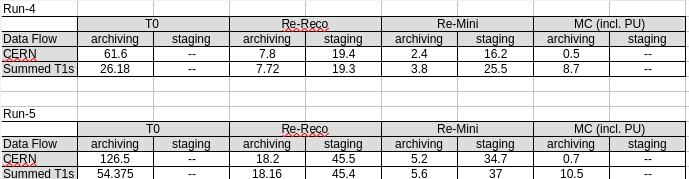
\includegraphics[width=.95\textwidth]{figs/11 Computing Infrastructure/Staging-r4r5.png}
	\begin{tabular}{|l|c|c|c|c|c|c|c|c|}
	\hline
	\rowcolor{tableheader}  Activity: & \multicolumn{2}{c|}{\TierZero}  & \multicolumn{2}{c|}{Re-Reco} 
	                                & \multicolumn{2}{c|}{Re-mini} & \multicolumn{2}{c|}{MC (incl. PU)} \\ \hline
	\rowcolor{tableheader}  Data Flow        & arch. & staging & arch. & staging & arch. & staging & arch. & staging \\ \hline    
	\cellcolor{tablerowheader}  CERN         & 71    & -       &  8    &  21     & 2     &  -      & 1     &  - \\ \hline
	\cellcolor{tablerowheader}  Sum \TierOne & 40    & -       &  8    &  21     & 4     &  26     & 8     &  - \\ \hline
	\multicolumn{9}{c}{}\\
	\end{tabular}
	\begin{tabular}{|l|c|c|c|c|c|c|c|c|}
	\hline
	\rowcolor{tableheader}  Activity: & \multicolumn{2}{c|}{\TierZero}  & \multicolumn{2}{c|}{Re-Reco} 
	                                & \multicolumn{2}{c|}{Re-mini} & \multicolumn{2}{c|}{MC (incl. PU)} \\ \hline
	\rowcolor{tableheader}  Data Flow        & arch. & staging & arch. & staging & arch. & staging & arch. & staging \\ \hline    
	\cellcolor{tablerowheader}  CERN         & 132   & -       &  18   &  46     & -     &  -      &  1    &  - \\ \hline
	\cellcolor{tablerowheader}  Sum \TierOne &  78   & -       &  18   &  46     & 6     &  42     & 9     &  - \\ \hline
	\end{tabular}
	\label{tab:staging-r4_r5}
\end{table}

 The value for an \textit{in-situ} archiving is listed for the \TierZero date export. Taking the LHC duty cycle into account would relax the value accordingly. Durations of 3 and 2 months are assumed for the Re-Reco and Re-Mini campaign examples. It should be noted that during such a campaign, staging and archiving are likely to overlap in time, and tape drives would need to be assigned for both. For the \TierOne sites, the staging capability is expected to be shared similarly to the \RunThree conditions: 40\% is provided by \gls{FNAL}, and the remaining sites contribute roughly 5--10\% each.


\subsubsection{Network resource management}

As CMS uses geographically distributed processing facilities, a robust, high-performance wide-area network is required. Significant capacity growth is expected for the educational networks by the time the \gls{HL-LHC} becomes operational. This infrastructure will serve other data-intensive research areas besides particle physics, such as the Square Kilometer Array radio telescope~\cite{ska_observatory_2021_16896182}. Dynamic bandwidth reservation at the network level is desirable to ensure controlled use of network capacity. This can be achieved through novel \gls{SDN} technology that uses dynamic programming on network routers to make the reservations. Many R\&D projects and improvements to network capabilities are coordinated through the Global Network Advancement group~\cite{gna-g.net}, where the work of the Data Intense Science group is crucial to CMS.

For example, \gls{SENSE}~\cite{Monga_2020} is software that operates across \gls{SDN} layers, controlling individual network components and the middleware used by scientific applications. During \RunThree, prototypes have been set up~\cite{Wurthwein:2022auh} to demonstrate an integration of Rucio, \gls{FTS}~\cite{Ayllon:2014wca}, and storage systems with \gls{SENSE}~\cite{sense-rucio}. Once \gls{SENSE} is deployed at the major centers for important data flows, e.g., the \gls{RAW} data archiving at \TierOne sites, dedicated bandwidth can be allocated. Services that leverage dynamic bandwidth allocation to optimize CMS data flows will need to be developed, including both technical implementation and strategies for allocating network bandwidth in an optimized way. \gls{NOTED}~\cite{NOTED} is another project that can be integrated with \gls{FTS}. CMS follows with great interest the studies and planning for evolving the network infrastructure supporting its bulk data transfers~\cite{Martelli_2015}.

In the context of the \textbf{Network.1} activity, CMS is planning to develop code to make the necessary middleware \gls{SDN}-aware. The ability to exploit dynamic bandwidth allocation via \glspl{SDN} will be evaluated during future Data Challenges (as outlined in Section.~\ref{sec:infrastructure-challenges}) with the goals to make it more efficient and to improve the predictability and scalability of the usage of finite network resources.

\subsubsection{Data management}
\label{sec:data-management}

In the original \gls{MONARC} model, each \gls{CE} was expected to be co-located with a \gls{SE} of commensurate size, under the expectation that wide-area networking would be a significant constraint. A custom data movement service, PhEDEx~\cite{Rehn2006,Tuura:2008zz}, maintained a data location catalog and moved data between sites. Over the years, the data movement functionality was replaced by the CERN \gls{FTS}~\cite{Ayllon:2014wca}, which orchestrated third-party copies between SEs via the gridftp~\cite{allcock2003,Mandrichenko2003} and, more recently, the WebDAV~\cite{Bockelman:2020isd} protocols. Meanwhile, PhEDEx did not offer data lifecycle management functionality (e.g., to implement the storage policies proposed in Tables~\ref{tab:storagepolicy1} and~\ref{tab:storagepolicy2}), leading to operational challenges as SEs filled up. To mitigate these effects, the Dynamo~\cite{dynamo} service was developed within CMS. Between \RunTwo and \RunThree, CMS reviewed its data management system and elected to migrate~\cite{toRucio} from PhEDEx+Dynamo to Rucio, originally developed within the ATLAS experiment, as it was becoming a community tool in particle physics.

The CMS Rucio migration was completed, and CMS is a significant stakeholder and provides development support for the Rucio community software. Rucio manages approximately 100 million unique CMS files grouped into about 1 million data sets. It is expected that Rucio and \gls{FTS} will both scale to meet \gls{HL-LHC} needs. The \textbf{Transfers.1} line in Table~\ref{tab:infra-rnd-table} accounts for CMS contributions to \gls{FTS} and Rucio scalability studies for scheduled bulk data transfers, including participation in the \gls{WLCG} data challenges discussed in Section~\ref{sec:infrastructure-challenges}.
For HL-LHC, CMS plans to increase both target and maximum size of data files. The current target file size of 4 \unit{GB} results in an average file size of 3\unit{GB} . The maximum size of 16\unit{GB} is set for current transfer limitations. Today's average small file size results in excessive metadata and tape writing/reading inefficiencies. For HL-LHC, the file transfer service, \gls{FTS}, needs to be enhanced with resume and multi-stream capability to efficiently transfer larger files.
These features are especially important for less well network-connected sites and storage systems. CMS envisions a target file size of 25\unit{GB}  and maximum size of 50\unit{GB} for \RunFour with plans to increase this further (by a factor two or four) for \RunFive.
Most data access from processing and analysis jobs uses the \textsc{XRootD}~\cite{CMS:2014cof} package. The software package supports the file and \textsc{XRootD} protocols, later optimized for higher-latency network-based data access. CMS also uses the package for a novel ``backup'' data access via a storage federation in case reading from the site storage fails. This greatly increases the success rate of jobs in the case of a local storage issue, reduces job failures and resubmissions, and recovers the \gls{CPU} already consumed by the job. The storage federation itself is based on \textsc{XRootD} and referred to as \gls{AAA}~\cite{Bloom:2015poa}. 

It can also be used to access a file interactively. Users like it for its simplicity: a user only needs to know the logical filename and the \gls{URL} of the entry point to the federation. CMS also relies on \gls{AAA} for serving pileup auxiliary data to \gls{MC} simulation production workflows at all CEs across the Grid. Analysis users may also rely on \gls{AAA}, depending on how they choose to run their analysis workflows. Robust scalability capabilities for \textsc{XRootD} and, by extension, for \gls{AAA}~\cite{400GbpsXRootD}, are therefore required. The \textbf{Transfers.2} activity is underway to ensure that these capabilities are available to CMS.

Successful management of the network and data transfers is predicated on a complete understanding of data flows~\cite{network-flows} and close monitoring of network utilization, particularly for unscheduled transfers such as those using \textsc{XRootD}~\cite{Garrido:2024bpi}. \textbf{Transfers.2} includes contributions and support for implementing a more comprehensive monitoring protocol for bulk data transfers using \textsc{XRootD}~\cite{Garrido:2024bpi}, resulting in greater ability to manage networking when it is properly and completely monitored.

A more speculative line of R\&D, listed as \textbf{Storage.1} in the summary table, is targeted towards leveraging the new capabilities of RNTuple (Section~\ref{sec:rntuple}) to allow data management and access at a more granular level than files in object stores~\cite{Smith:2023mrq}. The benefit of this mode of operation is that it obviates the need for data tiers by exploding files into individual event data product objects, keeping only the necessary data products available on disk. For example, CMS analysis users only access about half of the data products stored in \gls{AOD} on average~\cite{ncsmith-CHEP24}, providing significant disk savings if only the necessary data products for a given data set were stored. These data products would be stored at the page-cluster level (roughly equivalent to a TBasket in TTree) in an \gls{HTTP}-accessible object store, and referenced by \gls{URL} inside a lightweight RNTuple file, that can be used in the \gls{CMSSW} framework to provide the necessary metadata to the application.

\subsubsection{Regional data lakes}

The trend of national consolidation of computing resources is unlikely to converge on a uniform access protocol as in\gls{WLCG} CEs and SEs. It is also apparent that other science domains, whose significant computing needs drive the architecture of these infrastructures, have lower long-term storage needs than \gls{HEP}. Therefore, CMS's stakeholders must continue to provide storage and customize its architecture to ensure effective integration with each regional computing infrastructure. At the same time, the tight coupling of CEs and SEs is largely irrelevant given today’s \gls{WAN} capabilities, which suggest that a similar consolidation of storage resources may yield economies of scale. 
An illustration of the data lake concept is shown in Fig.~\ref{fig:data-lake}.

\begin{figure}
    \centering
    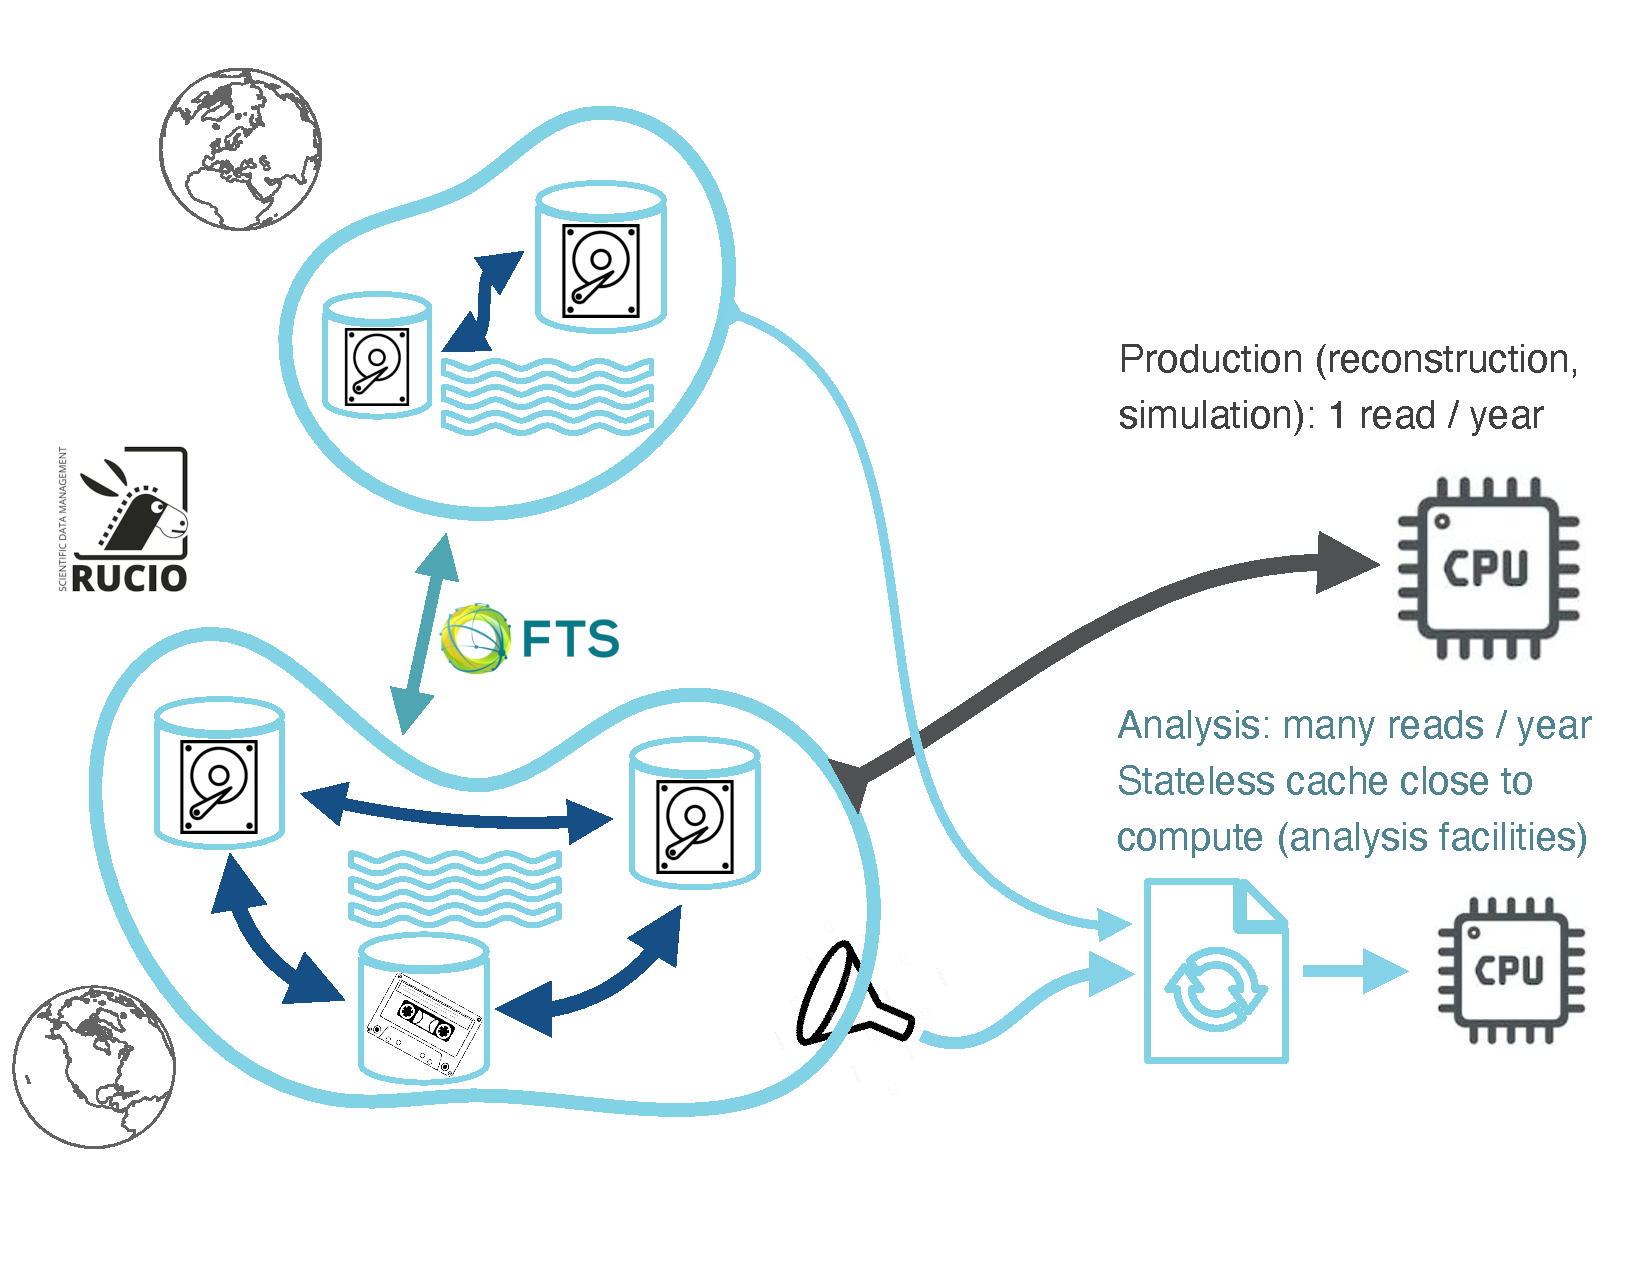
\includegraphics[width=0.7\linewidth]{figs/11 Computing Infrastructure/data-lake-diagram.pdf}
    \caption{Illustration of the data lake concept showing two geographically-separated lakes with internal disk and tape storage sites. Rucio/\gls{FTS} orchestrates transfers between lakes, while production and analysis applications stream data from the lakes. Analysis access is through a lake-edge data filtering service.}
    \label{fig:data-lake}
\end{figure}

Given the above considerations, the \gls{WLCG} Collaboration has explored ``data lake'' concepts, which consolidate storage to fewer endpoints~\cite{wlcg_datalake,wlcg_datalake_ieee}.
Currently, the contents of each of the $\approx$80 SEs in use by CMS are cataloged by Rucio, and transfers between any two are possible. With fewer endpoints, the operational burden of central data management may be reduced. One possible scenario could be the deployment of a data lake per present \TierOne site. Resources within each data lake region would still be distributed, and region-aware data and workflow management deployments would be required. The regions would have the opportunity to customize deployments according to local needs. However, significant effort would be required to transition to this approach and adapt it to each region’s specific needs. There is a risk that regions that cannot provide the required effort could become less able to participate in the experiment. In the context of the \gls{ESCAPE} project, this approach has been explored and prototyped~\cite{data_access_puzzle}.

As discussed previously, \gls{HPC} centers generally do not host \gls{WLCG} SEs, so nearby SEs must hold any input/output data, either to be transferred into/from \gls{HPC} center scratch space or streamed directly to the worker nodes. CMS has demonstrated both modes of operation in production at existing \gls{HPC} facilities. Many \gls{HPC} centers do not have high-bandwidth connections to CMS SEs either. In some cases, this is because they do not have high-bandwidth \gls{WAN} connectivity; in such cases, CMS should encourage the relevant national research network providers to improve the situation. In other cases, administrative policy precludes direct access to \gls{WAN} hosts from worker nodes. To overcome this challenge, edge services that act as caching proxies must be developed as part of the \textbf{Storage.2} activity. \gls{WLCG} experiments appear to be on the frontier of scientific data volume; it is possible that future \gls{HPC} facility designs will include capabilities to support large data flows from remote locations, as other science instruments are approaching \gls{HEP} data volumes.

%%%%%%%%%%%%%%%%%%%%%%%%%%%%%%%%
% 11.5 Analysis Infrastructure
%%%%%%%%%%%%%%%%%%%%%%%%%%%%%%%%

\subsection{Analysis infrastructure}
\label{sec-anal-in}

New software paradigms for end-user analysis were discussed in Chapter~\ref{sec:Analysis}, motivated only in part by large increases in data volumes. Expanded use of ML requires deploying specialized hardware, such as \glspl{GPU}, within the analysis infrastructure. The chapter discusses the software development and evolution of data formats, data processing, and data management needed for dedicated analysis facilities, as well as their leveraging of the wider Grid computing infrastructure. CMS will adopt a system to access analysis data on the Grid and provide CRAB functionality while adapting to the proposed analysis facilities at minimal operational cost. 

Whether specialized resources such as \glspl{GPU} at analysis facilities are included in the processing and storage pledges that federations make has implications for collaboration-wide access, interoperability, standardization of user interfaces, and whether any centrally-supported infrastructure will need to be developed and implemented. CMS also requires access to these capabilities for colleagues geographically distant from state-of-the-art analysis facilities. It is assumed that all solutions will seek to leverage the distributed computing infrastructure primarily dedicated to centralized production activities at \gls{WLCG} sites and \gls{HPC} facilities, since access to Grid compute will always be desired if dedicated analysis infrastructures become unavailable or fully occupied.

\subsubsection{Hardware aspects}

The computing infrastructure requirements for analysis listed in Section~\ref{sec:idealworkflow} address resource agnosticism and scalability, including the ability to ``burst out’’ into clusters and into the wider distributed computing infrastructure. As discussed in Section~\ref{GPU-for-analysis}, \glspl{GPU} are a requirement as well in order to enable the execution of complex machine learning models. Since resource agnosticism is required, some level of coordination of resource requests (e.g., on acceptable \gls{GPU} models) will be needed, especially if the infrastructure is shared across different experiments. At the present time, access to compute accelerators in the wider Grid infrastructure is opportunistic (unpledged) and deployment decisions are only loosely coordinated with the experiments in terms of desired models and co-location with \gls{CPU}.

Similar to modern edge services at processing facilities, the desired deployment strategy for analysis facility middleware is container-oriented. Facility designs are generally based on Kubernetes, which vastly simplifies the deployment of software systems such as JupyterHub and Dask. If analysis facilities are to be pledged, a container orchestration layer must be included in \gls{WLCG} resource definitions.

\subsubsection{Data transformation tools}

As discussed in Chapter~\ref{sec:Analysis}, there is a strong motivation for the capability of augmenting NanoAOD with new data columns extracted from (Mini-)\gls{AOD}, both from a disk usage savings perspective as well as a processing turnaround time perspective. As an illustrative use case, an analyzer may wish to add a column to all the relevant NanoAOD data sets for a low-mass scalar to diphoton search, which contains the result of a specialized diphoton \gls{DNN} evaluated on \gls{ECAL} RecHits (information only available fully in \gls{AOD}), with a turnaround time of a week. Given the regional data lake model, it is best to perform the \gls{DNN} evaluation near the mass storage, sending only the output float column to the analysis facility rather than the full input \gls{AOD}. Given that the \gls{AOD} will have to be staged from tape, this workflow is best handled by a tape-aware service, possibly queued alongside other user column extraction workflows that require the same input data. If the \textbf{Storage.1} column object R\&D were successful, this would reduce the staged volume to just the \gls{ECAL} RecHits rather than all of the \gls{AOD} data columns.

The ServiceX~\cite{Galewsky:2020xig} data transformation service is an external technology with a similar scope to the above-described requirement. ServiceX is designed to provide columnar access (to primitive data types rather than Event Data Model types) to the ATLAS xAOD data formats, with convenient user-specific column data and column caching capabilities. R\&D to extend this service to cover the MiniAOD column extraction use case is ongoing. The general thrust of work to provide a NanoAOD-as-a-service is tracked as part of the \textbf{Transfers.3} activity.

\subsubsection{Data streaming}

In contrast to the \gls{AOD} data transformation use case described previously, the MiniAOD data tier may be more widely available on disk for analysis workflows. Even though MiniAOD is significantly more compact, streaming an entire year's data and simulation to an analysis facility would saturate a 400\unit{Gbps} link for a week, though an analysis will read only a fraction of the data sets and hopefully access only a fraction of the data products therein. Given this possibility and the risk that the \textbf{Transfers.3} activity is not successful, it is prudent to ensure that high-bandwidth streaming is possible from data origins to analysis facilities in the regional data lake model. This is the motivation for \textbf{Network.2}, ensuring the storage, network, and client libraries are well-tuned to enable remote data access. As mentioned previously, operational experience with pileup data distribution and remote prompt reconstruction workflows shows that streaming is already quite reliable.

\subsubsection{Data caching for analysis}

CMS members and others are involved in R\&D efforts to address the use of caches in the distributed computing infrastructure. There have been extensive studies of caches for CMS analysis jobs at \gls{WLCG} sites in Spain~\cite{cache-ES,Dengra:2023ytr} and Italy~\cite{Tedeschi:2022swr}, as well as a cache set up between two CMS \TierTwo sites in California~\cite{cache-CA,Sim_2023}. CMS is very interested in the R\&D conducted by ESnet and partners on network caches~\cite{cache-ESnet}.

%%%%%%%%%%%%%%%%%%%%%%%%%%%%%%%%%%%%%%
% 11.5
%%%%%%%%%%%%%%%%%%%%%%%%%%%%%%%%%%%%%

\subsection{Artificial intelligence in operations}
\label{sec:infrastructure-ai}

With \gls{AI} techniques advancing by leaps and bounds in the world around us and in CMS physics analyses, the advantage of using these tools in the operation of the experiment is clear. Tasks and processes in the computing and software domain are particularly suited for such endeavors. The plans summarized below, however, depend on the rapidly evolving \gls{AI} landscape; thus, CMS must be prepared to adapt them as needed.

The techniques offer a versatile toolkit that goes beyond algorithmic automation. Most obviously, \gls{AI} enables natural-language interactions---listening, reading, writing, and even speaking---allowing operators and physicists to engage with complex systems conversationally. Less developed options, such as multimodal capabilities, go beyond text to include plots, images, audio, and video, enabling richer, more nuanced interactions than traditional tools. Swift summaries or condensations of large swaths of information are one of the strengths of \gls{AI} systems, particularly useful for distilling extensive technical logs and other documentation into concise, expert answers when time is critical. Moreover, \gls{AI} systems can execute custom actions---from verifying data consistency to automating routine checks---to support human decision-making. Finally, \gls{AI} can generate clear documentation or tutorials, ensuring that institutional knowledge is preserved and easily accessible.

The plan is to translate these functionalities into concrete applications for CMS computing and software operations, as listed below.

\begin{itemize}

\item {\em Onboarding and Training}. \gls{AI} assistants can guide new operators, computing team members, or shift takers at Point 5 or remote sites through complex procedures, reducing the steep learning curve. Expert Helper Interfaces (integrated chat-based helpers) can support both experts and casual users, offering immediate answers or links to detailed resources.

\item {\em Help Desk Support.} \gls{AI}-driven help desks can handle common inquiries efficiently, freeing human experts to focus on non-routine problems. 

\item {\em Shift Support and Logbook Analysis.} \gls{AI} agents can scan and analyze logbooks, extracting the most relevant details and providing streamlined summaries with direct links to relevant documentation or dashboards.

\item {\em Agentic Monitoring Assistance.} \gls{AI} can actively track monitoring data, highlight anomalies, and suggest pre-emptive actions, providing ``always-on'' operational awareness. 

\item {\em Automatic Software Review.} Given the large software base of the CMS experiment and the particular strength of \gls{AI} tools to analyze software repositories, operations can be optimized by automating repetitive tasks, identifying complex issues, and standardizing quality across the CMS codebase.

\end{itemize}

The strategic goal and impact of adopting \gls{AI} in CMS computing and software operations are to optimize resources, improve responsiveness, and enhance reliability. By automating routine tasks and providing predictive insights, \gls{AI} can reduce operational costs and streamline operations. So-called ``predictive service management'' becomes possible, allowing teams to resolve issues before they escalate and minimize downtime for critical data collection. Furthermore, by delivering fast, intuitive, and expert-level support, \gls{AI} elevates the overall user and ``customer'' experience---from shift operators to physicists analyzing data---ensuring that CMS remains at the forefront of efficient and innovative scientific computing.

%%%%%%%%%%%%%%%%%%%%%%%%%%%%%%%%%%%%%%
% 11.6 System Integration Challenges
%%%%%%%%%%%%%%%%%%%%%%%%%%%%%%%%%%%%%%

\subsection{Integration, testing, and benchmarking}
\label{sec:infrastructure-challenges}

Testing prototypes and deployed computing infrastructure solutions for \gls{HL-LHC} is part of the overall timeline for the \PhaseTwo upgrade, which is discussed later in Chapter~\ref{sec:Roadmap}. CMS undertook \gls{CS} challenges before \RunOne and \RunTwo with the goal of testing the functionality and scalability of the computing infrastructure. These exercises also tested offline software and physics analysis (\gls{CSA} challenges)~\cite{CSA07}. In particular, the challenge in 2014 leveraged the HammerCloud suite to execute and benchmark target achievements~\cite{vanderSter:2011zz}. There were also combined computing challenges with other experiments, for example, in 2008.

Similar exercises are already underway for the computing infrastructure. The February 2024 \gls{WLCG} data challenge~\cite{lassnig_wissing_dc2024} tested the data transfer system at 25\% of foreseen \gls{HL-LHC} scales. Further challenges are planned at the 50\% level in or around 2027 and at the 100\% level sometime after. All of these challenges had in common that the performance targets for the infrastructure and middleware were well established beforehand and subsequently met.

As countries and federations are building prototype production and analysis infrastructures, it is essential to develop methods to test the prototypes at scale before critical decision points are reached. The goal of the \textbf{Benchmark.1} activity is to develop CMS-specific and HS23-based benchmark production workflows to measure the performance of prototype computing infrastructures in general, while
\textbf{Benchmark.2} will focus on the performance of prototype computing infrastructures for analysis. Leveraging HammerCloud again, as in 2014, might be a good option, since it is a common software project with a dedicated support model. Since the current implementation of HammerCloud for CMS depends on the CRAB submission infrastructure, which will most probably be replaced on the timescale of \gls{HL-LHC} (see Chapter~\ref{sec:Analysis}), a more generalized solution would need to be developed and implemented well in advance of planned novel infrastructure deployments at scale. 

CMS will have to leverage its specific workflow and data management tools in the context of these \gls{CS} challenges. A tighter integration of the software and physics validation procedures with workflow management validation could be highly beneficial for the experiment, since leveraging the distributed computing infrastructure in such tests would exercise all areas and potentially be faster and more scalable, a necessary capability in an era of expanding numbers of microarchitectures. 

%%%%%%%%%%%%%%%%%%%%%%%%%%%%%%%%%%%
% 11.7 Summary of R\&D Activities
%%%%%%%%%%%%%%%%%%%%%%%%%%%%%%%%%%%

\subsection{Summary of R\&D activities}

Table~\ref{tab:infra-rnd-table} lists the various R\&D activities discussed in this chapter. Most have an impact on the required disk storage needed in the \gls{HL-LHC} computing model, which has been quantified and summarized in Table~\ref{tab:infra-rnd-table}. Some of the R\&D lines (e.g., \textbf{HetArch.1}, \textbf{Facilities.2}) enable quantifying the needs for \glspl{GPU} and how they might be deployed, for example, as a service. Many others enable flexibility in how resources (especially storage) are deployed and in evaluating the performance of distributed architectures. The R\&D activities will either be carried out within CMS \gls{OANDC} coordination area or, in the case of primarily external-to-CMS activities, followed by their conveners and participants.

\begin{table}[tbph]
     \centering
     \caption{Summary of infrastructure-related R\&D activities with estimated impacts and probabilities of success on the timescale of the beginning of \RunFour. Note that many of the activities have significant, or even their main, effort outside the CMS experiment.}
     \begin{tabular}{|l|c|c|c|c|} 
     \hline
     \rowcolor{tableheader}
     & Description & Impact & Prob. of &  Responsible     \\ 
     \rowcolor{tableheader}
     &             &        & Success  &  Area in \gls{OANDC}       \\
     \hline
     \hline
     \rowcolor{tableheader}
     \multicolumn{5}{c|}{\textit{Production Processing Paradigms (Section~\ref{sec:Infrastructure-Production})}} \\
     \hline
     \hline
     \cellcolor{tablerowheader}
%
HetArch.1    & CMS offline GPU    & Req. for requesting  & High &  Core Software \& \\
     \cellcolor{tablerowheader}
             & code in HEPScore   & and pledging GPU    &      &  Sub. Infra. (SI) \\
%
     \hline
     \cellcolor{tablerowheader}
Facilities.1 & Container          & Req. for efficient   & High & Facilities \&     \\
     \cellcolor{tablerowheader}
             & orchestration      & use of HPC          &      & Services          \\    
     \cellcolor{tablerowheader}
             & service (elements) & resources            &      &                   \\
% 
     \hline
     \cellcolor{tablerowheader}
Facilities.2 & Inference as a     & Req. for requesting  & High & Facilities \&     \\
     \cellcolor{tablerowheader}
             & service for recon- & and pledging GPU    &      & Services          \\   
     \cellcolor{tablerowheader}
             & struction/analysis &                      &      &                   \\
%
     \hline
     \cellcolor{tablerowheader}
Facilities.3 & Multi-node         & Alternative to       & High & Facilities \&     \\
     \cellcolor{tablerowheader}
             & scheduling         & auto-scaling for  &      & Services (with SI   \\
     \cellcolor{tablerowheader}
             &                    & GPU scheduling           &      &  \& DMWM Dev.)\\
     \hline
     \hline
%%%%%%%%%%%%%%%%%
     \rowcolor{tableheader}
     \multicolumn{5}{c|}{\textit{Dataflow and Storage Solutions (Section~\ref{sec:dataflow})}} \\
     \hline
     \hline
%%%%%%%%%%%%%%%%%
     \cellcolor{tablerowheader}
Network.1   & SDN-aware           & Req. for efficient  & High & Facilities \&  \\
     \cellcolor{tablerowheader}
            & middleware          & utilization of      &      & Services, then \\
     \cellcolor{tablerowheader}
            &                     & shared WANs under   &      & DMWM Dev. for   \\
     \cellcolor{tablerowheader}
            &                     & high demand         &      & FTS/Rucio int. \\
%
     \hline
     \cellcolor{tablerowheader} 
Transfers.1 & Rucio/FTS           & Req. for effective & High & DMWM Dev. \\ 
     \cellcolor{tablerowheader}
            & scalability         & data management    &      &            \\
%
     \hline
     \cellcolor{tablerowheader}
Transfers.2 & \textsc{XRootD} scalability, &                    & High & Facilities \& \\
     \cellcolor{tablerowheader}
            & monitoring          &  \textit{id.}      &      & Services \\
     \cellcolor{tablerowheader}
            & robustness          &                    &      &           \\
%
     \hline
     \cellcolor{tablerowheader}
Storage.1   & Individual data & More efficient          & Med. & Facilities \& \\
     \cellcolor{tablerowheader}
            & product storage & and performant use      &        & Services      \\
     \cellcolor{tablerowheader}
            & with RNTuple    & of storage resources    &        &               \\
%
     \hline
     \cellcolor{tablerowheader}
Storage.2   & Caching solution&  \textit{id.}          & High   & Facilities \& \\
     \cellcolor{tablerowheader}
            & for disk-less sites  &                    &        & Services      \\
      \hline
%
%%%%%%%%%%%%%%%%%
     \rowcolor{tableheader}
     \multicolumn{5}{c|}{\textit{Analysis infrastructure (Section~\ref{sec-anal-in})}} \\
     \hline
     \hline
%
     \cellcolor{tablerowheader}
Transfers.3 & Lake-edge data   & Req. for performant & High & Analysis       \\
     \cellcolor{tablerowheader}
            & transformation   & use of analysis     &      & Infrastructure \\
     \cellcolor{tablerowheader}
            & tools \& caching & facilities          &      & and Services   \\
     \cellcolor{tablerowheader}
            & solutions for anal- &                     &      & (AIS)          \\
     \cellcolor{tablerowheader}
            & ysis (AAA evolution) &                     &      &                \\
\hline
     \cellcolor{tablerowheader}
%
Network.2   & Networking R\&D  &   \textit{id.}      & High & AIS       \\
     \cellcolor{tablerowheader}
            & for reliable streaming    &                     &      &   \\
%
%%%%%%%%%%%%%%%%%
     \rowcolor{tableheader}
     \multicolumn{5}{c|}{\textit{System Integration Challenges (Section~\ref{sec:infrastructure-challenges})}} \\
     \hline
     \hline
     \cellcolor{tablerowheader}
Benchmark.1 & Production bench- & Req. for evaluating  & High & Computing \\
     \cellcolor{tablerowheader}
            & mark workflows    & performance of dist- &      & Operations \\
     \cellcolor{tablerowheader}
     \cellcolor{tablerowheader}
            &                   & ributed computing    &      & \\
     \cellcolor{tablerowheader}
            &                   & infrastructures      &      & \\
     \hline
     \cellcolor{tablerowheader}
Benchmark.2 & Analysis bench-   & \textit{id.}         & High & AIS \\
     \cellcolor{tablerowheader}
            & mark workflows    &                      &      &      \\
\hline
%%%%%%%%%%%%%%%%%

     \end{tabular}
     \label{tab:infra-rnd-table}
\end{table}

\clearpage

%%%%%%%%%%%%%%%%%%%%%%%%%%%%%%%%%%%%%%%%%%%%%%%%%%%%%%%%%%%%%%%%%%%%%%%%%%%%%%%%
%
% TESTING AND VALIDATION
%
%%%%%%%%%%%%%%%%%%%%%%%%%%%%%%%%%%%%%%%%%%%%%%%%%%%%%%%%%%%%%%%%%%%%%%%%%%%%%%%%
% \clearpage
% \input{tex/12_testing_validation.tex}
\section{Testing and validation}
\label{sec:Validation}


Testing and validation of CMS software are carried out at multiple levels. The initial set of tests, addressing pull requests and integration builds, has been discussed in Section~\ref{sec:buildandintegration}. This section is dedicated to the software validation process, detector condition validation, and anticipated challenges for the \gls{HL-LHC}.

A software validation process is initiated each time a new development release of \gls{CMSSW} becomes available. This includes special releases built to validate new external packages, such as \GEANTfour or \textsc{ROOT}, and to test compatibility across different architectures and operating systems. The focus of this validation can be on the physics underlying the detector simulation or on the reconstruction algorithms, ensuring that the software produces accurate and consistent results; alternatively, it can be purely technical, validating performance, stability, and compatibility with the computing environment.

Validation tasks, particularly those related to release and technical validation, are primarily handled by the \gls{OV} group, which operates under the \gls{PPD} team. Validation of the physics content of the detector simulation, often performed by comparing simulations to beam test data, falls under the responsibility of the \gls{OANDC} simulation group or the relevant \glspl{DPG}. 

\subsection{Release validation}
The central release validation is an integral part of the software development process, and serves several important purposes:
\begin{enumerate}
    \item it ensures that all software components within a release function together seamlessly, without conflicts or failures during execution;
    \item it validates the correctness of the produced physics output;
    \item it assesses and monitors the performance in terms of:
    \begin{enumerate}
        \item memory and \gls{CPU} consumption,
        \item algorithmic performance, and
        \item stability at larger scales (e.g., number of events or number of concurrent jobs).
    \end{enumerate}
\end{enumerate}

In general, release validation produces both reference and target samples, which include simulated and real data samples. Notably, the reference sample is typically the target sample from the previous validation round.

A data set centrally produced for release validation is called \gls{RelVal}. The infrastructure for preparing \glspl{RelVal} is discussed in Sec.\ref{Validation:RelValInfra}. The standard set of \glspl{RelVal} includes:
\begin{itemize}
    \item a few hundred simulated signal samples, covering both particle gun and physics processes, as well as samples with and without pileup. Each sample consists of a number of events ranging from a few thousand to hundreds of thousands, depending on the process.
    \item $\approx$100 data samples, generated by re-running the \gls{HLT}, \gls{RECO} and \gls{DQM} steps on existing \gls{RAW} data. Each sample consists of approximately 50,000 events, depending on the single-file granularity. Multiple \glspl{PD} are included, and the latest-era samples are included once available.  
\end{itemize}

This standard set is typically submitted within 24--48 hours after a new release becomes available. \gls{RelVal} production is intended to have low latency, to give developers sufficient time to validate the release and address any issues before the next iteration.

Once the \gls{RelVal} samples are produced, they are distributed to various groups, including the \gls{HLT} team, the physics groups, and the \glspl{DPG}. Central validation tools such as the \gls{DQM} \gls{GUI} and \gls{RelMon} are provided to support and streamline the validation process. The \gls{RelMon} tool automatically compares target and reference \gls{DQM} monitoring elements using predefined statistical tests, such as the $\chi^2$ test, the Kolmogorov--Smirnov test, and bin-by-bin comparisons. Based on these tests, a score is computed for each detector subsystem, and the elements failing the comparison are highlighted and available for inspection. 

Each group assigns one or more individuals, referred to as \emph{validators}, to assess whether the reference and target samples are in good agreement. Some differences can be expected due to new features introduced in updated releases, while others may indicate potential issues. In cases of problematic discrepancies, experts from the relevant subsystems conduct a detailed investigation to identify the root cause and implement fixes, if necessary. Ongoing efforts aim to automate the validation process further, for instance by integrating machine learning estimators to identify anomalous patterns and involving validators only when discrepancies are detected.

Since 2025, \glspl{RelVal} have also been employed to test the use of heterogeneous computing resources for both online and offline reconstruction. This also enables event-by-event comparisons between \gls{CPU}- and \gls{GPU}-based processing chains, enabling the monitoring and identification of potential discrepancies arising from differences in hardware architectures or numerical precision.

\subsection{Technical validation}
Technical validation focuses on assessing performance, stability, and compatibility with the computing environment. No change of physics is expected in this type of validation, which includes:
\begin{itemize}
    \item updating external packages where no physics changes are expected, e.g., the \textsc{ROOT} data analysis framework;
	\item compiling \gls{CMSSW} with different compiler versions;
    \item running \gls{CMSSW} on different operating systems;
    \item running \gls{CMSSW} on different hardware architectures, such as x86\_64 and \gls{ARM};
    \item running \gls{CMSSW} in different configurations, such as \gls{CPU}-only, \gls{CPU} and \gls{GPU}, or \gls{CPU} with remote co-processors (e.g., \gls{SONIC}).
\end{itemize}

Currently, the technical validation follows the same procedure as release validation: when \glspl{RelVal} samples become available, validators from all subsystems analyze the results and report their findings. This approach is manageable when there are only a small number of additional validation campaigns beyond release validation.
However, the number of technical validation campaigns has grown significantly in recent years, due, for instance, to an increasing number of available heterogeneous architectures and their possible configurations. To maintain a sustainable workflow, the technical validation for \gls{HL-LHC} will be automated, enabling more frequent validation cycles and earlier detection of potential issues. Automation will also enable efficient scaling of validations as the CMS software continues to evolve across diverse computing environments.

One key challenge in automatic validation is the differences in floating-point precision. Due to variations in the compiler optimizations, hardware architectures, and instruction sets (e.g., \gls{AVX} vs. \gls{SSE}), numerical results may not be bitwise identical across different configurations. These small discrepancies, often limited to the least significant digits, can cause statistical tests (e.g., $\chi^2$, Kolmogorov--Smirnov) to detect differences that are not physically meaningful. To address this, validation frameworks will incorporate tolerance thresholds or probabilistic comparisons, ensuring that minor numerical variations do not trigger unnecessary warnings while still identifying significant discrepancies.

\subsubsection{Infrastructure for \glspl{RelVal} workflow}
\label{Validation:RelValInfra}
During \RunThree, a dedicated infrastructure was deployed for \gls{RelVal} workflows, to ensure a fast turnaround. Its purpose is to ensure these workflows execute efficiently and promptly, even when the rest of the system is under high load or contention. This setup is essential for maintaining continuous validation of software releases and providing rapid feedback to developers. The fundamental components of this infrastructure are:
\begin{enumerate}
    \item a \emph{dedicated WMAgent:} \gls{RelVal} workflows are managed by a separate WMAgent instance. This \gls{RelVal} WMAgent exclusively pulls \gls{RelVal} workflows, creating and submitting their jobs to HTCondor; when the other WMAgents managing production workflows are busy, the \gls{RelVal} WMAgent remains unaffected;
    \item a \emph{priority system:} release validation jobs have the highest scheduling priority among production jobs. Only two types of jobs can take precedence over \gls{RelVal} jobs in HTCondor: \TierZero jobs for prompt reconstruction of detector data and so-called \emph{high-prio} jobs, used by administrators for small-scale tests;
    \item \emph{sites:} \gls{RelVal} jobs are executed at the largest and most reliable CMS computing sites, which are, since 2025, the CERN \TierTwo and the \gls{FNAL} \TierOne and, for \gls{RelVal} running on heterogeneous resources, the KIT \TierOne and the University of Wisconsin \TierTwo.
\end{enumerate}

\paragraph*{Failure handling and resubmissions}

\gls{RelVal} jobs can be automatically retried by the WMAgent in case of failure. The retry behavior — including whether a failed job should be retried, the maximum number of retries allowed, and the waiting or \textit{cooloff} period between retries — is fully configurable within WMAgent. In contrast to simulation or ReReco workflows, once all jobs of a \gls{RelVal} workflow have completed, the workflow is automatically \emph{announced}, i.e., ready to be used, even if some output data sets are missing a fraction of the expected statistics.

\paragraph*{Relval output data placement}
Up until 2024, most of the \gls{RelVal} outputs were stored at CERN. However, this data placement model consumed more than 25\% of the total storage resources allocated for central production needs at the CERN \TierTwo site. This situation made space management increasingly challenging, leading to a revision of the \gls{RelVal} output policy. According to the new policy, only specific data tiers such as \gls{GEN} and \gls{GEN}-\gls{SIM} are now kept at CERN and \gls{FNAL}, while all remaining data tiers are stored at other sites with two replicas.


Before this policy change, \gls{RelVal} outputs were managed by an ad-hoc \gls{WM} microservice called \texttt{MSOutput}. Since then, the management of \gls{RelVal} outputs has been fully migrated to the Rucio subscriptions mechanism, which provides more flexible and expressive data placement rules without requiring additional development.

The overall size of \gls{RelVal} data sets for a single validation campaign can vary from $\mathcal{O}(100\;\text{GB})$ to $\mathcal{O}(100\;\text{TB})$, depending on the validation purpose. 

The primary event content formats used for \gls{RelVal} workflows are \gls{FEVT}, \gls{DQM}, and \gls{GEN}-\gls{SIM}, described in Chapter~\ref{sec:Model}. All \gls{RelVal} samples are kept on disk for a minimum of three months. \gls{DQM} samples are stored indefinitely to preserve the history of validation results, while \gls{GEN}-\gls{SIM} samples are stored for up to one year to serve as inputs for further workflows or for \gls{PU} mixing.

\paragraph*{Resource requirements}
Similar to production workflows, \gls{RelVal} workflows are configured before submission to meet their resource requirements. The submitter defines how many \glspl{CPU} and how much memory are required. Similarly, the submitter also provides a time estimate for the time required to produce one event. \gls{CPU} and memory requirements are used to allocate resources for \gls{RelVal} jobs in HTCondor. The time-per-event estimate is used to determine how many events a Grid job must produce to achieve the target wall-clock time of 8 hours. \gls{RelVal} workflows by default uses 8 \gls{CPU} cores, 16\unit{GB} memory and 1 second time-per-event. 

\paragraph*{Current shortfalls and planned improvements for \PhaseTwo}
For rapid completion of \gls{RelVal} workflows, input samples must be available on disk. Currently, workflows injected into the \gls{WM} system automatically stage their inputs; if data is on tape, staging can take up to a few days. During \RunThree, manual pre-staging by the \gls{OV} group via a dedicated Rucio account enabled staging data to CERN and \gls{FNAL}, but this approach is labor-intensive. In addition, workflows may have been injected before inputs are ready, causing delays. An automated pre-staging mechanism is currently under development and testing, and will use data set pinning for inputs already required by \gls{RelVal} workflows. This approach would limit delays to the first workflow injection, significantly improving subsequent \glspl{RelVal} turnaround.

One current limitation of \gls{RelVal} workflows is that a single WMAgent must execute them at a single site. This restriction arises because each \gls{RelVal} workflow includes a \emph{harvesting} step for jobs to read the \gls{DQM} data sets produced by the workflow and generate flat \textsc{ROOT} files containing the final histograms. These are compared via the \gls{RelMon} system and inspected by the validators. The files are then uploaded to the \gls{DQMGUI} server. If a \gls{RelVal} workflow were to run across multiple sites, harvesting jobs at different sites could potentially overwrite each other's outputs on the \gls{DQMGUI} server. Similarly, if a workflow were managed by multiple agents, harvesting jobs under different agents could interfere with one another, resulting in only partial \gls{DQM} uploads. This limitation needs to be addressed in \PhaseTwo.

In Section~\ref{sec:wm_sys_integration}, the two modes of workflow execution, TaskChain and StepChain, are described. In the current \RunThree system, \gls{RelVal} workflows can only be executed as TaskChain. Production workflows have demonstrated faster turnaround times when run in StepChain mode. Reviewing the constraints that currently prevent \gls{RelVal} workflows from using StepChain, and evaluating the feasibility of enabling them to run in this mode for improved turnaround, are the subject of an R\&D activity for \PhaseTwo.

\subsection {Conditions validation}
Conditions data is non-event data derived from calibration and alignment algorithms. This data is fundamental to correct the detector response to be uniform in space (i.e., across different regions of the detector) and in time, when the radiation absorbed by the detectors changes their response. Condition data is composed of three basic entities:
\begin{enumerate}
    \item payload: the fundamental unit of conditions data, representing a set of parameters used in physics data processing workflows;
    \item \gls{IOV}: the time range during which a specific payload remains valid;
    \item tag: a fully qualified set of payloads and associated \glspl{IOV}, covering the required time span for a given workflow.
\end{enumerate}

Each \gls{DPG} continuously updates its detector calibrations during data taking and provides them as candidate tags, which must be validated before being applied to physics data. During \RunThree, this validation is performed in two modes:
\begin{itemize}
    \item \textbf{Full Track Validations (FTV)}: these are requested by the groups when major updates are introduced in a new tag candidate, reflecting the latest detector evolutions. Such updates may include new alignments, response corrections, or significant threshold modifications, and may involve conditions used at the \gls{HLT}. In this case, the validation procedure is similar to that used for release validations. A set of data samples is produced for a selected list of data sets using both the current reference conditions and the conditions to be tested. Submission follows the same workflow as \glspl{RelVal}. The final \gls{DQM}-based comparison is provided to experts in the relevant \glspl{DPG} and \gls{HLT} group, and the results are validated.
    \item \textbf{Fast Track Validations (FAST)}: For minor updates, such as adjustments to faulty components or updates to electronic maps, the validation is restricted to ensuring that the new conditions do not induce failures in data-taking jobs on the \gls{HLT} and \gls{DQM} nodes.
\end{itemize}

The most critical aspect of conditions validation is the strict time constraint. To ensure smooth operations, some validations must be completed within 48 hours of data collection, in time for prompt reconstruction. To reduce duplication and simplify maintenance, the FTV submission infrastructure is being integrated with the \gls{RelVal} infrastructure.

Another major challenge is preparing conditions to simulate the CMS detector response to physics particles accurately throughout the data-taking year. Currently, CMS applies average detector effects over an entire run year. During \gls{HL-LHC}, certain detector conditions may evolve significantly over time, demanding a more dynamic approach. Examples include, 
\begin{itemize}
    \item radiation-induced degradation in the pixel detector or electromagnetic calorimeter, or
    \item increasing dead areas in detector subsystems over prolonged operation. 
\end{itemize}
A straightforward approach to handling these effects is to organize multiple \gls{MC} simulation production campaigns per year, each representing a period during which average conditions remain valid. However, this approach is not sustainable in the long term, as it requires,
\begin{itemize}
    \item An increasing number of \gls{MC} simulation production campaigns,
    \item A growing number of pileup libraries,
    \item Redundant efforts in preparing simulation requests.
\end{itemize}
To address these challenges, CMS has already explored a ``Run-Dependent'' simulation campaign approach, in which a single simulation request can encompass the entire data-taking year. This would be achieved by weighting different detector conditions according to the integrated luminosity ratio of each period, ensuring a more accurate and scalable simulation strategy for \gls{HL-LHC}. This approach has already proven effective for \gls{ECAL} simulation but needs to be extended to other detectors and finalized by optimizing the required resources.

\subsection {Validation of simulated samples}
Validation of simulated samples is performed in two different cases. The first is when CMS transitions to a major \GEANTfour release. In this case, validation consists of comparing energy distributions produced by isolated charged hadrons in CMS proton-proton collisions with predictions from different \GEANTfour physics models. 

The second case involves using real collider samples for specific years to validate large samples of simulated events. The purpose is to verify agreement across low-level and high-level physics objects, covering all reconstructed physics quantities. The two validation exercises described here rely on the \gls{RelVal} infrastructure, and do not pose significant challenges in preparation for \gls{HL-LHC}. 
Success, however, depends strongly on community support for the physics model development and validation work performed within the \GEANTfour Collaboration. 


\clearpage

%%%%%%%%%%%%%%%%%%%%%%%%%%%%%%%%%%%%%%%%%%%%%%%%%%%%%%%%%%%%%%%%%%%%%%%%%%%%%%%%
%
% COMPUTING RESOURCE ESTIMATES AND PROJECTIONS
%
%%%%%%%%%%%%%%%%%%%%%%%%%%%%%%%%%%%%%%%%%%%%%%%%%%%%%%%%%%%%%%%%%%%%%%%%%%%%%%%%
% \clearpage
% \input{tex/13_resource_estimates.tex}
\section{Computing resource estimates and projections}
\label{sec:EvilPlots}

The CMS computing model was outlined in Chapter~\ref{sec:Model} and includes data formats and event sizes, a description of the tiered computing resource model, strategies for data processing and storage, network specifications, and requirements for high-fidelity simulation events. 

To provide quantitative predictions of computing resource needs (\gls{CPU}, disk, and tape) and to steer R\&D efforts toward the greatest benefit, a simulation of the computing model has been developed over the years. The primary drivers of these predictions are the LHC and CMS running conditions, the CMS offline software, and the physics analysis needs. These inputs include the running plan for proton-proton and heavy ion collisions; how much detector data and \gls{MC} simulation is needed; how and when should these data be processed; the compute time it takes to process the data through the production chain and analysis; the size of each data tier; and how long each data tier should be available on disk and retained on tape.

This chapter describes the methodology used to perform the computing model simulation and presents its predictions for a baseline scenario and several other scenarios that depend on the degree of success and adoption of various lines of research.

\subsection{LHC running conditions}
\label{sec:LPC}

Certain input parameters for the simulation of the computing model were defined and provided by the \gls{LPC}, including the LHC center-of-mass energy, the average pileup, the integrated luminosity collected per year, the live time for proton-proton and heavy-ion running, and the type of ions to be collided. The baseline scenario for \RunFour and \RunFive, as provided by the \gls{LPC}~\cite{edms:lhc_parameters}, is shown in Table~\ref{tab:LPC-inputs}.
\RunFour is planned to last 3.5 years, until the end of 2033, and \RunFive 5.5 years, until the end of 2041, with an \gls{EYETS} of 20 weeks starting by the end of Q4 in 2039 and extending into 2040.

The luminosity numbers are intended to be with ``leveling'', a technique that allows the collider to operate at a constant luminosity below the maximum possible virtual value. Because this leveling is expected for most of a fill, the luminosity, and thus pileup, is considered to be constant at the leveling value for all the duration of a fill for the purpose of resource projections.

In this CDR, CMS adopted the LHC running conditions distributed by the CERN management to all experiments in July 2025. The nominal conditions considered in this document are 150 pileup interactions in \RunFour and 200 pileup interactions in \RunFive. Sensitivity studies use variations with 150 or 200 pileup interactions in both runs. 
The total integrated luminosity over all LHC runs is assumed to reach 3\,000\fbinv. 

\begin{table}[tbph]
    \centering
    \caption{Input parameters to the simulation of the computing model from the \gls{LPC} group, with baseline values for \RunFour and \RunFive. The instantaneous luminosity, pileup and integrated luminosity are lower than the values quoted for the first year of \RunFour and \RunFive. }
    \begin{tabular}{|l|c|c|}
    \hline
    \rowcolor{tableheader}     Parameter                            & \RunFour        &   \RunFive \\ \hline 
    \cellcolor{tablerowheader} Energy pp [TeV]                      & \multicolumn{2}{c|}{14}     \\ \hline
    \cellcolor{tablerowheader} Luminosity [$10^{34}$\percms]        & 5.6            & 7.5        \\ \hline
    \cellcolor{tablerowheader} Average pileup                       & 150            & 200        \\ \hline
    \cellcolor{tablerowheader} Avg. int. luminosity / year [\fbinv] & 260            & 350        \\ \hline
    \cellcolor{tablerowheader} Livetime pp / year [Ms]              & 6.7            & 7.5        \\ \hline
    \cellcolor{tablerowheader} Livetime HI / year [Ms]        & \multicolumn{2}{c|}{1.25}   \\ \hline
    \cellcolor{tablerowheader} HI run type                    & \multicolumn{2}{c|}{Pb-Pb}  \\ \hline
    \end{tabular}
    \label{tab:LPC-inputs}
\end{table}

\subsection{CMS running conditions}
\label{sec:cmsrunning}

It should be noted that the CMS \gls{DAQ} \gls{TDR}~\cite{CMS:2021DAQTDR}, published in 2021, presents a baseline scenario of 5\unit{kHz} for the (prompt reconstructed) \gls{HLT} rate in \RunFour and 7.5\unit{kHz} in \RunFive, based on extrapolations of the rate needed for the CMS physics program during \RunTwo. The experience of \RunThree has shown that a total rate of over 10\unit{kHz} has been achieved, corresponding to about 3\unit{kHz} promptly-reconstructed and 7\unit{kHz} parked. It has been estimated that in \RunFour there will be no technical showstopper for CMS to achieve a 10\unit{kHz} HLT rate, or even higher figures (up to 15\unit{kHz}), provided a modification of the budgetary constraints. For this document, a total \gls{HLT} rate of 10\unit{kHz} (\RunFour) and 15\unit{kHz} (\RunFive) is taken as a central value for the computing model, with an HLT scouting rate of 150 (225)~kHz for \RunFour (\RunFive), corresponding to 30\% of the \gls{L1T} rate of 500 (750)~kHz. The 5\unit{kHz} CMS baseline is included in the parameter variation studies. These variations with respect to the central-value-based computing model, also shown in Table~\ref{tab:CMS-inputs}, are considered to study resilience and sensitivity to model inputs. 

\begin{table}[tbph]
    \centering
    \caption{ CMS-specific input parameters to the simulation of the computing model, with baseline values for \RunFour and \RunFive. The quoted \gls{HLT} trigger rates, shown with an ($*$), are presented as the most likely central values and are shifted relative to the CMS official baseline presented in the \gls{DAQ} \gls{TDR}. The variations are used to measure the model’s sensitivity to uncertainties in the baseline or central-value inputs. Parameters are divided into sets corresponding to trigger rates, data processing model choices, event sizes, and event processing timing. For completeness, the different pileup scenarios of the LHC in \RunFour and \RunFive are also given.}
    \begin{tabular}{|l|c|c|c|c|}
    \hline
    \rowcolor{tableheader}                Parameter             &  \RunFour      &   \RunFive     &     Variation        & Reference  \\ \hline
    \rowcolor{tableheader}                  \multicolumn{5}{c|}{LHC}                                                  \\ \hline 
    \cellcolor{tablerowheader} Average pileup                   &     150     & 200 &   both 150, both 200             & Section~\ref{sec:LPC} \\ \hline
    \rowcolor{tableheader}                  \multicolumn{5}{c|}{Trigger Rates}                                                  \\ \hline 
    \cellcolor{tablerowheader} HLT Rate [kHz]                   &     10$^{*}$      &    15$^{*}$       &      $\pm50\%$       & Section~\ref{sec:cmsrunning} \\ \hline
    \cellcolor{tablerowheader} HLT Scouting Rate [kHz]  & 150   & 225 &  $\pm50\%$    &     Section~\ref{sec:scouting}       \\ \hline
    %\cellcolor{tablerowheader} L1 Scouting Rate [kHz]          &  &   &    &    Section~\ref{sec:scouting}         \\ \hline
    \rowcolor{tableheader}                  \multicolumn{5}{c|}{Data Processing, Physics}                                       \\ \hline
    \cellcolor{tablerowheader} Req. MC events / \fbinv &\multicolumn{2}{c|}{$4.8\times10^{8}$}&    $\pm$50\%               & \multirow{3}{*}{Section~\ref{sec:Simulation}} \\ \cline{1-4}
    \cellcolor{tablerowheader} \textsc{FastSim}/\textsc{FlashSim} Fraction        &\multicolumn{2}{c|}{0\%}   &  +75\%       &            \\ \hline
    \cellcolor{tablerowheader} Prompt Reconstruction Fraction   &\multicolumn{2}{c|}{100\%}  &      30\%-100\%      & \multirow{3}{*}{Section~\ref{sec:dataprocessing}} \\ \cline{1-4}
    \cellcolor{tablerowheader} PCL Delay                      &\multicolumn{2}{c|}{48 hours}&       2--21 days      &            \\ \cline{1-4}
    \cellcolor{tablerowheader} Reprocessing Passes per Year       &\multicolumn{2}{c|}{1}     &          0           &            \\ \hline
    %\cellcolor{tablerowheader} \gls{RAW}$^\prime$ Fraction pp         &\multicolumn{2}{c|}{0\%}   &  in R\&D scenarios       & Section~\ref{sec:rawprime} \\ \hline
    \rowcolor{tableheader}          \multicolumn{5}{c|}{Event Processing Timing [HS23-s]}                                 \\ \hline 
    \cellcolor{tablerowheader} GEN                          & \multicolumn{2}{c|}{523} &    +50\%           & \multirow{2}{*}{Section~\ref{sec:dataprocessing}} \\ \cline{1-4}
    \cellcolor{tablerowheader} SIM                          & \multicolumn{2}{c|}{543} &  +50\% & \multirow{2}{*}{Section~\ref{sec:dataprocessing}} \\ \cline{1-4}
    \cellcolor{tablerowheader} DIGI  &    460   &    573 &        +50\%         &            \\  \cline{1-4}
    \cellcolor{tablerowheader} RECO      &    1\,086    &   1\,745 &        +50\%         &            \\
    \hline
    \cellcolor{tablerowheader} HLT Scouting Post-Processing     &             &             &        +50\%         &            \\ \hline
    %\cellcolor{tablerowheader} L1T Scouting Post-Processing      &             &             &        +50\%         &            \\ \hline
    \rowcolor{tableheader}                      \multicolumn{5}{c|}{Event Sizes [kB]}                                           \\ \hline 
    \cellcolor{tablerowheader} RAW                              &    4\,600    &    5\,900    &        +50\%         & \multirow{6}{*}{Section~\ref{sec:dataformats}} \\ \cline{1-4}
    \cellcolor{tablerowheader} AOD(SIM)                         &    1\,500    &    2\,000    &        +50\%         &            \\ \cline{1-4}
    \cellcolor{tablerowheader} MiniAOD(SIM)                     &     190     &     250     &        +50\%         &            \\ \cline{1-4}
    \cellcolor{tablerowheader} NanoAOD(SIM)                     &\multicolumn{2}{c|}{4}     &        +50\%         &            \\ \cline{1-4}
    \cellcolor{tablerowheader} HLTScout                         &      25     &      32     &        +50\%         &            \\ \cline{1-4}
    %\cellcolor{tablerowheader} L1Scout                          &             &             &        +50\%         &            \\ \cline{1-4}
    \rowcolor{tableheader}                       \multicolumn{5}{c|}{Data Replication Policy}                                   \\ \hline 
    \cellcolor{tablerowheader} RAW replicas on tape             &\multicolumn{2}{c|}{1.5}   &       1.0--2.0        & Section~\ref{sec:datastorage} \\ \hline
    \end{tabular}
    \label{tab:CMS-inputs}
\end{table}

\subsection{Effects of R\&D activity on resource needs}
\label{sec:overallRDimpact}

Table~\ref{tab:effects-of-rnd} contains a list of those R\&D efforts which have an impact on event timings, sizes for core software improvements (Table~\ref{tab:fwk-improvements}), generation (Table~\ref{tab:gen-improvements}), detector simulation (Table~\ref{tab:sim-improvements}), and reconstruction (Table~\ref{tab:reco-improvements}). Efforts to offload tasks to \glspl{GPU} have a large impact on the data processing strategy and computing infrastructure, as do activities to reduce the number of fully simulated events needed, and are also listed in Table~\ref{tab:effects-of-rnd}. 

The lower of the success and adoption probabilities of each of the activities is considered for the purposes of Table~\ref{tab:effects-of-rnd}, and mutually exclusive lines are indicated by a dagger (\dag). Three compound scenarios from Table~\ref{tab:effects-of-rnd} are constructed to estimate the effects of R\&D activities: one for which only those of high probability of success and adoption (H) are considered, a second scenario in which those of medium probability are included (H+M), and a third scenario where all the R\&D lines achieve their goals regardless of their success probabilities (H+M+L). 

\begin{table}[tbph]
    \centering
    \caption{Impacts of R\&D activities on resources: event size, number of fully simulated events needed, \gls{CPU} time per event for generation (\gls{GEN}), detector simulation (\gls{SIM}), and reconstruction (\gls{RECO}). The impact amount is expressed as the percentage of the total \gls{CPU} time/storage that is saved, or the \gls{CPU} time fraction offloaded to \glspl{GPU}, for the relevant module or data tier. Activities without a direct numerical impact on the resource estimates are not included. The probability of success or adoption is taken as the lower of the two. Mutually exclusive lines are indicated by a dagger (\dag).}
    \begin{tabular}{|l|c|c|c|}
    \hline
    \rowcolor{tableheader}  R\&D Activity         & Probability & Module or                     & Amount (\%) of total for module (GEN,\\ 
    \rowcolor{tableheader}                        &             & Data Tier                     & SIM, RECO) or data tier (RAW, RECO)\\    
    \hline
    \cellcolor{tablerowheader} Gene.1             &      H      &  GEN                    & -10\% (CPU mean of mix) \\  \hline
    \cellcolor{tablerowheader} Gene.2             &      H      &  GEN                    & -15\% (CPU mean of mix) \\ \hline
    \cellcolor{tablerowheader} Gene.3             &      M      &  GEN                    & 3.4 less \textsc{Madgraph} evts. \\ \hline
    \cellcolor{tablerowheader}                    &      H      &  GEN                    & -15\% \textsc{Madgraph} (CPU)  \\  
    \cellcolor{tablerowheader} Gene.4             &      H      &  \gls{GEN}                    & 80--95\% \textsc{Madgraph} LO CPU on GPU \\ 
     \cellcolor{tablerowheader}                   &      M      &  GEN                    & 50--70\% \textsc{Madgraph} NLO CPU on GPU \\  \hline 
    \cellcolor{tablerowheader} Gene.5             &      L      &  GEN                    &   90\% \textsc{Madgraph} (ML) \gls{CPU} to GPU                     \\ \hline
    \cellcolor{tablerowheader} Simu.1             &      H      &  SIM                    & -25\% \textsc{FullSim} (CPU) \\ \hline
    \cellcolor{tablerowheader} Simu.2             &      H      &  SIM                    & -50\% \textsc{FullSim} (CPU) \\ \hline
    \cellcolor{tablerowheader} Simu.3             &      M      &  SIM                    & 50--75\% G4 CPU on GPU (\RunFour) \\ \hline
    \cellcolor{tablerowheader} Simu.4             &      M      &  SIM                    & 75--95\% G4 CPU on GPU (\RunFive)\\ \hline
    \cellcolor{tablerowheader} Simu.5\dag         &      H      &  SIM                    &  -15\% \textsc{FullSim} evts. to parametric \textsc{FastSim}  \\ \hline
    \cellcolor{tablerowheader} Simu.6\dag         &      M      &  SIM                    & -50\% \textsc{FullSim} evts. to \textsc{MLFastSim} \\ \hline
    \cellcolor{tablerowheader}  Simu.7a           &      M      &  SIM                    &   \textsc{MLFullSim}: 65\% \textsc{FullSim} CPU on GPU   \\  \hline
    \cellcolor{tablerowheader}  Simu.7b           &      M      &  SIM                    &   \textsc{MLFastSim}: 50\% \textsc{FastSim} CPU on GPU   \\  \hline
    \cellcolor{tablerowheader} Simu.8\dag         &      L      &  SIM                    & -25\% \textsc{FullSim} evts. to \textsc{FlashSim}\\ \hline
    %\cellcolor{tablerowheader} Simu.8            &      H      &  \gls{SIM}                    &   0 \textcolor{red}{negligible?}   \\  \hline % FIXME: to be changed according to the new approach for Simu.8
    \cellcolor{tablerowheader} Simu.9\dag
    %\rotatebox[origin=c]{270}{$\Lsh$}
                                                  &      L      &  SIM                    & 90\% \textsc{FlashSim} CPU on GPU \\ \hline
    \cellcolor{tablerowheader} Simu.11\dag        &      L      &  SIM                    &   50\% DIGI CPU on GPU    \\ \hline
    \cellcolor{tablerowheader} Simu.12            &      L      &  SIM                    &   -90--100\% premix data set size   \\ 
    \cellcolor{tablerowheader}                    &      L      &  SIM                    &   +3--13$\times$ DIGI CPU    \\ \hline
    \cellcolor{tablerowheader} Reco.1             &      H      &  RECO                   & -50\% continuous total (CPU) \\ \hline
    \cellcolor{tablerowheader} Reco.2             &      H      &  RECO                   &  -80\% vertex vectoriz. (CPU)\\
    \cellcolor{tablerowheader}                    &      H      &  RECO                   & $>$90\% CPU on GPU\\ \hline
    \cellcolor{tablerowheader} Reco.3             &      H      &  RECO                   &  -60\% pixel-track seeding CPU \\
    \cellcolor{tablerowheader}                    &      H      &  RECO                   &  $>$90\% CPU on GPU \\ \hline 
    \cellcolor{tablerowheader} Reco.4a\dag\dag    &      H      &  RECO                   &  -65\% mkFit vectoriz. (CPU) \\ \hline
    \cellcolor{tablerowheader} Reco.4b\dag\dag    &      H      &  RECO                   & -45\% mkFit/LST CPU to GPU \\ \hline
    \cellcolor{tablerowheader} Reco.5a\dag        &      H      &  \gls{RECO}                   & $>$90\% HGCAL TICL CPU to GPU \\ \hline
    \cellcolor{tablerowheader} Reco.5b            &      H      &  RECO                   & $>$ 90\% particle-flow CPU to GPU \\ \hline
    \cellcolor{tablerowheader} Reco.6             &      M      &  RECO                   & $>$90\% elec. CPU on CPU \\ \hline
    \cellcolor{tablerowheader} Reco.7             &      M      &  RECO                   &  $>$90\% particle-flow ML-based CPU to GPU \\ \hline 
    \cellcolor{tablerowheader} Reco.8         &      M      &  RECO                   &  $>$90\% CPU to GPU \\ \hline    

    \cellcolor{tablerowheader} Reco.9a\dag\dag    &      L      &  RECO                   & $>$90\% mkFit/LST + 5\% of total CPU time  \\ 
    \cellcolor{tablerowheader}                    &             &                               &  for additional tracking step CPU to GPU \\ \hline

    \cellcolor{tablerowheader} Reco.9b            &      L      &  RECO                   & -5\% MTD CPU to GPU \\ \hline
    \cellcolor{tablerowheader} Reco.9c            &      L      &  RECO                   & -5\% muon CPU to GPU \\ \hline
    \cellcolor{tablerowheader} Reco.9d            &      L      &  RECO                   & -2\% from other algorithms CPU to GPU \\ \hline
    
    \cellcolor{tablerowheader} DataF.1            &      M      &  RAW                    & -30\% (event) size\\ \hline
    \cellcolor{tablerowheader} DataF.2            &      H      &  AOD \& derived         & -15\% (event) size\\ \hline
    \cellcolor{tablerowheader} DataF.3            &      H      &  AOD                    & -50\% (data set) size\\ \hline
    \end{tabular}
    \label{tab:effects-of-rnd}
\end{table}

\subsubsection{R\&D to improve computing infrastructure}

The actual resource needs are driven by the input parameters to the computing model, such as event sizes, logging rate, the required number of simulation events, the number of file replicas, and assumptions about turnaround times for certain workflows. Infrastructure improvements are primarily aimed at developing cost-effective solutions. Another important aspect is the required effort to operate infrastructure and R\&D exploring solutions towards the use of infrastructures that are shared with other \gls{HEP} experiments or with neighboring fields.

Other R\&D targets the selection of appropriate hardware solutions that deliver the required performance for minimal investment. Particularly in the realm of mass storage, there is a large parameter space to trade between capacity, \gls{IO} performance, or data safety. Similarly, R\&D on SDNs and related data management middleware will allow for an optimised procurement of network bandwidth and a controlled usage of research networks that is expected to be shared with other data-intense sciences in the future. However, it is very difficult to quantify savings because operational costs for shared infrastructure can vary from country to country.

\subsubsection{R\&D to reduce \gls{CPU} time and storage needs}

The total \gls{CPU} time savings from continuous improvements coming from, e.g., \textbf{gene.1}, \textbf{simu.1}, \textbf{reco.1}, was estimated as $1-X$, where $X$ is the overall reduced time for the module expressed as a fraction of the pre-R\&D measurement. The value $X$ is calculated as $(1-x)^n$, where $x$ is the time savings fraction per year and $n$ is the number of years left before the start of \RunFour. For each R\&D scenario, the compound \gls{CPU} or event size impact for each software module (\gls{GEN}, \gls{SIM}, \gls{DIGI}, \gls{RECO}) or data tier is calculated using similar expressions as for the continuous time improvement, $1-Y$ and $\prod(1-y_i)$, where $Y$ is the total reduced time (size) for the module (event) after R\&D expressed as a fraction of the pre-R\&D measurement, and $y_i$ is the \gls{CPU} (storage) savings for activity $i$ expressed as a fraction of the time (storage) spent before R\&D. The compound impact values for the three R\&D scenarios are used to make variations to the baseline scenario of ``No R\&D'' in the resource needs projections.

Many but not all of the R\&D activities in the previous chapters have a beneficial impact on metrics such as time per event, event size, or data set size. For example, solving the negative weights problem in event generators (\textbf{gene.3}) does not affect event timings or sizes, but rather the required number of \textsc{Madgraph\_MC@NLO} events, which would decrease by up to a factor of 3.4. This reduction would result in the \textsc{Madgraph} contribution to the total falling from 37\% to 15\%, equivalent to 178\unit{Mevts/\fbinv} and 52\unit{Mevts/\fbinv}, respectively. 
The activities focused on data formats target a reduction in the size of the \gls{RAW} event content(\textbf{DataF.1}), the event size in derived reconstructed data formats (\textbf{DataF.2}), and the size of the AOD data sets (\textbf{DataF.3}). The \textbf{Simu.12} effort to generate pileup and do mixing on-the-fly has a significant impact on storage needs, since it eliminates the need of a pileup library.
Other R\&D activities, such as \textbf{Simu.5}, \textbf{Simu.6}, \textbf{Simu.7a/b}, and \textbf{Simu.9}, have the effect of enabling the use of fast simulation tools such as \textsc{FastSim}, \textsc{MLFullSim}, \textsc{MLFastSim}, or \textsc{FlashSim}, and increase the fraction of simulation events processed with them. Likewise, offloading to \glspl{GPU} does not necessarily affect the overall computational budget but rather where that budget is spent, either on \glspl{CPU} or \glspl{GPU}, and is not discussed here but in Section~\ref{sec:effect-GPU}. 
The impacts of reconstruction activities for the three compound R\&D scenarios were calculated in the same way as for generator and detector simulation activities, using the measured fractions of total reconstruction time for each sub-module provided in Table~\ref{tab:recoTiming}. For the pixel-track seeding code, the assumption is that it uses $1/4$ of the tracking time (12\% of the total \gls{RECO} time), while mkFit uses approximately 20\% (10\%).

The middle scenario is split into two, (H+M) and (H+M)$^\prime$, to allow for two detector simulation options based on which medium-probability simulation R\&D activities are deemed successful. Scenario (H+M) focuses on moving \textsc{FullSim} to \gls{GPU} via both classical and \gls{ML} approaches, while scenario H+M$^{\prime}$ focuses on improvements to \textsc{FastSim}, including \gls{GPU} usage via \gls{ML}; these two solutions, based on the success of high and medium-probability R\&D lines, are considered to be exclusive, either opting for one or the other. The high-probability scenario only includes incremental \gls{CPU}-based improvements to \textsc{FullSim} and \textsc{FastSim}, while the low-probability scenario uses \textsc{FlashSim} for 25\% of events, \textsc{MLFastSim} for 50\% of events, and \textsc{MLFullSim} for 25\% of events, with components of all simulation engines running on \glspl{GPU}.

In summary, four scenarios are defined based the outcomes of R\&D activities to reduce \gls{CPU} time, event size, and the number of simulation events. One including only those with high probability of success and adoption, two scenarios with medium probability activities, and a final scenario that includes all R\&D lines regardless of their success chances.
These scenarios represent reasonable bounds on the likelihood that different R\&D activities converge, given that each activity's success is largely, but not entirely, uncorrelated.
The effects of all the R\&D activities in the three scenarios on the inputs to the computing model are summarized in Tables~\ref{tab:effects-of-rnd-scenarios-cpu} and~\ref{tab:effects-of-rnd-scenarios-gpu} and can be used to make variations in the baseline scenario of ``No R\&D'' in the resource needs projections.
Note that previous CMS documents~\cite{Software:2815292} only showed two time projections of resource needs: a baseline with no R\&D activities and a ``weighted-probable’’ scenario that assigned 50\% impact weights even to R\&D lines with only a moderate prognosis of success.

\begin{table}[tbph]
\small
    \centering
    \caption{Compound impact of R\&D activities in Table~\ref{tab:effects-of-rnd} on event size (\gls{RAW}, \gls{RECO}), number of fully simulated events needed, and \gls{CPU} time per event. The impact is defined as the savings expressed as a percentage of the total \gls{CPU} time spent in each module (\gls{GEN}, \gls{SIM}, \gls{RECO}). In the case of data size reduction activities, the impact is estimated as a reduction in the event size (\gls{RAW} and derived \gls{RECO} formats) or in the whole data set size (\gls{AOD}). Four scenarios are considered: one that counts only high-probability activities, two that count high- and medium-probability activities, and one in which all R\&D lines are successful and adopted.}
    \begin{tabular}{|l|c|c|c|c|}
    \hline
    \rowcolor{tableheader}   CPU/data     & H (only)         &  H+M                    & H+M$^{\prime}$          & H+M+L    \\
    \rowcolor{tableheader}   size impact        &                  &                         &                         &    \\ \hline
    \cellcolor{tablerowheader}                  &  Gene.1/2        &  Gene.1/2/3             &  Gene.1/2/3             &  Gene.1/2/3   \\ 
    \cellcolor{tablerowheader} GEN        &   -25\% (all)    &  -25\% (all)            &  -25\% (all)            &  -25\% (all) \\ 
    \cellcolor{tablerowheader}                  &                  & (\textsc{Madgraph} evts.         &  (\textsc{Madgraph} evts.        &  (\textsc{Madgraph} evts.  \\
    \cellcolor{tablerowheader}                  &                  & from 178\unit{M/\fbinv} & from 178\unit{M/\fbinv} &  from 178\unit{M/\fbinv} \\
        \cellcolor{tablerowheader}              &                  & to 52\unit{M/\fbinv})   & to 52\unit{M/\fbinv})   &  to 52\unit{M/\fbinv})  \\ \hline

    \cellcolor{tablerowheader}                  &  Simu.1/2/5      &  Simu.1/2/6/7a          & Simu.1/2/6/7b           &  Simu.1/2/6/8/7a/7b  \\ 
    \cellcolor{tablerowheader} \gls{SIM}        &   \textsc{FullSim}: -60\% &  \textsc{FullSim}: -60\%         &  \textsc{FullSim}: -60\%         & \textsc{FullSim}: -60\%   \\
    \cellcolor{tablerowheader}                  &   \textsc{FastSim}:       &  \textsc{FastSim}:               & \textsc{FastSim}:                & Fast/\textsc{FlashSim}:   \\ 
    \cellcolor{tablerowheader}                  & 15\% evts.       & 50\% evts.              & 75\% evts.              & 50\%/25\% evts. \\ \hline
    
    \cellcolor{tablerowheader}                  &   Reco.1/2/3     &  Reco.1/2/3/4a          &  Reco.1/2/3/4a          &  Reco.1/2/3/4a  \\ 
    \cellcolor{tablerowheader} RECO       &   -35\%          &  -40\%                  &  -40\%                  &  -40\%   \\ 
    \cellcolor{tablerowheader}                  &                  &  (Pixel-track:          &  (Pixel-track:          &  (Pixel-track:   \\
    \cellcolor{tablerowheader}                  &                  &  25\% tracker time      &   25\% tracker time     &   25\% tracker time\\  
    \cellcolor{tablerowheader}                  &                  & \& mkFit: 20\%)         &   mkFit: 20\%)          &   mkFit: 20\%)  \\  \hline
    
    \cellcolor{tablerowheader} Event            &                  &                         &                         &  \\
    \cellcolor{tablerowheader} reduction        &   -15\%          &  -30\%                  &  -30\%                  &  -30\%   \\
    \cellcolor{tablerowheader} (RAW)      &                  &                         &                         & \\ \hline
    
    \cellcolor{tablerowheader} Event            &                  &                         &                         & \\ 
    \cellcolor{tablerowheader} reduction        &   -15\%          &  -15\%                  & -15\%                   &  -15\%   \\ 
    \cellcolor{tablerowheader} (RECO)     &                  &                         &                         &  \\ 
    \hline

    \cellcolor{tablerowheader} data set          &                  &                         &                         & \\ 
    \cellcolor{tablerowheader} reduction        &   -50\%          &  -50\%                  & -50\%                   &  -50\%   \\ 
    \cellcolor{tablerowheader} (AOD)      &                  &                         &                         &  \\ 
    \hline

    \cellcolor{tablerowheader} data set          &                  &                         &                         & \\ 
    \cellcolor{tablerowheader} reduction        &   0\%            &  0\%                    & 0\%                     &  -90\%   \\ 
    \cellcolor{tablerowheader} (Pileup Library) &                  &                         &                         &  \\ 
    \hline
    
    \end{tabular}
    \label{tab:effects-of-rnd-scenarios-cpu}
\end{table}

\subsubsection{R\&D to offload tasks to \glspl{GPU}}
\label{sec:effect-GPU}

As discussed in Section~\ref{sec:overallRDimpact}, the possibility of offloading code and data to \glspl{GPU} offers the opportunity to speed up production, although at the cost of software adaptation effort and hardware investment. Software engineer and hardware costs should be carefully balanced against gains in event throughput. Table~\ref{tab:effects-of-rnd-scenarios-gpu} summarizes the percentages of \gls{CPU} code offloadable to \glspl{GPU} per offline software module (\gls{GEN}, \gls{SIM}, \gls{RECO}) for the same four R\&D compound scenarios described in Section~\ref{sec:overallRDimpact}. 

The potential to offload generator code in the timescale of \RunFour has a good probability of success and is restricted to R\&D external to CMS, performed within the \textsc{Madgraph} and \textsc{Sherpa} teams, among others. With high probability, 80--95\% of the \gls{LO} matrix elements, \textsc{Madgraph} calculations would be offloaded to \glspl{GPU}, and 50--70\% of the \gls{NLO} calculations would be added with medium probability. If every R\&D effort is successful, 90\% of the \textsc{Madgraph} code would run on \glspl{GPU}. The compound R\&D scenarios take either the lower bound or the middle point of the range: 85\% (\gls{LO} \textsc{Madgraph}), 60\% (\gls{NLO} \textsc{Madgraph}).

The \GEANTfour Collaboration has also embarked on an R\&D effort with medium probability of success, the (H+M) scenario, to offload a significant fraction of code to \glspl{GPU}: code for processing of \gls{EM} showers targets \RunFour, and neutron processing code would be added in \RunFive. The \GEANTfour version for \glspl{GPU} would be combined with another medium-probability effort to replace \gls{HGCAL} detector simulation with a \gls{ML} approach (\textsc{MLFullSim}). An alternative medium-probability combination, (H+M)$^\prime$, assumes that the \GEANTfour version for \glspl{GPU} is not delivered but the \gls{HGCAL} \gls{ML} approach is good enough for integration to \textsc{FastSim}, (not into \textsc{MLFullSim}), allowing 50\% of the \textsc{FullSim} events to be replaced with \textsc{FastSim}. A more ambitious but risky program within the (H+M+L) scenario would use the \gls{HGCAL} ML approach in both \textsc{FullSim} and \textsc{FastSim} and additionally use \textsc{FlashSim} for 25\% of events. Overall, there is no full or fast simulation R\&D effort to offload code to \glspl{GPU} that is assigned a high probability of success, but a large fraction of \GEANTfour combined with \gls{ML} for \gls{HGCAL} in \textsc{MLFullSim} is predicted to run on \glspl{GPU} with medium probability starting in \RunFour. \textsc{FastSim} and \textsc{FlashSim} would not offer so much speed-up on \glspl{GPU} but the opportunity to replace large fractions of \textsc{FullSim} events, if the R\&D program succeeds in delivering the needed level of physics fidelity. Also in this case, to build the compound R\&D scenarios, either the lower bound or the middle point of the range of \gls{CPU} time percentage offloaded to \glspl{GPU} is selected: 60\% (\GEANTfour in \RunFour), 85\% (\GEANTfour in \RunFive), compound with 65\% of \textsc{MLFullSim}, for a total \textsc{FullSim} \gls{GPU} offload of 85\% (\RunFour) and 90\% in \RunFive in the H+M scenario. The totals for the H+M+L scenario are 60\% (\RunFour) and 85\% (\RunFive). 

Most reconstruction R\&D activities focus on improving the computational performance of subdetector or physics-object algorithms and include plans to offload a fraction of the code to \glspl{GPU}. At the moment, this would result in a total fraction in the range of 35--65\% depending on the compound R\&D scenario.

\begin{table}[htbp]
\small
	\centering
	\caption{Compound impact of the R\&D activities listed in Table~\ref{tab:effects-of-rnd} on the fraction of generator, simulation, and reconstruction \gls{CPU} time per event offloadable to \glspl{GPU}. Impact is defined as the percentage of the total \gls{CPU} time spent in each module (\gls{GEN}, \gls{SIM}, \gls{RECO}) which is offloaded to \glspl{GPU}. Four scenarios are considered: one scenario counts only high-probability activities; two scenarios count both high- and medium-probability activities, depending on the choice between two detector simulation applications; and one where all R\&D is successful and adopted.}
	\begin{tabular}{|l|c|c|c|c|}
	\hline
	\rowcolor{tableheader}  \gls{GPU} usage   & H (only)        &  H+M                  & H+M$^{\prime}$        & H+M+L    \\
	\rowcolor{tableheader}  impact            &                 &                       &                       &     \\ \hline
	\cellcolor{tablerowheader}                &  Gene.4         &  Gene.4               &  Gene.4               & Gene.5   \\ 
	\cellcolor{tablerowheader} GEN      &   85\% LO &  + 60\% NLO     & + 60\% NLO      & 90\% \textsc{Madgraph} \\ 
	\cellcolor{tablerowheader}                &  \textsc{Madgraph}       & \textsc{Madgraph}              & \textsc{Madgraph}              &  total \\ \hline
	\cellcolor{tablerowheader}                &                 &  Simu.3/4/7a          &  Simu.5/6/7b          & Simu.3/4/7a/7b/9   \\ 
	\cellcolor{tablerowheader} SIM      &   None          &  60\% G4              &  50\% \textsc{MLFastSim}       & 60\% G4  \\
	\cellcolor{tablerowheader}                &                 & (\RunFour)            & (Replaces HGCAL & (\RunFour)   \\
	\cellcolor{tablerowheader}                &                 & 85\% G4               & in \textsc{FastSim})           & 85\% G4  \\  
	\cellcolor{tablerowheader}                &                 & (\RunFive)            &                       & (\RunFive)   \\
	\cellcolor{tablerowheader}                &                 & 65\% \textsc{MLFullSim}        &                       & 65\% \textsc{MLFullSim}  \\  
	\cellcolor{tablerowheader}                &                 & (Replaces HGCAL &                       & (Replaces HGCAL   \\
	\cellcolor{tablerowheader}                &                 & in \textsc{FullSim})  
		                                      &                 & in \textsc{FullSim})    \\ 
	\cellcolor{tablerowheader}                &                 &                       &                       & 50\% \textsc{MLFastSim}  \\  
	\cellcolor{tablerowheader}                &                 &                       &                       & (Replaces HGCAL   \\
	\cellcolor{tablerowheader}                &                 &                       &                       & in \textsc{FastSim})   \\
	\cellcolor{tablerowheader}                &                 &                       &                       & 90\% \textsc{FlashSim}  \\  
	\cellcolor{tablerowheader}                &                 &                       &                       & (Replaces \textsc{FastSim})   \\ \hline
	\cellcolor{tablerowheader}  Tot. \textsc{FullSim}  & 0\%             & 85\% (\RunFour)       & 0\%                   & 85\% (\RunFour)    \\
	\cellcolor{tablerowheader}                & 0\%             & 90\% (\RunFive)       &  0\%                  & 90\% (\RunFive)    \\
	\cellcolor{tablerowheader}  Tot. \textsc{FastSim}  & 0\%             & 0\%                   & 50\%                  &  50\%   \\
	\cellcolor{tablerowheader}  Tot. \textsc{FlashSim} & 0\%             & 0\%                   & 0\%                   &  90\%   \\\hline   
	\cellcolor{tablerowheader}                &   Reco.1/2/3/4b/&  Reco.1/2/3/4b/       & Reco.1/2/3/4b         &  Reco.1/2/3/5a/  \\ 
	\cellcolor{tablerowheader}                &   5a/5b         &  5a/5b/6/7/8          &  5a/5b/6/7/8          &  5b/6/7/8/9a/ \\    
	% \cellcolor{tablerowheader}              &   Reco.1/2/3    &  Reco.1/2/3/4b        &  Reco.1/2/3/4b        &  Reco.1/2/3/4b/7/8  \\ 
	\cellcolor{tablerowheader}   RECO   &                 &                       &                       & 9b/9c/9d   \\    
	\cellcolor{tablerowheader}                & $\approx$35\%      &  $\approx$45\%           &  $\approx$45\%           &  $\approx$65\%   \\ 

	\hline

	\end{tabular}
	\label{tab:effects-of-rnd-scenarios-gpu}
\end{table}

\subsubsection{Activity ownership, dependencies, risks, decision points}
\label{sec:risks}
There are three types of dependencies associated with the proposed R\&D activities, categorized according to ``ownership'', defined as who is responsible for coordinating them: internal to CMS \gls{OANDC}, internal to CMS but outside \gls{OANDC}, external to CMS. Risks arise from technical challenges, investment of effort, and the adoption process. Person-power shortages are a common risk across the board, given the scarcity and high cost of the skills required for \gls{HEP} computing work in general, and the transition to modern computing platforms and \gls{HPC} facilities in particular. Furthermore, although seed funding for exploration and prototyping tends to be adequate, the development, maintenance, and support of physics software tools and algorithms are severely underfunded, particularly in physics generators and detector simulation. The overall probability of success for each activity is assigned based on internal and external dependencies, as well as technical and adoption risk information. The current assessment of success probability is based on limited information and will be refined as the detailed \gls{OANDC} \PhaseTwo roadmap is developed. In general, decision points for adopting R\&D products are associated with timely releases of prototypes for integration and testing, as well as early delivery of production-level software to allow for verification and physics validation before deadlines.

The CMS generator activities are heavily dependent on the strategies, plans, and funding of the many external groups developing particle physics generator packages. Computationally, CMS is counting on continuous improvements in \gls{CPU} performance, in particular for higher-than-\gls{LO} calculations (\textbf{Gene.1}). Since estimates of continuous performance gains are based on past experience, there is a risk that performance improvements have plateaued for the most expensive packages. Approximations and optimizations to the CMS-specific code are the responsibility of the physics generators group, under both the CMS physics and O\&C organizations (\textbf{Gene.2}). One resource-saving option, reducing the number of \gls{PDF} sets supported, may not be possible if precision analysis requires them all. Mitigating the negative weight effect will require development effort from the \textsc{Madgraph} team and integration effort from CMS (\textbf{Gene.3}); the possibility that resampling methods are process-dependent introduces a risk to the goal of eliminating this effect completely. The adaptation of \textsc{Madgraph} and {\textsc Sherpa} to run on \glspl{GPU} (\textbf{Gene.4}) depends entirely on these collaborations. Risks stem from the effort invested by physics generators and CERN information technology teams, the size and complexity of Fortran overhaul efforts, and the technical feasibility of achieving the estimated levels of code offload. The \gls{ML} implementation of \gls{ME} calculations in \textsc{MadGraph} is a high-reward but high-risk endeavor, currently at an exploratory stage, that depends on the generator package developers and may not achieve sufficient accuracy in certain regions of phase space. The impact on CMS goals of a potential realization of the above-mentioned generator-related risks has physics (precision of measurements and reach of searches) and computing components (resource needs). While failure to meet the \gls{CPU} performance improvement targets would require more \gls{CPU} cores, failure to meet the \gls{GPU} offload goals may result in a mismatch of available versus needed compute resource types in the context of a heterogeneous computing strategy. 

Continuous optimization of the \GEANTfour toolkit for computing performance is the responsibility of the \GEANTfour Collaboration (\textbf{Simu.1}). Current estimates are based on historical data and developer communication, which predict \gls{CPU} savings at similar rates in the future. Some level of risk is associated with a trade-off between computing and physics performance. The CMS full simulation application is the responsibility of the CMS O\&C simulation group and is expected to run much faster on \glspl{CPU} using physics-preserving approximations and optimized runtime parameters (\textbf{Simu.2}). A risk is associated with approximations that preserve acceptable physics fidelity, and a limitation is the inability to optimize parameters for improved physics options. Significant effort within the \GEANTfour Collaboration is invested to port \gls{EM} shower modeling (and eventually neutron propagation code) to \glspl{GPU} (\textbf{Simu.3/4}). Here, the risk is associated with \GEANTfour failing to deliver on time or not meeting the \gls{GPU} offload goals due to technical limitations. Additionally, CMS might underestimate the effort required to integrate, test, and validate the new product, or run out of time before a relevant simulation campaign. \textbf{Simu.5/6/7/8} tackle different levels of fully simulated events replacement by several fast simulation options under investigation, including the parametric \textsc{FastSim}, as well as more accurate fast simulation using \gls{ML} techniques. These activities are owned by the O\&C simulation group, have dependencies on various \gls{ML} algorithms, and carry risks of not achieving sufficient physics fidelity to replace \textsc{FullSim} at the desired levels. An end-to-end fast simulation option, \textsc{FlashSim}, would map reconstruction output directly to the particle level (\gls{GEN}) and deliver the fastest option, but it would also present the largest technical risk (\textbf{Simu.9}). Most \gls{ML}-based options are amenable to computer accelerators and would allow a high percentage of \gls{CPU} time to be offloaded to \glspl{GPU}.  \textbf{Simu.11} targets the adaptation of an electronic signal simulation code (\gls{DIGI} modeling) to run on \glspl{GPU}; it is owned by the CMS O\&C simulation group, and the risks include failing to achieve the necessary level of parallelization or insufficient effort.
\textbf{Simu.12} offers an on-the-fly solution to pileup generation and mixing; it is owned by the CMS \gls{OANDC} simulation group, and the risks are associated with the challenges of using \textsc{FastSim} and generative \gls{AI} methods. Once again, the realization of these risks would require additional or a different flavor of computing resources, and reduce the scope of the physics program.

R\&D to improve the computing performance of reconstruction algorithms faces similar challenges as those targeting generators and simulation software. Although the code implementation is the responsibility of the CMS physics organization, the CMS \gls{OANDC} reconstruction group collaborates with developers and is responsible for benchmarking and monitoring computing performance, and for making direct contributions to improve it. In many cases, for the \PhaseTwo detector, reconstruction code is developed from scratch, offering the opportunity for significant optimization during the current early stages (\textbf{Reco.1}). This may result in large, though unpredictable, improvements in computing performance, a trend expected to fade over time, with a risk of not meeting the estimated performance goals. Code re-engineering, including vectorization, adaptation to run on computer accelerators (\textbf{Reco.2/3/4/5/6/7/8}), and implementation of \gls{ML} solutions, provides the opportunity to achieve further \gls{CPU} time savings and to offload growing fractions of reconstruction \gls{CPU} time to \glspl{GPU}. Risks are associated with person-power availability, amenability of reconstruction algorithms to vectorization and adaptation to \glspl{GPU}, and physics fidelity of \gls{ML} approaches. 

Efforts to reduce the sizes for the \gls{RAW} and \gls{RECO} events are under the umbrella of the CMS \glspl{DPG} and the physics organization, respectively, in collaboration with the \gls{OANDC} core software team. The lines of research rely on approximations that entail a loss of detector information, the use of newly available data storage formats, and increasingly efficient compression algorithms (\textbf{DataF.1/2}). Risks to the fulfillment of target impact estimates relate to the goal of using detailed detector information to the fullest, and the evolution of offline compression software. While approximations are under CMS control, data storage formats for \gls{HEP} and compression algorithms are developed externally by the \textsc{ROOT} Project and research groups. Failure to meet the R\&D goals would result in a modification of the storage policy, reducing the availability of event information and data tiers for analysis. 

\subsection{Simulation of the computing model}
\label{compmod-simulation}

The CMS Collaboration has developed a mathematical model to predict the computing resource requirements for \gls{HL-LHC} using a set of input parameters for the computing model. The same method has been used to produce estimates and projections for previous CMS \gls{HL-LHC} documents~\cite{LHCC21}, as well as for the yearly resource requests. The model accounts for current and evolving CMS data-processing and simulation sample-production practices. Yearly resource need projections are made as indicated in Fig.~\ref{fig:resourceformula} for three resource types ($Resource_{i} = $\gls{CPU}, disk, tape), corresponding to the \gls{WLCG} accounting year which spans from April to April. 

\begin{figure}[tbph]
    \centering
    \fbox{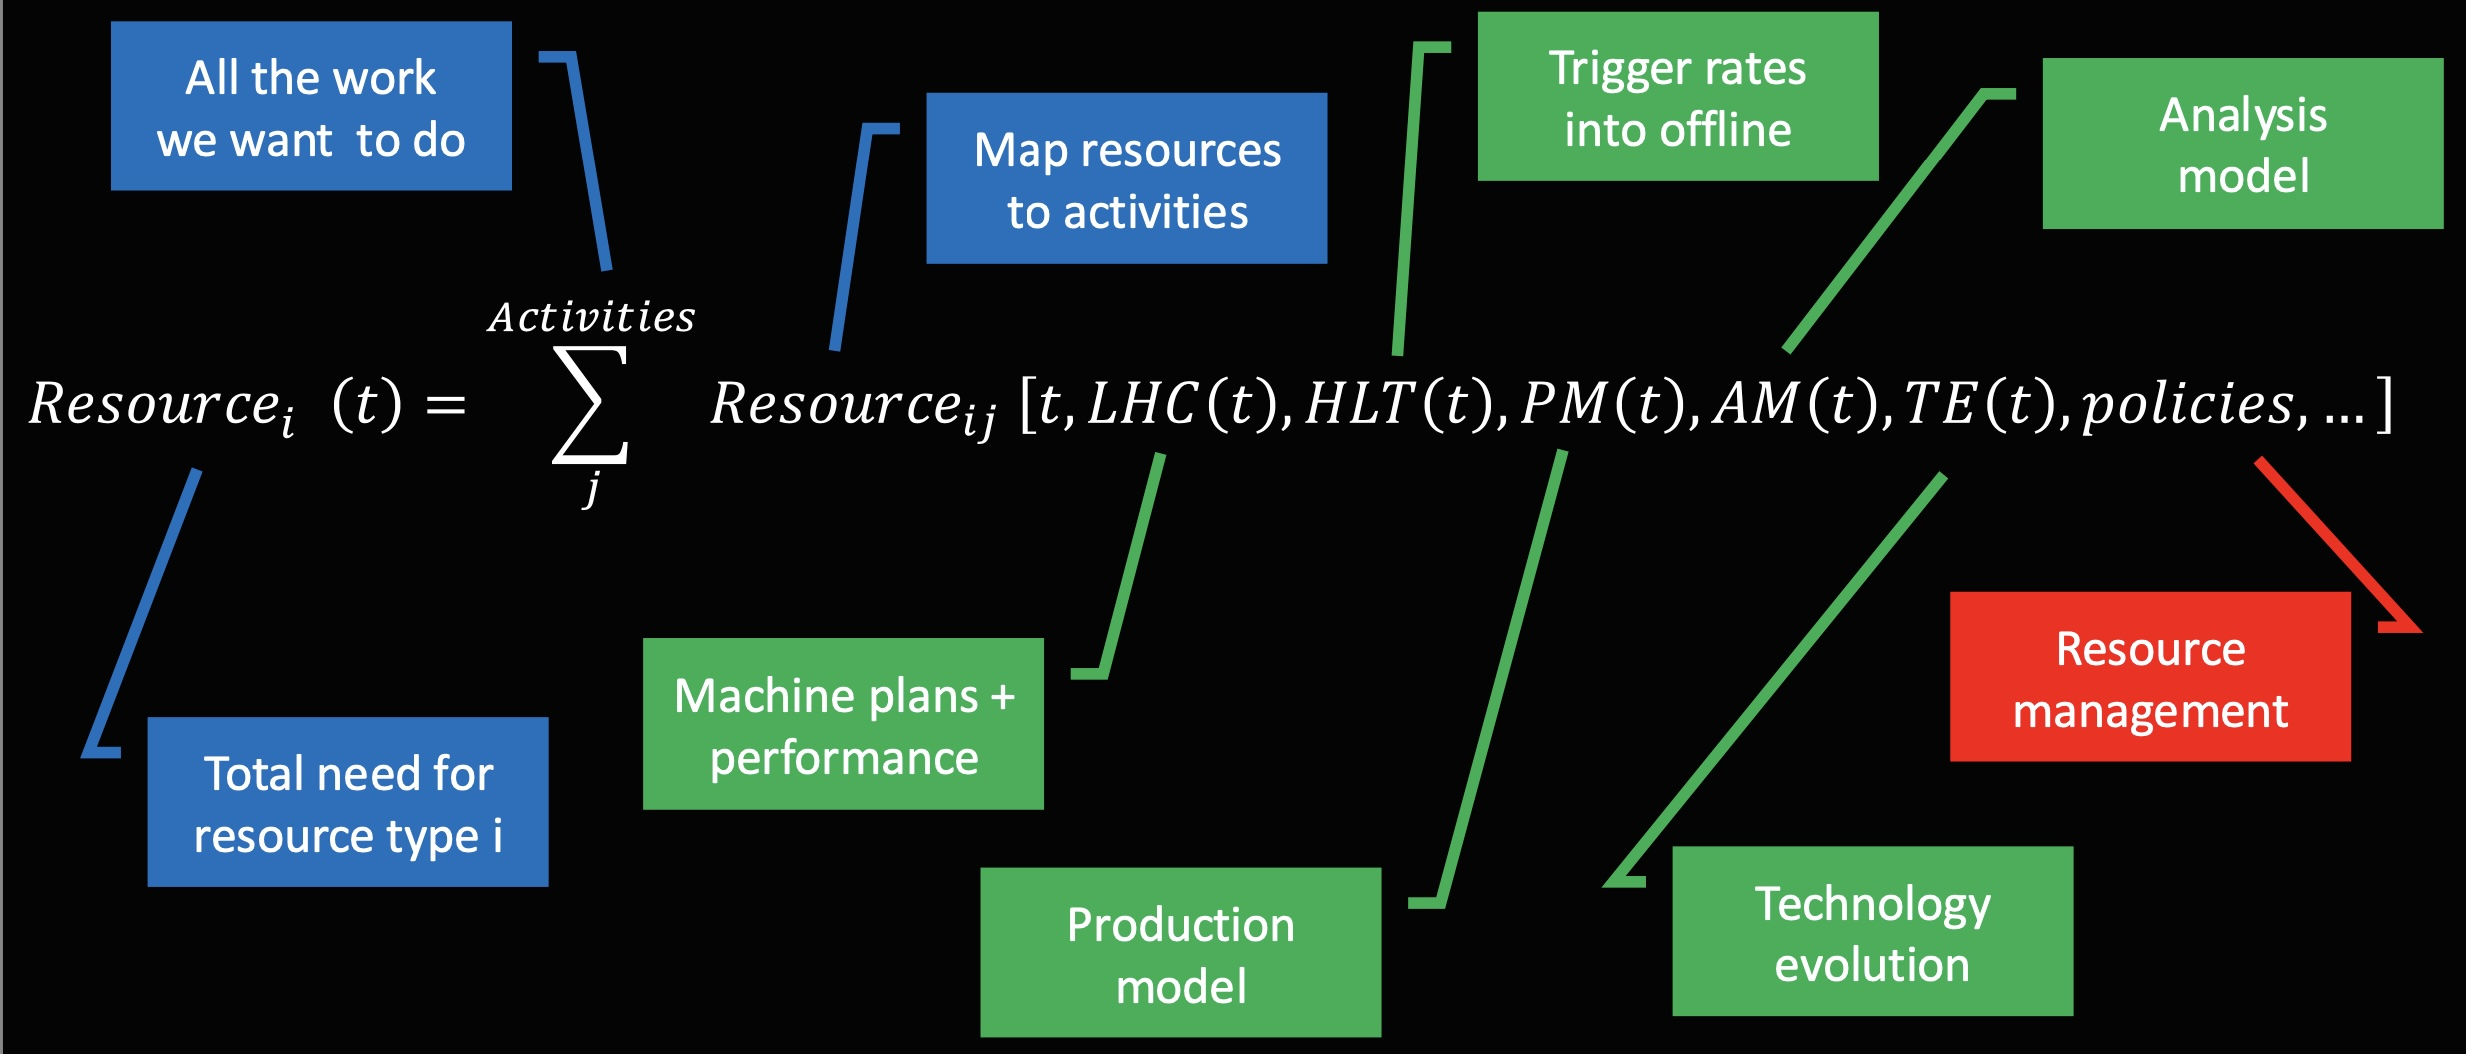
\includegraphics[width=0.7\textwidth]{figs/14 Computing Resource Requirements/CompResFormula.jpg}}
    \caption{Mathematical formulation of the CMS computing resource estimation model.}
    \label{fig:resourceformula}
\end{figure}

The \gls{CPU} is assessed as the total HS23-seconds required for all activities during the year, and thus corresponds to an average resource need. Storage is assessed as the peak need during the year. For modeling, each resource type is broken down into requirements for the different tier levels: \TierZero, \TierOne, and \TierTwo. The \gls{CPU} and disk resources in \TierOne and \TierTwo centers are, however, relatively interchangeable given the large amount of simulation events produced on each. The \gls{HL-LHC} projections presented here are sums across all tier levels. 

Annual projections are made by assessing each activity required by CMS during the year. The set of activities considered in the model has remained relatively static, even as year-to-year variations have occurred. For detector data processing, activities consist of the prompt reconstruction, an end-of-year reprocessing of the \gls{RAW} data (including any data not processed during the prompt reconstruction), a recreation of MiniAOD samples beginning from the \gls{AOD} format, and several updates of the NanoAOD samples starting from MiniAOD. The prompt reconstruction, as well as the end-of-year reprocessing, includes repacking the \gls{RAW} data, producing \gls{AOD}, MiniAOD, NanoAOD, and skims, performing data quality monitoring, and producing alignment and calibration samples. For prompt reconstruction, the assumption is that there is a 48-hour delay for creating calibration data and the capacity to keep up with peak LHC running on a weekly basis. For example, the prompt reconstruction facility requires auxiliary capacity to avoid falling behind during weeks when the LHC is performing better than average.

For simulated samples, activities include physics generation, detector simulation, signal modeling, trigger emulation, creation of simulated \gls{RAW} data, and production of AODSim, MiniAODSim, and NanoAODSim data samples. Two small \gls{MC} simulation production campaigns are included to deliver calibration constants and corrections before data taking, as well as to support the detector commissioning effort at startup. A larger simulation campaign for analysis is considered to begin during its corresponding data-taking period and to continue through the following year. 

Requirements for needs other than detector or simulated data processing are added as a separate component in the resource projections. These include running computing services at CERN, user disk storage at \TierTwo sites, and CERN and operational staging space. Analysis activities on central resources are also included in the resource needs modeling, a decision that deviates from past and current (\PhaseOne) practices.

The total \gls{CPU}, disk, and tape needed is computed as the sum of the needs for each activity. Additional storage, consistent with the replication factor, for data on disk and tape is also accounted for. Activity needs are tabulated as \gls{CPU} or storage required as a function of pileup. Derived \gls{RECO} formats, tiers other than \gls{RAW}, are retained for as long as they are the current best version. Smaller tiers are replicated multiple times, e.g., at most twice for MiniAOD, and three times for NanoAOD in the \gls{HL-LHC} era. Larger tiers are either kept only on tape or removed from disk as they age under the assumption that the newest data is of highest interest to the collaboration. Data and simulated samples that are no longer the current best version are removed from both disk (after 6--24 months) and tape (after 12--36 months), giving some time for analysis activities to either complete or transition. These periods are considerably shorter than historical CMS practice.

The modeling of resource needs also includes analysis activities using central resources. While the \PhaseTwo analysis model includes both batch-oriented and interactive analysis activities (e.g., on analysis facilities), estimates are made from historical CRAB usage and scaled up by the size of the relevant analysis data set. While there is not yet a solid estimate of needs related to the use of dedicated analysis facilities, this assumption is based on the idea that analysis facilities available to all collaborators fit within a similar resource envelope to the current purely batch-based analysis system (scaled up by the number of physics events to be analyzed) and would considerably reduce the need for batch/Grid analysis work.


\subsection{Resource projections}
\label{resourceprojections}

Resource projections are calculated annually for each resource category. Projected \gls{CPU}, disk and tape needs are summarized in Figs.~\ref{fig:cpu_total_projection},~\ref{fig:disk_total_projection}, and~\ref{fig:tape_total_projection}, respectively.
The baseline (or nominal) scenario corresponds to the current performance of the \gls{HL-LHC} software and the planned storage policies. R\&D scenarios are further explored by changing the model parameters and the set of activities before rerunning the simulation. Two additional bands are included that represent the expected growth of resource capacity. 
The lower band corresponds to the resource growth expected by the WLCG Collaboration based on a recent analysis of the evolution of computing and storage costs: $(10 \pm 5)\%$ for \gls{CPU} and tape, and $(5 \pm 5)\%$ for disk storage. The higher band corresponds to the assumptions used for projections made in 2021 and used in previous CMS computing resource estimate results. These projected that sites would be able to increase their total compute and storage capacity by $(15 \pm 5)\%$ per year across all resource types. 
The starting point for projecting these bands is the CMS computing resource request for 2025.  To put this in perspective, the actual resource growth, measured by annual CMS resource requests, has averaged about 15\% for CPU, 18\% for disk, and 23\% for tape since the start of Run 2.

Figure~\ref{fig:cpu_total_projection} shows a gap between \gls{CPU} needs and availability for the baseline scenario throughout \PhaseTwo (solid line). 
Although a successful outcome for the high-probability (H) R\&D scenario (round markers) would reduce \gls{CPU} resource needs, it would not be sufficient to achieve a level within the range of available resources (gray band). Furthermore, failure of the medium-probability (H+M and H+M$^{\prime}$) scenarios (triangular markers) would require either additional resources beyond expectations or changes to the computing model, likely impacting the CMS physics program.
The medium and low (H+M+L) probability scenarios offer reassurance that the gap between \gls{CPU} needs and availability can be bridged. While the H scenario mostly relies on code and algorithm optimization, the medium scenarios rely on fast simulation options, ML applications, and the offloading of a significant amount of code to \gls{GPU}. 
The latter requires sustained, skilled effort to achieve and should be funded with high priority to avoid the need to increase the computing resource budget during HL-LHC.

Figure~\ref{fig:disk_total_projection} illustrates the needs-to-availability gap in disk resources. Recent pricing trends indicate that a 5\% improvement in spending power is a good choice for disk resources.  All R\&D scenarios lie outside the range of predicted available resources (gray band) starting after the first year of the run.  Recent pricing trends are considerably lower than historical trends and will have a large impact on storage capacity for HL-LHC if they continue for the foreseeable future. In this case, CMS will need to consider either reducing the event rate, which is already lower than extrapolated from current \RunThree practice, or restricting analysis even more to very small data tiers.

Tape resource needs are illustrated in Fig.~~\ref{fig:tape_total_projection} and project potential shortages even if the medium and low-probability R\&D scenarios are successful. This situation is also significantly affected by recent trends in storage evolution. CMS will either require additional funding for tape media and infrastructure, prioritize changes to the RAW data format that substantially reduce its size, or consider more drastic changes. Examples of such computing model changes could include removing RAW data from tape after a few years or not storing AOD(Sim) data on the AOD (Sim) tier. 

As mentioned in Sec.~\ref{sec:scouting}, the size of the \gls{L1T} scouting data is not negligible and could amount to 10\% of the \RunFour \gls{RAW} data. Storage for \gls{L1T} scouting data is not accounted for in the resource needs projections, with the implication being that it could be accommodated within the current model if the performance-to-price ratio evolved more favorably than expected, additional funding became available, or at the expense of revising down other storage priorities. A quantitative evaluation will follow an update of the \gls{L1T} scouting strategy within the physics program. 

Figure~\ref{fig:gpu_total_projection} shows the same set of projections for the estimated total \gls{GPU} processing needs. Here, need is expressed in terms of HS23-seconds offloaded, because the \gls{GPU} needs of yet-to-be-developed algorithms are difficult to estimate, and there is not yet a standard metric for \gls{GPU} processing capability. 
%no longer true
%Note that the low-probability scenario offloads less HS23-seconds to \glspl{GPU} than the medium and high scenarios because it involves a significant reduction in \gls{CPU} time through ultra-fast simulation.
Section~\ref{sec:processing-roadmap} describes current estimates for the conversion of HS23 units into the actual needed \glspl{GPU} based on algorithms already running on NVIDIA \glspl{GPU}.

Figure~\ref{fig:resource_pies} shows the expected breakdown of each resource type by processing activity or data type for the baseline %(no R\&D) 
scenario. 
For \gls{CPU}, this includes data reconstruction (``RECO'''), event generation (``GEN'''), detector simulation (``\gls{SIM}''), digitization (``\gls{DIGI}''), and reconstruction of the simulated data (``RECOSim''), as well as analysis data tier activities. These include centralized processing (``reMINIAOD'') and analysis (``Analysis''). This figure indicates that the most profitable areas for additional R\&D effort are RAW data compression for tape and improvements to the miniAOD data model and operational efficiency for disk. It is imperative that CMS address these storage challenges during \LSThree.

\begin{figure}[bhp]
    \centering
    \fbox{
\includegraphics[width=0.8\textwidth]{figs/computing_model/resource_projections/Total_CPU.pdf}}
    \caption{Estimated total \gls{CPU} needs annually through the middle of \gls{HL-LHC} \RunFive. Blue curves correspond to annual projections of needs for the baseline scenario and separately for each of the R\&D scenarios. Two bands (grey, horizontal hatching, and orange-brown, vertical hatching) 
    correspond to the current and previous WLCG guidance for anticipated resource growth.}
    \label{fig:cpu_total_projection}
\end{figure}

\begin{figure}[bhp]
    \centering
    \fbox{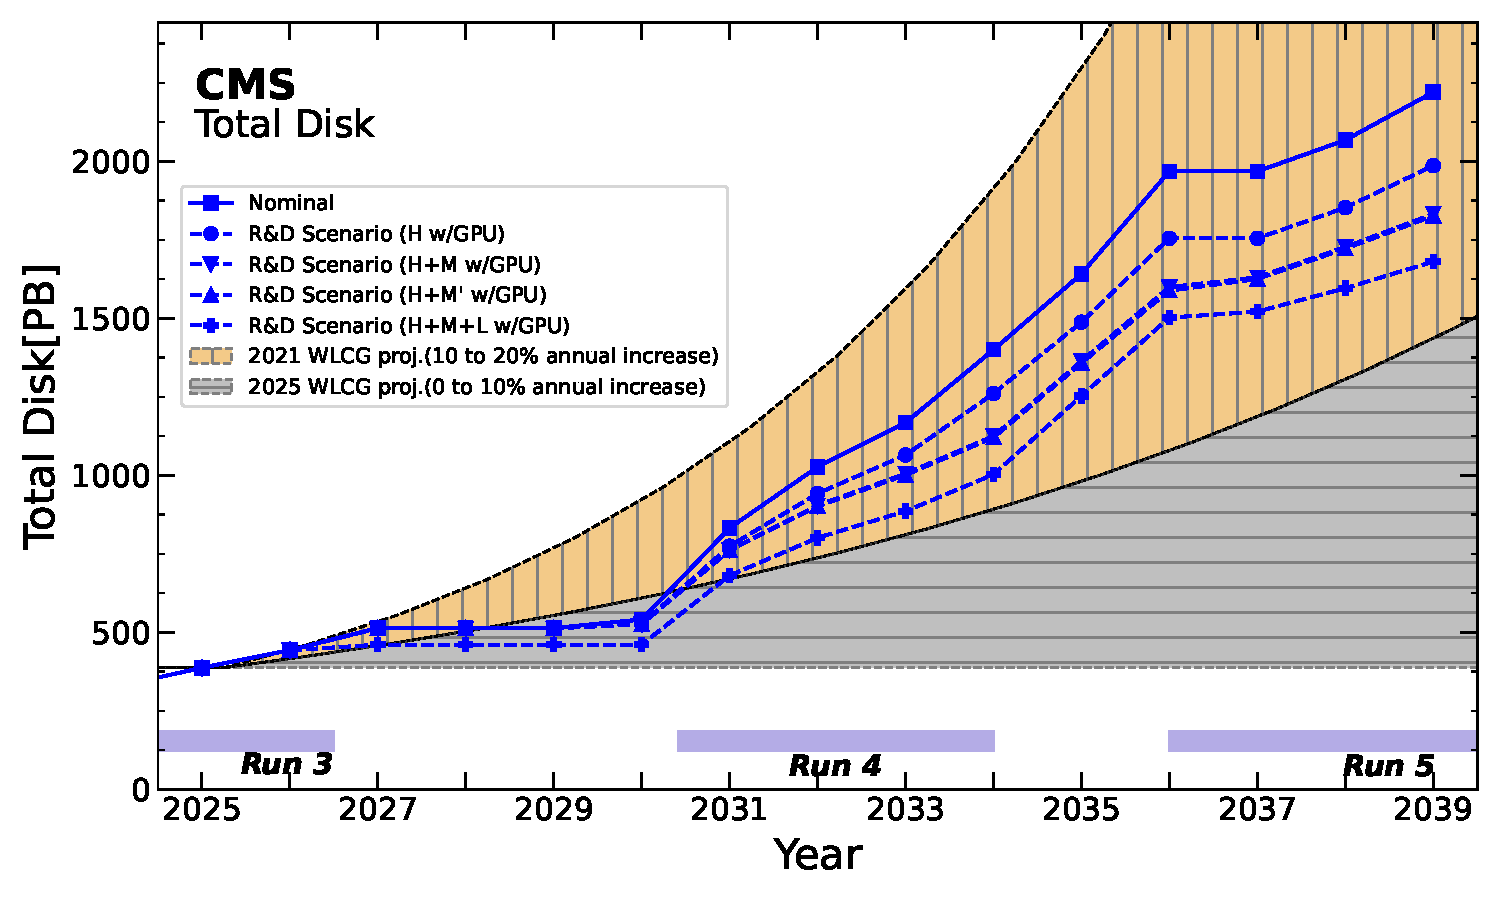
\includegraphics[width=0.8\textwidth]{figs/computing_model/resource_projections/Total_Disk.pdf}}
    \caption{Estimated total disk storage needs annually through the middle of \gls{HL-LHC} \RunFive. Blue curves correspond to annual projections of needs for the baseline scenario and separately each of the R\&D scenarios. Two bands (grey, with horizontal hatching, and orange-brown, with vertical hatching) correspond to the current and previous WLCG guidance on anticipated resource growth.}
    \label{fig:disk_total_projection}
\end{figure}

\begin{figure}[bhp]
    \centering
    \fbox{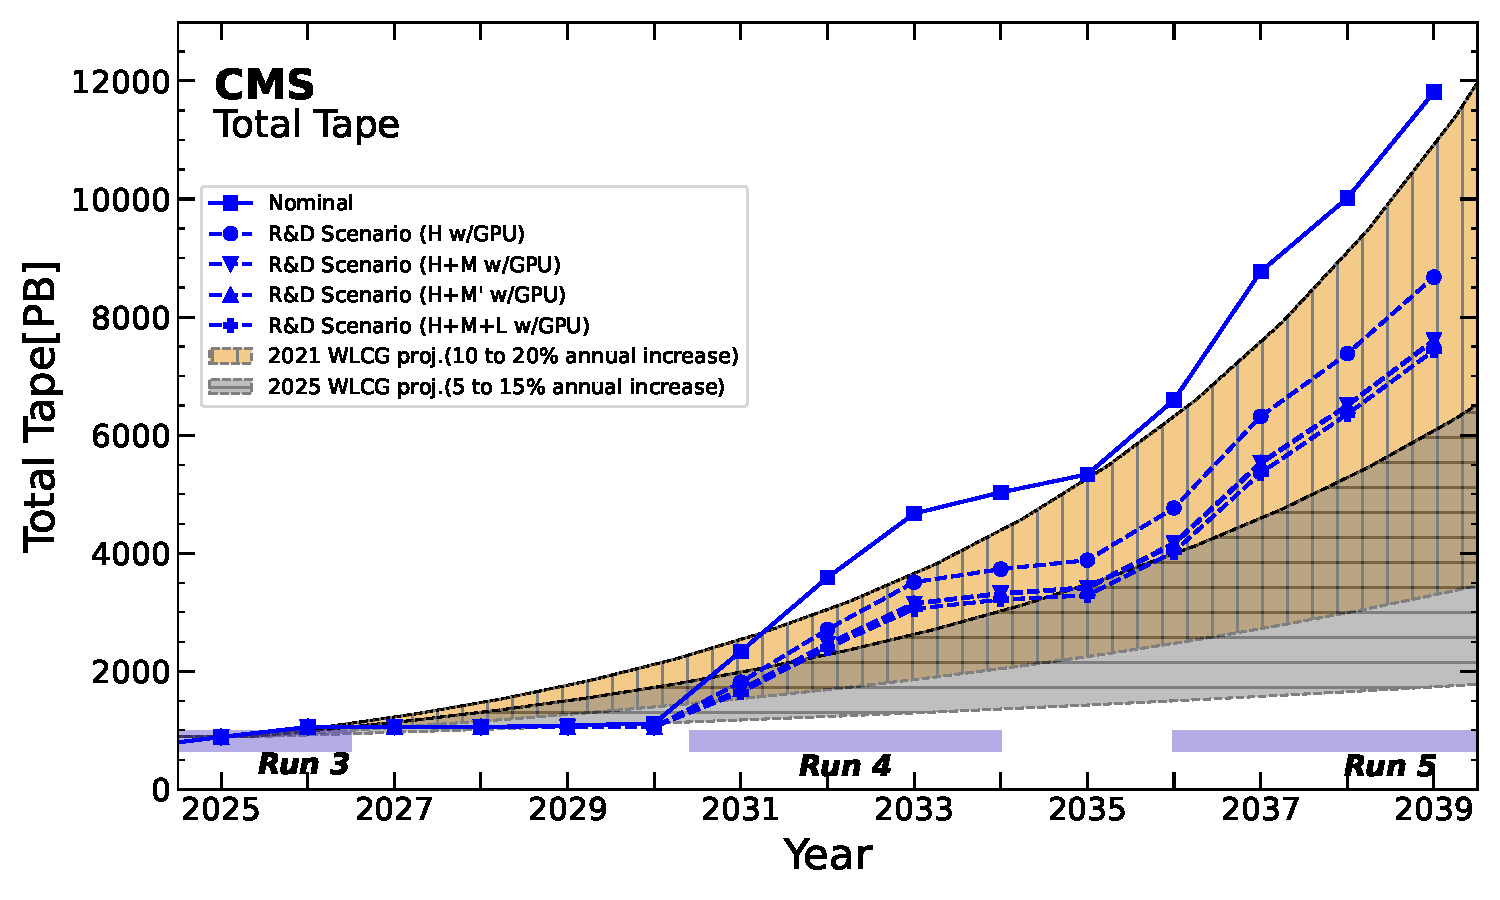
\includegraphics[width=0.8\textwidth]{figs/computing_model/resource_projections/Total_Tape.pdf}}
    \caption{Estimated total tape storage needs annually through the middle of \gls{HL-LHC} \RunFive. Blue curves correspond to annual projections of needs for the baseline scenario and separately for each of the R\&D scenarios. Two bands (grey, with horizontal hatching, and orange-brown, with vertical hatching) correspond to the current and previous WLCG guidance on anticipated resource growth.}
    \label{fig:tape_total_projection}
\end{figure}

\begin{figure}[bhp]
    \centering
    \fbox{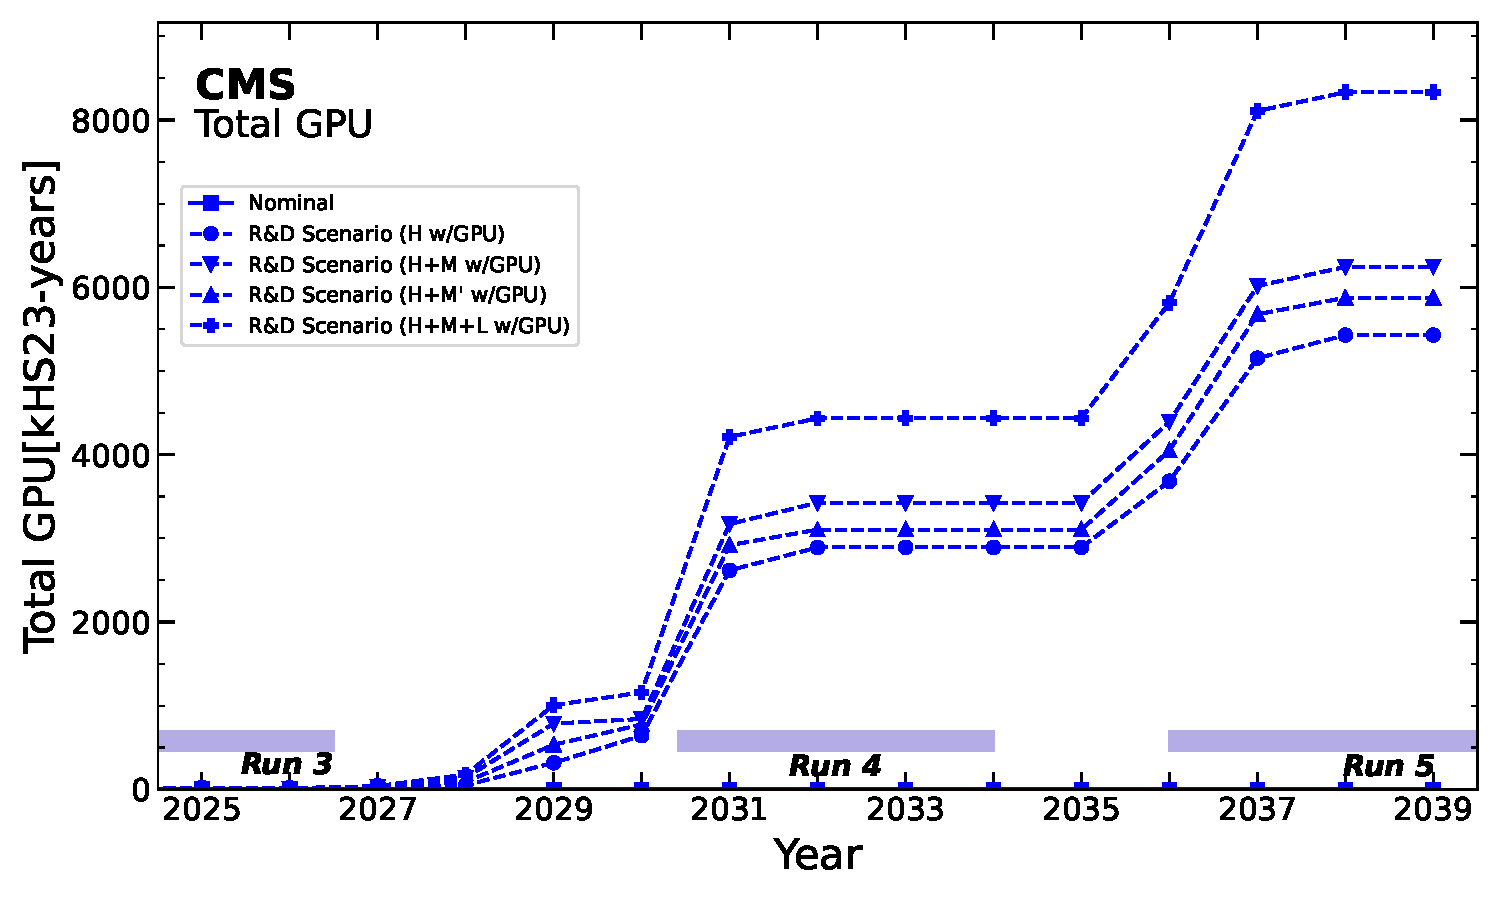
\includegraphics[width=0.8\textwidth]{figs/computing_model/resource_projections/Total_GPU.pdf}}
    \caption{Estimated total \gls{GPU} processing needs annually through \gls{HL-LHC} \RunFive. Need is expressed in terms of HS23 that has been offloaded. Blue curves correspond to annual projections of needs for the baseline scenario and separately for each of the R\&D scenarios. Section~\ref{sec:processing-roadmap} describes current estimates for the conversion of HS23 units into the actual needed \glspl{GPU}.}
    \label{fig:gpu_total_projection}
\end{figure}

\begin{figure}[bhp]
    \centering
    \fbox{
\includegraphics[width=0.42\textwidth]{figs/computing_model/resource_projections/CPU_Pie.pdf}}
    \fbox{
\includegraphics[width=0.42\textwidth]{figs/computing_model/resource_projections/Disk_Pie.pdf}}
    \fbox{
\includegraphics[width=0.42\textwidth]{figs/computing_model/resource_projections/Tape_Pie.pdf}}
    \caption{Breakdown of \gls{CPU}, disk, and tape needs by activity during 2032 (representative year during \RunFour) for the baseline scenario}
    \label{fig:resource_pies}
\end{figure}


\subsection{Sensitivity analysis on the baseline scenario}

\begin{table}[tbph]
	\centering
    \caption{Effects of the variations listed in Table~\ref{tab:CMS-inputs} on the default scenario for 2033 as a baseline.}
    \begin{tabular}{|l|r|r|r|}
    \hline 
    \rowcolor{tableheader}                Parameter                &  \multicolumn{3}{c|}{Impact in 2033} \\
    \rowcolor{tableheader}                                         &  \gls{CPU} (\%)  &  Disk (\%) &  Tape (\%) \\ \hline \hline
    \cellcolor{tablerowheader} Pileup 200 in \RunFour              &  +35             &  +15       &  +19  \\ \hline
    \cellcolor{tablerowheader} HLT Rate 15\unit{kHz}  (+50\%)      &  +26             &  +16       &  +28  \\ \hline
    \cellcolor{tablerowheader} HLT Rate 5\unit{kHz}   (-50\%)      &  -26             &  -15       &  -28  \\ \hline  
    \cellcolor{tablerowheader} HLT scouting rate (+50\%)           &   +1             &   +4       &   +2  \\ \hline
    \cellcolor{tablerowheader} HLT scouting rate (-50\%)           &   -1             &   -4       &   +2  \\ \hline
    \cellcolor{tablerowheader} Negative weights penalty 2.0 (+0.6) &  +11             &   +6       &   +3  \\ \hline
    \cellcolor{tablerowheader} No negative weights penalty (-0.4)  &  -11             &   -6       &   -3  \\ \hline 
    \cellcolor{tablerowheader} \textsc{Fast}/\textsc{FlashSim} 75\%                  &  -27             &   -1       &   -1  \\ \hline
    \cellcolor{tablerowheader} Prompt reco 30\%                    &  -19             &    0       &  -11  \\ \hline
    \cellcolor{tablerowheader} PCL Delay 21 days                   &    0             &   +8       &    0  \\ \hline
    \cellcolor{tablerowheader} No Reprocessing pass                &  -11             &   -8       &  -14  \\ \hline
    \cellcolor{tablerowheader} All event processing timings +50\%  &  +47             &    0       &    0  \\ \hline
    \cellcolor{tablerowheader} All event processing timings -50\%  &  -47             &    0       &    0  \\ \hline    
    \cellcolor{tablerowheader} All event sizes +50\%               &    0             &  +29       &  +40  \\ \hline  
    \cellcolor{tablerowheader} All event sizes -50\%               &    0             &  -29       &  -40  \\ \hline
    \cellcolor{tablerowheader} RAW replicas on tape = 1.0          &    0             &    0       &  -12  \\ \hline
    \cellcolor{tablerowheader} RAW replicas on tape = 2.0          &    0             &    0       &  +12  \\ \hline     
	\end{tabular}
    \label{tab:Variations-2030}
\end{table}

In Table~\ref{tab:CMS-inputs}, possible variations to the baseline scenario are considered to study the sensitivity of resource projections to input parameters to the computing model. Some represent risks which would increase the resource requirements, such as running with 180 or 200 pileup interactions in \RunFour, while others, such as running with 150 pileup interactions through the end of the \gls{HL-LHC} program, will save resources at the expense of reducing HL-LHC physics capabilities.
Other variations account for mitigation measures that can be taken or not, depending on technology evolution, updates to the physics program, and efficiencies gained in the CMS computing model through R\&D. Examples include the potential elimination of the end-of-year reprocessing pass or a reduction of the number of fully simulated events, in favor of fast simulation options. The effects of these variations or uncertainties on the resource needs are studied using the end of \RunFour (2033) in Table~\ref{tab:Variations-2030} and a run well into run \RunFive (2039) in Table~\ref{tab:Variations-2035}, where stable operating conditions are expected to have been reached for the experiment. 

Resource needs are sensitive to the proton-proton HLT output rate (``HLT Rate'') and compute (storage) needed to process (store) events. The RAW replication rate has a moderate impact on total storage. The use of fast simulation techniques can have a potentially significant impact on computing requirements, as can a change in LHC operations to either higher or lower pileup. 

\begin{table}[tbph]
    \centering
    \caption{Effects of the variations listed in Table~\ref{tab:CMS-inputs} on the default scenario for 2039 as a baseline. }
    \begin{tabular}{|l|r|r|r|}
    \hline 
    \rowcolor{tableheader}     Parameter                           & \multicolumn{3}{c|}{Impact in 2039}         \\
    \rowcolor{tableheader}                                         & CPU (\%)  & Disk (\%) &  Tape (\%) \\ \hline \hline
    \cellcolor{tablerowheader} Pileup 150 in \RunFive              & -18             &  -6       &   -7 \\ \hline
    \cellcolor{tablerowheader} HLT Rate 22.5\unit{kHz}  (+50\%)    & +30             & +20       &  +33 \\ \hline
    \cellcolor{tablerowheader} HLT Rate 7.5\unit{kHz}   (-50\%)    & -30             & -20       &  -33 \\ \hline  
    \cellcolor{tablerowheader} HLT scouting rate (+50\%)           &  +1             &  +5       &   +2 \\ \hline
    \cellcolor{tablerowheader} HLT scouting rate (-50\%)           &  -1             &  -5       &   +2 \\ \hline
    \cellcolor{tablerowheader} Negative weights penalty 2.0 (+0.6) & +10             &  +7       &   +4 \\ \hline
    \cellcolor{tablerowheader} No negative weights penalty (-0.4)  & -10             &  -7       &   -4 \\ \hline 
    \cellcolor{tablerowheader} \textsc{Fast}/\textsc{FlashSim} 75\%                  & -24             &  -1       &   -1 \\ \hline
    \cellcolor{tablerowheader} Prompt reco 30\%                    & -24             &  -4       &  -12 \\ \hline
    \cellcolor{tablerowheader} PCL Delay 21 days                   &   0             &  +8       &    0 \\ \hline
    \cellcolor{tablerowheader} No Reprocessing pass                & -14             & -11       &   -8 \\ \hline
    \cellcolor{tablerowheader} All event processing timings +50\%  & +47             &   0       &    0 \\ \hline
    \cellcolor{tablerowheader} All event processing timings -50\%  & +47             &   0       &    0 \\ \hline    
    \cellcolor{tablerowheader} All event sizes +50\%               &   0             & +34       &  +46 \\ \hline  
    \cellcolor{tablerowheader} All event sizes -50\%               &   0             & +34       &  -46 \\ \hline
    \cellcolor{tablerowheader} RAW replicas on tape = 1.0          &   0             &   0       &  -15 \\ \hline
    \cellcolor{tablerowheader} RAW replicas on tape = 2.0          &   0             &   0       &  +15 \\ \hline     
	\end{tabular}
    \label{tab:Variations-2035}
\end{table}

\subsection{Potential for GPU usage}

Figure~\ref{fig:gpu_total_projection} shows the potential GPU usage in each of the R\&D scenarios. Given the current lack of an agreed upon GPU benchmark, the potential for GPU usage is characterized in terms of kHS23 just as is done for CPU usage. As described in Section~\ref{sec:hardware_roadmap}, the CMS Run 3 HLT operational experience is that 1 NVIDIA Tesla T4 GPU is equivalent to approximately 700 HS06 given the set of CMSSW algorithms running on GPUs there. 

The processing requirement in Fig.~\ref{fig:gpu_total_projection} corresponds to the estimated maximum GPU usage by CMS for the set of workflows considered. Assuming the corresponding algorithm development is complete, this processing need can be met with either CPU or GPU resources by sites depending on what is most cost or operationally effective. Workflows where GPUs are essential, such as the training of large AI models, are not included in the GPU usage at this point.

\begin{figure}[bhp]
    \centering
    \fbox{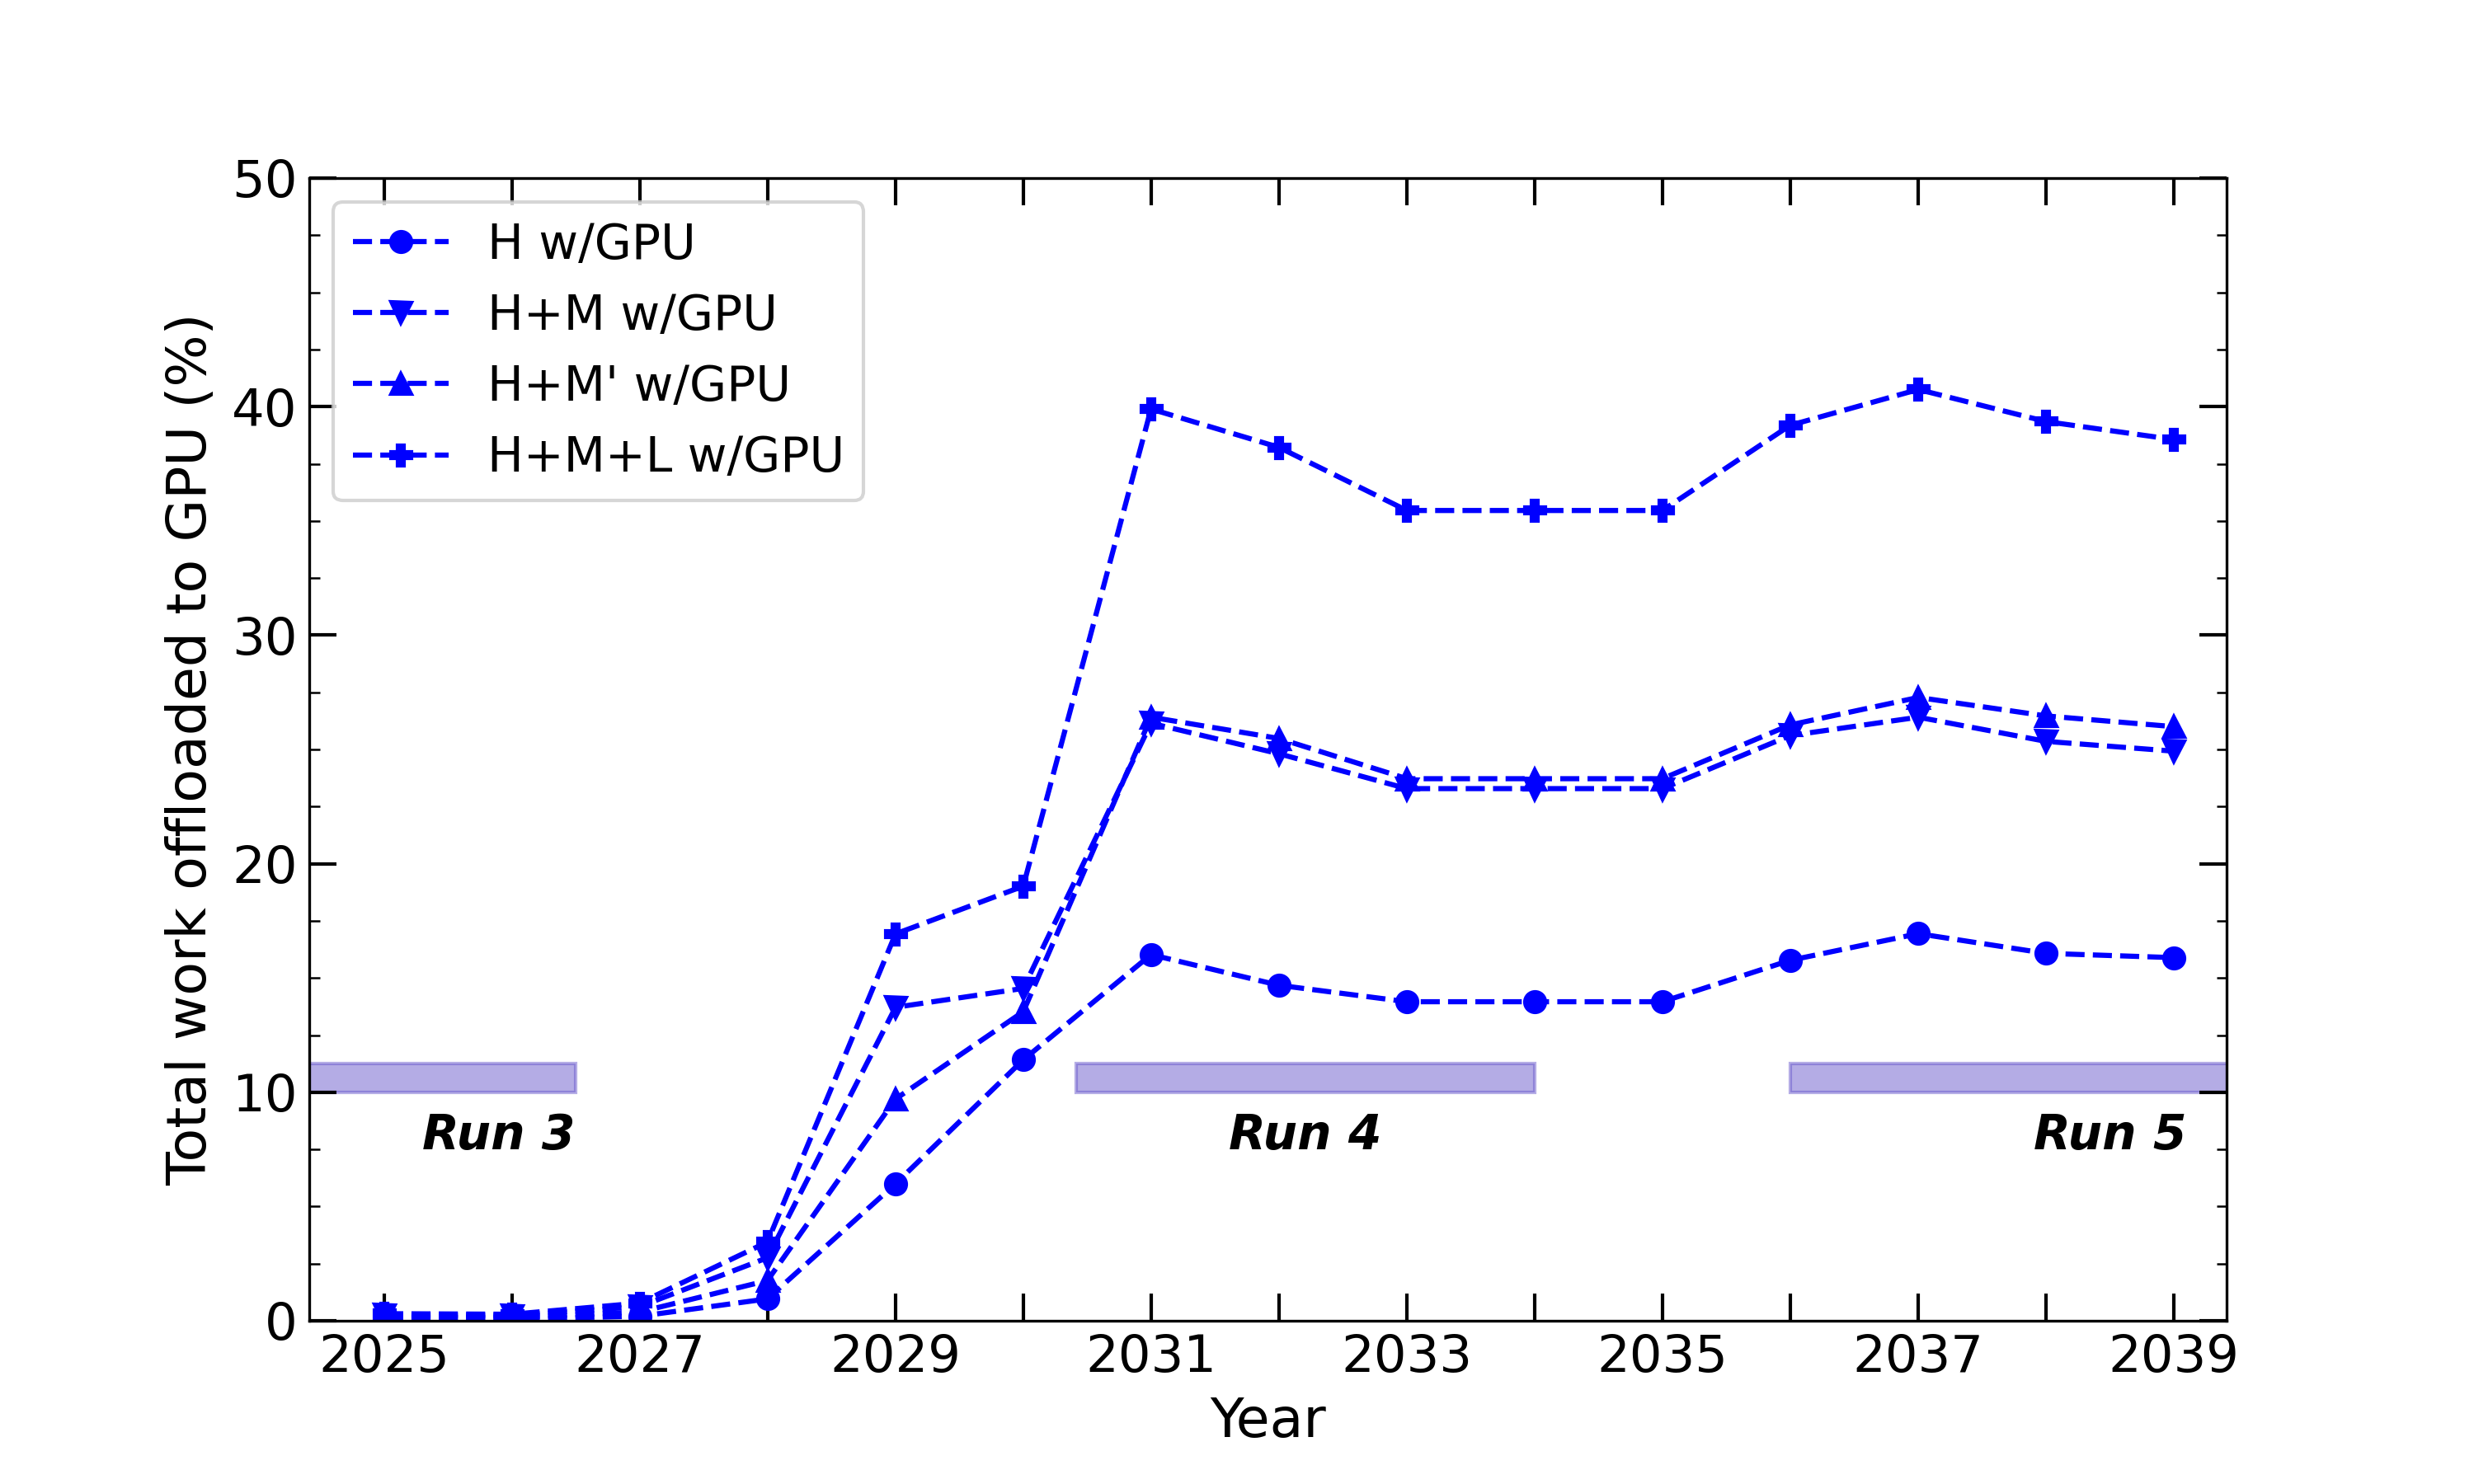
\includegraphics[width=0.8\textwidth]{figs/computing_model/resource_projections/gpu_ratio.png}}
     \caption{Estimated processing that can be offloaded to GPUs. Blue curves correspond to annual projections of needs for each of the R\&D scenarios.}
    \label{fig:gpu-offload-fract}
\end{figure}

Figure~\ref{fig:gpu-offload-fract} shows the estimated GPU offload percentage for each of the R\&D scenarios as a function of time (the baseline scenario has no GPU offload).
The total GPU offload percentage is estimated to be 27\% (48\%) in the prompt reconstruction workflow for the H (H+M+L) scenario during Run 4. For the full \gls{MC} simulation chain, the corresponding percentage is 12\% (35\%). 

\clearpage
%%%%%%%%%%%%%%%%%%%%%%%%%%%%%%%%%%%%%%%%%%%%%%%%%%%%%%%%%%%%%%%%%%%%%%%%%%%%%%%%
%
% technical roadmapMAP
%
%%%%%%%%%%%%%%%%%%%%%%%%%%%%%%%%%%%%%%%%%%%%%%%%%%%%%%%%%%%%%%%%%%%%%%%%%%%%%%%%
% \clearpage
% \input{tex/14_technical_roadmap.tex}
\section{Technical roadmap}
\label{sec:Roadmap}

The CMS \gls{OANDC} technical roadmap is a research and development plan that defines timelines, milestones, effort, risks, dependencies, and deliverables for the tools and products that compose the integrated computing system serving the CMS \PhaseTwo physics program. It must fit the expected funding profile and account for contingency. It is outside the scope of this \gls{CDR}, will be produced as the next step, and would be included in a \gls{TDR} if a decision is made to compose one. A high-level version of the CMS \gls{OANDC} \PhaseTwo technical roadmap is displayed in Table~\ref{tab:CMS-roadmap2}, an evolution of the one included in Ref.~\cite{Software:2815292}. For the main infrastructure and software elements, including internal and external tools, it lists significant milestones and delivery timelines. It also incorporates the planned \gls{CSA} and \gls{DC} exercises, synchronizing the \gls{OANDC} timeline with detector commissioning milestones.

A key component of the planning process and the technical roadmap is the formulation of a comprehensive \gls{GPU} adoption and deployment strategy. This strategy is shortly mentioned in the plan discussed in Table~\ref{tab:CMS-roadmap2}, and it will need to take into account several interrelated tasks listed here: 
\begin{itemize}
\item benchmarking studies to assess \gls{GPU} utilization and for estimating realistic resource requirements for \glspl{GPU},
\item integration of \gls{GPU} benchmarks into the \gls{WLCG} pledging process,
\item development of a framework for handling mixed hardware configurations (\gls{CPU} and \gls{GPU}) across computing sites, 
\item an assessment of exact needs for \gls{GPU} hardware for different workflows, e.g., there may be a focus on reduced precision for optimizing performance of machine learning workflows, but that may not satisfy the needs of tasks such as event generation and reconstruction that require high numerical precision,
\item management of \gls{GPU} resources and task scheduling to ensure optimal utilization of both \glspl{CPU} and \glspl{GPU} across varied workflows, 
\item evaluation of \gls{GPU} needs for core production tasks and also for ancillary activities (e.g., ML training/analysis),
\item a cost-benefit analysis to assess what resources should be pledged and what can be leveraged opportunistically. 
\end{itemize}
Many of these activities will require collaboration with WLCG and external partners in addition to dedicated effort within CMS. Related risks are discussed in Section~\ref{sec:risks}.

\subsection{Computing, software, and analysis challenges}

The CMS \gls{CSA} challenge consists of a series of large-scale data processing and analysis exercises designed to test and validate the readiness of the CMS computing and software systems ahead of major LHC data-taking periods. CMS conducted three challenges ahead of \RunOne in 2006 (CSA06), 2008 (CSA08), 2010 (CSA10)~\cite{2009:csa}. Towards HL-LHC, the \gls{CSA} plan is to test the complete workflows for offline data handling, data transfer between sites, \gls{MC} simulation production, and also physics analysis. The computing model outlined in this \gls{CDR} incorporates many changes from the current incarnation to address the requirements of the collider, the detector, and the physics challenges posed by the \gls{HL-LHC} program. \gls{CSA} must integrate the prototypes for all components and test them individually and as part of the overall system. 

Synchronization with the current \gls{HL-LHC} schedule requires \gls{CSA} to take place, tentatively, by mid-2028. This timeline would provide CMS with ample time to complete a full-scale integration test and address any issues identified during the process before the detector’s commissioning in 2029. To meet this schedule, the required software and computing infrastructure must be developed and delivered in advance. A small set of physics analyses will be performed as part of the \gls{CSA} to test the use of Grid tools and prototypes of the Analysis Facilities. \gls{CSA} coordination forums need to be established at least one year prior, by mid-2027, to ensure all elements are on track.

\gls{CSA} will test different system components in stages, encompassing a broad range of tasks:
\begin{enumerate}
    \item \textbf{Physics preparation.} Select a set of physics analyses that cover a broad range of use cases. Examples include studies with early data, use of NanoAOD to test Analysis Facilities, use of \gls{AOD} or MiniAOD to test Grid tools, and studies requiring special outputs, e.g., skimmed data.
    \item \textbf{Simulation sample preparation.} data sets modeling the simulation chain up to the \gls{HLT} level, which will be fed to the \TierZero as streamer files, as well as physics signal samples.
    \item \textbf{\TierZero.} All \TierZero functions will be exercised, including
    \begin{enumerate}
        \item \textit{Express Reconstruction:} The output will be utilized for subdetector commissioning and to test data quality monitoring tools, calibration and alignment procedures, and the Prompt Calibration Loop.
        \item \textit{Repacking Workflow:} Repacking of streamer files into physics data sets based on \gls{HLT} information.
        \item \textit{Commissioning and online \gls{DQM}}
        \item \textit{Alignment and Calibration workflows, and \gls{PCL}:} To test the procedure to deliver the offline alignment and calibration constants from the express stream.
        \item \textit{Offline Condition Databases:} The offline Condition Database and Frontier will be stress tested, in the context of an updated or new system.
        \item \textit{Prompt Reconstruction at \TierZero and \TierOne.} The workflow elements to study comprise skim production, analysis data set production (\gls{AOD}, MiniAOD, and NanoAOD formats), distribution of analysis data sets to relevant tiers, and Analysis Facilities, when applicable.
     
    \end{enumerate}
    \item \textbf{Workflow and data set Management.} Tasks will include the evaluation of workflow management procedures and submission infrastructure, data set bookkeeping procedures, disk and tape management operations. Workflows include:
    \begin{enumerate}
        \item \textit{\gls{MC} simulation production} using \gls{WLCG} resources and \gls{HPC} centers.
        \item \textit{Re-reconstruction workflows.}
        \item \textit{Analysis workflows.} Targeting early \gls{HL-LHC} data analysis, \gls{WLCG} and \gls{Grid} tools, as well as Analysis Facilities, will be tested.
    \end{enumerate}
\end{enumerate}

In addition, \gls{CSA} may incorporate physics validation workflows and extended physics analysis exercises, such as offline calibration of physics objects and the derivation of data-\gls{MC} scale factors.

\subsection{Data challenges}

The \gls{DC} is the series of commissioning activities that will assess the readiness of the computing infrastructure in preparation for \gls{HL-LHC}. Data challenges are not experiment-specific, as networks are common across all experiments in \gls{HEP}. Six experiments (ATLAS, CMS, LHCb, ALICE, Belle~II, and DUNE) participated in the 2024 DC.
The main activities of future DCs will include data transfers between the \TierZero and the \TierOne centers (e.g., \gls{RAW} data export and data processing), between \TierOne and \TierTwo centers (e.g., \gls{MC} simulation output). \gls{DC} also aims to test token-based authorization technologies and advanced network monitoring tools.

\subsection{Roadmap management}

The CMS \gls{OANDC} management, including the Upgrade Office (see Chapter~\ref{sec:Management}), will be responsible for generating, reviewing, and updating the technical roadmap, as well as for monitoring progress. The management team will also coordinate the prioritization process, decision-making at forking points, and transitions from research to development and production. This work will be done in close collaboration with the \gls{OANDC} L2 areas and the collaboration Board sub-group for \PhaseTwo Effort in \gls{OANDC}. The team will communicate across CMS area boundaries, including but not limited to \glspl{POG}, \glspl{DPG}, \gls{PPD}, and the trigger (\gls{L1T} and \gls{HLT}) teams. Of paramount importance is to continue and enhance mechanisms for consultation and feedback, as well as co-development with external collaborations (e.g., \gls{WLCG}, Rucio, physics generators, \GEANTfour, \textsc{ROOT}). The Office will also ensure that developments are on track and on schedule, and that all stakeholders are aware of progress so they can plan accordingly. 

\subsection{The road to \RunFour}
Since CSA28 will test the whole computing infrastructure chain, from offline data handling to physics analysis, all CMS coordination areas must be involved in defining its milestones. Table~\ref{tab:CMS-roadmap2} represents an initial attempt at a high-level roadmap for the 2026--2030 period. Scheduling \gls{CSA} in 2028 will provide CMS sufficient time to complete the exercises, analyze results, identify issues, and repeat the process, if necessary, before detector commissioning starts in 2029.

CSA28 will be a three- to six-month-long exercise. It will conclude with a jamboree to review the results from each task, identify issues, and develop potential solutions. If necessary, a follow-up challenge (CSA29) would be scheduled to validate the solutions emerging from the CSA28 process.

\subsubsection{Software}
The timeline for delivering a first version of the final detector geometry, as well as data packing and unpacking software, will be coordinated with the detector groups. Completion of this work by the second half of 2026 would give physics object groups about 1.5 years to study reconstruction performance using \gls{RAW} simulated samples, and deliver the CSA28 on time. It is worth mentioning that packer/unpacker development is an iterative process, and that the final \gls{RAW} data format is not expected before 2029, when the electronics are in place. A \gls{CMSSW} version with the capability to generate simulated events for the development of the trigger menu and for the optimization and calibration of the particle-flow algorithm should be available by the end of 2029. The \gls{CMSSW} production-level release for data taking will be ready in early 2030.

\subsubsection{Computing}
Building the systems associated with the proposed \PhaseTwo computing model is not only a technically challenging enterprise, but stretches CMS resources thin in the context of \RunThree support needs through mid-2026. The proposed roadmap allocates time between the end of \RunThree and the start of CSA28 to upgrade the workflow management system. 
During CSA28, CMS will test the entire offline computing infrastructure, starting with streamer files sent from Point-5. The workflow will include repacking and express reconstruction. The \gls{RAW} output from repacking will be held for prompt reconstruction, with a portion sent to tape for delayed reconstruction. The output files from express reconstruction will feed into the \gls{DQM}, commissioning, alignment, and calibration workflows, including \gls{PCL}. The derived conditions data will be stored in the offline conditions database. Once all conditions data is produced, an automatic trigger will initiate prompt reconstruction and publish data sets in \TierOne centers. The scope of the test may be extended to include, for example, the event display software, online and offline \gls{DQM} tools, the data certification procedure, and conditions data validation. 
Another element to test is the \gls{MC} simulation production workflow, including the tools used to collect requests and push them to central production. Once data sets are available, their distribution to \TierOne and \TierTwo centers will be tested, as well as the use of the novel analysis facilities concept. Once data sets are published, selected analyses should be performed (mainly on NanoAOD data) using both analysis facilities and Grid tools.

%\begin{table}[tbph]
%   \centering
%    \begin{tabular}{|c|c|l|l|}
%    \hline
%    
%    \rowcolor{tableheader} Year &  H  &  \multicolumn{1}{c|}{Software}     &   \multicolumn{1}{c|}{Computing Infrastructure}  \\ \hline
%     \multirow{10}{*}{2025} & \multirow{3}{*}{H2} & Integrate RNTuple Source & \multirow{1}{*}{}  \\
%     & & and OutputModule (Prototype) & \\   \cline{3-4}
%     & & \multicolumn{2}{c|}{Converge on the goals for the CSA among Physics, PPD, Trigger, DPG and O\&C} \\ \cline{2-4}
%     & \multirow{6}{*}{H1} & L1T, TSG MC campaign & MC pilot campaign using ARM \\ \cline{3-3}
%     & & GPU workflows in RelVal  & as opportunistic resources \\ 
%     & & (small offload fraction) & \\ \cline{3-3}
%     & & Report on WM review &  \\ \cline{3-4}
%     &  & \multicolumn{2}{c|}{Present this CDR to CMS Collaboration} \\ \cline{3-4}
% \hline
%    \end{tabular}
%    \caption{High-level description of the CMS \gls{OANDC} upgrade roadmap for 2025 expressed in table format, with a resolution of half a year (H1, H2).}
%    \label{tab:CMS-roadmap}
%\end{table}

\begin{table}[tbph]
	\centering
	\caption{High-level description of the CMS \gls{OANDC} upgrade roadmap for the 2026--2030 period expressed in table format.}
	\begin{tabular}{|c|c|l|l|}
	\hline
    
    \rowcolor{tableheader} Year &  H  &  \multicolumn{1}{c|}{Software}     &   \multicolumn{1}{c|}{Computing Infrastructure}  \\ \hline
%    \rowcolor{tableheader}  \multicolumn{4}{c|}{LHC} \\ \hline 
    
     \multirow{2}{*}{2030} & \multirow{2}{*}{H1} & \multicolumn{2}{c|}{Data taking}  \\ \cline{3-4}
     &   & CMSSW startup release & \\ \hline
     
     \multirow{8}{*}{2029} & \multirow{4}{*}{H2} & Start MC for TSG and particle-flow calib. & \TierZero commissioning \\ \cline{3-3}
     & & Freeze CALO geometry, G4  & \\
     & & and \textsc{ROOT} for 2030; CMSSW version for &  \\
     & & TSG samples, particle-flow calibration & \\ \cline{2-4}
     & \multirow{5}{*}{H1} & \multicolumn{2}{c|}{Closure of experimental area, commissioning starts} \\ \cline{3-4}
     & & Converge on event content & Continue testing \TierZero;   \\
     & & (AOD, Mini, Nano) & targeting detector commissioning. \\ \cline{3-3}
     & & New MC samples for POGs and L1T & \\ \cline{3-3}
     & & Converge on RAW data formats & \\ \hline
     
     \multirow{9}{*}{2028} & \multirow{1}{*}{H2} & \multicolumn{2}{c|}{CSA28 Jamboree (Decision on CSA29 if need)} \\ \cline{2-4}
     & \multirow{6}{*}{H1} & & Prompt processing elements \\
     & & & (\TierZero, PCL, DQM) testing; \\ %\cline{4-4}
     & & & MC workflow testing \\ \cline{3-4}
     & & \multicolumn{2}{c|}{CSA28 starts} \\  \cline{3-4}
     & & CMSSW for CSA & \TierZero, SI, DM, WM, Grid-pool for analysis \\ 
     & & New PU mixing method ready & and analysis facilities ready for CSA28; \\
     & & & Phase out all Run 1/2/3 infrastructure \\ \hline

    \multirow{6}{*}{2027} & \multirow{3}{*}{H2} & \PhaseTwo MC preparation for CSA28 & Tests on infrastructure for CSA28 \\
    & & (up to HLT) & \\ \cline{3-3}
    & & \PhaseTwo Reconstruction jamboree & \\ \cline{2-4}
    & \multirow{3}{*}{H1} & \multicolumn{2}{c|}{CSA28 preparation activities} \\ \cline{3-4}
    %&  & Phase-2 MC campaign for L1T, TSG, POG & New infrastructure exercise \\ \cline{3-4} 
    & & GPU workflows in RelVal & Data Challenge 2027; 50\% of the \\  
    & & (larger offload fraction) & foreseen requirements for HL-LHC \\ \hline

    \multirow{11}{*}{2026} & \multirow{4}{*}{H2} & \PhaseTwo \gls{MC} with agreed geometry used & Initiate infrastructure upgrade \\
    & & for CSA28 preparation and validated & \\
    & & (first version of) packer/unpacker. & \\ \cline{3-4}
    & & \RunThree reprocessing (if any) & \\ \cline{2-4}
    & \multirow{7}{*}{H1} & \multicolumn{2}{c|}{\LSThree starts} \\ \cline{3-4}
    & & GPU workflows in \gls{RelVal} & Finalize the plan for infrastructure \\ 
    & & (larger offload fraction) & update including \TierZero, DMWM, \\  \cline{3-3}
    & & Production-ready RNTuple & CRAB, Analysis facilities \\
    & & Source and OutputModule & \\ \cline{3-4}
    & & 2026 L1T and TSG MC Production & Data taking and \RunThree MC production; \\ \cline{3-3}
    & & Release for 2026 data taking & ARM as opportunistic resources \\
    \hline 
    \end{tabular}
    \label{tab:CMS-roadmap2}
\end{table}

\clearpage
%%%%%%%%%%%%%%%%%%%%%%%%%%%%%%%%%%%%%%%%%%%%%%%%%%%%%%%%%%%%%%%%%%%%%%%%%%%%%%%%
%
% SUMMARY
%
%%%%%%%%%%%%%%%%%%%%%%%%%%%%%%%%%%%%%%%%%%%%%%%%%%%%%%%%%%%%%%%%%%%%%%%%%%%%%%%%
% \clearpage
% \input{tex/15_summary.tex}
\section*{Conclusions}
\addcontentsline{toc}{section}{Conclusions}
\label{Conclusions}

A computing model for the CMS \PhaseTwo experiment is described at the conceptual level, including a baseline and several R\&D scenarios evaluated by their probability of success and adoption. Upgrade O\&C is part of the CMS apparatus, a sub-system, commensurable in complexity, hardware cost, and effort to a detector component. Prioritization, progress tracking, and coordination of CMS management’s decision-making process are important responsibilities of the O\&C organization.

During HL-LHC, CMS will face unprecedented challenges in software and computing. The experience of \RunThree indicates that offline resources will be a limiting factor in fully exploiting the HL-LHC physics program. CMS will need to process and store exabytes of data. Price-per-performance and capacity projections indicate that planned improvements to the software and computing systems will fall short of meeting needs under the current computing model and flat funding assumptions.  While uncertainties are large, it is clear that CMS will have to reevaluate what it stores on disk and tape, given the recent change in WLCG projections.  This will require a change in the computing model. With the most aggressive R\&D assumptions of success, CMS will have sufficient computing resources to process HL-LHC data as planned. Research software engineering effort in the short term will need funding support, but will be compensated for in the long term when successful R\&D is put into production.

As recently demonstrated, technology tracking is essential, and changes in expectations can drastically alter the needed focus of our upgrade efforts. Before the storage projection revisions made in the summer of 2025, CMS focused on processing capabilities. With continued push to deploy the new \gls{GPU} algorithms and \gls{AI} techniques developed for HL-LHC, there is a path to success. However, a refocused effort must also prioritize storage  R\&D in two directions. The first is to use compression and summary techniques to reduce the size of the physics or detector object data within the event data tiers. The second is to minimize the number of copies of data in storage by making policy changes relative to the baseline. These modifications introduce risk to CMS physics analysis capability and increase the risk of potential data loss. The aim of the second R\&D thrust, required to fit within the projected resource envelope, is to reduce the impact of these policy changes on the quality and breadth of CMS physics.

The computing model presented in this conceptual design of the CMS \gls{HL-LHC} computing system describes an R\&D path to successfully bridge the gap between available resources and those needed to deliver on CMS’s full physics program, assuming that the required organization, funding, and support across the full CMS Collaboration are put in place.

%%%%%%%%%%%%%%%%%%%%%%%%%%%%%%%%%%%%%%%%%%%%%%%%%%%%%%%%%%%%%%%%%%%%%%%%%%%%%%%%
\clearpage
% \section{Glossary of special terms and acronyms}

\printglossary[type=\acronymtype,title=Glossary of special terms and acronyms,toctitle=Glossary of special terms and acronyms]
% \printglossary[type=\acronymtype]
\label{Glossary}

%%%%%%%%%%%%%%%%%%%%%%%%%%%%%%%%%%%%%%%%%%%%%%%%%%%%%%%%%%%%%%%%%%%%%%%%%%%%%%%%
\clearpage

\addcontentsline{toc}{section}{References}
\label{References}

\bibliography{TDR-24-001}

% \end{document}
